\chapter{Mascaret}

\section{Introduction}

The predictive skills of hydraulic models have greatly increased with advances in free surface flow numerical modelling and computational resources. Real-time flood forecasting relies on the use of sparse in situ observations as well as imperfect hydrology or hydraulic models usually solving the 1-D Shallow Water Equations (SWE). Assessing the predictive capabilities of these hyperbolic partial differential equations remains an important challenge as public safety and water resource management are at stake~\citep{weerts2011}. SWE solve for spatially varying water level and river discharge (referred to as the river state) using physical parameters (e.g.~friction coefficients, bathymetry), initial conditions and boundary conditions described as a hydrograph or water level time series. These input data are subject to epistemic uncertainties due to an imperfect knowledge of the river properties as well as to aleatory uncertainties related to environmental and meteorological intrinsic hazards. Both types of errors translate into uncertainties in the simulated river state, thus preventing the hydraulic model from being effective in forecast mode. In practice, these uncertainties can be reduced when complementary data become available.

%---Intro to data assimilation 
Data assimilation (DA) offers a convenient framework to reduce model uncertainties by combining observations with the model simulation taking into account errors in both sources of information. Prior to DA, the main sources of uncertainties should be identified and included in the control vector; this is achieved with a sensitivity analysis (SA) study that allows to classify uncertainties in the inputs with respect to their impact on the model outputs, for instance in terms of variance using Sobol' indices~\citep{iooss2016,DeLozzo2017}. Several studies in the framework of hydraulics demonstrated the merits of DA~\citep{barthelemy2015,cloke2009,dechant2011,habert2016,moradkhani2005} to provide a more accurate river state.
This is achieved by inferring an optimal set of parameters (e.g.~river and floodplain friction coefficients, upstream and lateral river discharge, bathymetry) and/or by directly correcting the river state.

%---Ensemble-based data assimilation 
Ensemble-based methods such as the Ensemble Kalman Filter (EnKF)~\citep{durand2008,moradkhani2005,ELSheikh2013} and the Particle Filter (PF)~\citep{matgen2010,parrish2012} are popular algorithms; they articulate as a two-step procedure derived from Bayesian inference: (1)~a forecast step to sample the uncertain inputs and propagate the uncertainty through the model, thus providing an ensemble of river states; and (2)~an analysis step to weight each member or particle of the ensemble based on its discrepancies to the available observations and to derive in the case of parameter estimation, a correction on the inputs that is then propagated to the river states by model integration. In the EnKF algorithm, the weights are provided by the stochastic estimation of covariance matrices between errors in model inputs and outputs. In contrast, in the PF algorithm, the weights correspond to likelihoods associated with the probability density function (PDF) of the control vector conditioned upon the observations; PF provides an alternative to EnKF when the model is subject to strong non-linearity and non-Gaussian errors. 

%---Monte Carlo sampling, issue
Both PF and EnKF algorithms usually rely on Monte Carlo (MC) random sampling techniques to carry out the forecast step, i.e.~sample the uncertain input space and obtain the sample of output variables through the integration of the forward model. Provided these input and output samples, they rely on the stochastic estimation of error statistics such as PDF for PF, covariances between spatially distributed model outputs or covariances between model inputs and outputs for EnKF. MC techniques are generic, robust and easily portable on massively parallel supercomputers; yet they remain computationally expensive due to their slow convergence rate scaling as the inverse of the square root of the number of particles~\citep{lixiu2008}. As shown in~\citet{barthelemy2015} and \citet{bozzi2015}, a large number of forward model evaluations should be carried out to converge the stochastic evaluation of error statistics such as PDFs, Sobol' indices and covariance matrices. This is often not compatible with operational constraints or high-dimensional problems. 

%---How to go beyond Monte Carlo random sampling
To overcome the issue of crude MC techniques, there is a need to develop efficient and robust uncertainty quantification (UQ) methods in the context of DA for hydraulics to limit (1)~the number of significant sources of uncertainties and (2)~the computational cost of quantifying uncertainties on the river state, e.g.~moments (mean, covariance) and PDF, while preserving the accuracy of the mapping $\mathcal{M}$ between the uncertain inputs $\mathbf{x}$ and the vector of $M$ river water heights $\mathbf{h}$:
\begin{equation}
\mathbf{x} \in \mathbb{R}^d \quad \rightarrow \quad \mathbf{h} = \mathcal{M}(\mathbf{x})\in\mathbb{R}^M.
\end{equation}
The key idea of non-intrusive UQ methods is to build a cost-effective surrogate to perform UQ and SA steps~\citep{iooss2010,iooss2016,lamboni2011,lemaitreknio2010,saltelli2007,storlie2009} (see~\cref{sec:surrogate}).

The objective is to evaluate the performance of PC and GP surrogates mimicking the behaviour of 1-D open-channel flows for UQ and SA steps that are important in the design of EnKF and PF algorithms. The quantity of interest is the 1-D water level discretized along 50~km of the Garonne River (South-West France). As a preliminary step, the focus is made on steady flows and the flow remains fluvial. The treatment of strong non-linearity and discontinuity induce by fluvial/super-critical transitions is beyond the scope of this study. The main sources of uncertainties are the upstream discharge that is constant in steady state conditions and the friction coefficient that is a piecewise constant function. Under these hypotheses, the present work features scalar inputs and spatially varying outputs due to the heterogeneous bathymetry of the Garonne River. A convergence study is first carried out to determine the size of the training set $N$ that is required to build a valid surrogate using either PC expansion or GP model. GP and PC surrogates are then compared when a computational budget is set, i.e.~for the same number of snapshots (also called simulations in the paper) $N$ used to construct each surrogate. The comparison is carried out with respect to the following metrics on $\mathbf{h}$: PDF that is of interest for Bayesian inference and PF algorithms; spatially varying Sobol' indices (associated with the correlation between each uncertain input and the spatially distributed output) and correlation matrix (associated with the spatial correlation of the output) that are of interest for variational and EnKF algorithms.

The structure of the chapter is as follows. \Cref{sec:hydrau} introduces the 1-D SWE solved using MASCARET and the Garonne River case study. \Cref{sec:UQresults} presents the results of the comparative study between PC and GP with respect to a MC reference. Conclusions and perspectives are given in~\cref{sec:ccl}.

\section{Hydraulic Modelling}\label{sec:hydrau}

The SWE represent the dynamics of open-channel flows, typically in rivers with small bathymetry variations~\citep{horritt2002}. They form a hyperbolic system of partial differential equations that characterize subcritical and supercritical flows subject to hydraulic jumps. Here, we only deal with subcritical flows, in the plain.

%------> Equations
\subsection{1-D shallow water equations (SWE)}

We consider a 1-D hydraulic model commonly used in hydraulic engineering and flood forecasting. The stream channel is described by a hydraulic axis corresponding to the main flow direction, implying that the river channel is represented by a series of cross-sections (or profiles) identified by a curvilinear abscissa $a$ ranging from $a_{\text{in}}$ upstream of the river to $a_{\text{out}}$ downstream. 1-D SWE are derived from mass conservation and momentum conservation. The equations are written in terms of discharge (or flow rate) $Q$~(m$^3$\,s$^{-1}$) and hydraulic section $A$~(m$^2$) that relates to water level (or water height) $h$~(m) such that $A \equiv A(h)$. The non-conservative form of the 1-D SWE for non-stationary flow reads~\citep{thual2010} 
\begin{eqnarray}
\left\{
\begin{array}{l}
\displaystyle{\partial_t A(h) + \partial_a Q=0} \\
\displaystyle{\partial_t Q +  \partial_a\left(\frac{Q(h)^2}{A(h)}\right) + g\,A(h)\,\partial_a h - g\,A(h)\,(S_0-S_f) = 0} \\
\end{array}
\right.
\label{eq:SWE}
\end{eqnarray}
with $g$ the gravity, $S_0$ the channel slope and $S_f$ the friction slope. In the present study, the SWE are combined with the Manning-Strickler formula to parameterize the friction slope $S_f$ such as:
\begin{equation}
S_f = \frac{Q^2}{K_s^2\,A(h)^{2}\,R(h)^{4/3}},   
\label{eq:friction}
\end{equation}
where $R(h) =A(h)/P(h)$~(m) is the hydraulic radius written as a function of the wet perimeter $P(h)$, and where $K_s$~(m$^{1/3}$\,s$^{-1})$ is the Strickler friction coefficient. The pair $(h,Q)$ forms the hydraulic state varying in time and space. For steady flows in case of smooth solutions, \cref{eq:SWE} simplifies to: 
\begin{eqnarray}
\left\{
\begin{array}{l}
\displaystyle{\partial_a Q=0} \\ \\
\displaystyle{\partial_a h =\frac{(S_0-S_f)}{1-Fr^ 2}}\\
\end{array}
\right.
\label{eq:backwater}
\end{eqnarray}
where $Fr$ is the dimensionless Froude number 
\begin{equation}
Fr^2 = \frac{Q^2}{gA^3} \frac{\partial{A}}{\partial{h}}.
\label{eq:froude}
\end{equation}

The solutions for~\cref{eq:backwater} are called {\it backwater curves} when the downstream boundary condition is prescribed in a deterministic way for subcritical flow. To solve~\cref{eq:backwater}, the following input data are required: bathymetry, upstream or downstream boundary conditions, lateral inflows and roughness coefficients. It should be noted that the evolution in time of the bathymetry or the roughness coefficient is not taken into account in this study. The imperfect description of this data translates into errors in the simulated hydraulic state $h$. To understand the structure of these errors, it is of prime importance to determine which input variables contribute, and to what extent, to the variability in the hydraulic state at different curvilinear abscissas $a$ along the river channel, for instance via a SA study (\cref{sec:SA}).

We use the MASCARET software to simulate the 1-D SWE in~\cref{eq:SWE} and predict $(h, Q)$ along the discretized curvilinear abscissa of the hydraulic network $a \in [a_{\text{in}}, a_{\text{out}}]$. The SWE are solved here with the steady kernel of MASCARET based on a finite difference scheme~\citep{goutal2002,goutal2012}, meaning that $(h,Q)$ only varies in space. MASCARET is part of the TELEMAC-MASCARET open-source modelling package developed at EDF (\textit{Électricité de France} R\&D) in collaboration with CEREMA (\textit{Centre d'Étude et d'expertise sur les Risques, l'Environnement, la Mobilité et l'Aménagement}); it is commonly used for dam-break wave simulation, reservoirs flushing and flooding. 

%------> Hydraulic model
\subsection{Garonne River Case Study}

The present study is carried out on a real hydraulic network over the Garonne River in South-West France. The Garonne river flows along 647~km from the Pyrenees to the Atlantic Ocean draining an area of $55,000$~km$^2$ (corresponding to the fourth-largest river in France). The present study focuses on a 50 km reach from Tonneins ($a_{\text{in}} = 13$~km) to La Réole ($a_{\text{out}} = 62$~km) with one observing station at Marmande ($a = 36$~km) as presented in~\cref{fig:garonne}a. The mean slope over the reach is $S_0 = 3.3$~m\,km$^{-1}$; the mean width of the river is $W = 250$~m; the bank-full discharge is approximately $\overline{Q} = 2550$~m$^3$\,s$^{-1}$. Despite the existence of active floodplains, this reach can be accurately modelled by a 1-D hydraulic model using~\cref{eq:SWE}~\citep{besnard2011}.

\Cref{fig:garonne}b presents the non-uniform bathymetry profile along the 50-km reach, interpolated from $83$ on-site bathymetry cross-sections. Friction for the river channel and its floodplain is prescribed over three zones separated by dashed lines. The Strickler coefficients $K_{s_1}$, $K_{s_2}$ and $K_{s_3}$ are used to characterize friction through~\cref{eq:friction} and are uniform per zone. The observing station at Marmande is located at the beginning of the third zone associated with $K_{s_3}$. 

\begin{figure}[!h]
\centering
\subfloat[]{
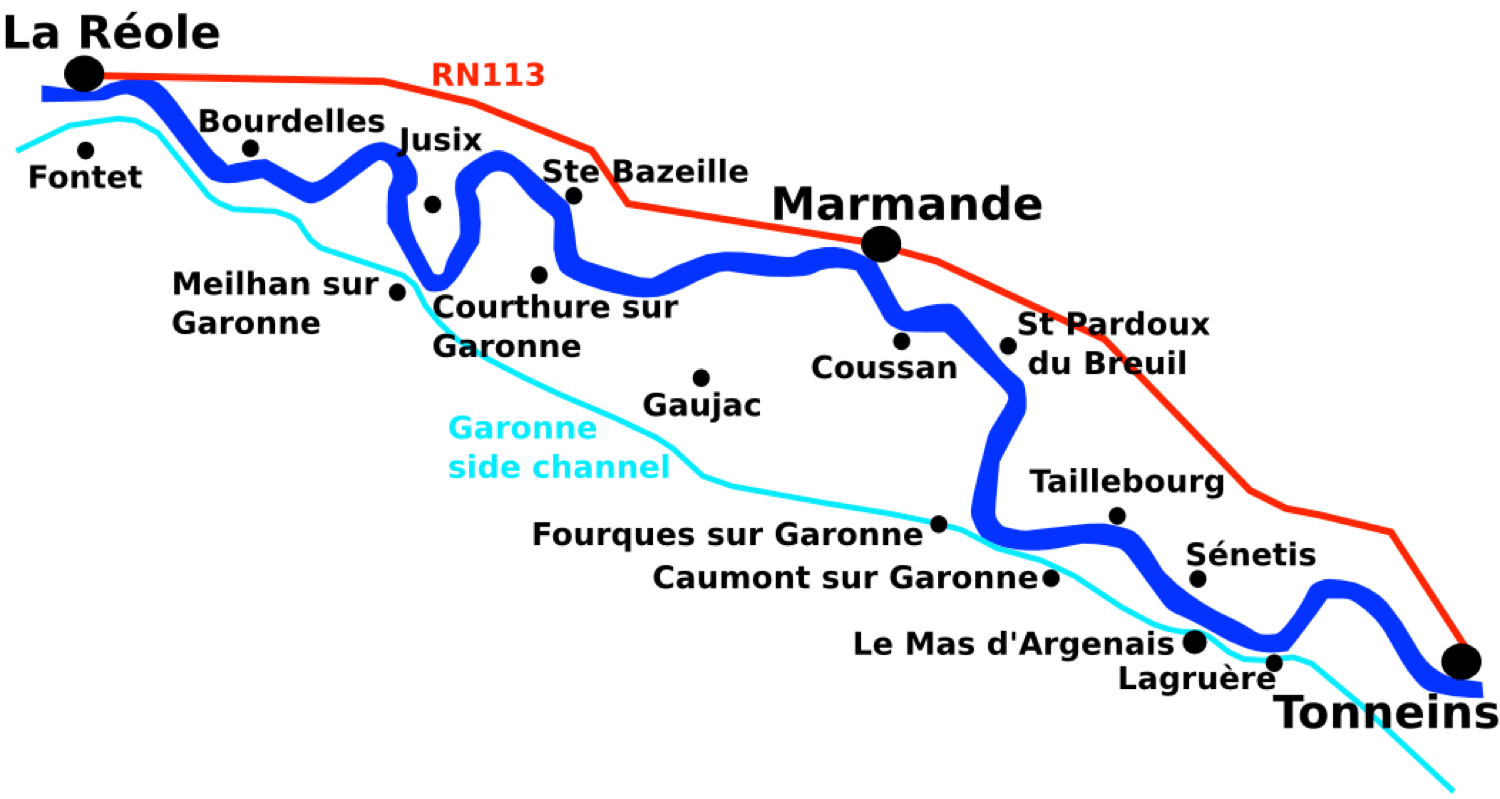
\includegraphics[width=0.9\linewidth,height=\textheight,keepaspectratio]{fig/applications/mascaret/Fig1a.pdf}}
     
\subfloat[]{
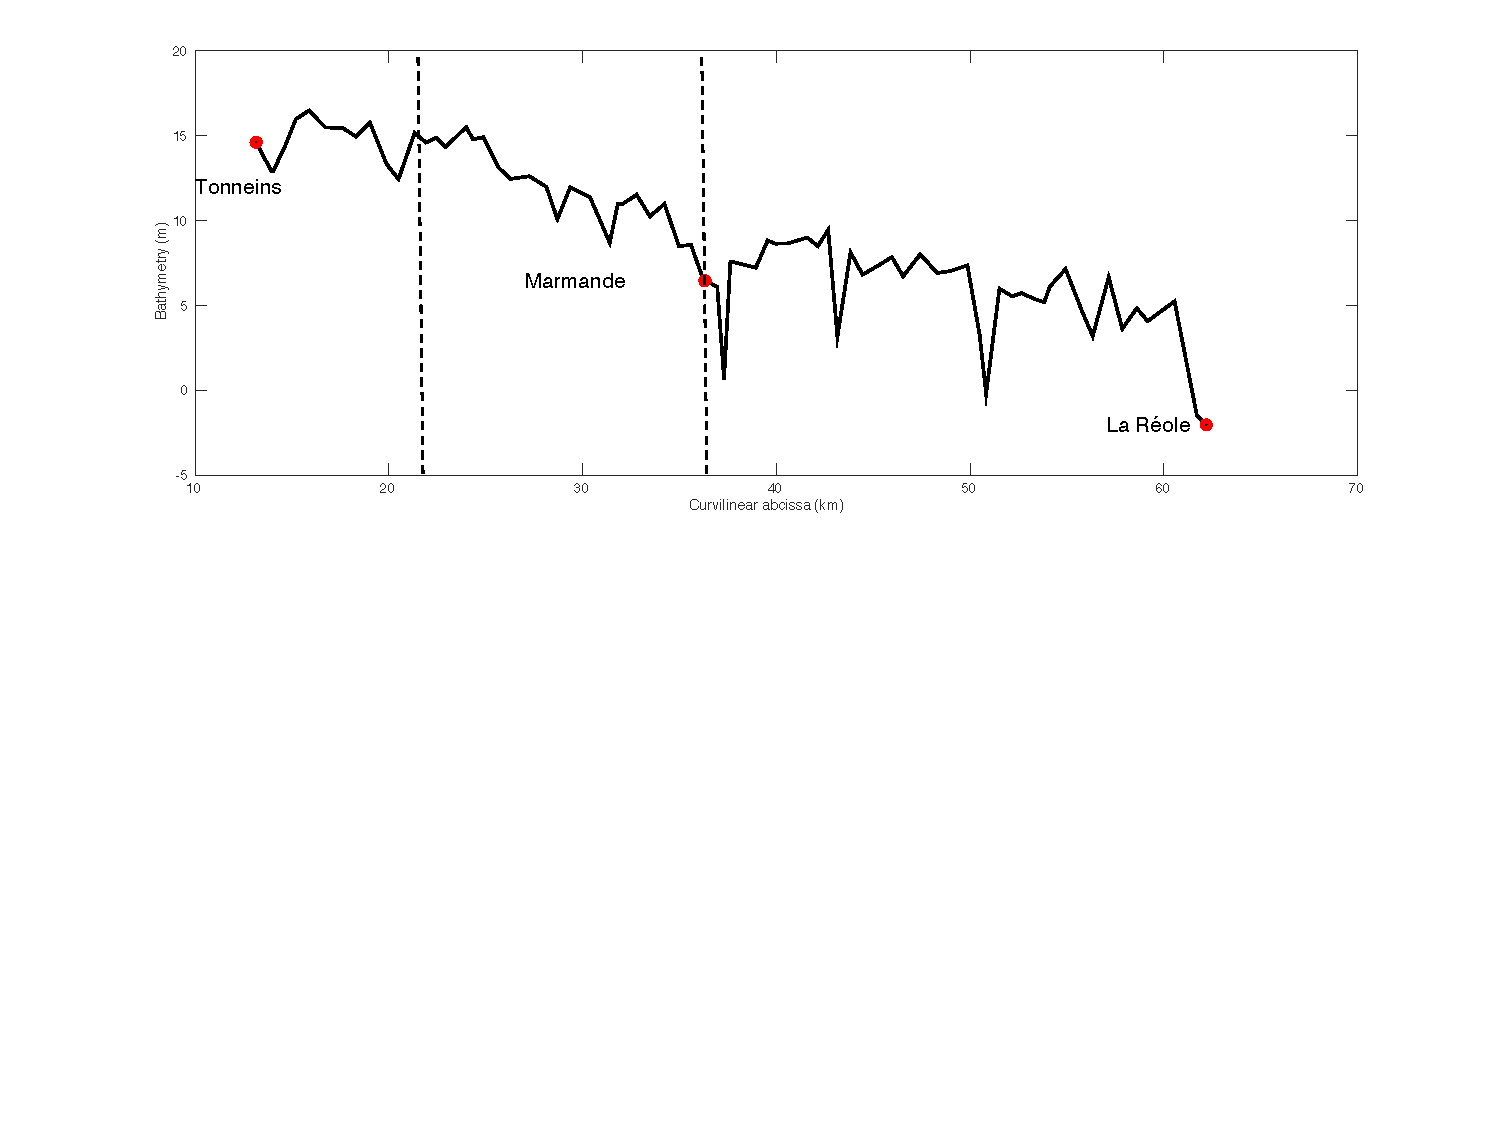
\includegraphics[width=0.9\linewidth,height=\textheight,keepaspectratio]{fig/applications/mascaret/Fig1b.pdf}}
\caption{Garonne River case study (South-West France). (a)~Reach between Tonneins (upstream, $a_{\text{in}} = 13$~km) and La Réole (downstream, $a_{\text{out}} = 62$~km) with Marmande located at $a = 36$~km. (b)~Bathymetry profile along the curvilinear abscissa $a$~(km) between Tonneins and La Réole. The Strickler friction coefficient $K_s$ spatially varies as a constant piecewise function; the changes in the value of $K_s$ are indicated by vertical dashed lines.}
\label{fig:garonne}
\end{figure}

The upstream steady boundary condition is prescribed by $Q(a_{\text{in}}) = Q_{\text{in}}$; the discharge $Q$ is constant along the reach ($Q = Q_{\text{in}}$). The downstream boundary condition is prescribed with a local rating curve $RC$ established at La R\'eole that sets $h(a_{\text{out}}) = RC(Q_{\text{out}}) = h_{\text{out}}$. The hydraulic model has been calibrated using channel and floodplain roughness coefficients as free parameters~\citep{besnard2011}. 

\subsection{Sources of uncertainties and Quantity of Interest}\label{sec:database}

UQ and DA for flood forecasting are essential to ensure the predictive capability of the surrogate model at the observing stations such as Marmande. Previous work~\citep{elmocaydEMA} has shown that in steady state conditions and given some assumptions on the statistics of the input uncertain variables, the sensitivity of the hydraulic state at Marmande to $K_{s_3}$ is predominant; the sensitivity at Marmande to $K_{s_1}$ and $K_{s_2}$ is null because of the steady state assumption and given the present hydraulic model. Hence, the main sources of uncertainties taken into account here are the upstream mass flow rate $Q$ and the Strickler coefficient $K_{s_3}$. We denote by $\mathbf{x} = (Q, K_{s_3})$ the random vector of size $d = 2$. From expert knowledge, $Q$ and $K_{s_3}$ are considered as independent random variables. $Q$~(m$^3$\,s$^{-1}$) follows the normal distribution $\mathcal{N}(4031,400)$: the mean is set to the average flow in the Garonne River; the standard deviation (STD) is chosen in order to remain in subcritical flow. $K_{s_3}$~(m$^{1/3}$\,s$^{-1}$) follows the uniform distribution $\mathcal{U}(15,60)$: the range of the uniform distribution is chosen following calibration results. This range for the variables $Q$ and $K_{s_3}$ allows to test how the surrogates are affected by non-linearities. 

MASCARET provides as output the water height over 463 cross-sections for the Garonne case. In this work, we focus on the water height at $M = 14$ stations evenly distributed along the 50-km reach, among which Marmande at $a = 36$~km. Even though the surrogate models are formulated with respect to the predominant uncertain variables for water level at Marmande and downstream, the surrogates are computed over the entire network. On this hydraulic network, in-situ observations are only available at Marmande and the improvement of the water level at Marmande and downstream of Marmande
relies on the improvement of $Q$ and $K_{s_3}$ only. Yet, the correlation function between the water level error at Marmande and the other locations is needed in the DA algorithm. We denote by $\mathbf{h}$ the vector of $M$ observed water levels for one realization of MASCARET.

A database noted $\mathcal{D}_{N_{\text{ref}}}$ and containing $N_{\text{ref}} = \numprint{100,000}$ MASCARET simulations was compiled as a reference for the study. Each simulation corresponds to a different pair of inputs ($Q, K_{s_3}$) resulting from a MC random sampling following $Q\sim\mathcal{N}(4031,400)$ and $K_{s_3} \sim \mathcal{U}(15,60)$. In the present study, $D_{N_{\text{ref}}}$ is partly used to build the PC and GP surrogates via the training set 
$\mathcal{D}_N = (\mathcal{X}$, $\mathcal{Y})\subset \mathcal{D}_{N_{\text{ref}}}$ of size $N$; it is fully used to validate them a posteriori over a large ensemble (\cref{sec:validation}).


\section{Comparison of Polynomial Chaos (PC) and Gaussian Process (pGP) surrogates}\label{sec:UQresults}

\subsection{Reference Monte Carlo (MC) results}
\label{sec:UQresults_ref}

We first present the results obtained using the MC reference sampling ($N_{\text{ref}} = 100,000$ in $\mathcal{D}_{N_{\text{ref}}}$) in terms of water level mean, STD, PDF, correlation matrix as well as Sobol' indices associated with $Q$ and $K_{s_3}$. These results are used as reference to evaluate the accuracy of the PC and pGP surrogate models.

\Cref{fig:monte-carlo_pdf}a displays the water level PDF computed from $\mathcal{D}_{N_{\text{ref}}}$ data set integrated with a MC approach for the $M = 14$ stations along the curvilinear abscissa $a \in [a_{\text{in}}, a_{\text{out}}]$. The mean water level (\cref{ref:mean_mc}) is represented with a thick black line; the interval between two STD (Eq.~\ref{ref:std_mc}) is represented with dotted lines; and the minimum and maximum water level values are represented with dashed lines. In steady state, water level of the upstream part is mostly sensitive to $Q$. The dispersion of the ensemble is thus mostly driven by the dispersion of $Q$. At the very downstream part of the river ($a=60$~km), the dynamics is driven by the downstream boundary condition where the water level and discharge are related by the local rating curve $RC$. The water level is a function only of discharge and the roughness coefficient has no influence; thus the spread of the ensemble tends to decrease near the downstream boundary condition. After Marmande, the flow is driven both by $K_{s_3}$ and $Q$, the dispersion of the ensemble is larger than upstream of Marmande. At Marmande ($a = 36$~km), the flow is complex due to strong variation of the local bathymetry (\cref{fig:garonne}b), the ensemble spread is larger and the PDF plotted in~\cref{fig:monte-carlo_pdf}b features two main modes due to the change in backwater curves solutions for subcritical flow.
 
\begin{figure*}[!h]               
\centering
\subfloat[Along the 50 km reach.]{
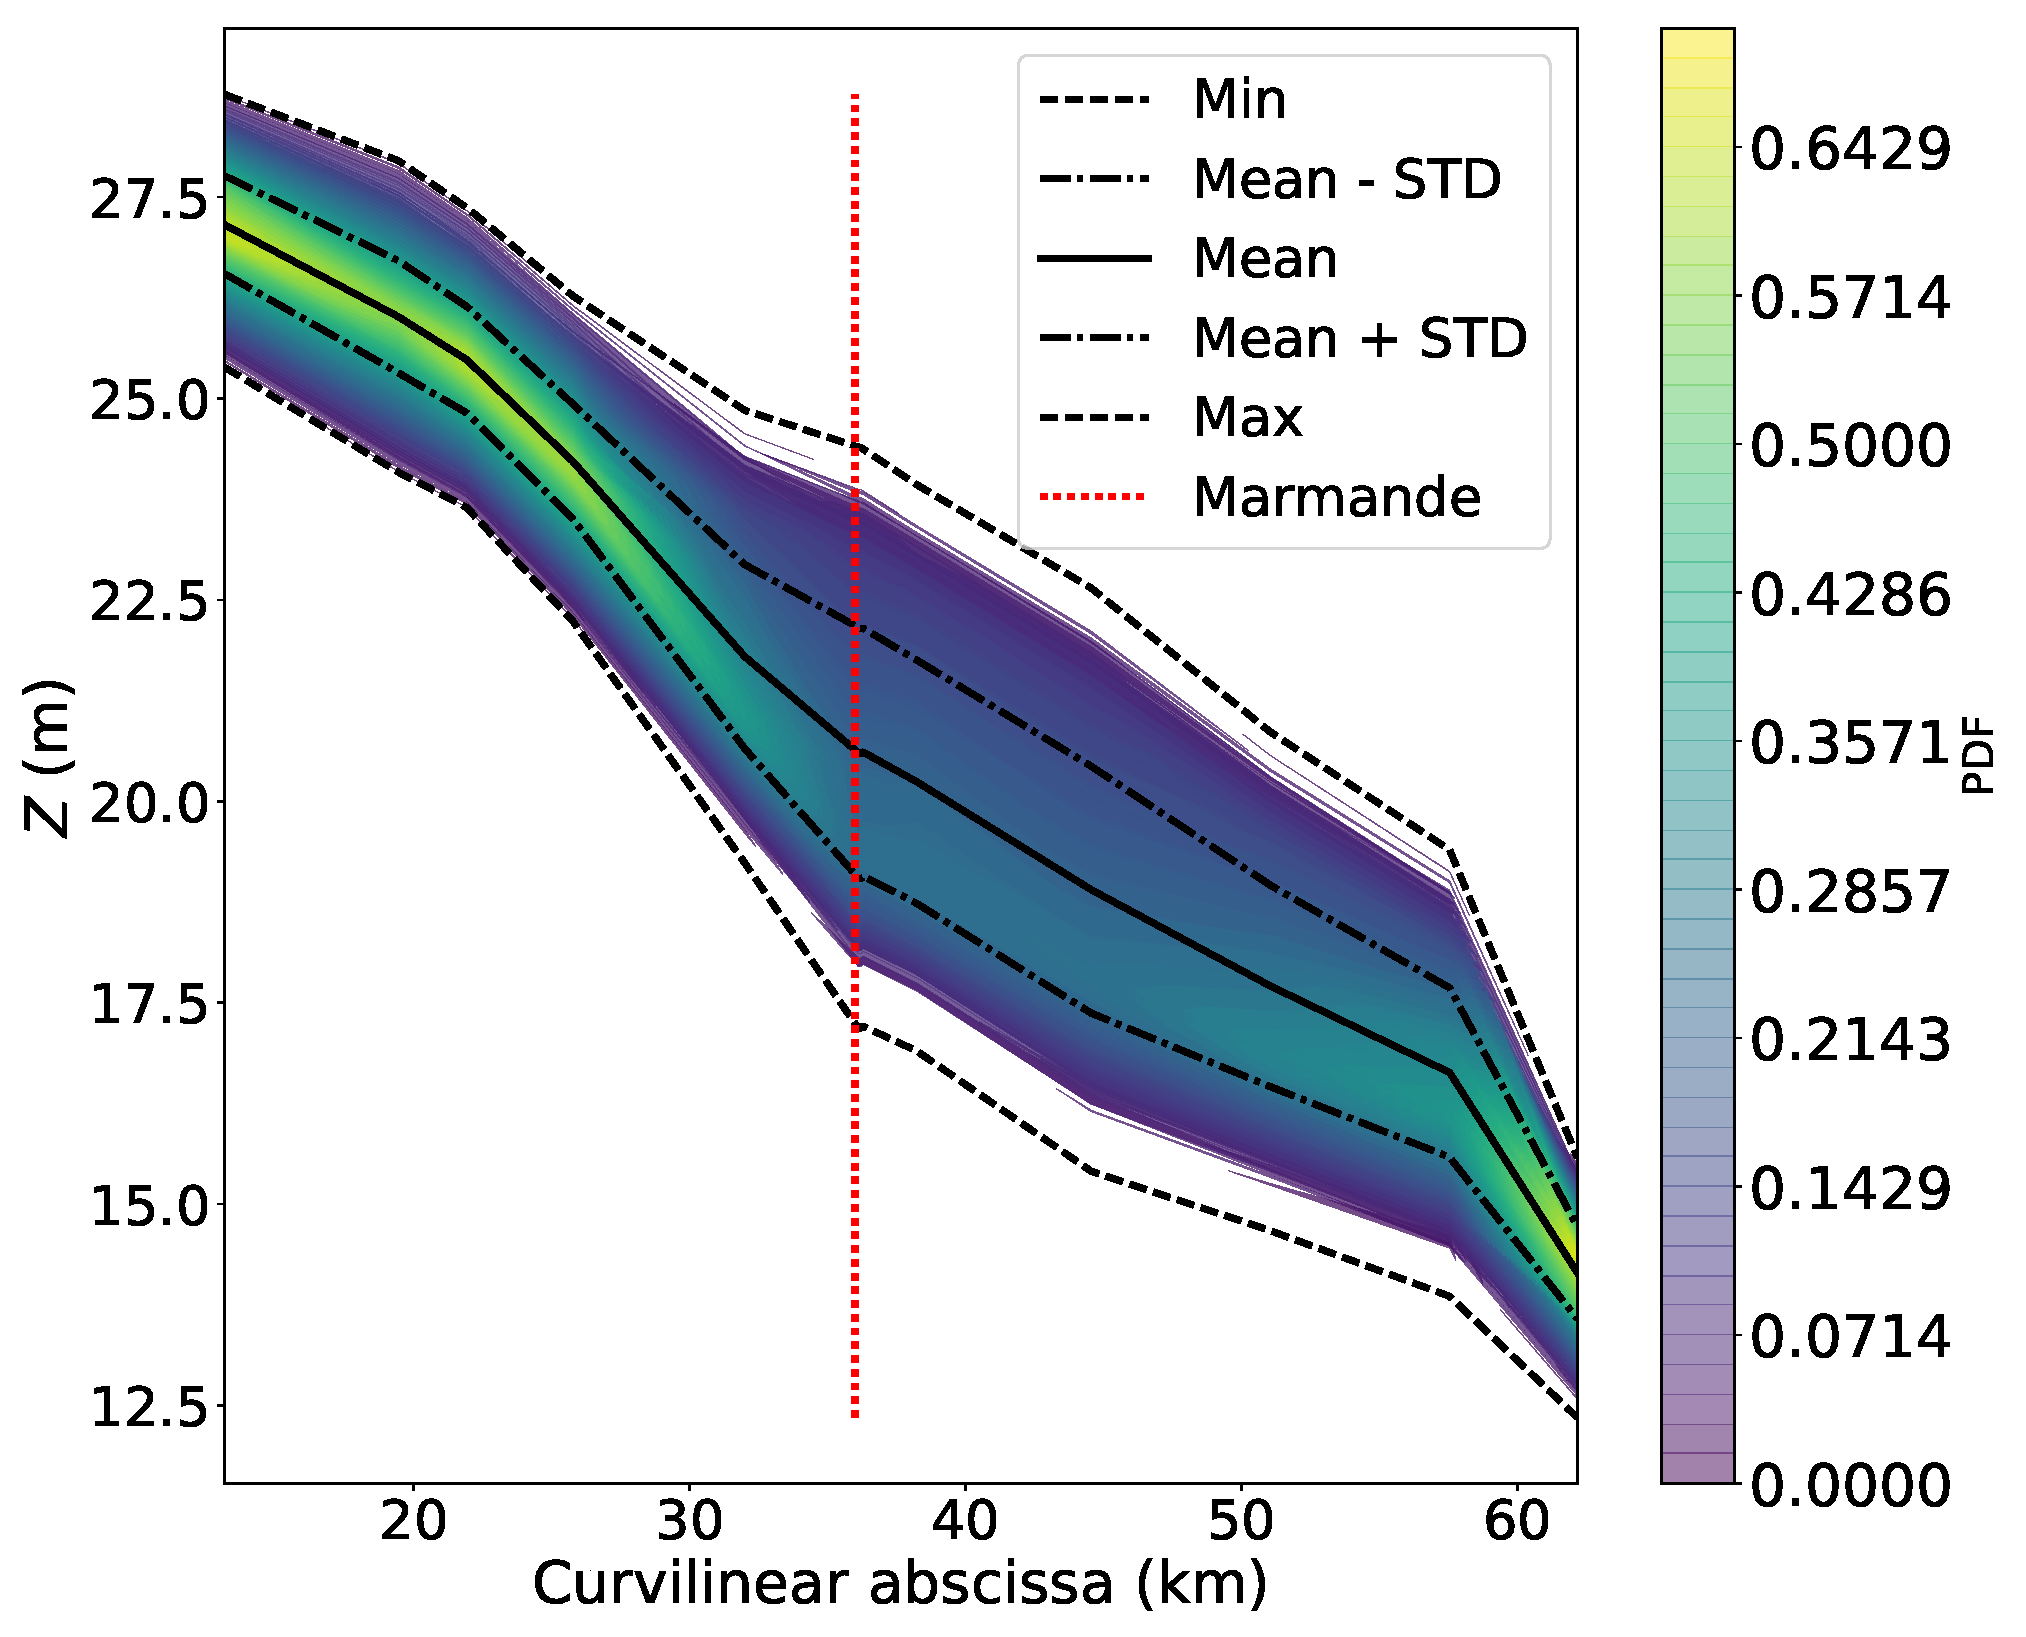
\includegraphics[width=0.47\linewidth,height=\textheight,keepaspectratio]{fig/applications/mascaret/Fig2a.pdf}} 
\subfloat[At Marmande ($a = 36$~km).]{
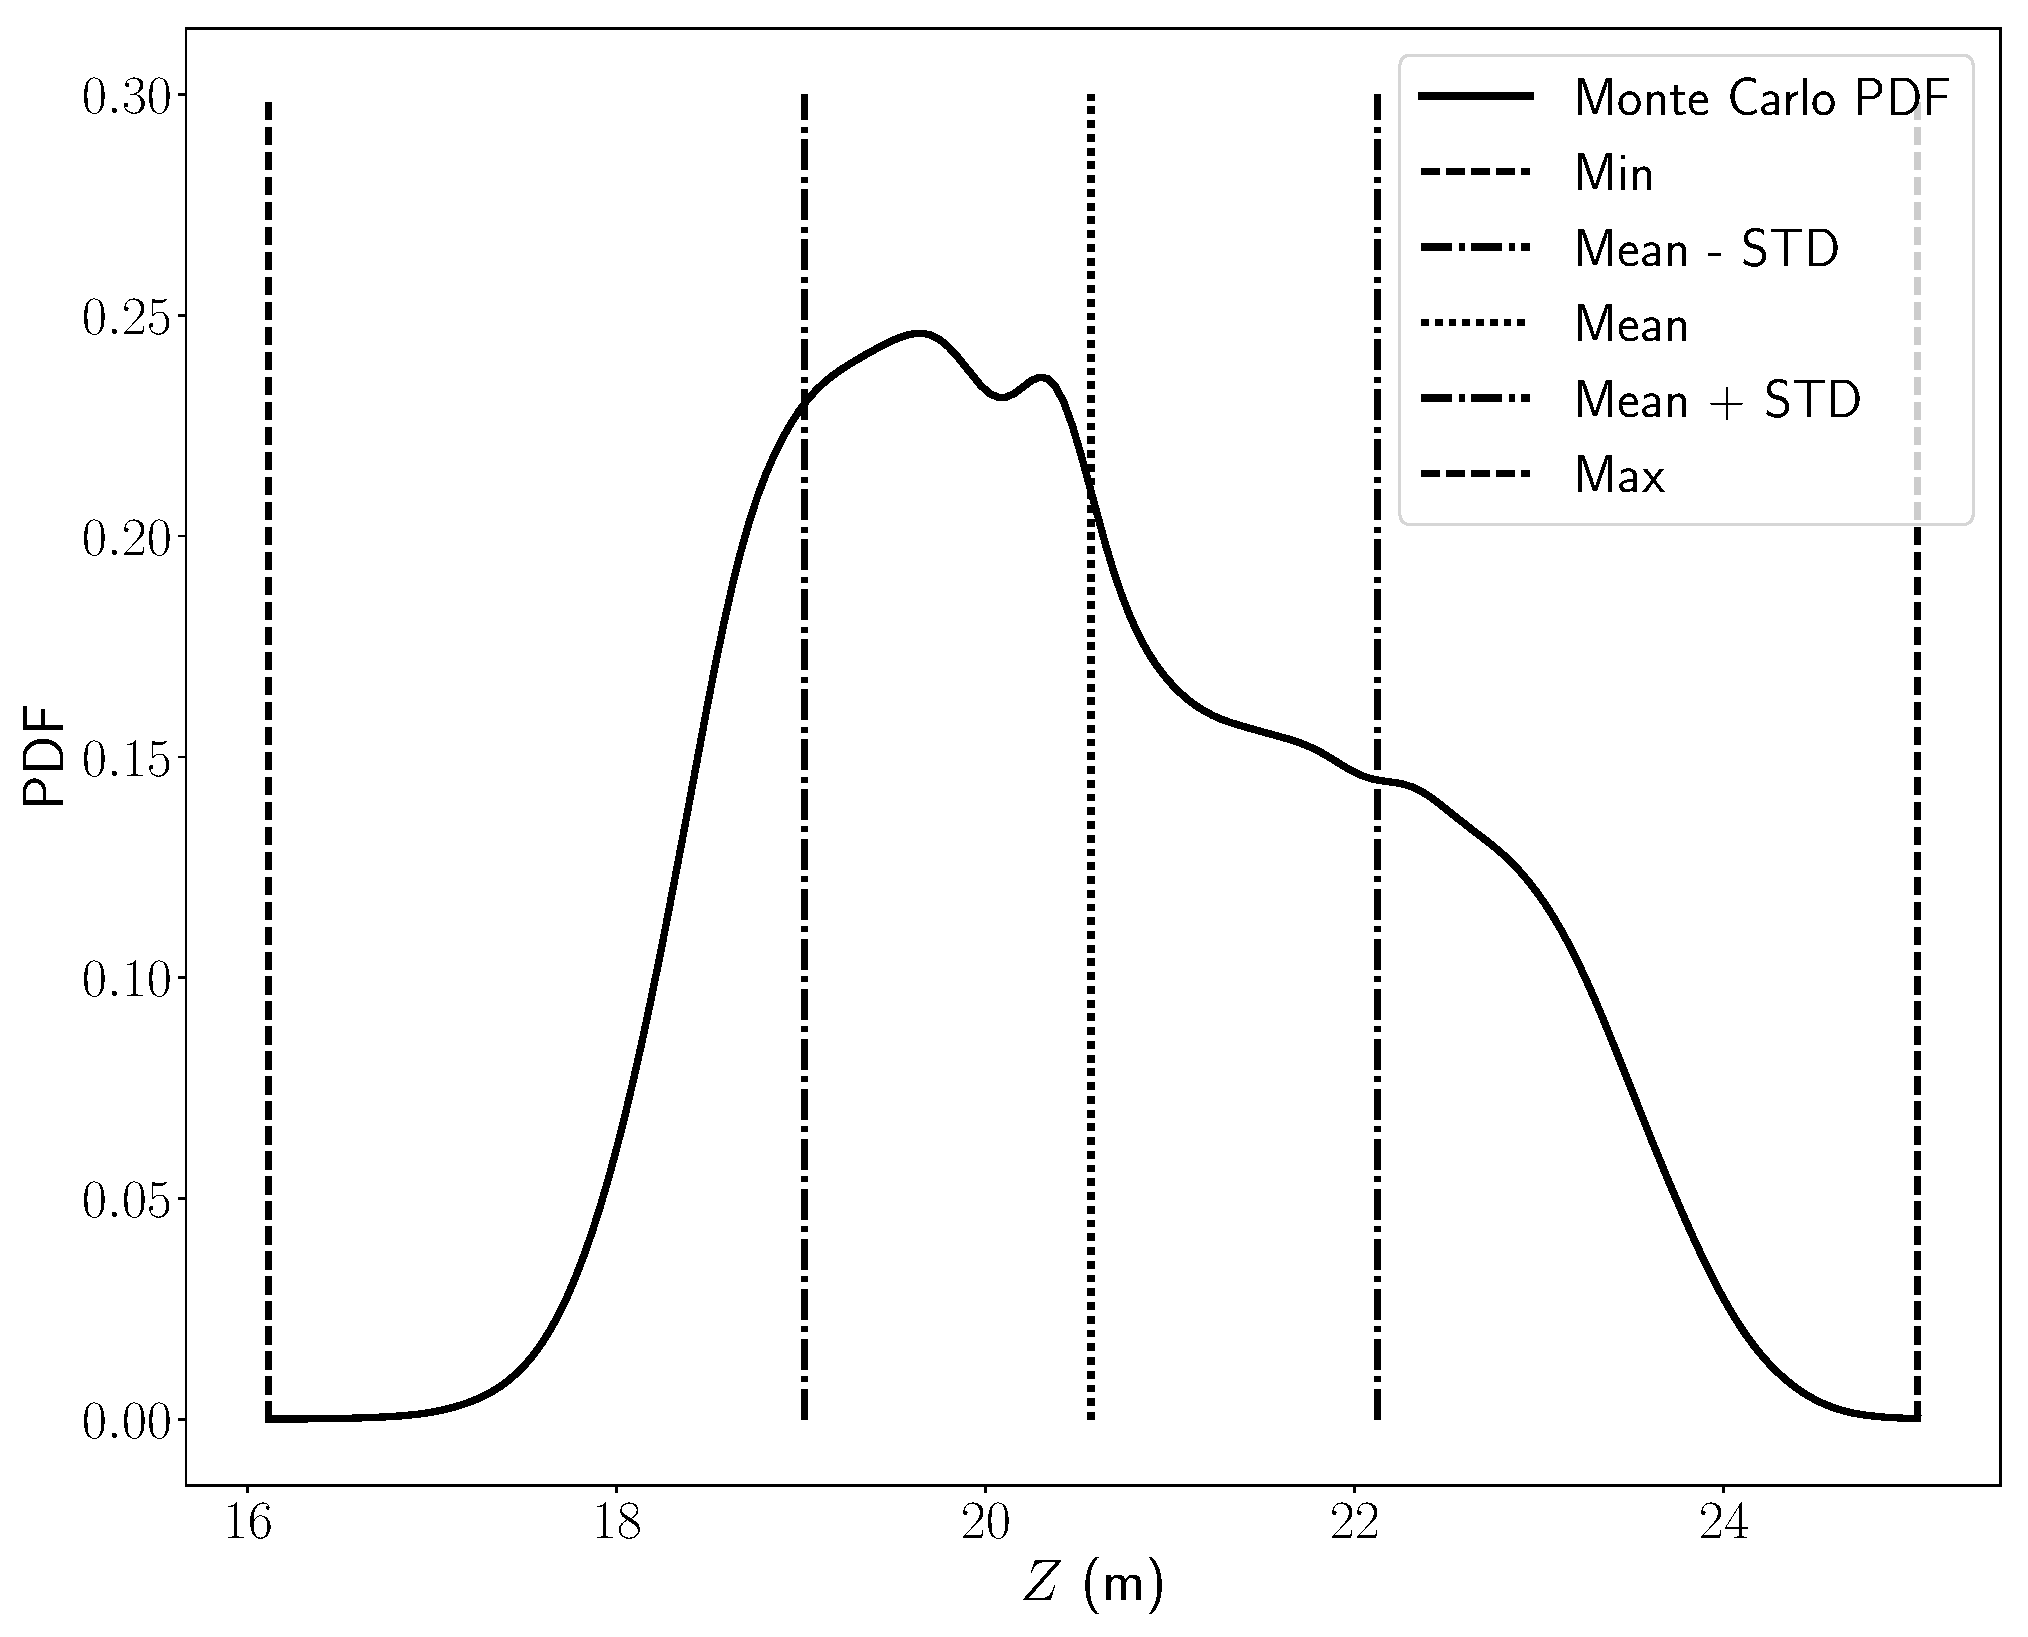
\includegraphics[width=0.47\linewidth,height=\textheight,keepaspectratio]{fig/applications/mascaret/Fig2b.pdf}}
\caption{Reference PDF of the water elevation obtained with the $N_{\text{ref}} = 100,000$ snapshots in $\mathcal{D}_{N_{\text{ref}}}$ derived from MC random sampling: (a)~at the $M = 14$ stations along the 50 km river reach; (b)~at Marmande. The solid line indicates the mean water level with respect to the curvilinear abscissa; the dotted lines indicate the spread corresponding to 2~STD; the dashed lines indicate the maximum and minimum water level values; and the vertical dotted line indicates Marmande's location.}
\label{fig:monte-carlo_pdf}
\end{figure*}

The Sobol' indices for the water level $S_Q$ and $S_{K_{s_3}}$ computed from $\mathcal{D}_{N_{\text{ref}}}$ with respect to $Q$ and $K_{s_3}$ are presented in~\cref{fig:monte-carlo_sobol_corr}a along the curvilinear abscissa $a$. These indices confirm the previously mentioned spatial sensitivity. The water level variance is mostly explained by the upstream discharge variability for $a = [0; 30~\text{km}]$---the variability of $K_{s_3}$ has a small impact in the upstream part of the river in steady state conditions. It is then mostly explained by the Strickler coefficient variance for $a = [30; 60~\text{km}]$. Near the downstream boundary condition, the water level is related to the discharge by the local rating curve $RC$, the very last part of the network is thus under the influence of the discharge. First and total order indices are almost equal, meaning that the correlation between the variability in the input parameters is weak. One should keep in mind that these observations are the results of the PDFs and hydraulic regime assumptions that were made.

\Cref{fig:monte-carlo_sobol_corr}b displays the water level correlation matrix along the 50 km reach (derived using~\cref{eq:cov_mc}) that is estimated from $\mathcal{D}_{N_{\text{ref}}}$. The $n$th column of the matrix describes the water level error correlations between one given location on the channel $a_n$ and the rest of the channel $a_m$ with $a_m \in [a_{\text{in}}, a_{\text{out}}]$. By definition, the correlation is equal to 1 on the diagonal, it decreases when the distance between $a_n$ and $a_m$ increases. We first analyse the correlation function for a point located upstream of the river ($a_i = 15~\text{km}$) where $S_Q = 0.9$ and $S_{K_{s_3}}= 0.1$. Water level errors are strongly correlated in the upstream part of the river, which is under the influence of the upstream discharge boundary condition, where $S_Q$ is large. Errors between $a = 15$~km and the rest of the river tends to decorrelate when the influence of $K_{s_3}$ increases (i.e.~where $S_{K_{s_3}}$ is larger). We then analyse the correlation function for Marmande ($a = 36~\text{km}$) where $S_Q= 0.15$ and $S_{K_{s_3}}= 0.85$. The correlation between water level errors at Marmande and the rest of the river is large in the vicinity of Marmande, where the influence of $K_{s_3}$ prevails. It then decreases for upstream and downstream locations that are under the influence of the upstream discharge and the downstream rating curve $RC$ (where $S_Q$ is large), respectively.
\begin{figure*}[!h]               
\centering
\subfloat[]{
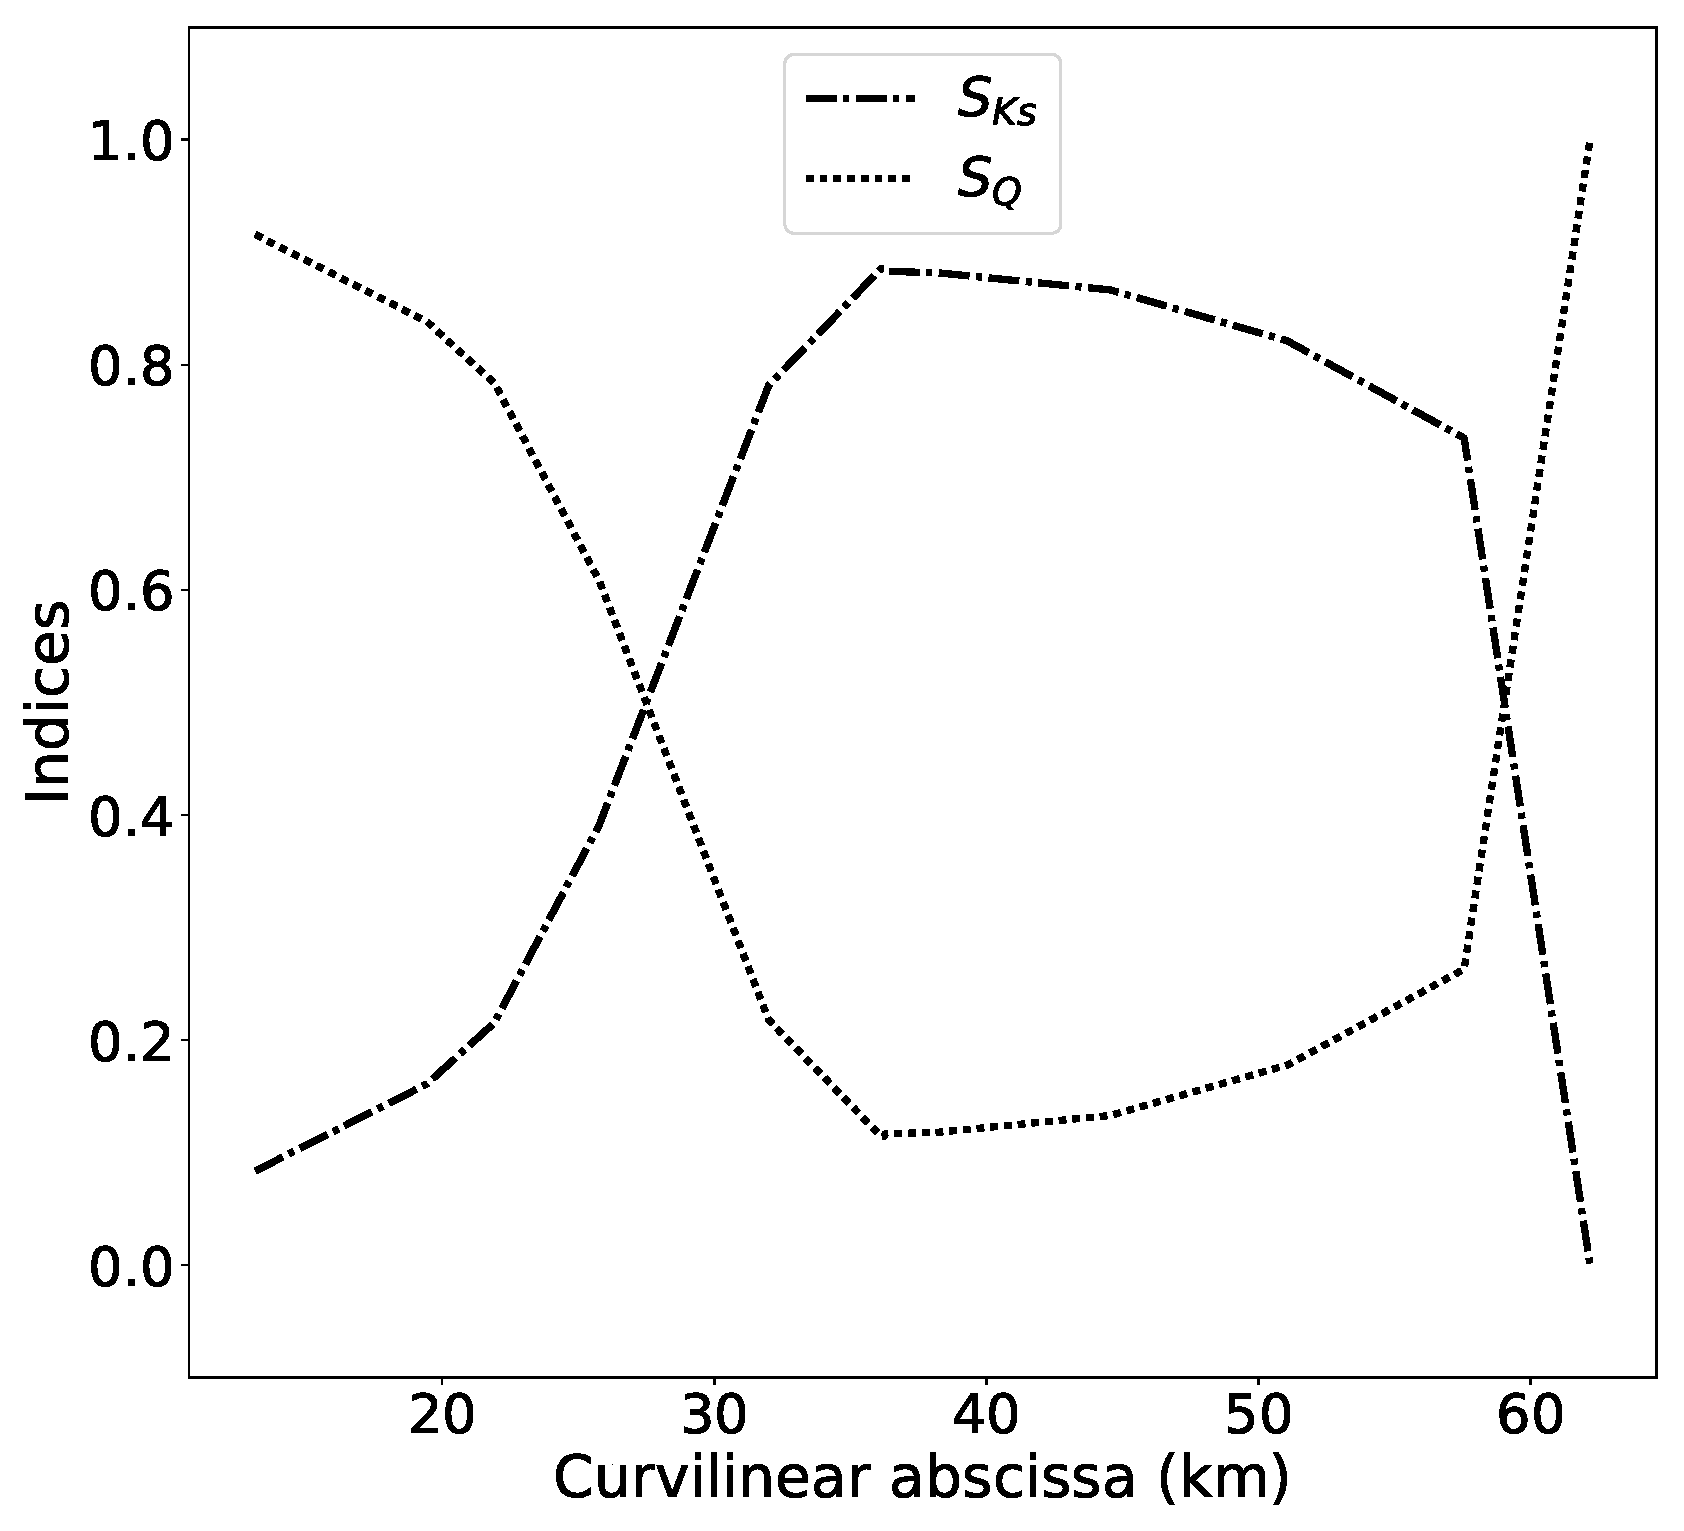
\includegraphics[width=0.45\linewidth,height=\textheight,keepaspectratio]{fig/applications/mascaret/Fig3a.pdf}} 
\subfloat[]{
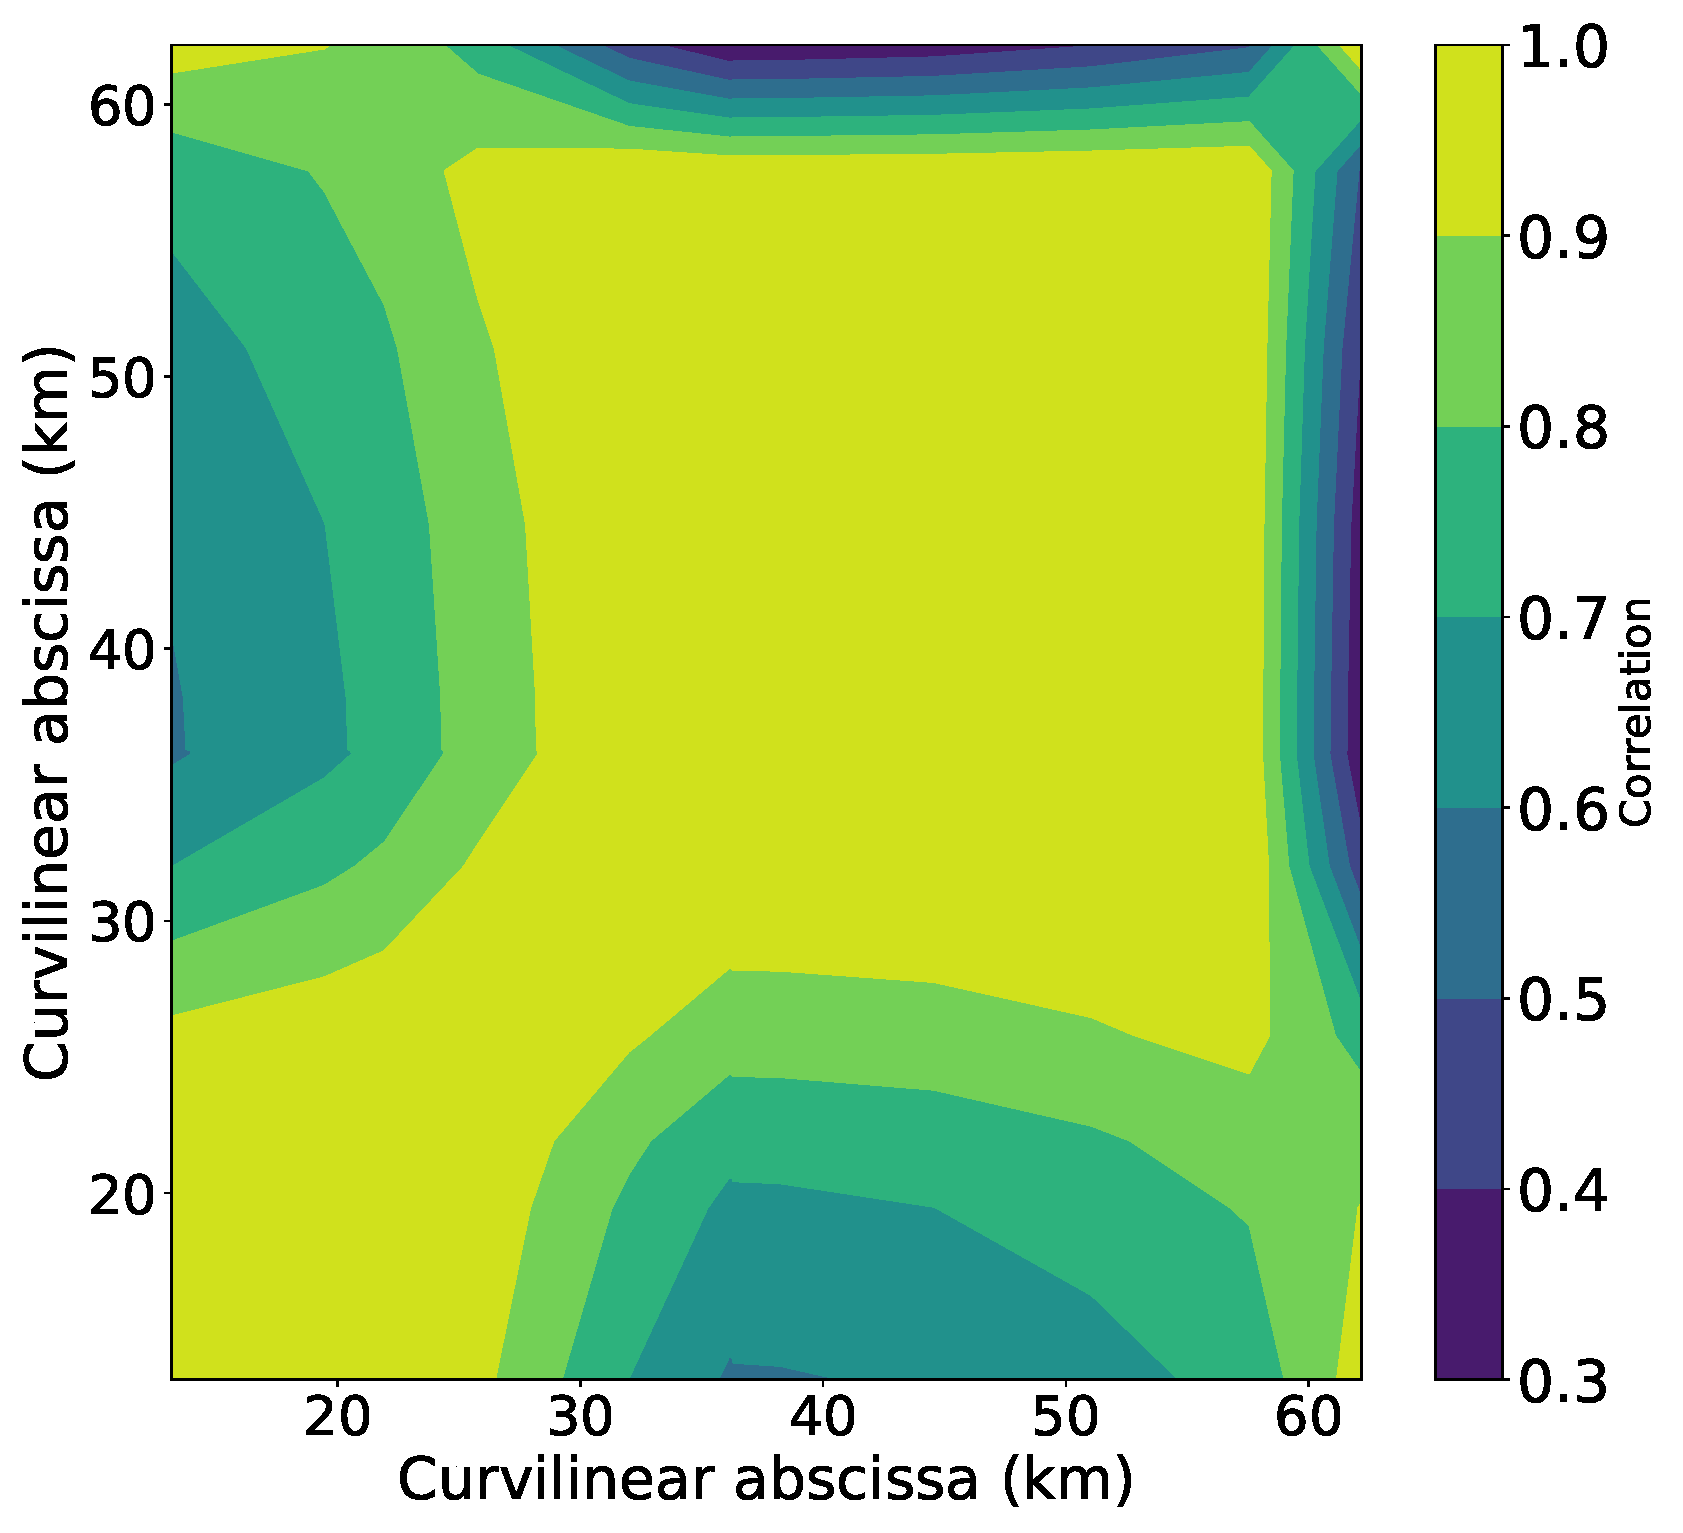
\includegraphics[width=0.45\linewidth,height=\textheight,keepaspectratio]{fig/applications/mascaret/Fig3b.pdf}}
\caption{Measures of importance using MC random sampling. (a)~Reference Sobol' first order indices along the 50 km reach. Dashed-dotted line corresponds to the Sobol' index associated with the Strickler coefficient $K_{s_3}$. Dotted line corresponds to that associated with the upstream discharge $Q$. (b)~Reference spatial correlation matrix $\mathbf{C}_{\text{mc}}$ associated with the spatially distributed water level $\mathbf{h}$.}
\label{fig:monte-carlo_sobol_corr}
\end{figure*}

\subsection{Convergence Analysis for Surrogates}

We now use the same metrics as for the MC random sampling approach in~\cref{sec:UQresults_ref} to evaluate the accuracy of both PC and pGP surrogates. The surrogate models are built using a training set $(\mathcal{X}, \mathcal{Y})$ of size $N$ that is much smaller than that of the reference sample $N_{\text{ref}}$; they are then validated with respect to the reference MC results. The PC surrogate is built using a Gaussian quadrature rule with $N = (P+1)^2$ particles in the training set ($P$ is the total polynomial degree to be determined). The pGP approach is built using an approximate low-discrepancy Halton's sequence of the same budget as for the PC approach. This is approximate in the sense that we consider the closest values to the standard Halton's sequence that are part of the data set $\mathcal{D}_{N_{\text{ref}}}$. The sensitivity to the value of $P$ and thus to the size of the training set $N$ is investigated.

Both surrogates are computed with a fixed budget $N$ of 49, 121 and 256 MASCARET evaluations. For PC, this value of $N$ corresponds respectively to $P = 6$, $P = 10$ and $P = 15$. The pGP and PC response surfaces at Marmande are presented in~\cref{fig:response-surface-pgp-pc} for $N = 49$ and $N = 121$. The design of experiment is represented by black dots. The colour map is evaluated by sampling each surrogate over the full data set $\mathcal{D}_{N_{\text{ref}}}$ made of $N_{\text{ref}} = 100,000$ particles. It is found that the water level increases with increasing discharge $Q$ and decreasing Strickler coefficient $K_{s_3}$, consistently with MASCARET behaviour. Due to the quadrature rule, increasing the number of snapshots (from $P = 6$ in~\cref{fig:response-surface-pgp-pc}c to $P = 10$ in~\cref{fig:response-surface-pgp-pc}d) allows to build a higher order PC surrogate valid on a wider input range for $Q$ that is described by a Gaussian PDF. For $P = 10$, some of the quadrature roots are outside of the MC sample and require additional MASCARET evaluations to build the PC surrogate $\mathcal{M}_{\text{pc}}$. Looking at the pGP design of experiments, the input space interval for $Q$ has been arbitrarily fixed to optimally represent the PDF. Since we consider a Gaussian distribution, its range has been bounded to $[3000;5000~\unit{m^3\,s^{-1}}]$. Following Chebyshev's theorem, this leads to a~90~\% confidence interval.

The distribution of the particles in the design of experiments used by PC and pGP differs. This is done on purpose based on previous performance tests carried out with respect to the training set size $N$ and evaluating the surrogate accuracy, see~\cite{elmocaydEMA} and~\cite{roy2016}, respectively. On the one hand, the design of experiments for the PC surrogate is constrained by the PDF of the uncertain inputs. We use here a quadrature-based PC since it was found to be more cost-effective than regression-based PC for a small dimensional problem ($d = 2$) on the Garonne case~\citep{elmocaydEMA}. On the other hand, using the approximate Halton's sequence is known to be accurate for pGP surrogate~\citep{Damblin2013}. This is indeed useful to cover the uncertain space without any bias and to have low discrepancy, meaning that most of the quantity of interest variance is captured and that a good $Q_2$ criterion is achieved. The choice of the design of experiment will be driven in future work according to the study objectives. For instance, DA usually relies on the assumption of Gaussian PDF for the input parameters, so the design of experiments can use this prior information. For risk analysis, threshold values are paramount and a design of experiment accounting for parameter space extrema is required.

\begin{figure}[!h]               
\centering
\subfloat[pGP - 49 snapshots.]{
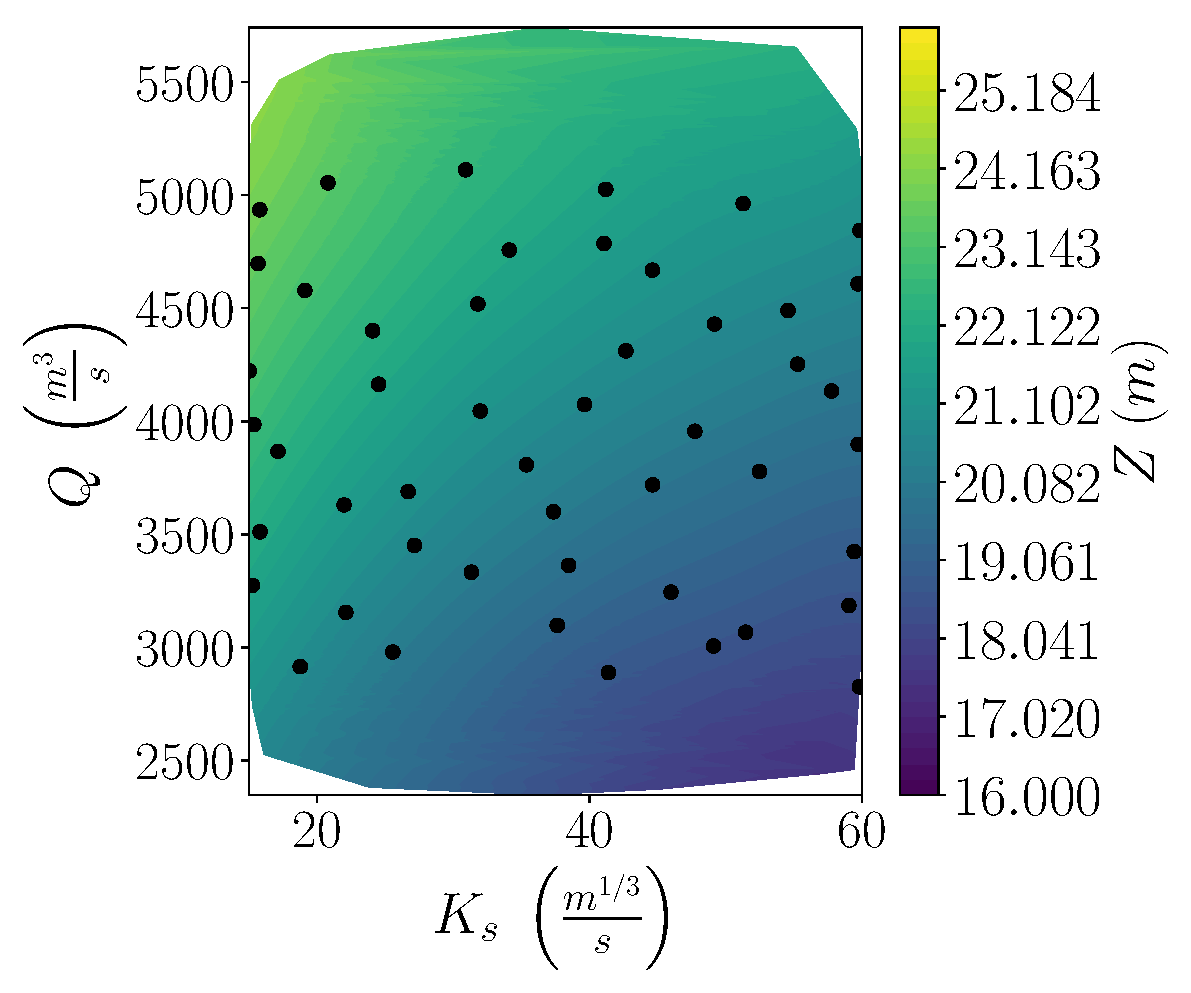
\includegraphics[width=0.47\linewidth,height=\textheight,keepaspectratio]{fig/applications/mascaret/Fig4a.pdf}}          
\subfloat[pGP - 121 snapshots.]{
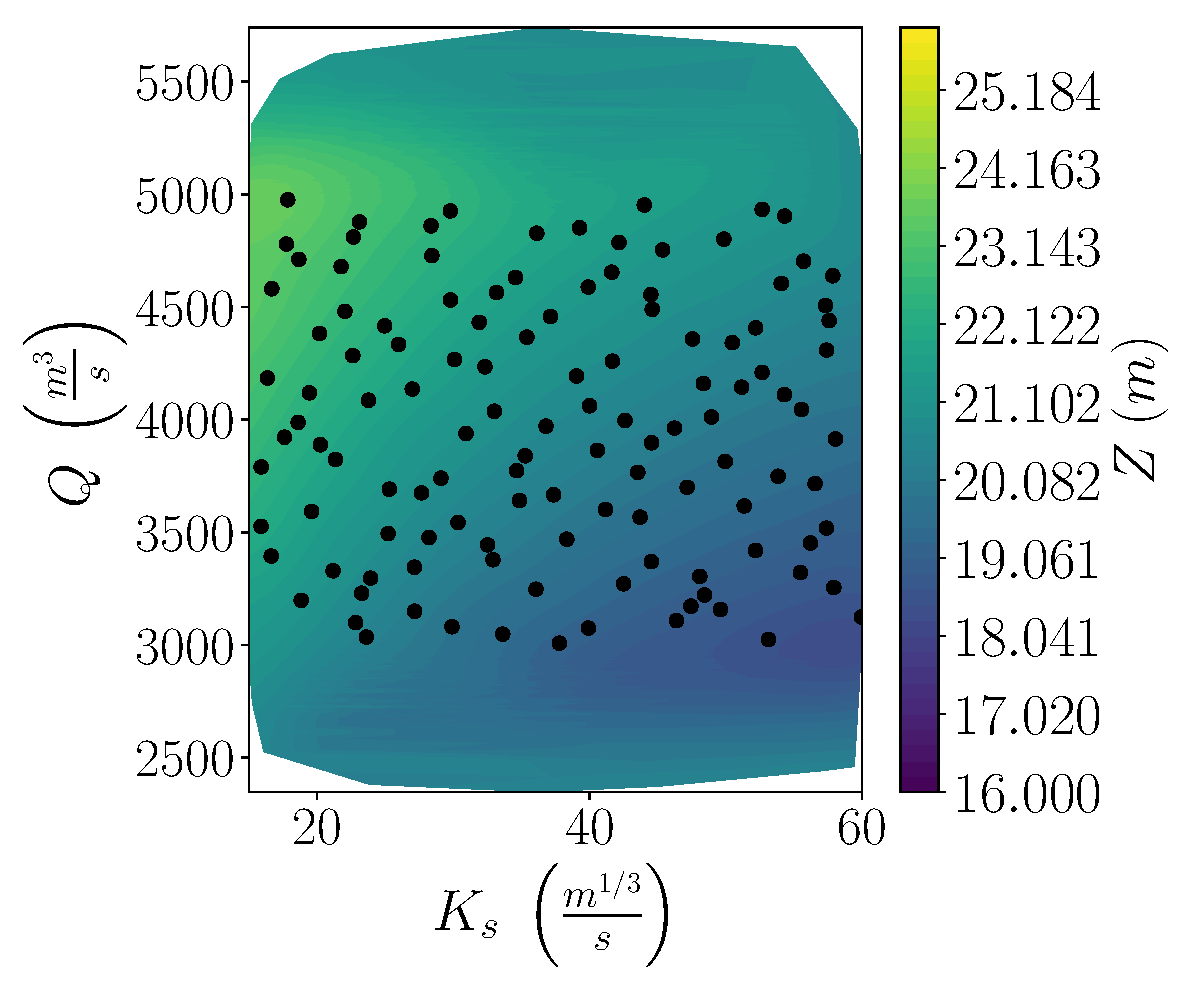
\includegraphics[width=0.47\linewidth,height=\textheight,keepaspectratio]{fig/applications/mascaret/Fig4b.pdf}}

\subfloat[PC - 49 snapshots.]{
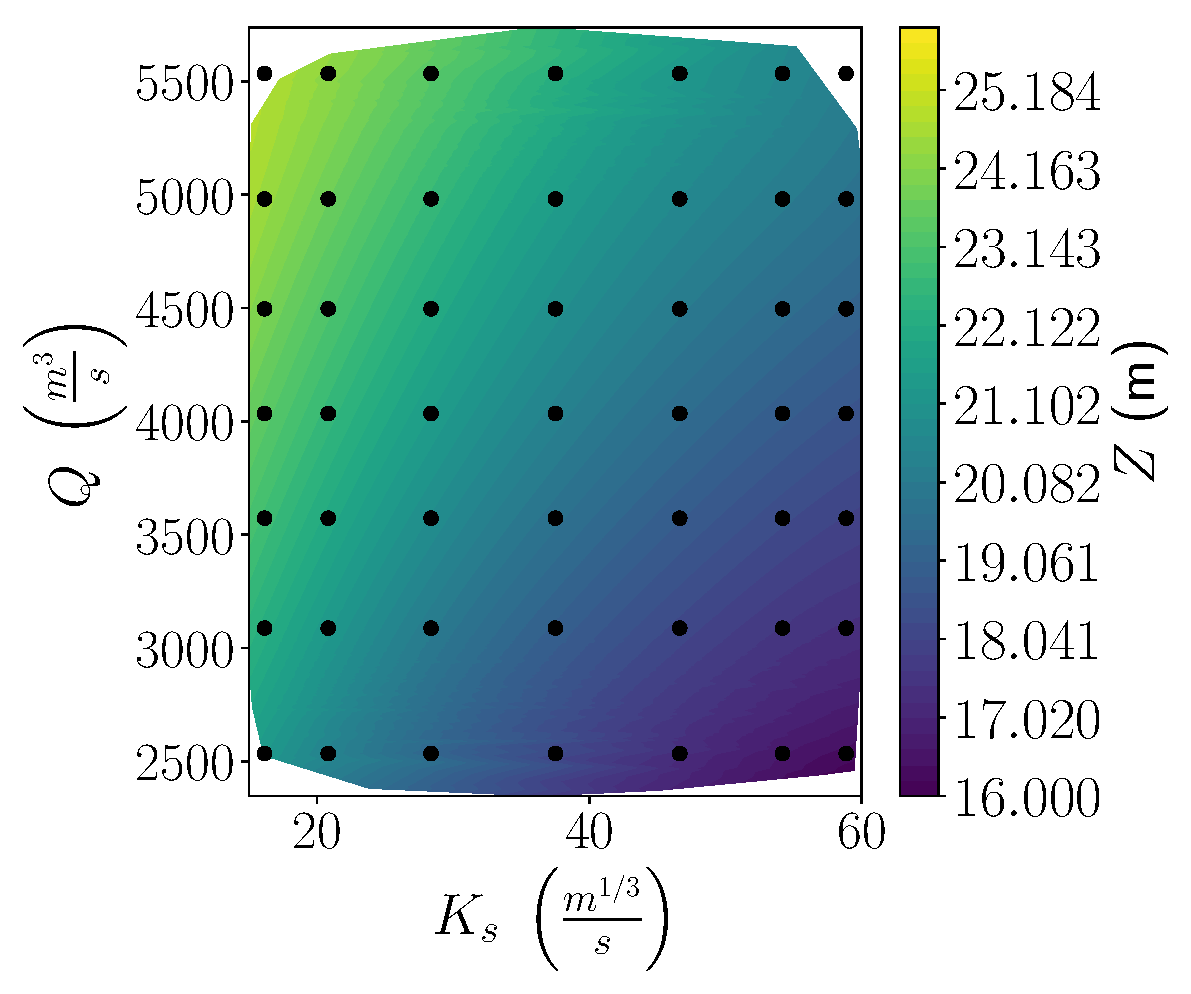
\includegraphics[width=0.47\linewidth,height=\textheight,keepaspectratio]{fig/applications/mascaret/Fig4c.pdf}}           
\subfloat[PC - 121 snapshots.]{
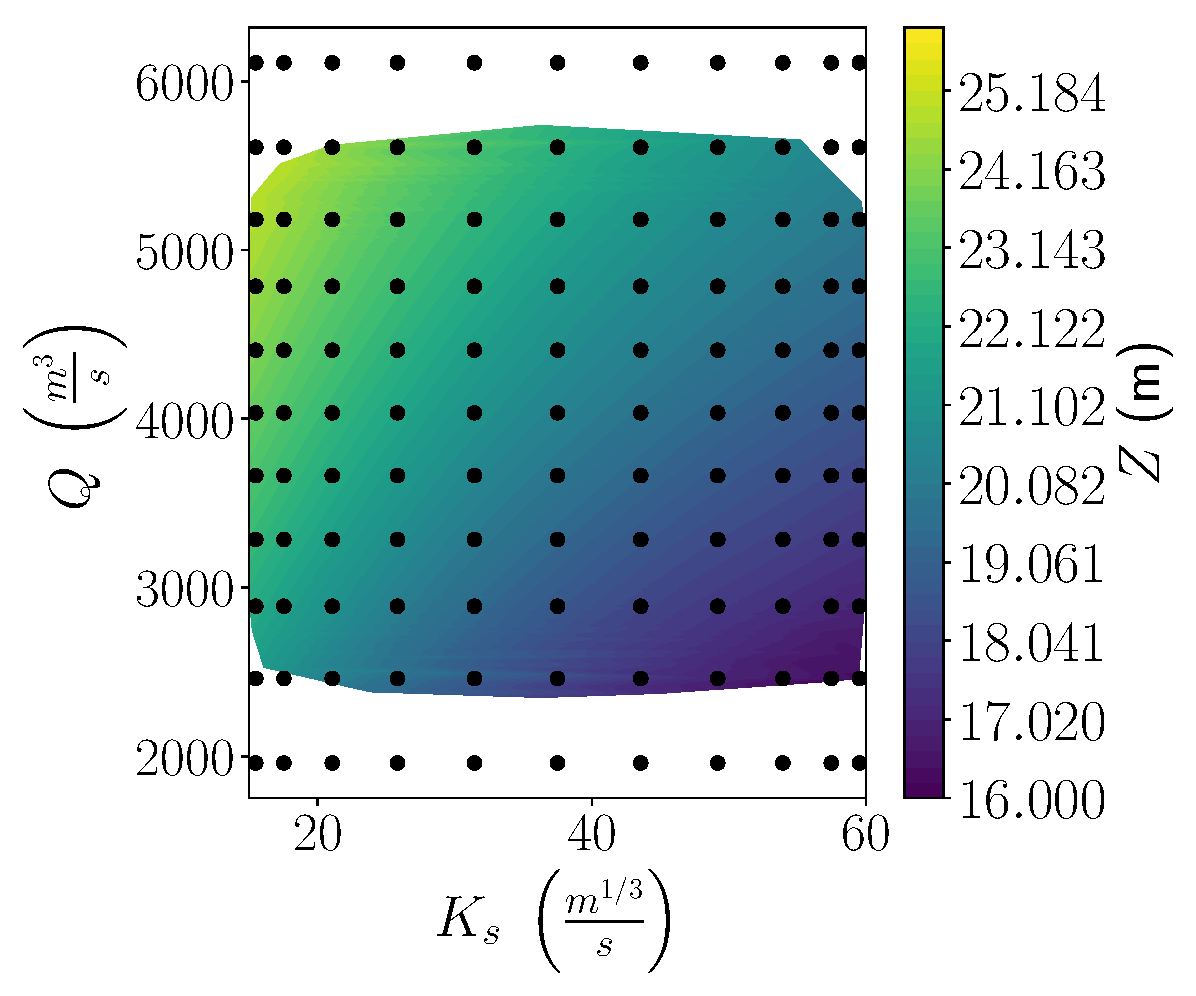
\includegraphics[width=0.47\linewidth,height=\textheight,keepaspectratio]{fig/applications/mascaret/Fig4d.pdf}}
\caption{Water level response surface at Marmande computed at $\mathcal{D}_{N_{\text{ref}}}$. Top: pGP using (a)~$N = 49$ snapshots and (b)~$N = 121$ snapshots. Bottom~: PC using (c)~$N=49$ snapshots and (d)~$N=121$ snapshots. Black dots represent the design of experiments used to construct the surrogate models. The colour map corresponds to the evaluation of the surrogate over the full data set $\mathcal{D}_{N_{\text{ref}}}$.{\color[rgb]{0.9,0.2,0.16}\protect\footnotemark}}
\label{fig:response-surface-pgp-pc}
\end{figure}

\footnotetext{Scaling of (d) was set in order to show the entire design of experiments. This allows to grasp the fact that the parameter space is evaluated in regions that are not evaluated by the MC sampling.}

The $Q_2$ error between the surrogate water level and the forward model water level for $D_{N_{\text{ref}}}$ averaged over the river is given in~\cref{tab:valid_model} for different  sizes of training set $N$ varying between 49 and 256. The error remains below $\numprint{e-3}$, even for $N = 49$ snapshots; it is only slightly improved when the number of snapshots $N$ increases to 256 and beyond. 
\begin{table}[H]
\centering
\caption{$Q_2$ error for pGP and PC surrogates computed with respect to the MC reference. The error corresponds to the average over the $M$ stations with increasing number of snapshots $N$ from 49 to 256.}
\begin{tabular}{lcc}
\toprule
$N$ & pGP & PC \\
\cmidrule{2-3}
49  & 0.99965 & 0.99983\\
121 & 0.99514 & 0.99993\\
256 & 0.99143 & 0.99962\\
\bottomrule
\end{tabular}
\label{tab:valid_model}
\end{table}

The water level PDF estimated with the PC and the pGP surrogate models based on $49, 121, 256$ snapshots are compared in~\cref{fig:pdf-station-0_9} at the curvilinear abscissa $a = 15~\text{km}$ (near upstream boundary condition) and $a = 36~\text{km}$ (Marmande). In the upstream part of the river, the PDF is uni-modal and is well represented with a small number of snapshots for both surrogates. On the contrary, at Marmande, the dynamics of the flow is more complex and the PDF is bimodal. Both PC and pGP surrogates are able to retrieve the overall shape of the PDF at $a = 15~\text{km}$ and $a = 36~\text{km}$. The shape is more accurate when the number of snapshots $N$ increases. This is quantified using a Kolmogorov-Smirnov statistical test, which measures the fit between the water level CDF computed from each surrogate model and that computed from the reference MC.~\cref{tab:ks} indicates that the null hypothesis (\cref{eq:nullhypothesis}) is rejected for both surrogates computed with 49 snapshots (when $D > \numprint{6.082e-3}$) and accepted when at least 121 snapshots are used. For $N = 49$, \cref{fig:pdf-station-0_9}b--d show that the location of the first mode is shifted compared to MC reference. Increasing $N$ to 121 enables the PC approach to correctly locate this mode, while it enables the pGP approach to represent the second mode with an accurate amplitude, leading to an accepted null hypothesis. Each approach presents a particular limitation: the first mode is not well positioned by the pGP approach; the second mode is not captured by the PC approach. As for the tail of the PDF, it is correctly represented by the PC surrogate, while the pGP surrogate slightly oscillates around the shape of the reference MC PDF.

\begin{figure*}[!h]               
\centering
\subfloat[pGP -- $a = 15~\text{km}$]{
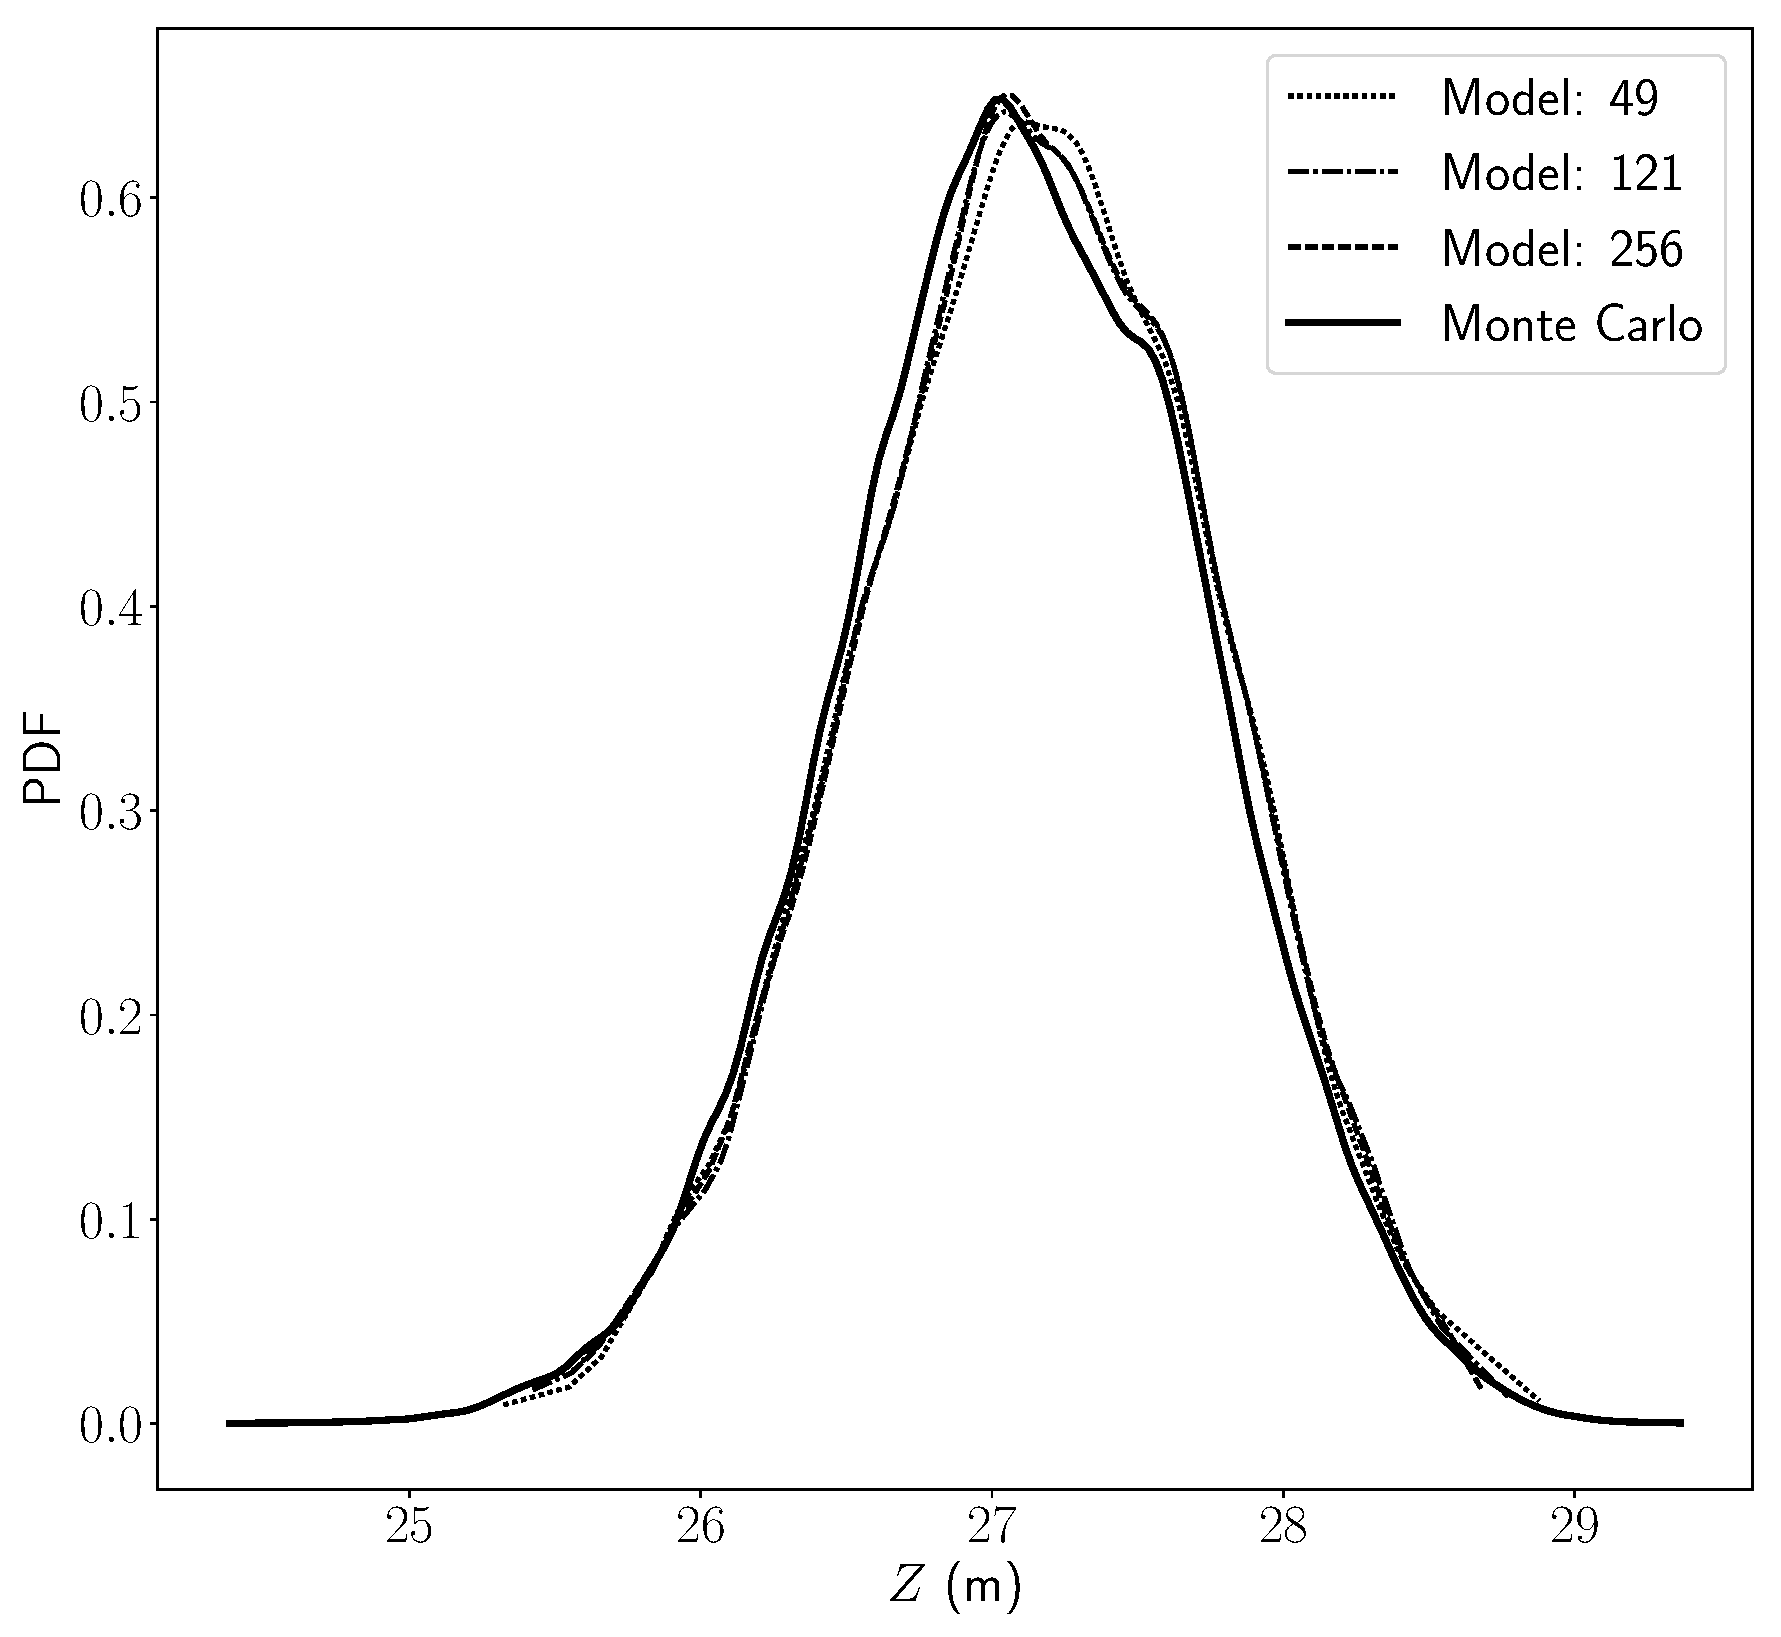
\includegraphics[width=0.47\linewidth,height=\textheight,keepaspectratio]{fig/applications/mascaret/Fig5a.pdf}}
\subfloat[pGP -- $a = 36~\text{km}$]{
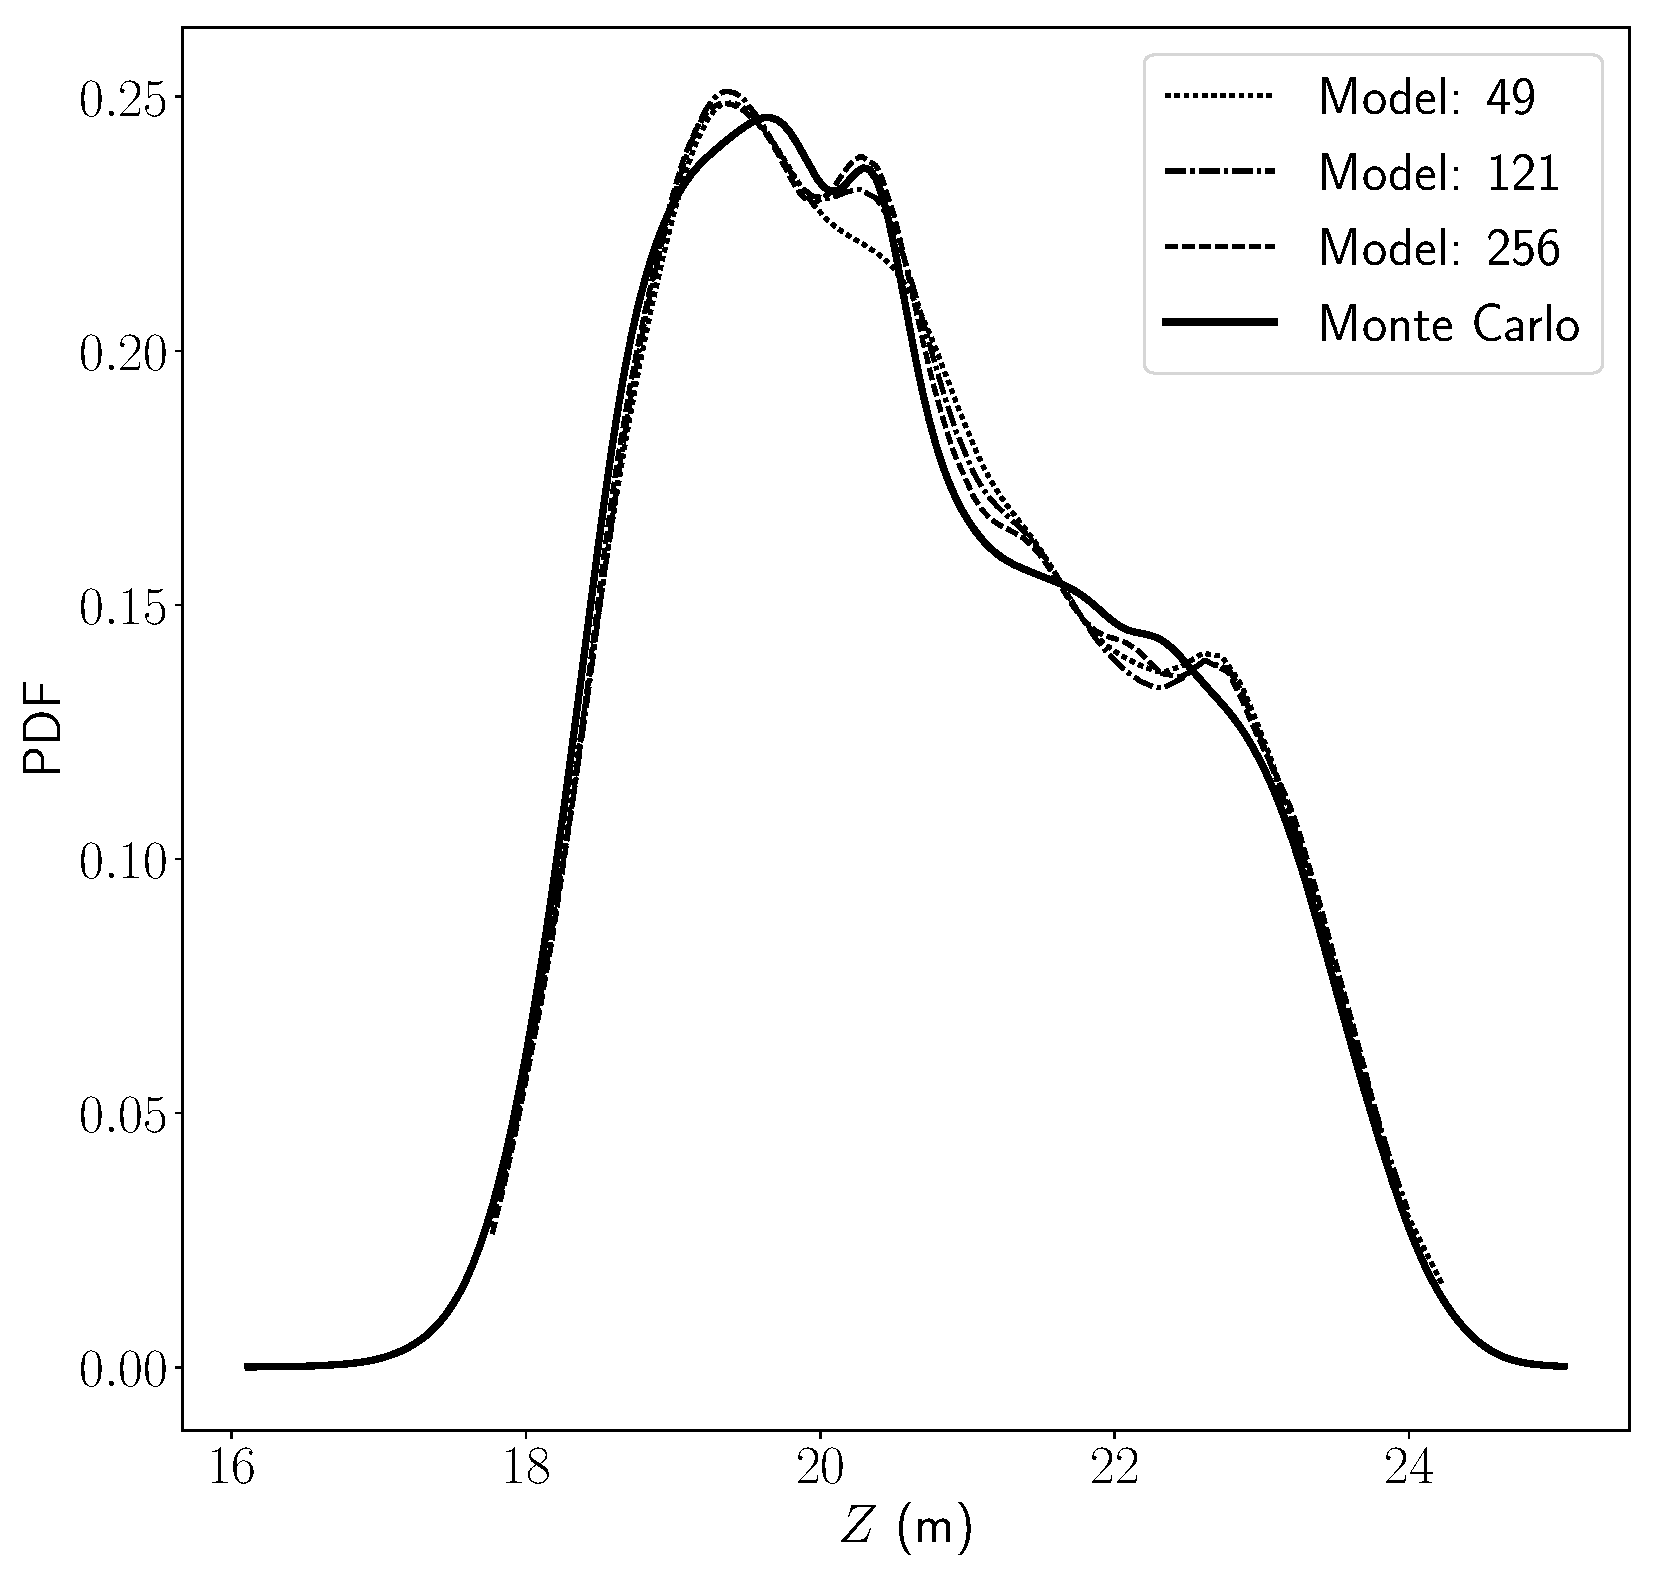
\includegraphics[width=0.47\linewidth,height=\textheight,keepaspectratio]{fig/applications/mascaret/Fig5b.pdf}}

\subfloat[PC -- $a = 15~\text{km}$]{
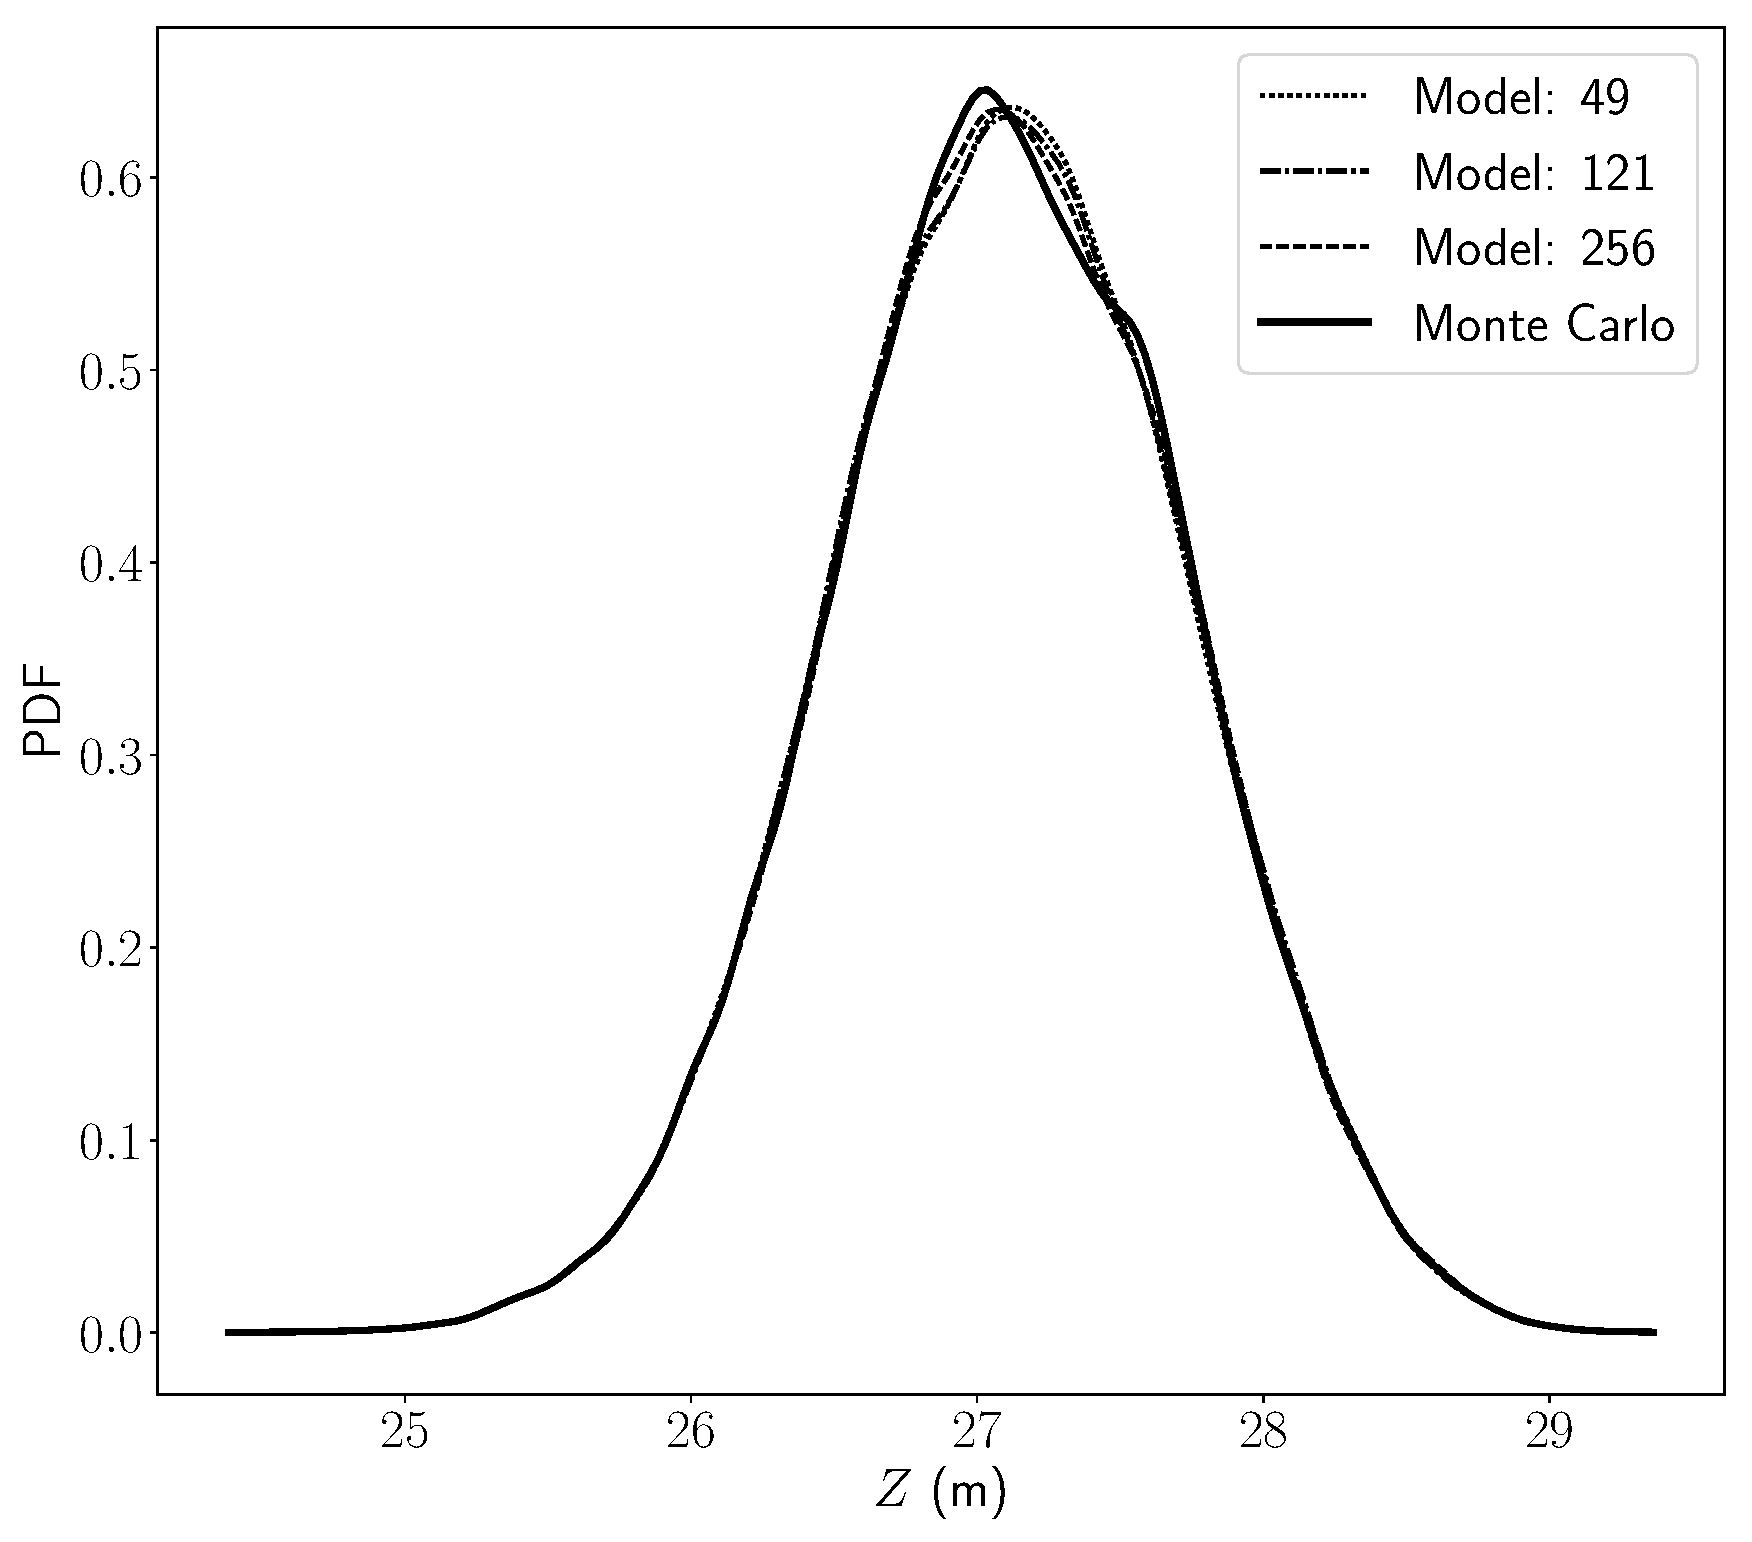
\includegraphics[width=0.47\linewidth,height=\textheight,keepaspectratio]{fig/applications/mascaret/Fig5c.pdf}}
\subfloat[PC -- $a = 36~\text{km}$]{
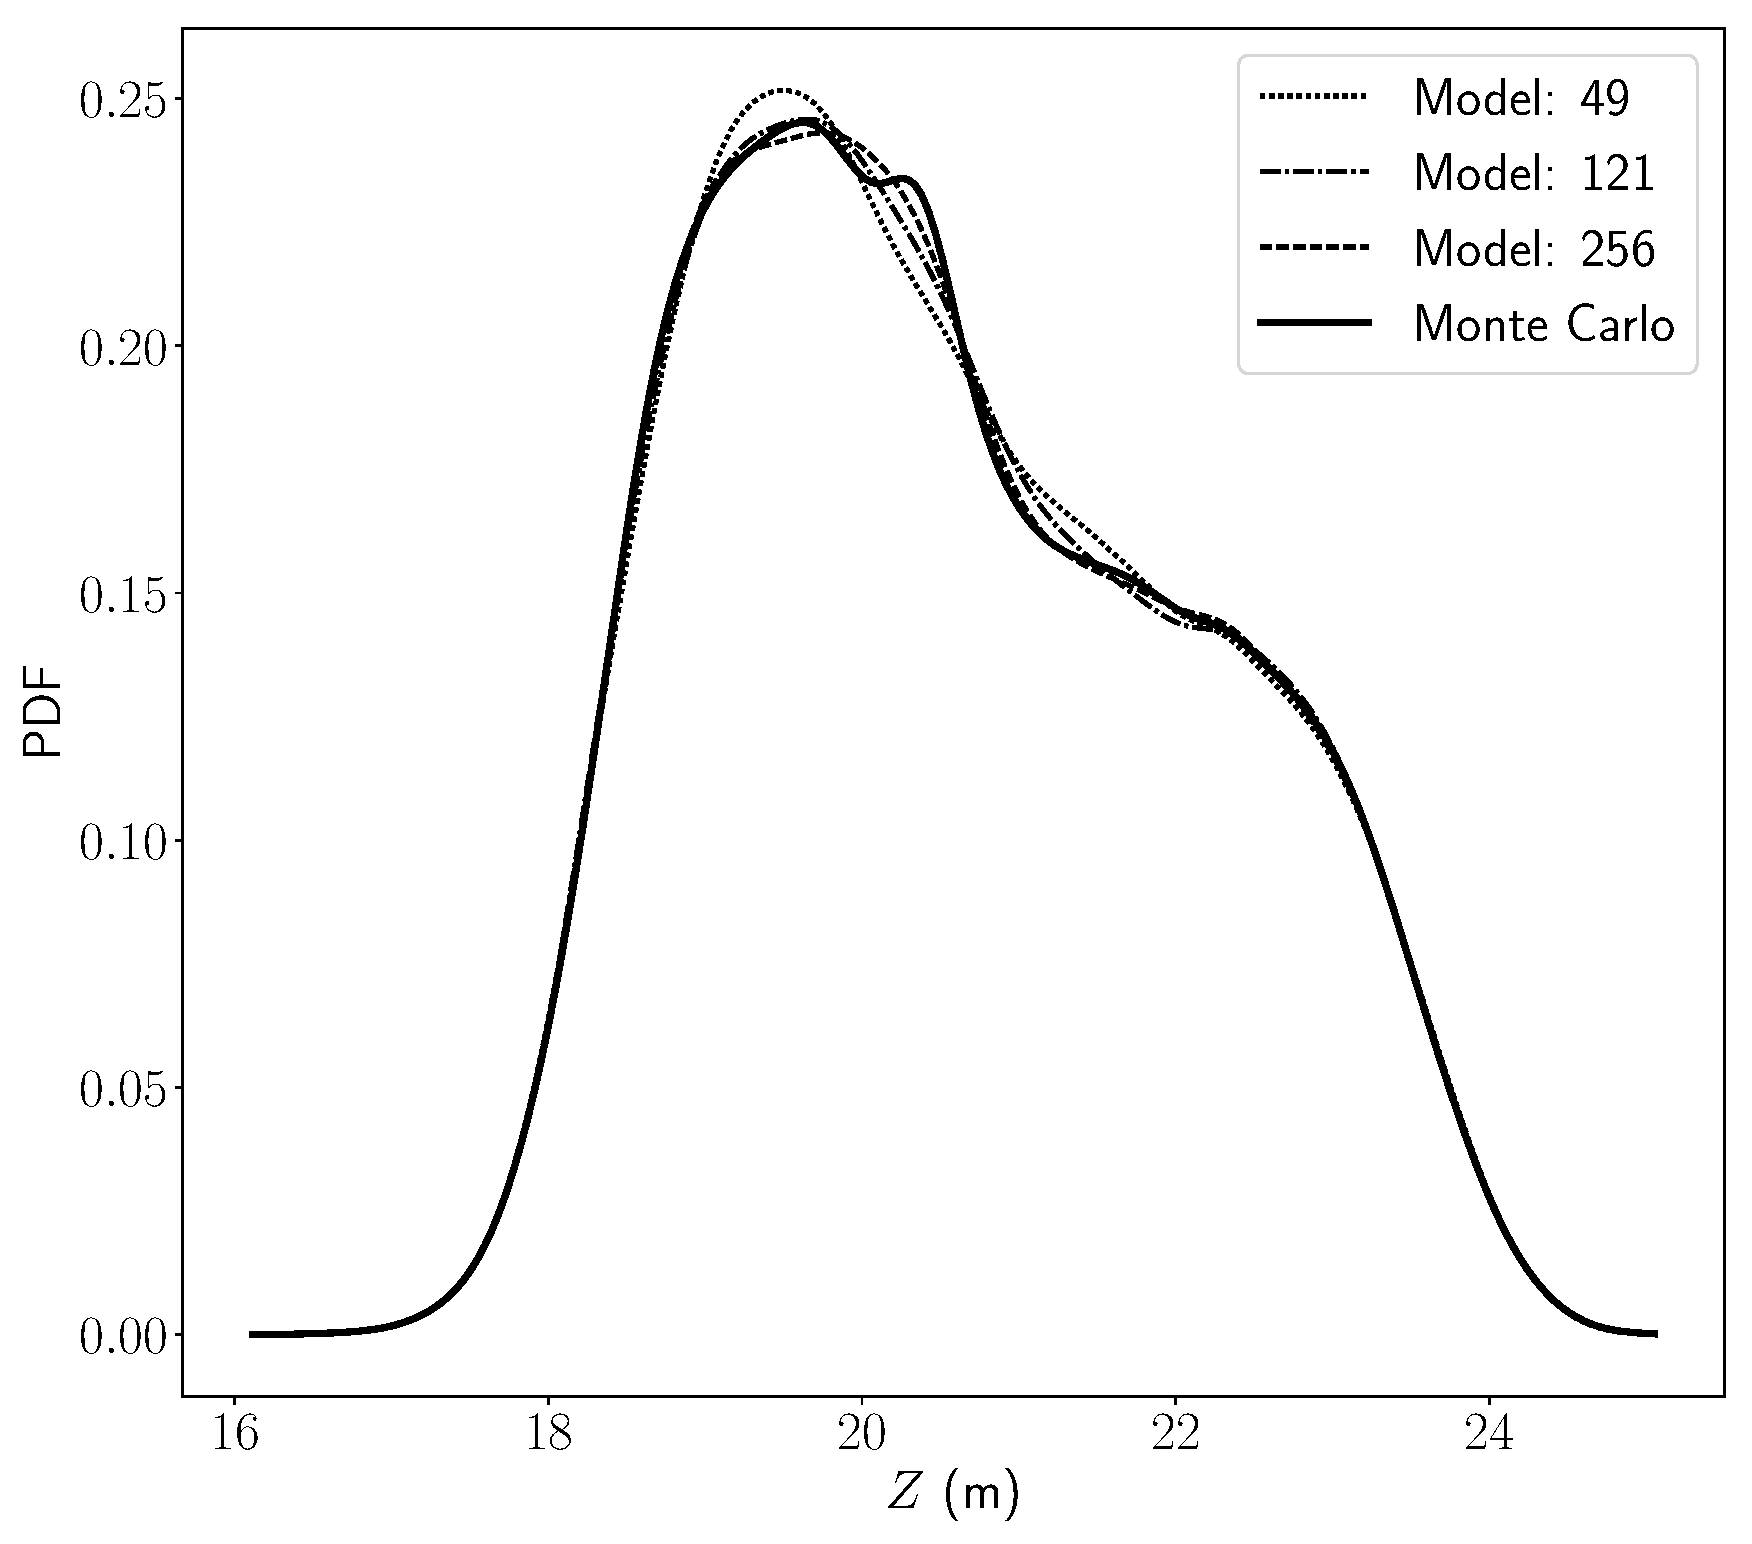
\includegraphics[width=0.47\linewidth,height=\textheight,keepaspectratio]{fig/applications/mascaret/Fig5d.pdf}}
\caption{Comparison of water level PDF obtained with pGP (top panel) and PC (bottom panel) (a)--(c)~At $a = 15~\text{km}$ (near upstream boundary condition). (b)--(d)~At $a=36~\text{km}$ (Marmande). The comparison is carried out for different sizes of training set $N$ (49, 121, 256); the MC result is provided as reference in solid black line.}
\label{fig:pdf-station-0_9}
\end{figure*}

\begin{table}[H]
\centering
\caption{Two-sample Kolmogorov-Smirnov statistical test for pGP and PC surrogates with respect to the MC reference at Marmande with increasing number of snapshots $N$ (49, 121, 256). The null hypothesis is rejected if $D > \numprint{6.082e-3}$.}
\begin{tabular}{llcc}
\toprule
Surrogate & Snapshots & Statistics \emph{D} & \emph{p}-value \\
\cmidrule{3-4}
&49  & $\numprint{7.95e-3}$ & 0.004 \\
pGP&121 & $\numprint{3.97e-3}$ & 0.409 \\
&256 & $\numprint{3.02e-3}$& 0.751\\
\cmidrule{3-4}
&49  & $\numprint{7.15e-3}$ & 0.012 \\
PC&121 & $\numprint{4.95e-3}$ & 0.172  \\
&256 & $\numprint{4.93e-3}$ & 0.175\\
\bottomrule
\end{tabular}
\label{tab:ks}
\end{table}

The RMSE for the Sobol' indices for both pGP and PC with a fixed computational budget of $N = 121$ simulations is of the order of $10^{-2}$ when computed over the 50 km reach. \Cref{fig:sobol-map} displays the squared error for the Sobol' indices along the curvilinear abscissa (\cref{eq:rmse}); the spatial pattern is similar for both surrogates and the squared error for each index is larger where the Sobol' indices are larger. The RMSE for the correlation matrix for both pGP and PC with $N = 121$ simulations are equal to $\text{RMSE}_{\text{pc}} = \numprint{3.67e-4}$ and $\text{RMSE}_{\text{gp}} = \numprint{4.59e-3}$. The spatial distribution of the squared error is plotted in~\cref{fig:corr-mse}. These results confirm the good behaviour of both PC and pGP surrogates with respect to MASCARET. For both Sobol' indices and correlation matrices, the PC surrogate slightly outperforms pGP. 

\begin{figure*}[!h]               
\centering
\subfloat[pGP -- 121 snapshots]{
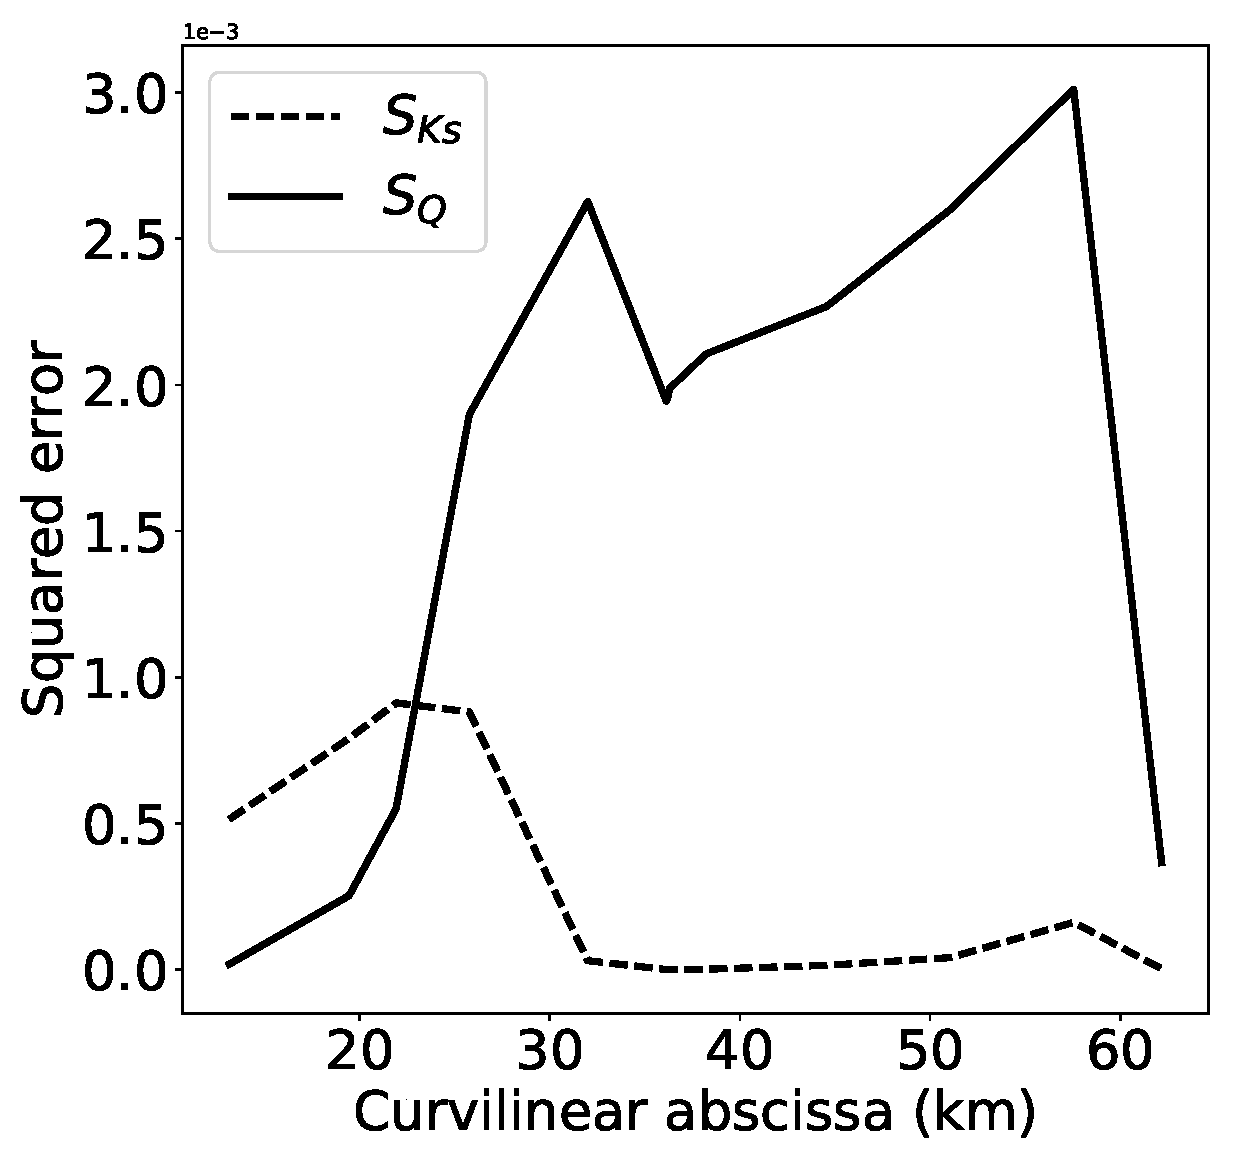
\includegraphics[width=0.47\linewidth,height=\textheight,keepaspectratio]{fig/applications/mascaret/Fig6a.pdf}}
\subfloat[PC -- 121 snapshots]{
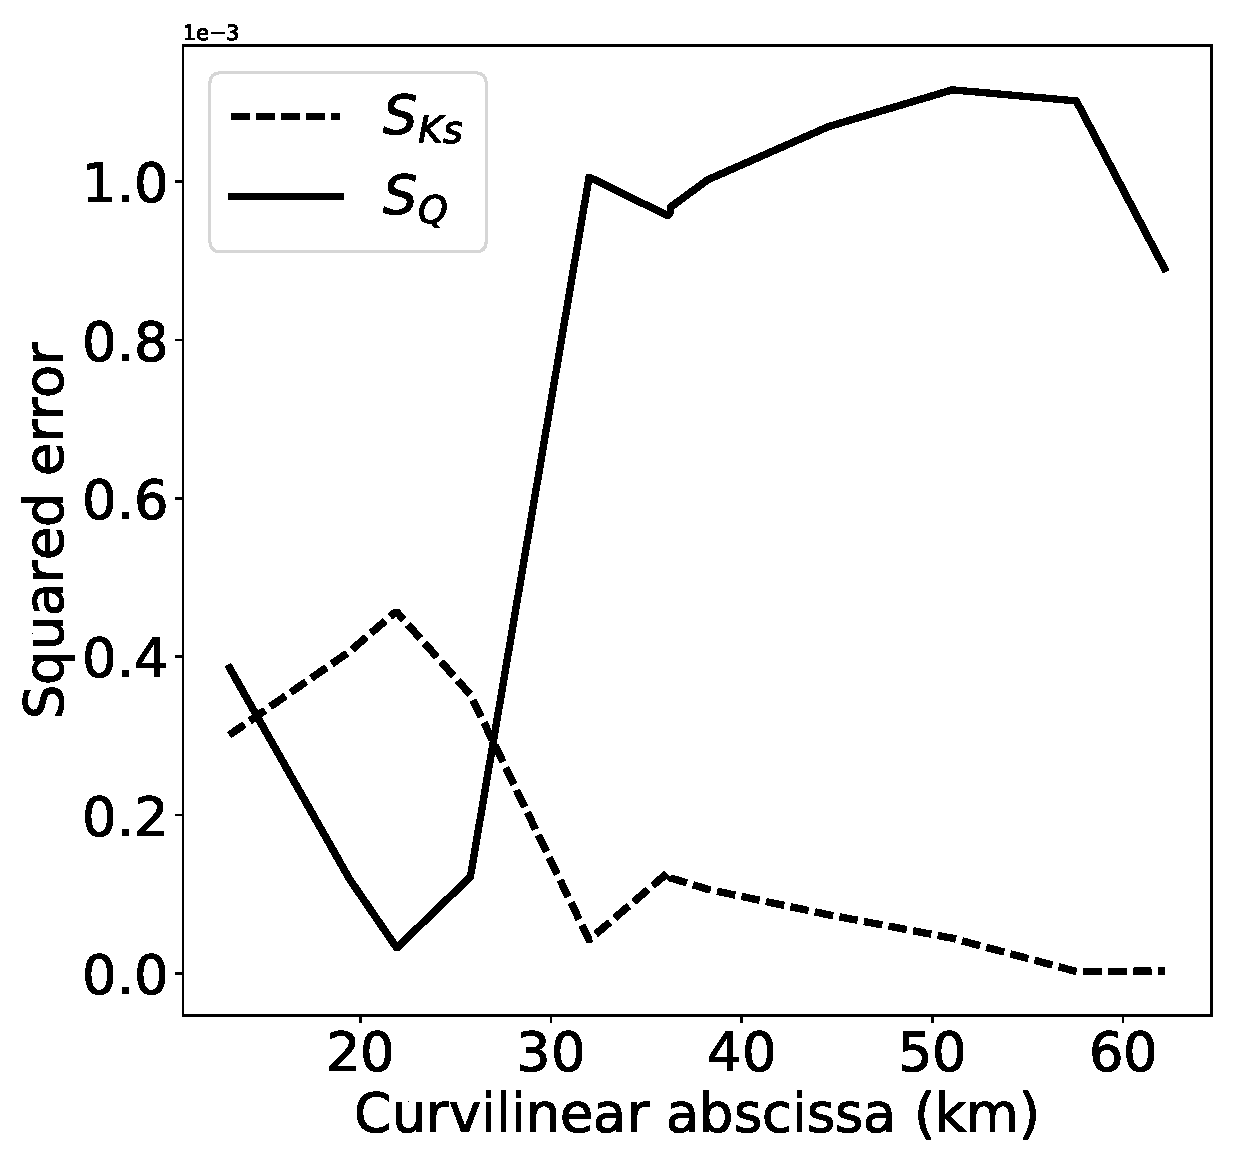
\includegraphics[width=0.47\linewidth,height=\textheight,keepaspectratio]{fig/applications/mascaret/Fig6b.pdf}}
\caption{Squared error of the spatial Sobol' indices along the 50 km reach for (a)~pGP and (b)~PC surrogate models built using $N = 121$ snapshots in the training set. Dashed lines correspond to the Sobol' index associated with $K_{s_3}$; solid lines correspond to that associated with the upstream discharge $Q$.}
\label{fig:sobol-map}
\end{figure*}

\begin{figure*}[!h]               
\centering
\subfloat[pGP -- 121 snapshots]{
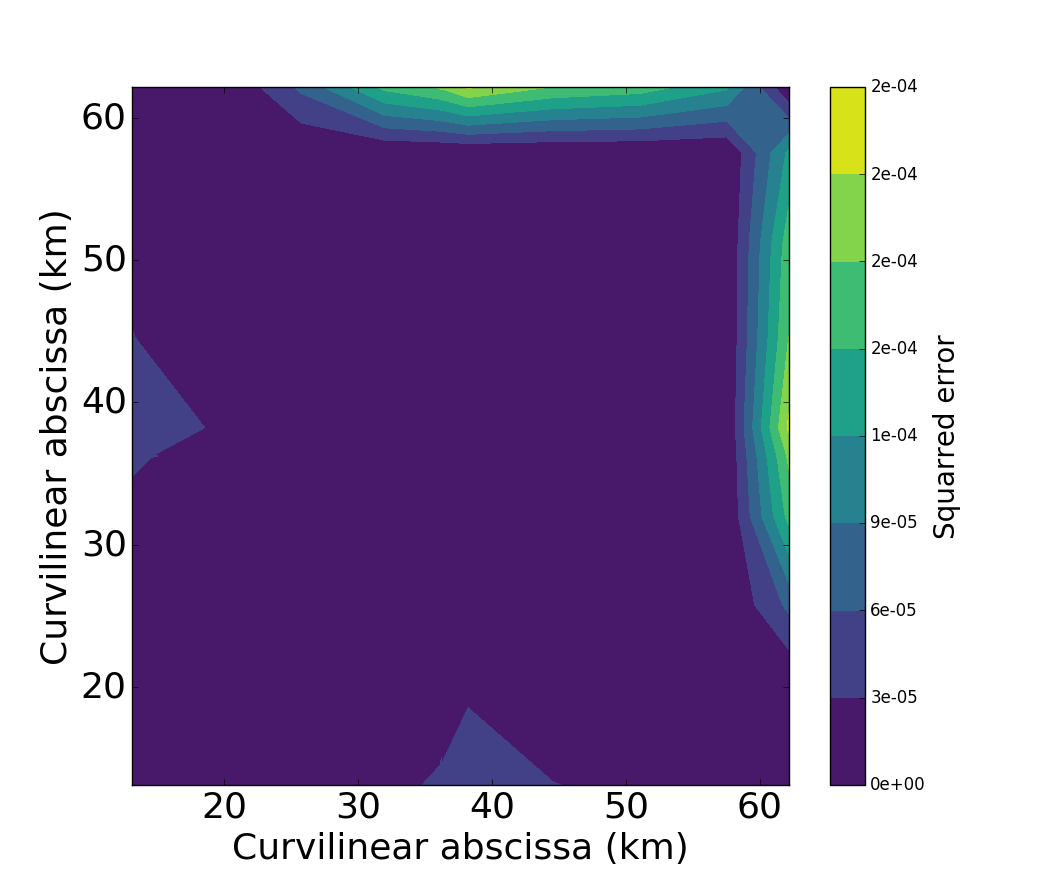
\includegraphics[width=0.47\linewidth,height=\textheight,keepaspectratio]{fig/applications/mascaret/Fig7a.png}}
 ~ 
\subfloat[PC -- 121 snapshots]{
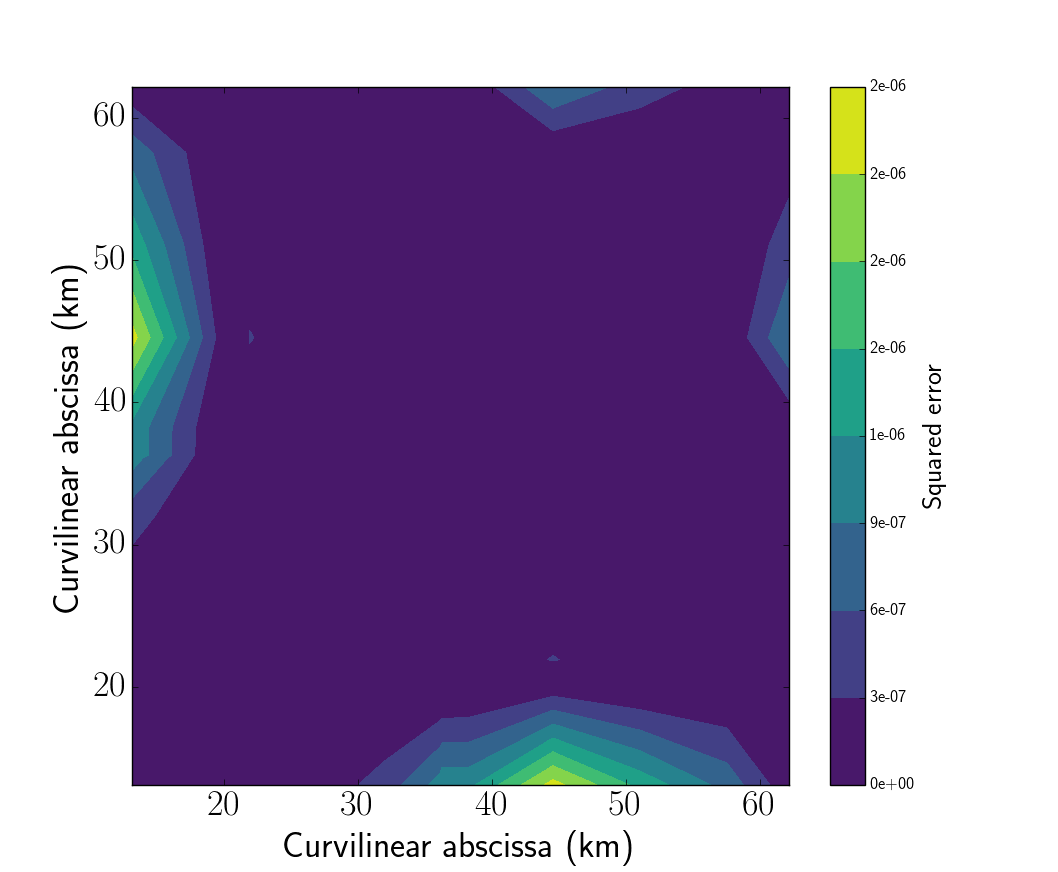
\includegraphics[width=0.47\linewidth,height=\textheight,keepaspectratio]{fig/applications/mascaret/Fig7b.png}}
\caption{Squared error of the correlation matrix for (a)~pGP and (b)~PC surrogate models built using $N = 121$ snapshots.}
\label{fig:corr-mse}
\end{figure*}

\section{Conclusion}\label{sec:ccl}

The purpose of this work was to compare two popular strategies for building surrogate models, Polynomial Chaos (PC) and POD-based Gaussian Process (pGP). Both methods were applied to a hydraulic case corresponding to a spatially distributed open-channel steady flow along the Garonne River depending on the upstream discharge $Q$ and on the Strickler friction coefficient $K_{s_3}$, with the long-term objective to determine which surrogate strategy could be useful in the framework of ensemble-based data assimilation. It is important to show how surrogate models could be used to estimate some statistical quantities in a cost-effective way. This is useful for sensitivity analysis studies to evaluate the impact of physical parameters and external forcing on the river state. This is also useful for data assimilation to estimate correlation matrix and PDF related to the spatially distributed river state for the Ensemble Kalman Filter (EnKF) and the Particle Filter (PF), respectively.

We carried out a convergence study based on the following metrics: water level statistical moments, correlation matrix, PDF as well as Sobol' indices representing the contribution of the upstream discharge and the Strickler friction coefficient on the water level variance. The accuracy of the PC and pGP surrogates were measured by their ability to retrieve the reference metrics obtained with a converged Monte Carlo (MC) random sample (including $\numprint{100,000}$ MASCARET simulations). An in-depth comparison of these metrics was done using the same computational budget: 121 MASCARET snapshots. The sensitivity to the number of snapshots was carried out to ensure that 121 simulations were enough to make this comparison valuable.

Results showed that both surrogate models can be used in place of the MASCARET forward model for uncertainty propagation without loss of accuracy. None of the two surrogate models clearly outperforms the other. In both cases, the PC and pGP surrogate models are able to correctly retrieve all physical information. The PC strategy seems to be more precise to compute the spatially distributed correlations as well as the Sobol' indices, with the advantage that these indices do not need any further MASCARET evaluation as they are analytically computed from the PC expansion. Still, the multimodal water level PDF at Marmande (which is an important observation station along the Garonne River in operational context) was better captured by the pGP strategy that requires an additional sampling of the surrogate. Indeed, even increasing the number of snapshots to 256 and beyond was not enough to retrieve the second mode of the PDF using the PC surrogate model, while this was already captured with 121 snapshots by the pGP surrogate model. Still, it should be mentioned that the PC model better positions the first mode than the pGP model when using the MC approach as reference. Last but not least, the PC strategy requires some insight about the uncertain inputs of the system. We may not have access to this information in practice, leading potentially to a poor robustness of the PC surrogate. The quantity of interest may also feature non-linearity and exhibit extrema, which could be difficult to account for using quadrature points that could miss some physics. Alternative (for instance sparse) projection strategies could be investigated in the future to overcome these limitations. 

Conclusions for the present test case highlight the validity of both quadrature-based PC and POD-based GP surrogate strategies for SWE in permanent flow for a small dimensional problem (the size of the uncertain space is $d = 2$). The ranking between PC and pGP approaches will need to be further investigated when moving to open-channel unsteady flow modelling used for instance in the context of operational flood forecasting. The first challenge lies in the extension of the PC and pGP surrogates to larger uncertain dimension $d$, especially to address parameters that vary in space or over time or both, such as the bathymetry spatial field and the time series of the upstream discharge. This may require the evaluation of more advanced strategies to reduce the size of the basis, the uncertain dimension (for instance through the Karhunen-Loève transformation) and the number of snapshots $N$ in the training set. For instance, the quadrature method used to build the PC surrogate is known to suffer from the \emph{curse-of-dimensionality}. This will have to be revisited for a larger size $d$ of the uncertain space. The second challenge lies in the validity of the surrogate model over successive data assimilation cycles, implying that the flow is now unsteady. First, it is expected that the SA shows that the roughness coefficients from upstream and downstream locations have an influence on the flow at a given location in subcritical flow. Secondly, it may be necessary to adjust the coefficients of the surrogates to track the changes in the river state behaviour over time. The cycled data assimilation analysis will then allow to correct physical parameters over time, such as the roughness coefficient that may vary seasonally or between flood events. The uncertainty quantification and data assimilation strategies could also be extended to the bathymetry and thus allow for a time-varying correction of the river geometry that is usually fixed in a hydraulic model. Such solution would mimic the evolution of the river bed and flood plain at a much lower computational cost than when using a hydro-sediment coupled model.

Those are crucial steps for the complementary use of surrogate models within data assimilation algorithms.


\chapter{LS89}\label{chap:ls89}

\section{Introduction}

The number of CFD simulations that is required for the formulation of the surrogate model is defined by the complexity of the physics and the number of input parameters to take into account. This factor is paramount when considering costly numerical simulations. As the accuracy of an uncertainty quantification being directly correlated to the quality of the surrogate~\cite{iooss2010}, the present study aims at improving its construction by using the two new strategies for resampling the parameter space (see~\cref{chap:resample}). An industrial application is targeted: the aerothermal analysis around the \textit{LS89} vane~\cite{arts1990}. An Uncertainty Quantification study has already been performed using Reynolds Averaged Navier-Stokes (RANS)~\cite{Gourdain2010,emory2016} but the first UQ analysis using Large Eddy Simulation (LES) is here presented. LES are high-fidelity full 3D unsteady simulations. This approach comes at a high CPU cost which requires the use of High Performance Computing (HPC) resources.

The chapter is tailored as follows; \cref{sec:ls89_case} presents the experimental setup while \cref{sec:ls89_num} presents its numerical simulation configuration. Finally, \cref{sec:ls89_results}  presents the results of the UQ.

\section{Case description}\label{sec:ls89_case}
The \textit{LS89} case is a blade cascade designed and tested experimentally at the Von Karman Institute for Fluid Dynamics (VKI)~\cite{arts1990}. The linear cascade consists of five high-pressure turbine vanes although only the centre vane is studied---see~\cref{fig:vki-setup}. The vane is a 2D extruded profile unlike most industrial vanes that are much more complex geometrically. It, however, remains of great interest because the operating points are representative of values found in real engines today. This test case represents one of the largest turbomachinery databases available for the validation of CFD models in complex geometries.

\begin{figure}[!h]               
\centering
\subfloat[VKI installation]{
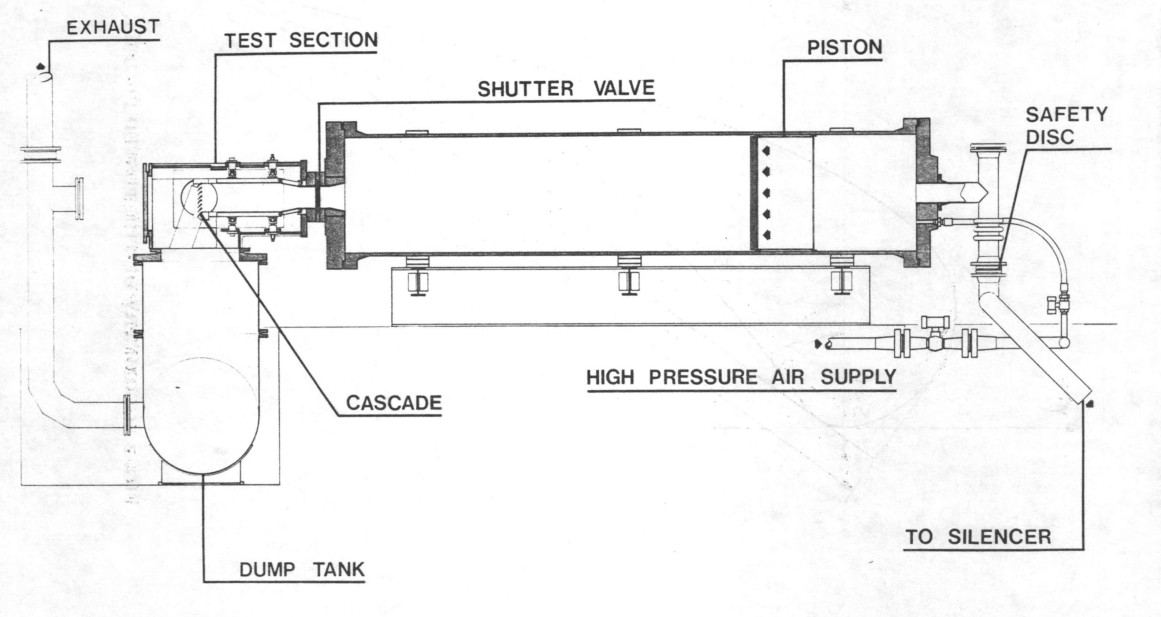
\includegraphics[width=0.7\linewidth,height=\textheight,keepaspectratio]{fig/applications/ls89/VKI.png}}
 ~       
\subfloat[Blade profile]{
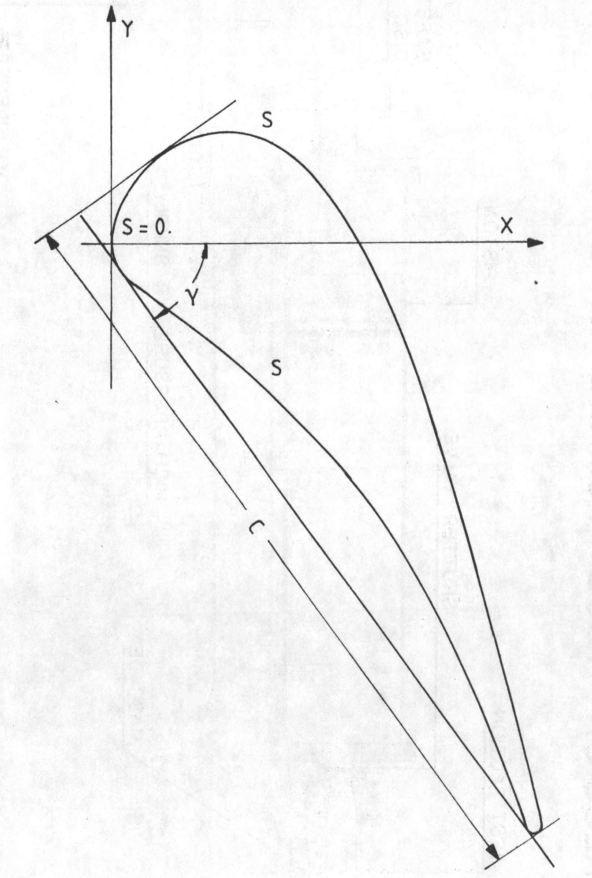
\includegraphics[width=0.3\linewidth,height=\textheight,keepaspectratio]{fig/applications/ls89/blade.png}}
\qquad       
\subfloat[Geometrical Characteristics]{

%\begin{table}[H]
%\centering
\begin{tabular}[b]{lc}
\toprule
 $c$ (mm) &  67,647 \\
 $g/c$& 0,850\\
 $\gamma$ (degr.)& 55,0\\
 $o/c$& 0,2207 \\
 $r_{LE}/c$& 0,061\\
 $r_{TE}/c$& 0,0105\\
\bottomrule
\end{tabular}
%% \label{}
%\end{table}

}
\caption{LS89 blade cascade experimental setup from the VKI. Source~\cite{arts1990}}
\label{fig:vki-setup}
\end{figure}

A large variety of operating points have been successfully simulated until now. Low levels of turbulence injection ($<1$\%) do not represent an issue for most solvers \cite{Gourdain2010,emory2016} using either Reynolds-Averaged Navier Stokes (RANS) or Large Eddy Simulation (LES). Higher levels of turbulence have also been studied successfully~\cite{Wheeler2015} but difficulties arise for higher Reynolds numbers and larger outlet Mach numbers. Simulations are not able to correctly predict experimentally obtained profiles, notably the heat transfer field which is of great importance for the blade life-cycle.

The operating point addressed in this document, selected from Arts~\cite{arts1990}, is the MUR235, a very rich case in terms of physics that presents the above mentioned challenges (high Reynolds and outlet Mach numbers)---see~\cref{tab:ls89-param} and \cref{tab:ls89-limite}. Figure~\ref{fig:ls89-gradRhoRho} highlights the main physical interactions in such a flow. One of the most notable features is the presence of a shock wave on the suction side of the blade. This shock wave interacts with a transitional boundary layer due to the highly curved flow, a potential source of instabilities in the boundary layer which in turn determines the wake downstream. This wake issues acoustic waves that impact the neighbour blade affecting the stability of the boundary layer. Also, there is a high level of free-stream turbulence that undergoes stretching around the leading edge of the blade which modifies the position of the boundary layer transition on the suction side~\cite{Segui2017a}.


\begin{table}[!h]
\centering
\begin{tabular}{lc}
\toprule
Total temperature (K)&413,30 \\
Total inlet pressure (bar)&1,828 \\
Static inlet pressure (bar)&1,800 \\
Static outlet pressure (bar)&1,049 \\
Wall temperature (K)&301,15 \\
Free stream turbulence (\%)&6,0 \\
Incidence angle (degr.)&0,0 \\
\bottomrule
\end{tabular}
\caption{Measured parameters for the MUR235 case.}
\label{tab:ls89-param}
\end{table}

\begin{table}[!h]
\centering
\begin{tabular}{lcc}
\toprule
 & Inlet & Outlet \\
\midrule % \cmidrule{2-3}
Total temperature (K)&413,3& \\
Total pressure (bar)&1,828& \\
Mach number&0,150&0,927 \\
Reynolds number&\numprint{2,6471e5}& \numprint{1.1521e6} \\
Temperature (K)&411,45& 352,69\\
Pressure (bar)&1,800& 1,049\\
Density (\unit{}{\kilogram\per\cubic\meter})&1,524& 1,036 \\
Velocity(\unit{}{\meter\per\second})&61,00& 349,02 \\
Dynamic viscosity (\unit{}{\kilogram\per\meter\second})& \numprint{2,33750e-5}& \numprint{2,1240e-5}\\
Kinematic viscosity(\unit{}{\meter^2\per\second})&\numprint{1,5589e-5}& \numprint{2,0494e-5}\\
\bottomrule
\end{tabular}
\caption{Free stream conditions for the MUR235 case.}
\label{tab:ls89-limite}
\end{table}



%Until now, simulations have shown disparate results and capacities to predict the heat transfer coefficient, $H = \frac{\dot{q}_{wall}}{T_0 - T_{wall}}$, where ${\dot{q}_{wall}}$ is the heat flux, $T_0$ is the total inlet temperature and $T_{wall}$ is the temperature on the blade surface.

\begin{figure*}[!h]
\centering
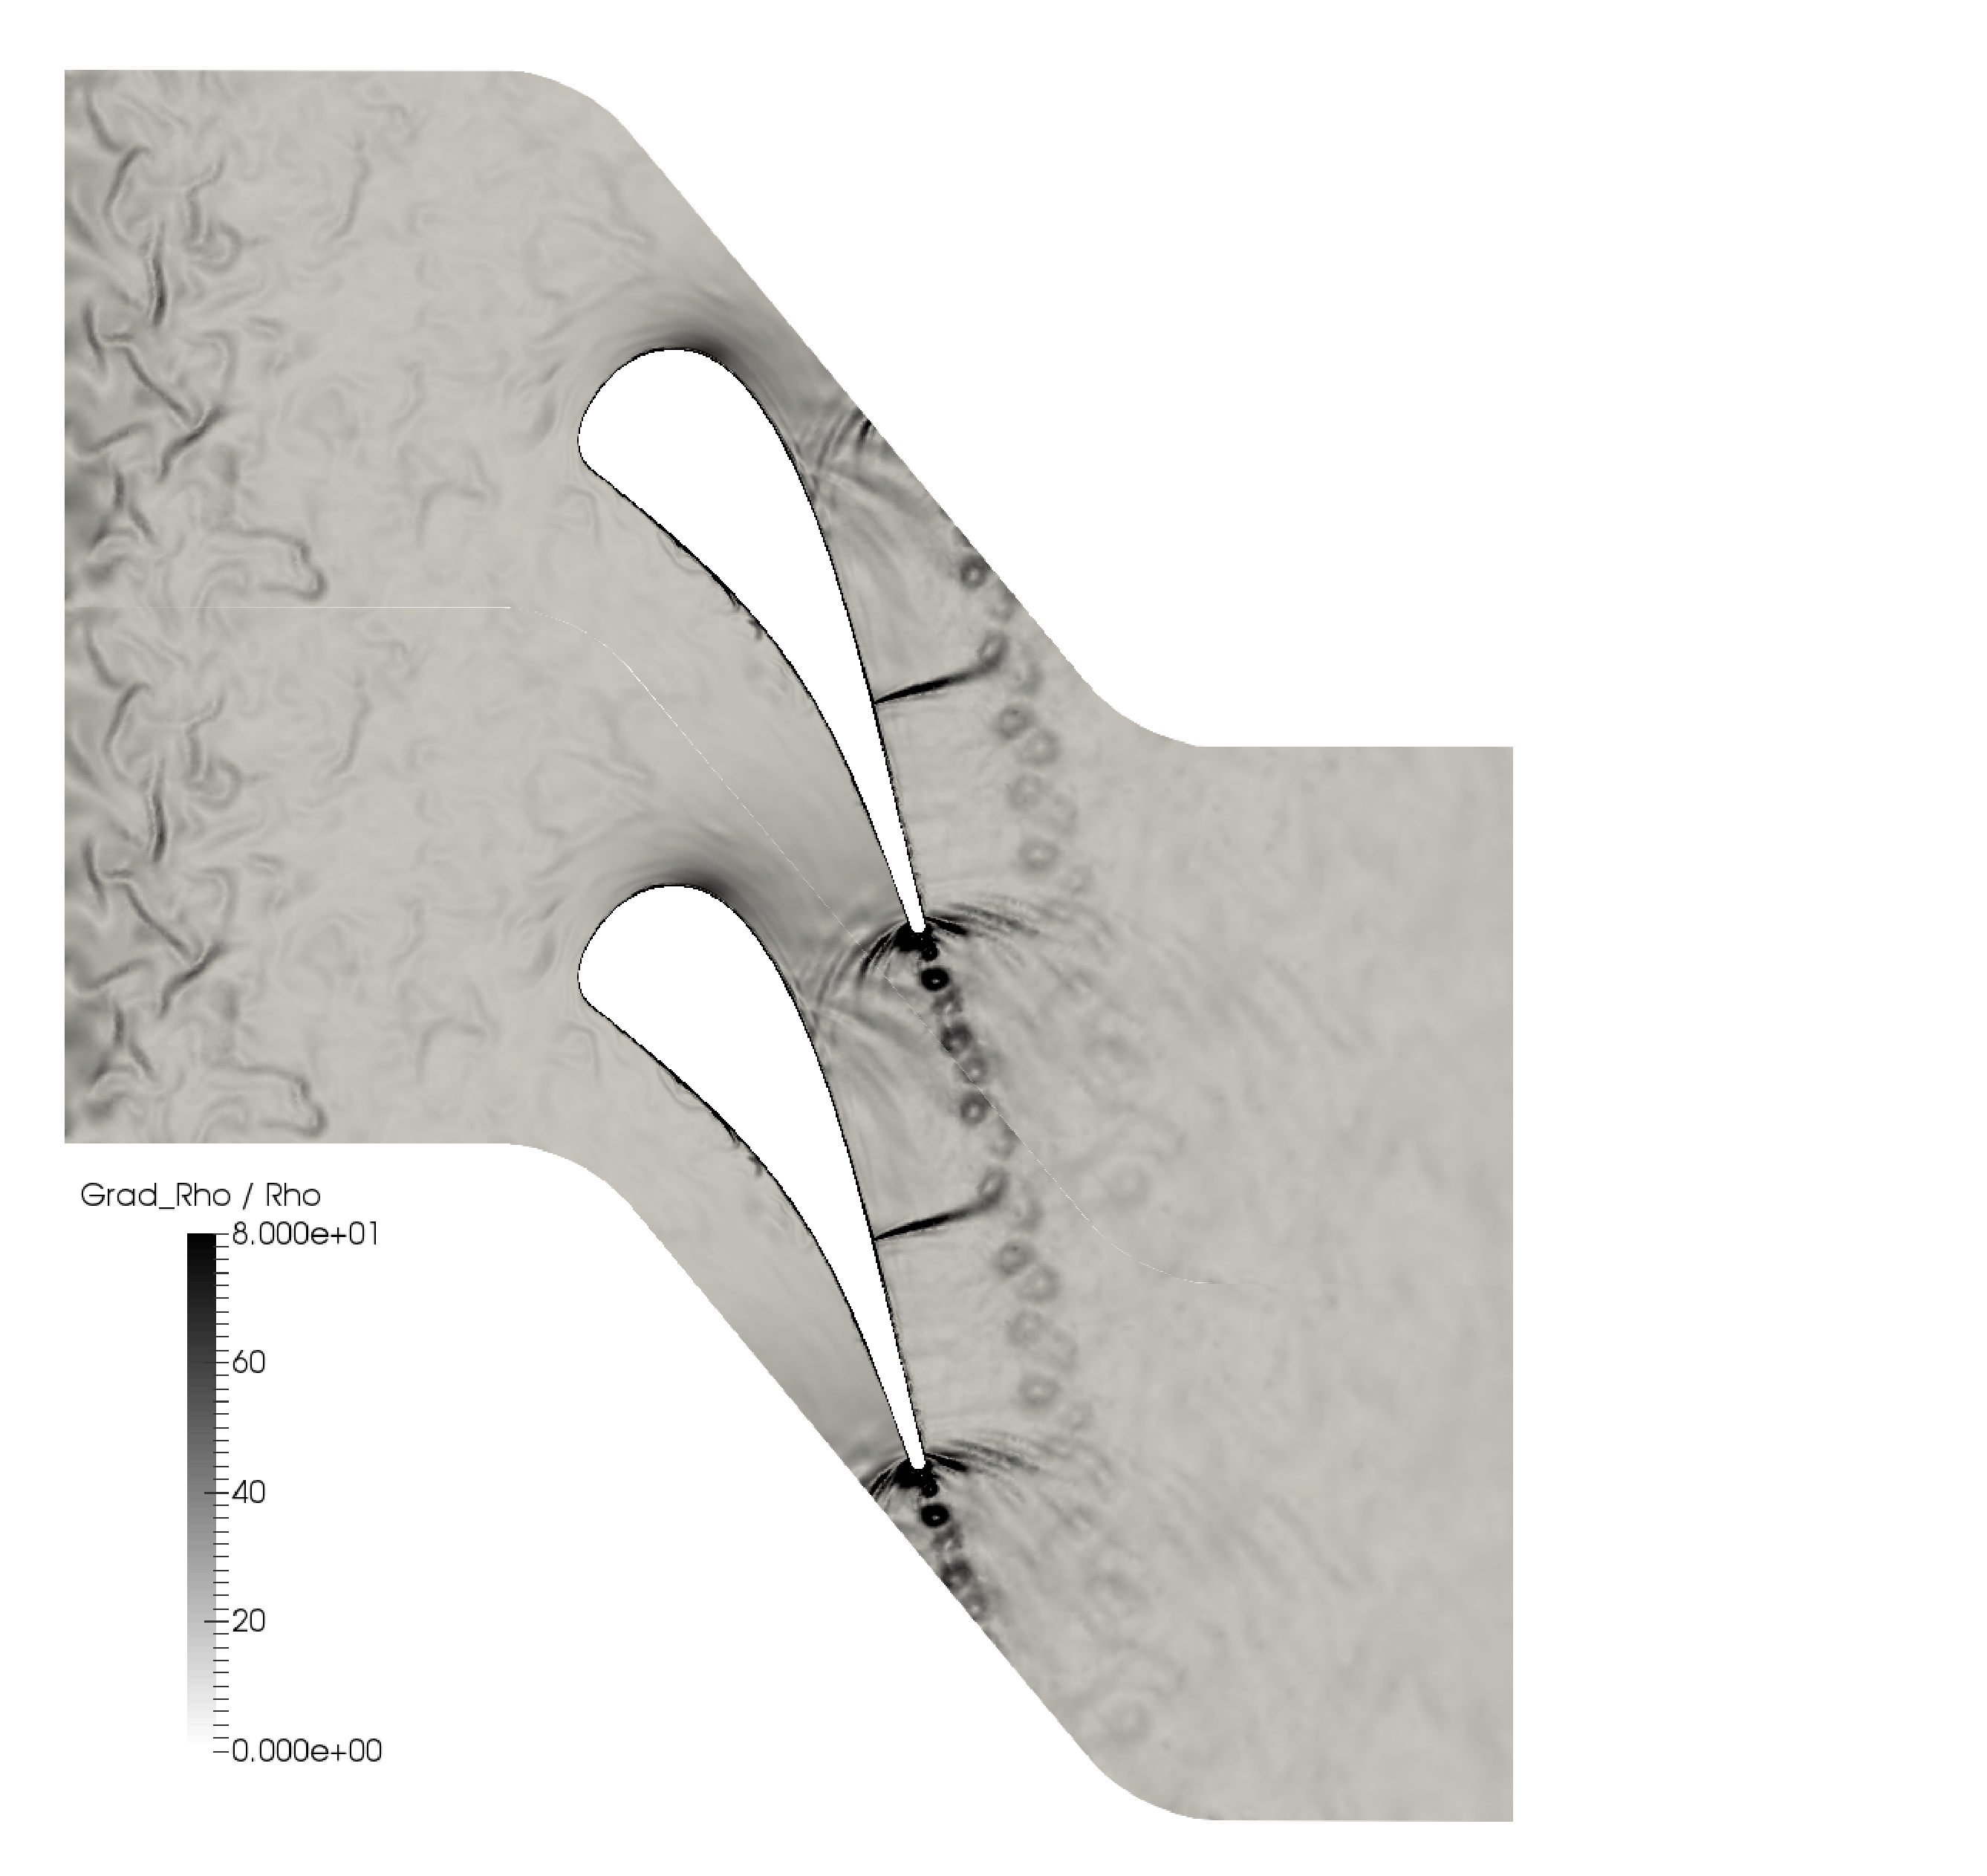
\includegraphics[width=0.6\linewidth,keepaspectratio]{fig/applications/ls89/10_2column_color-online-only_gradRhoRho.pdf}
\caption{$\frac{\nabla \rho}{\rho}\; (m^{-1})$ with $Tu = 30\%$.}
\label{fig:ls89-gradRhoRho}
\end{figure*}

%It is precisely the transition on the suction side which is targeted. This operating point has the particular difficulty of capturing the heat flux on the suction side in the region between approximately 25~mm, where the acoustic waves impact the surface blade, and 62~mm the approximate shock position. 

In the original experiments~\cite{arts1990}, an increase in heat transfer is observed on the suction side of the blade when a high turbulence intensity level at the inlet ($\sim 6$\%) as well as a large Reynolds number at the outlet ($>\numprint{1e6}$) are present. The simulations recover the shock wave that triggers an abrupt transition of the boundary layer, but turbulent spots may be found upstream of this position that can contribute to the overall heat transfer. These spots can be explained due to perturbations in the free-stream turbulence $Tu$ that are capable of trespassing the sheltering effect of the shear layer and thereby increase the heat transfer. Turbulence values upstream of the blade are thus of upmost importance.

The original experiments give only the turbulence intensity level at an upstream distance from the vane, which is insufficient to characterize the turbulent flow at this location. Recent studies on the same test bench have measured the integral length scale for the same intensity level~\cite{Fontaneto2014}. In spite of this newly available information, simulations are not capable of recovering an important part of the heat flux on the suction side even when taking the correct length scale~\cite{Pichler2016}. Uncertainties concerning the measured values in the experiments, that serve as boundary conditions in the simulation, appear as a path to be explored. 

Apart from the turbulence intensity and the length scale, the angle of attack $\alpha$ of the incoming flow can also be seen as an uncertain parameter. There is no information related to this parameter in the experimental campaigns. In~\cref{fig:space-tu-alpha}, the effect of $\alpha$ was numerically investigated with respect to $Tu$ by studying the heat transfer coefficient response---hereafter defined as the QoI. Due to the computational effort required to modify and simulate a case correctly with a modified integral length scale versus a modification of $\alpha$, this parameter was not taken into account. Increasing $Tu$ or $\alpha$ causes an increase of the QoI and $Tu$ seems to have a larger impact than $\alpha$. A deeper analysis would require more computations to obtain: \textit{(i)} a correct response of the influence of these parameters on the QoI ; \textit{(ii)} the contribution of each parameter ; and \textit{(iii)} the probability density function of the QoI by propagating the uncertainties. Thus, the parameter space for this study was defined as
\begin{align}
Tu \in [0, 30\%] \quad \alpha \in [-5,5\degree].
\end{align}

\begin{figure*}[!h]
\centering
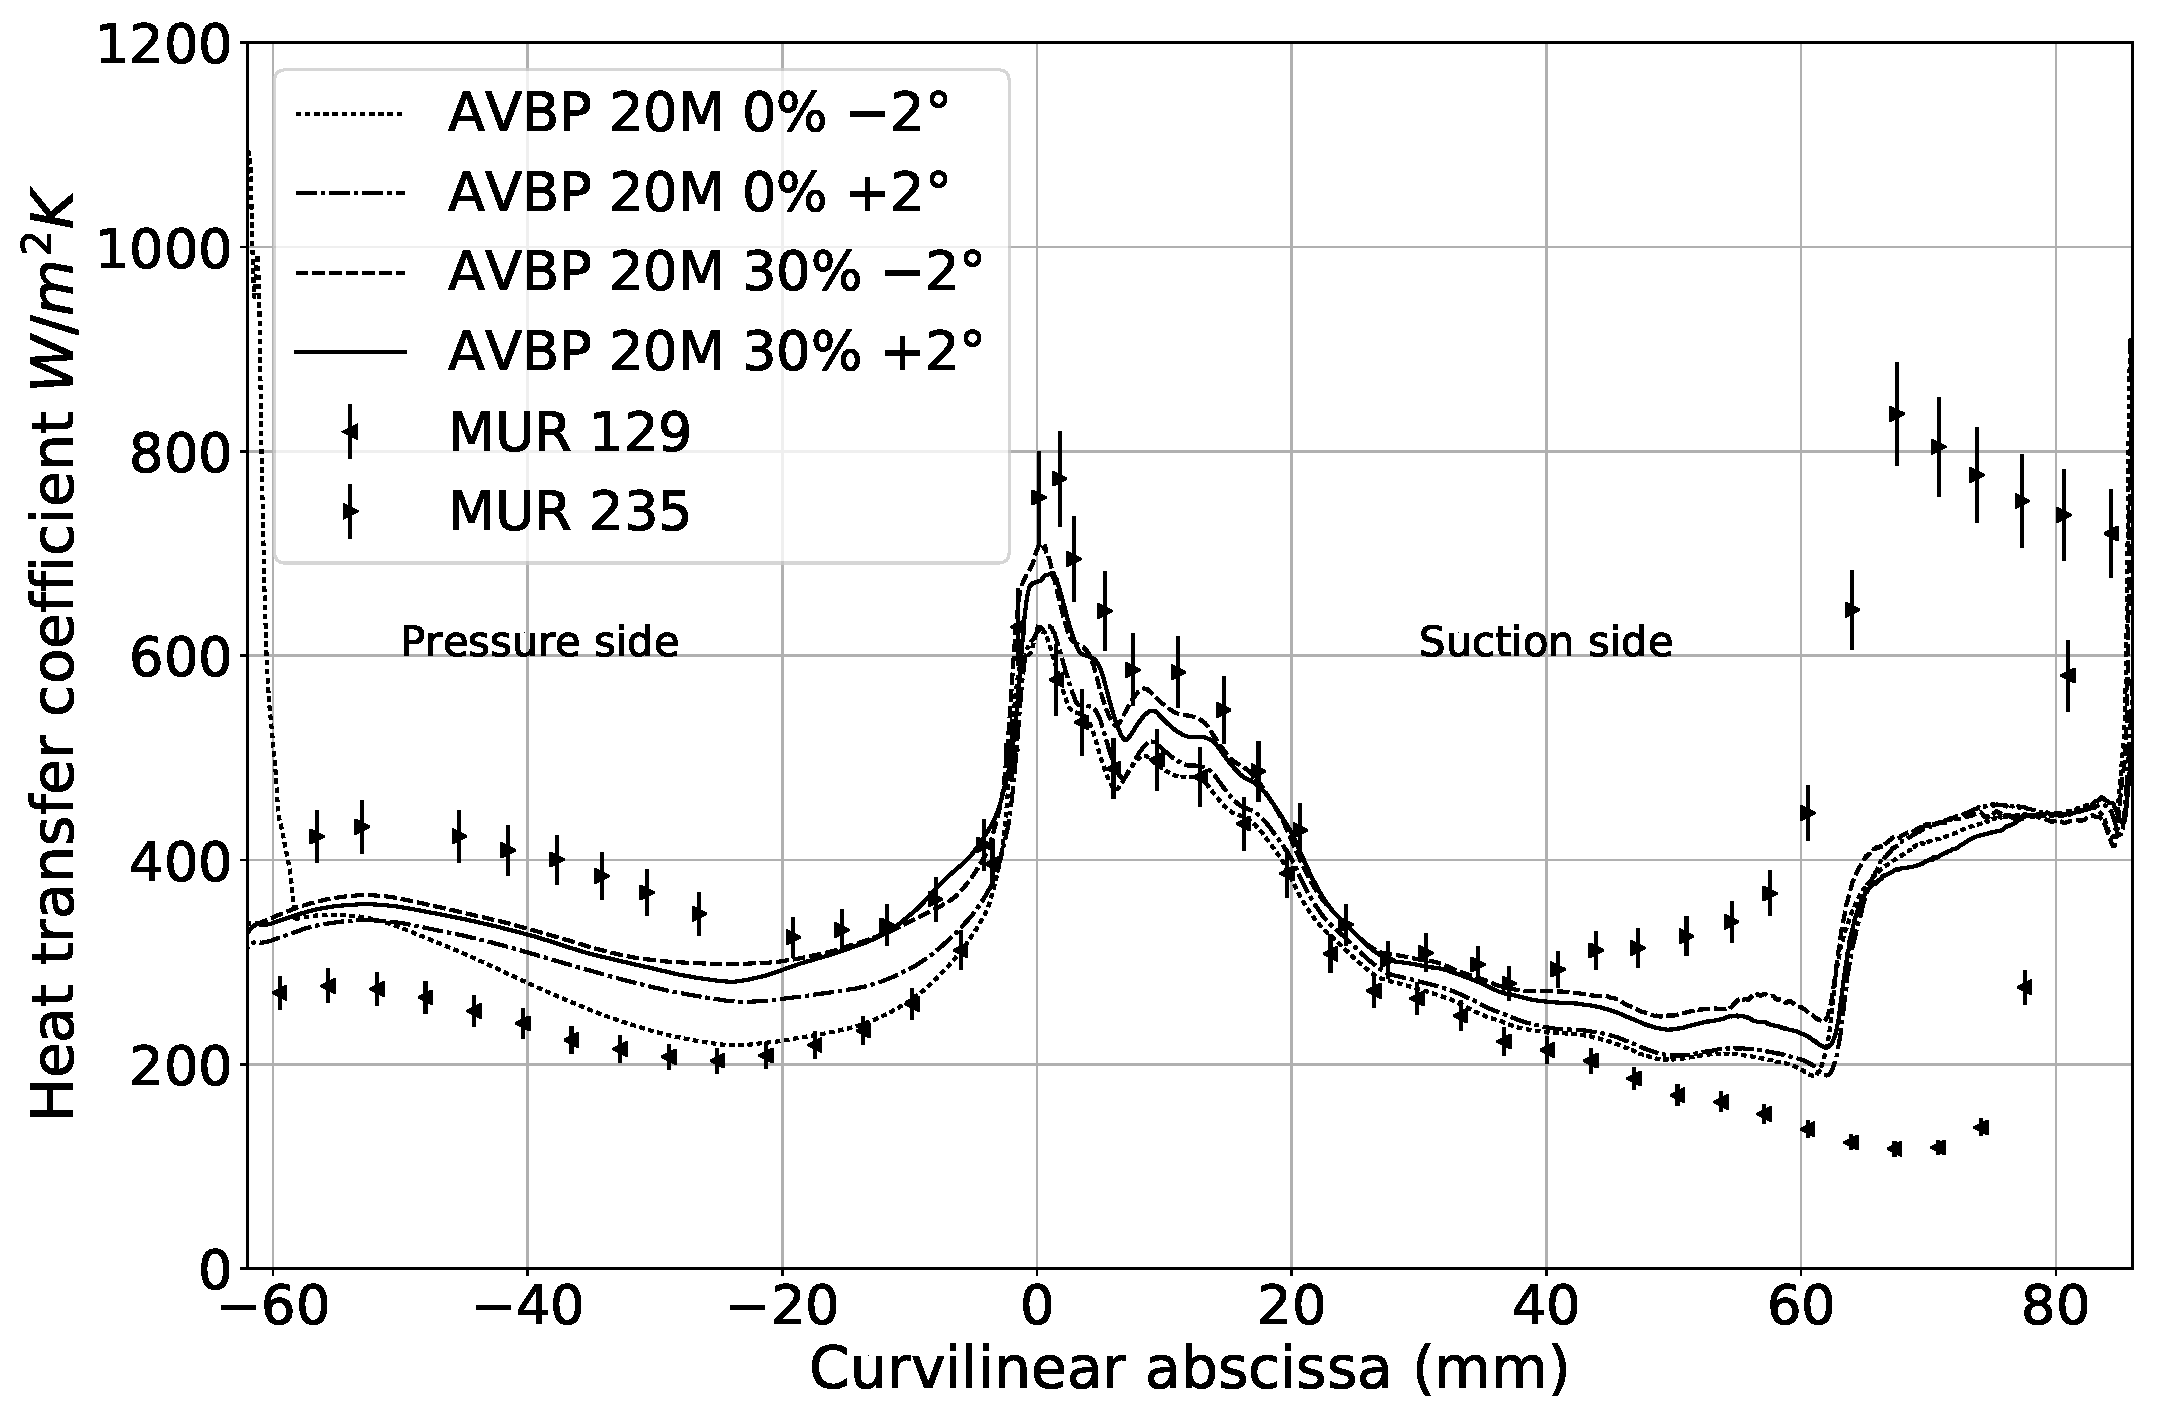
\includegraphics[width=0.9\linewidth,keepaspectratio]{fig/applications/ls89/11_2column_color-online-only_space_tu-alpha.pdf}
\caption{Heat transfer coefficient variation compared to experimental data of MUR129 ($Tu=1\%, \alpha = 0\degree$) and MUR235 ($Tu=6\%, \alpha = 0\degree$).}
\label{fig:space-tu-alpha}
\end{figure*}

\section{Numerical setup}\label{sec:ls89_num}

The simulations have been performed using \textit{AVBP}~\cite{Gicquel2011}, a validated CFD LES solver co-developed by CERFACS and IFP-EN. This parallel code solves the three-dimensional compressible Navier-Stokes equations for both steady and unsteady reacting flows. The code is capable of handling hybrid unstructured meshes and allows to address complex geometries. High-order numerical schemes based on the \textit{Taylor-Galerkin} (TTG) family are used~\cite{Quartapelle1993}. 

The simulations were performed on a 20 million cells mesh. Five layers of prisms in the near-wall region are present allowing a higher aspect ratio. The mean $\overline{y^+}$ has a value of $\simeq 6.62$ which limits the physical time step to $\unit{\numprint{1.94e-8}}{\second}$. In this context, a wall-resolved computation using the \textit{WALE} \cite{Nicoud1999} model is used to take into account the proper turbulence scaling in the near-wall region. To gather enough statistics, a simulation time of $\unit{\sim\numprint{4.1}}{\milli\second}$ was performed. This led to a CPU cost, for a single computation, of $\sim7500$~hours lasting $\sim5$~hours on a cluster of 1440 cores.

The resolution of the mesh and the LES quality must be guaranteed to be sufficient to capture the complex physics encountered. Indeed, the interaction between the free-stream turbulence and the boundary layer requires to carefully mesh the near-wall region. It is reasonable then to compare the profiles of heat transfer obtained using the mesh for this UQ study, from here on denoted as \textit{M0}, to two finer meshes \text{M1} and \textit{M2}, see ~\cref{fig:M0M1M2_hcomp}. The corresponding spatial distributions of ${y^+}$ are shown in~\cref{fig:M0M1M2_y+comp} for the three meshes.

\begin{figure*}[!h]
\centering
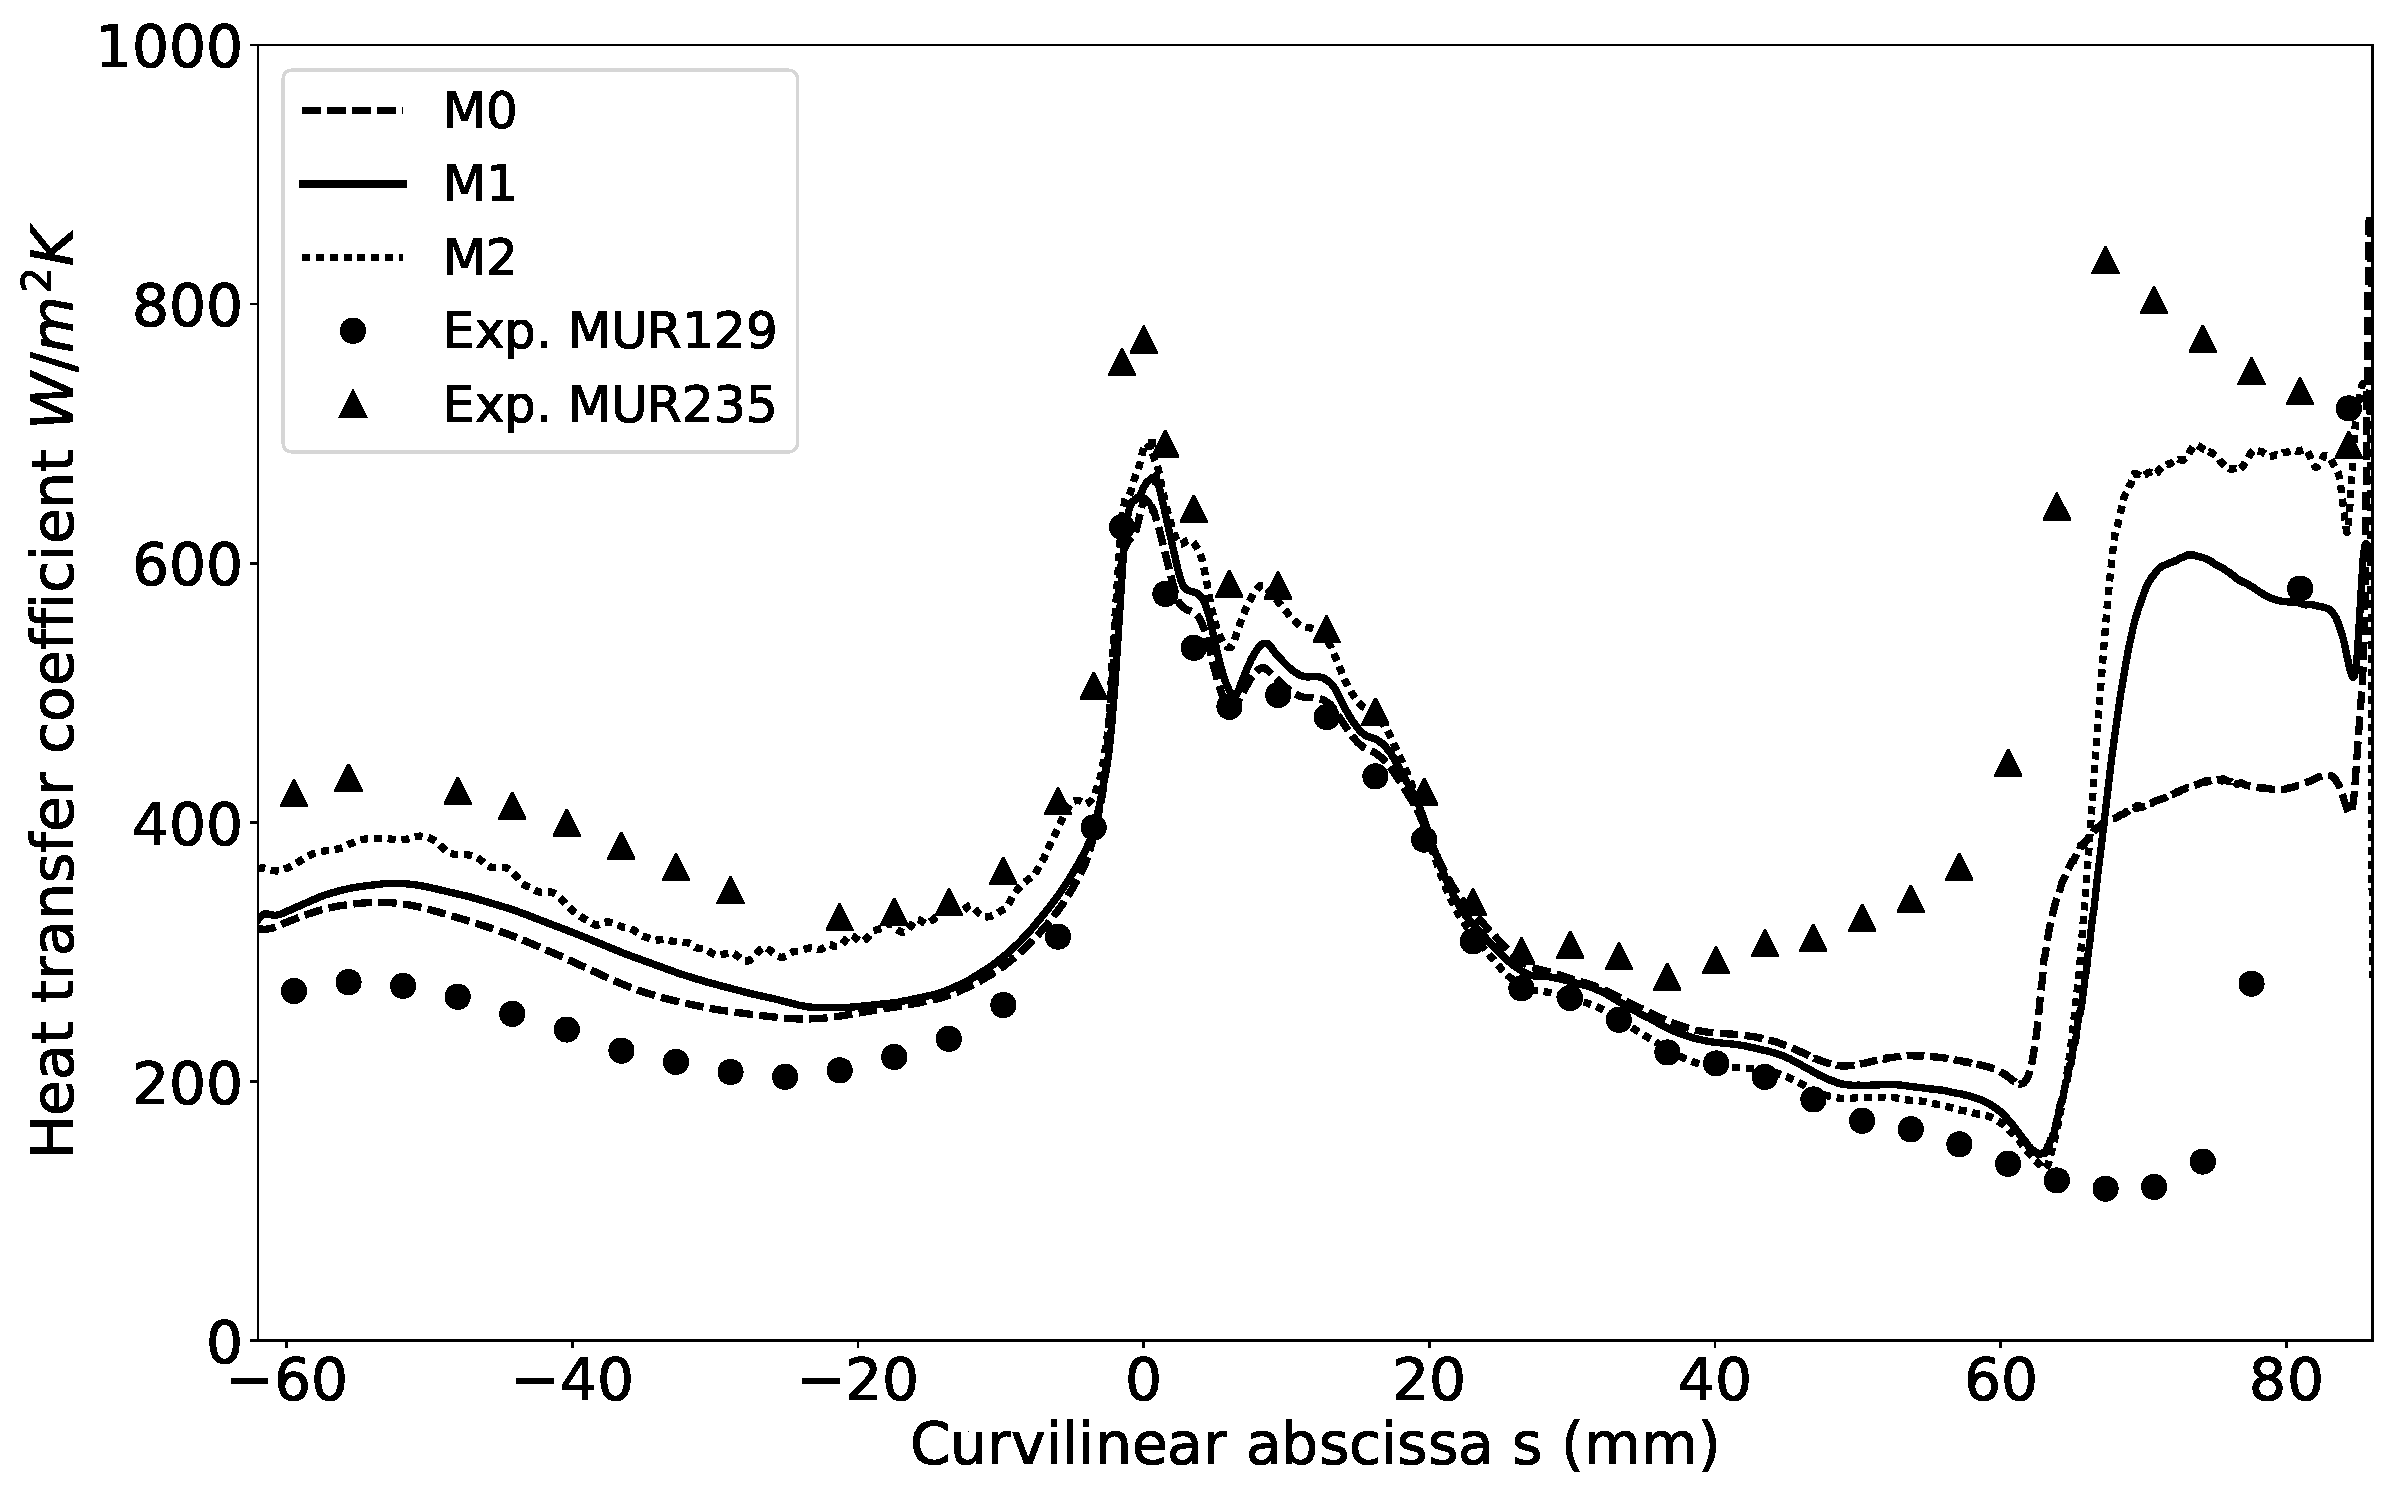
\includegraphics[width=0.8\linewidth,keepaspectratio]{fig/applications/ls89/Heatflux_M0M1M2_comp.pdf}
\caption{Heat transfer coefficient between various meshes using MUR235 setup ($Tu=6\%, \alpha = 0\degree$).}
\label{fig:M0M1M2_hcomp}
\end{figure*}

\begin{figure*}[!h]
\centering
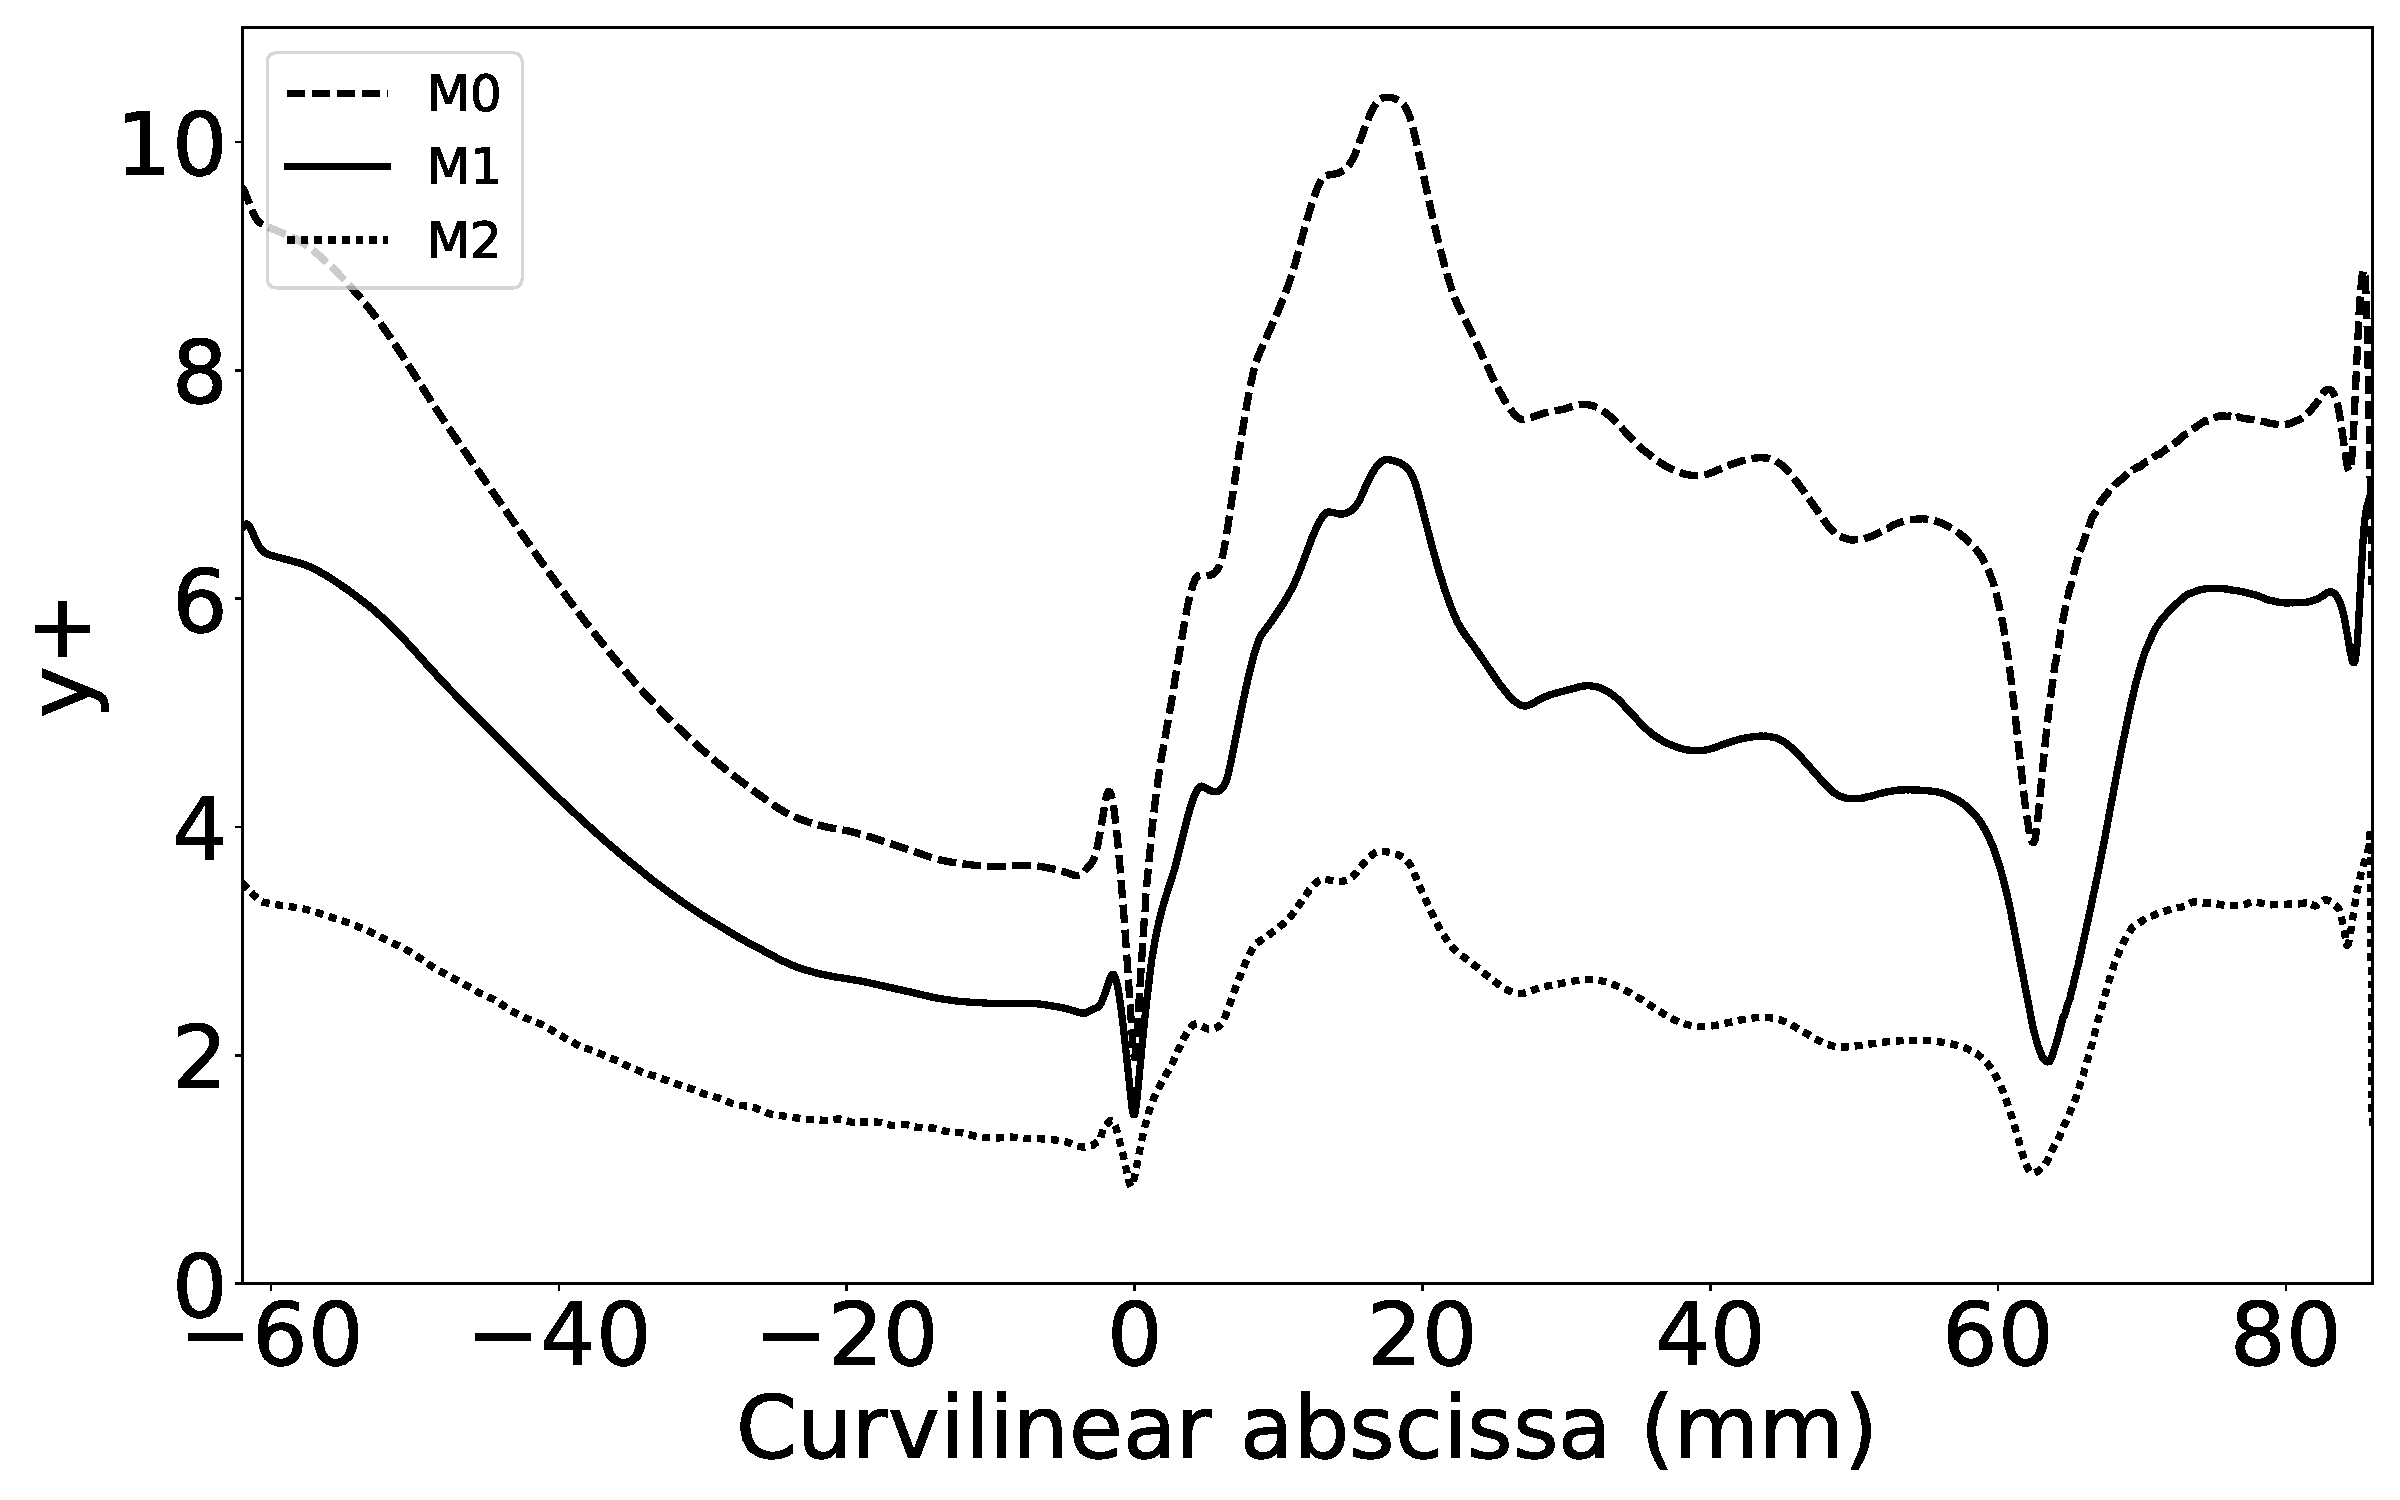
\includegraphics[width=0.8\linewidth,keepaspectratio]{fig/applications/ls89/yplus_M0M1M2_comp.pdf}
\caption{Refinement over blade surface measured using non-dimensional $y^+$ parameter for MUR235 operating point ($Tu=6\%, \alpha = 0\degree$).}
\label{fig:M0M1M2_y+comp}
\end{figure*}

The heat transfer coefficient is seen to be different on the pressure side for the finest mesh (M2). However, on the suction side the coarsest mesh (M0) leads to approximately the same results as the finest mesh (M2). This suggests that the value of $y^+$ does not have a first order effect on the heat transfer coefficient for the meshes considered. The sensitivity to other effects such as turbulence intensity and angle of attack may thus be sought. Additionally, it can be noted that the shock wave on the suction side is located at approximately the same position for all meshes. This implies that the upstream boundary layer is similar in all cases although the heat transfer coefficient across the shock wave is affected by the mesh refinement.

\section{Uncertainty Quantification results}\label{sec:ls89_results}

This section presents the comparison between the different resampling methods on this complex case. In the following, an existing sample comprised of 16 simulations is used to generate a \textit{Sobol'} low-discrepancy sequence. As seen in~\cref{sec:doe}, the quality of \textit{Sobol'} sequence is similar to \textit{Halton}'s in low dimensional cases. Using this initial set of simulations, the sequence has been continued adding 4 points to give a total of 20 simulations. Then using the same initial sample, the previous set is compared to the use of the $\sigma$ method and the LOO-\textit{Sobol'} method. The LOO-$\sigma$ method gives similar results compared to LOO-\textit{Sobol'} method. It is not tested on this case. Quality results evaluated by LOO as described in~\cref{sec:error} are shown in~\cref{tab:ls89-q2}. 

\begin{table}[h]
\centering
\begin{tabular}{lcc}
\toprule
Method & Number of Simulations &$\hat{Q}_2$\\
\cmidrule{2-3}
\textit{Sobol'}&16 & 0.638\\
\textit{Sobol'}&20& 0.821\\
\textit{$\sigma$}&20& 0.688\\
LOO-\textit{Sobol'}&20& 0.856\\
\bottomrule
\end{tabular}
\caption{Estimated $Q_2$ function of the resampling method compared to an initial sample of 16 simulations.}
\label{tab:ls89-q2}
\end{table}

As demonstrated in~\cref{sec:functions}, there is no guarantee that the quality of the model improves when using a refinement strategy other than continuing the low discrepancy sequence, given a low-dimensional case. The $\sigma$ method was only able to improve a little the quality of the initial design. This improvement was inferior to the simple continuation of the sequence. However, we observed an improved quality using the LOO-\textit{Sobol'} method. The importance factors' difference between the two input parameters make it feasible to improve further the quality of the model---see~\cref{fig:ls89-aggregated}.

\begin{figure}[h]
\centering
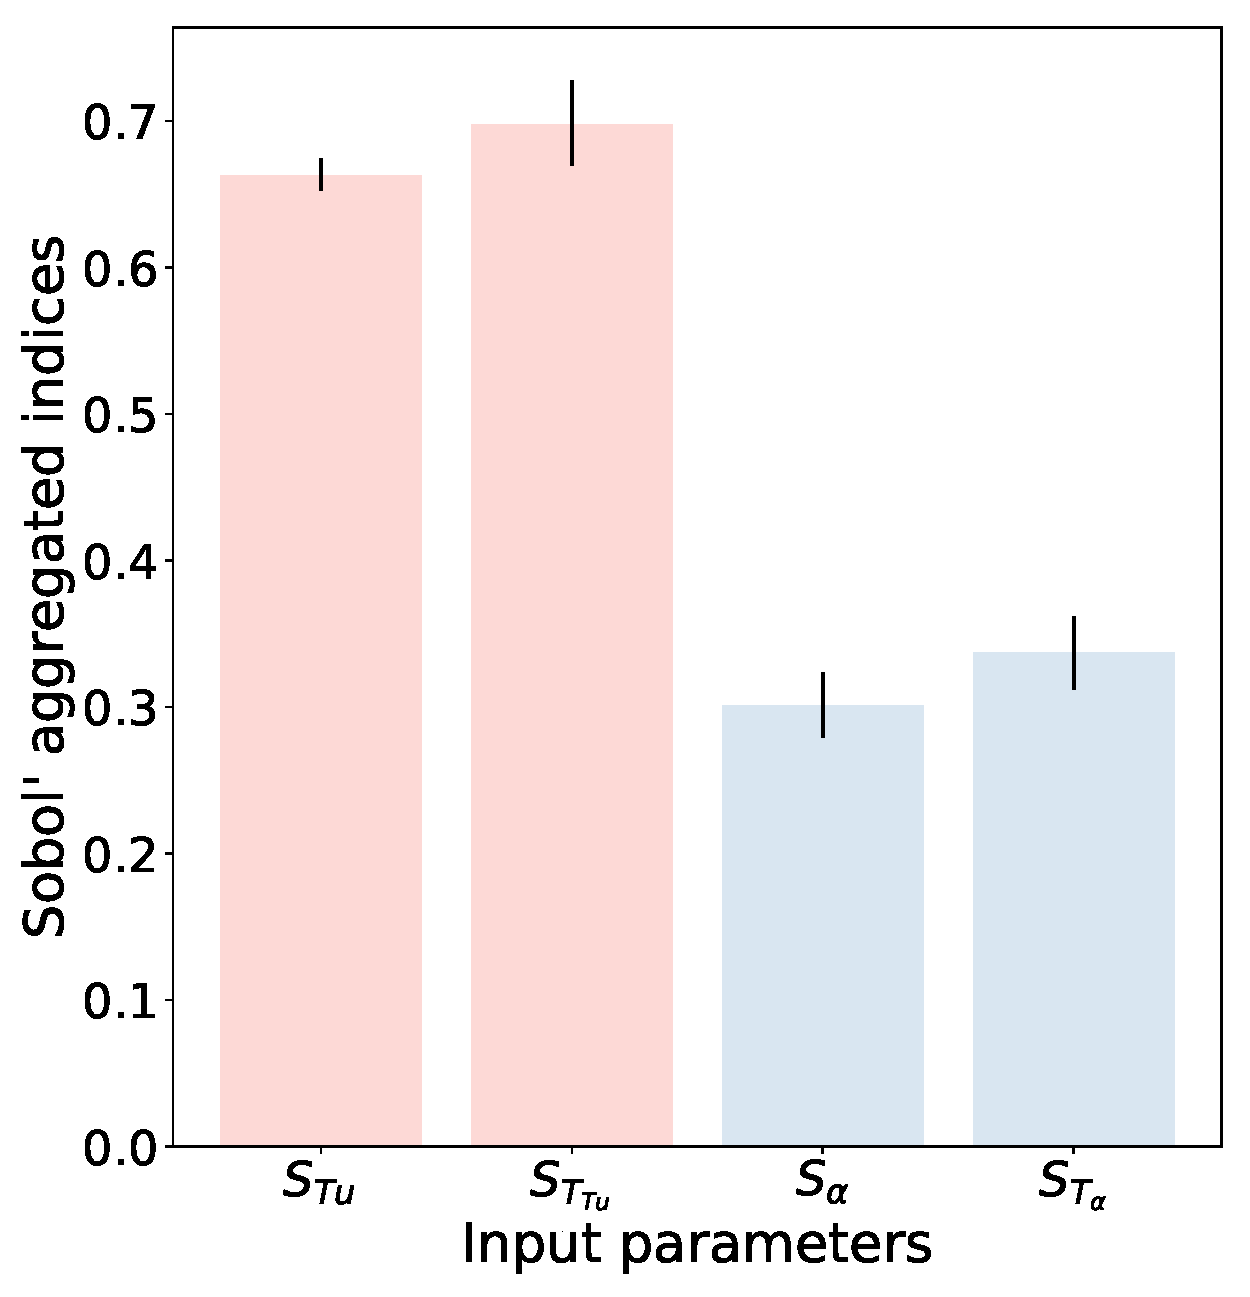
\includegraphics[width=0.5\linewidth]{fig/applications/ls89/15_1column_color-online-only_aggregated_indices.pdf}
\caption{Aggregated \textit{Sobol'} indices of the input parameters with their asymptotic confidence intervals.}
\label{fig:ls89-aggregated}
\end{figure}

The response surfaces of the models are plotted in \cref{fig:ls89-RS}. The heat transfer coefficient has been integrated over the chord line to obtain this visualization. The first thing to notice is the correct distribution of sample points within the parameter space ensuring that most of the effects are captured. The predictions obtained using the models are then found to be in agreement with the observations made previously. The heat transfer coefficient increases with the turbulence intensity and is fairly stable regarding the angle of the incoming flow. The models are said to be additive with respect to the turbulence intensity. Contrary to the \textit{Sobol'} sequence, the LOO-\textit{Sobol'} method detected that the model was sensitive to low values of turbulence intensity. It is this physical information that helped improve the predictivity quality. In the following, the model constructed using the LOO-\textit{Sobol'} method is used.

\begin{figure*}[!h]
\centering
\subfloat[\textit{Sobol'} sequence]{
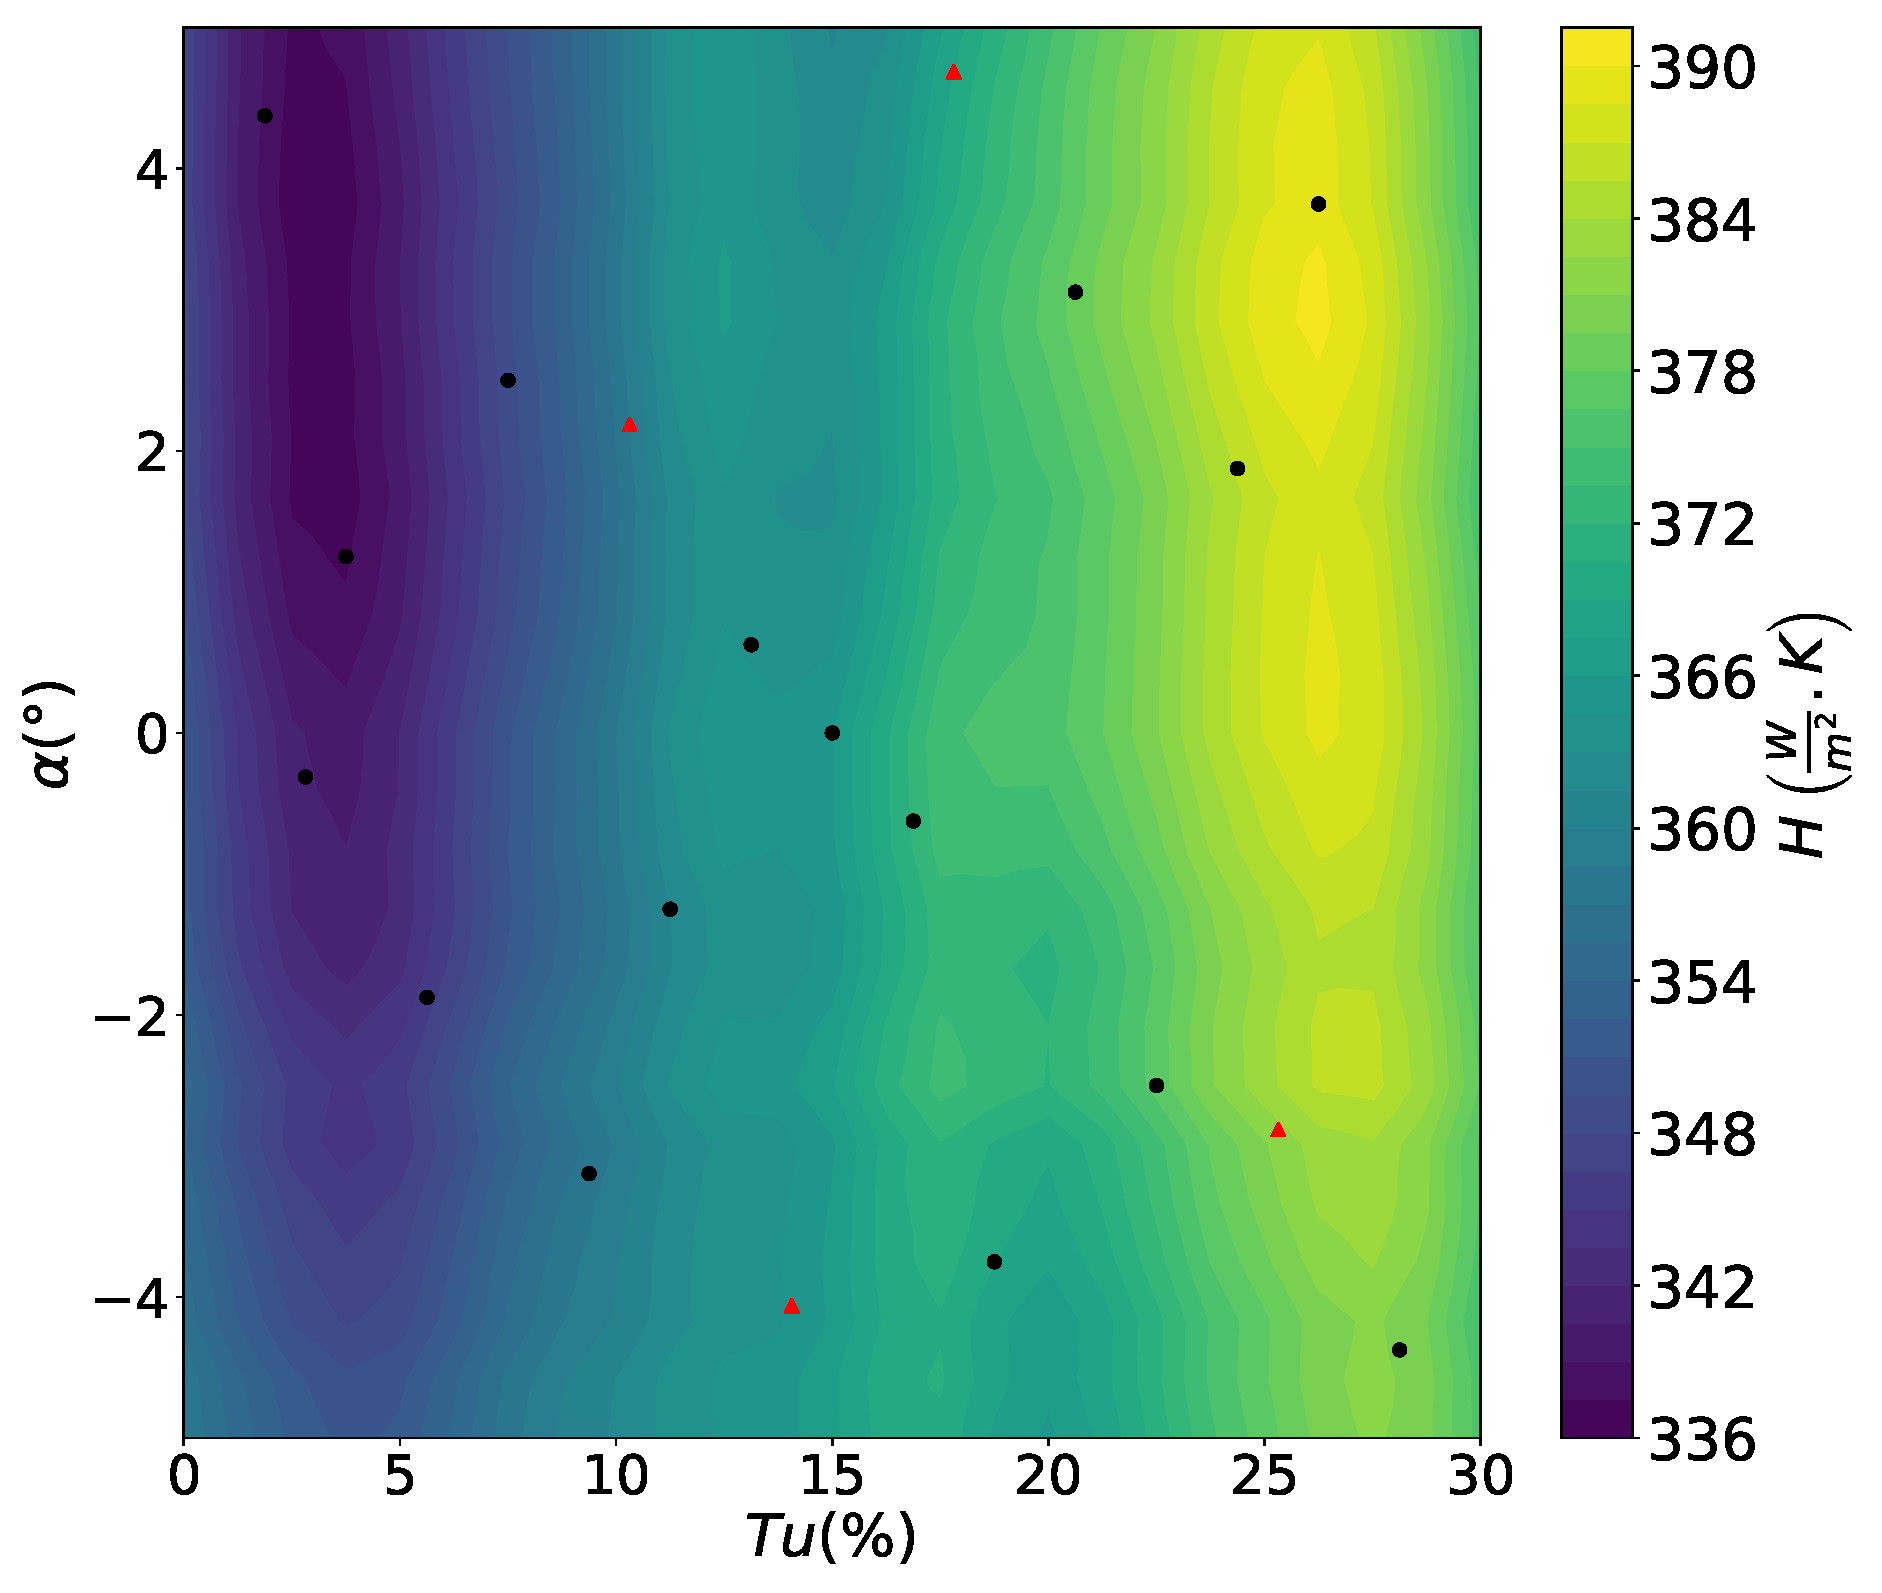
\includegraphics[width=0.4\linewidth,height=\textheight,keepaspectratio]{fig/applications/ls89/12a_2column_color-online-only_response_ls89_sobol.pdf}}
~
\subfloat[$\sigma$ method]{
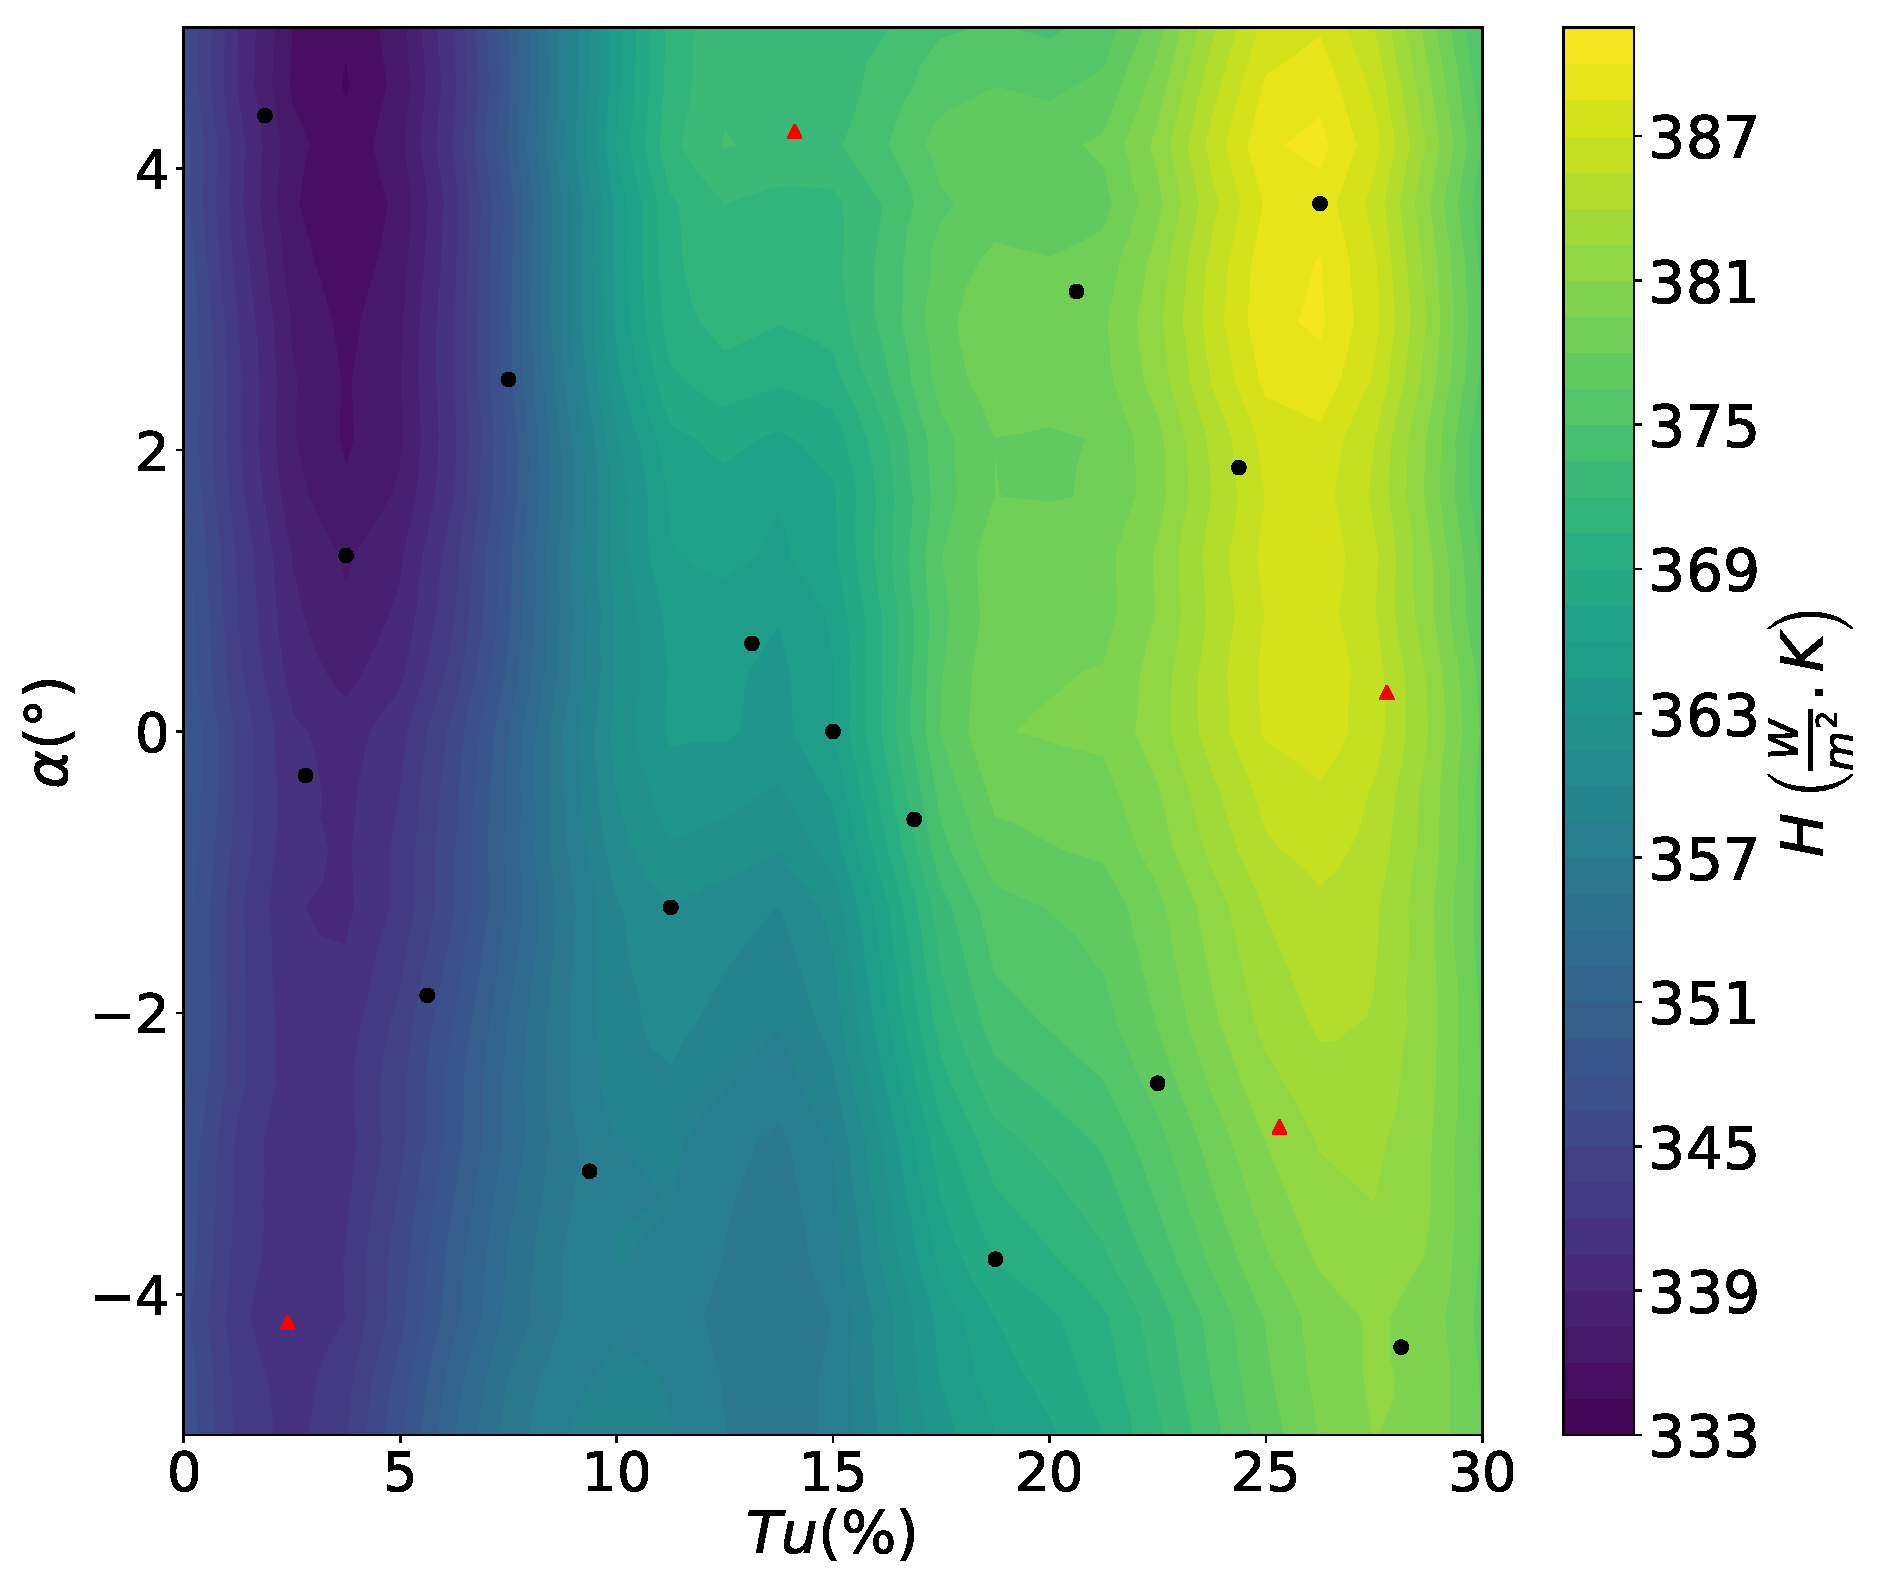
\includegraphics[width=0.4\linewidth,height=\textheight,keepaspectratio]{fig/applications/ls89/12b_2column_color-online-only_response_ls89_sigma.pdf}}

\subfloat[LOO-\textit{Sobol'} method]{
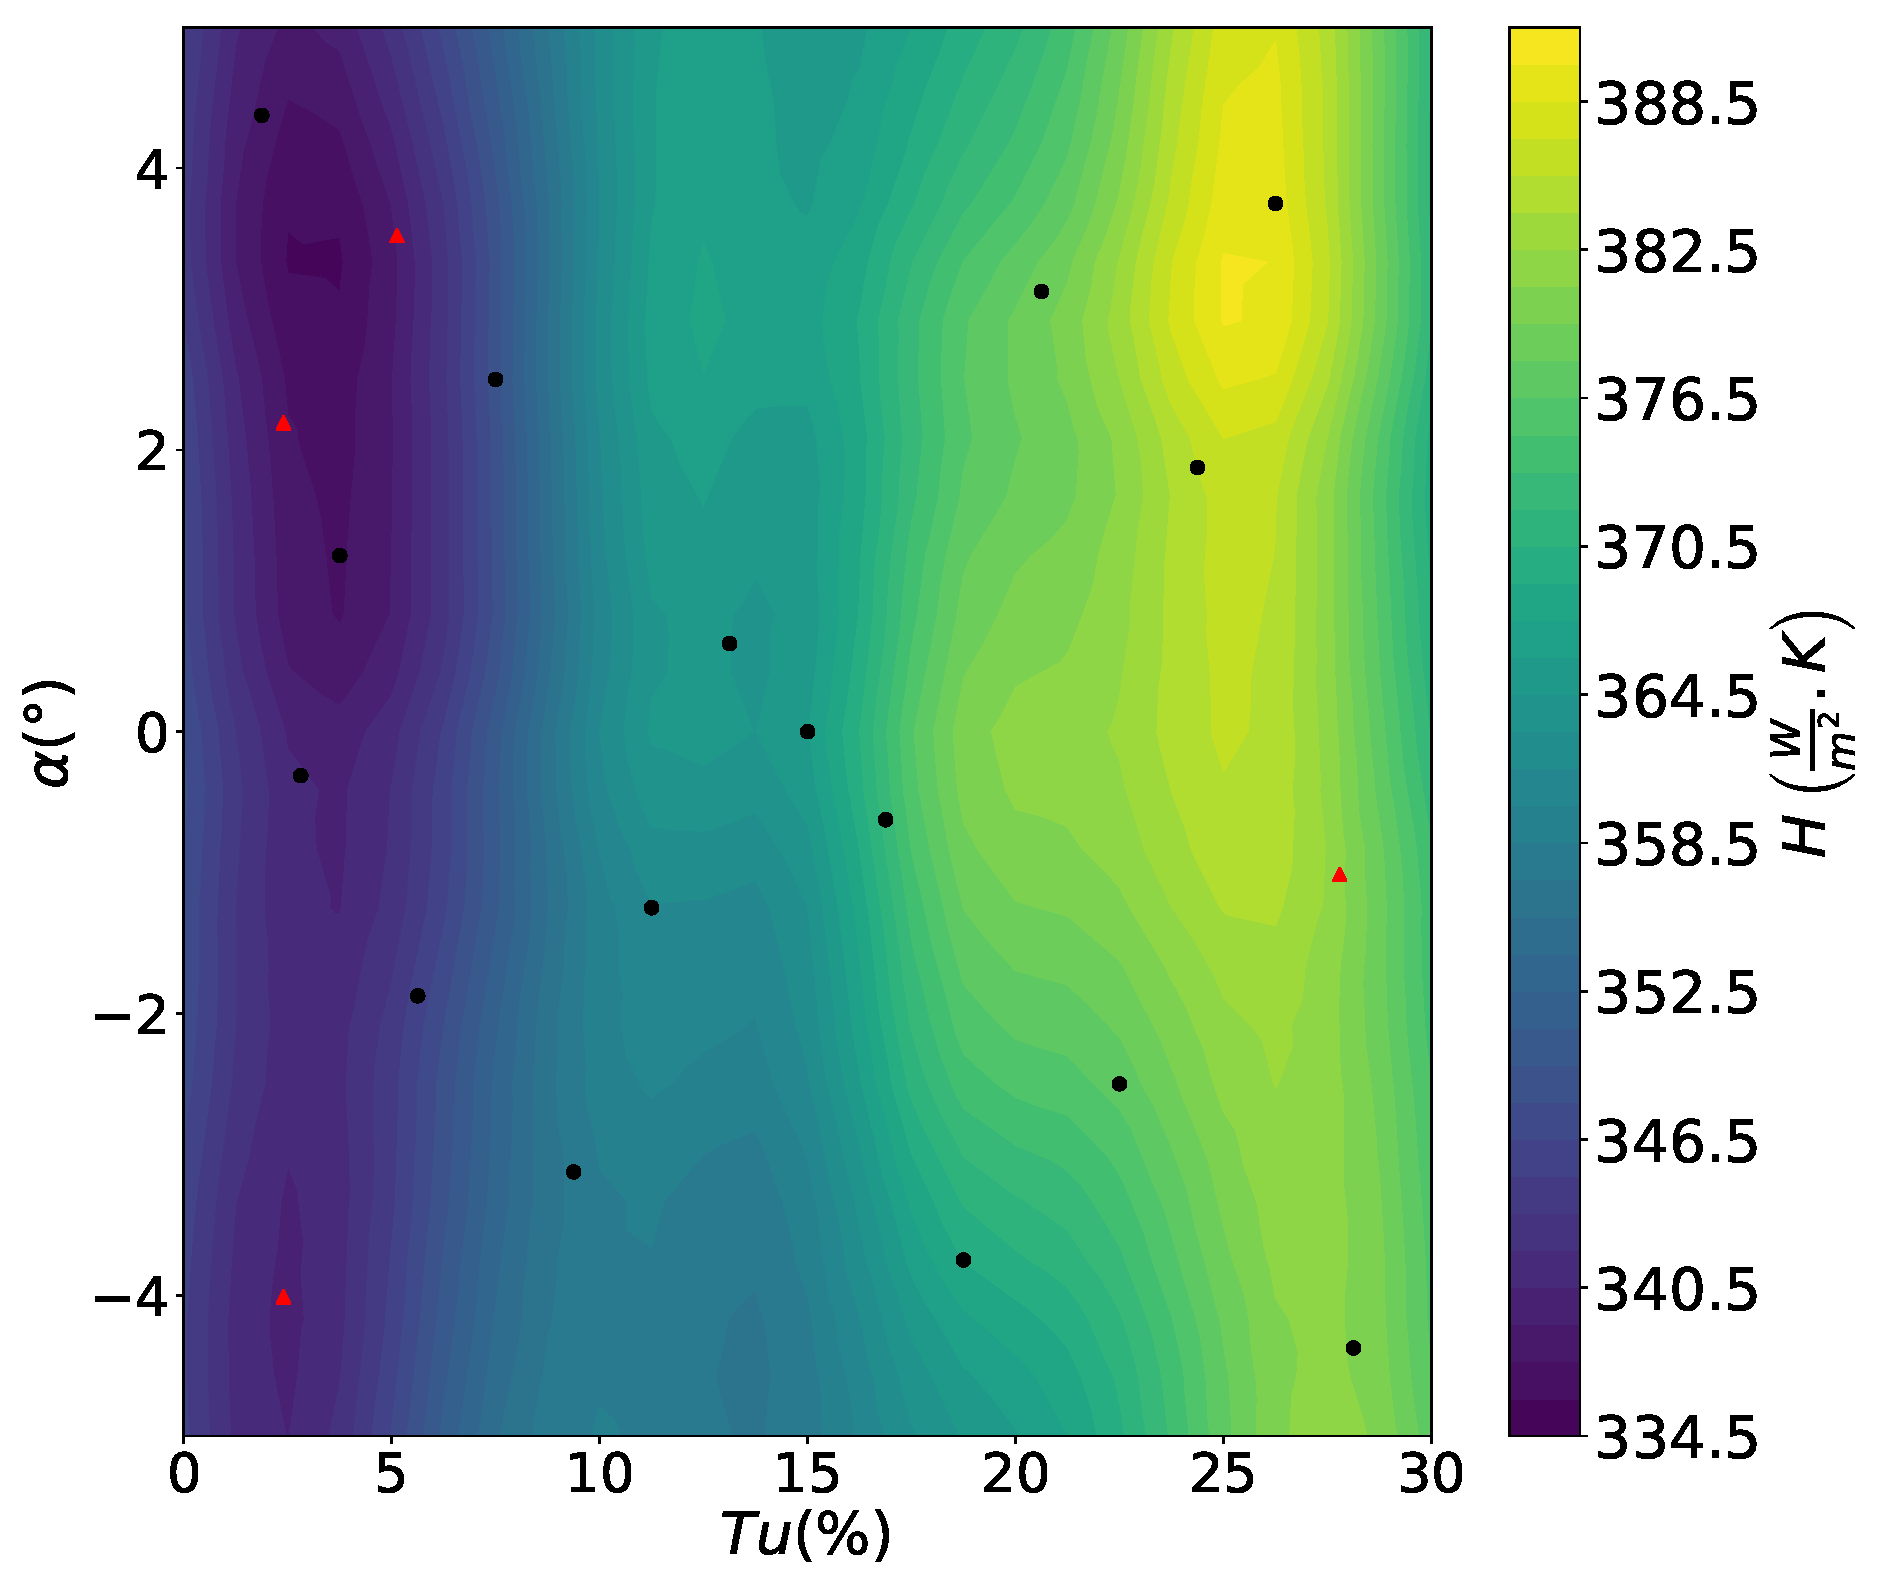
\includegraphics[width=0.4\linewidth,height=\textheight,keepaspectratio]{fig/applications/ls89/12c_2column_color-online-only_response_ls89_loo-sobol.pdf}}
\caption{Heat Transfer coefficient response surface. DoE is initially composed of 16 simulations sampled with \textit{Sobol'} sequence. Dots represent the initial LES simulations and diamonds represent the resampled points.}
\label{fig:ls89-RS}
\end{figure*}

Without making any assumption on the uncertainties, the Probability Density Functions (PDF) of the input parameters are both defined using uniform distributions over the parameter space
\begin{align}
Tu\sim \mathcal{U}(0,30\%) \quad \alpha \sim \mathcal{U}(-5,5\degree).
\end{align}
Using these PDFs, uncertainties are propagated by $\numprint{5000}$ predictions of the heat transfer coefficient along the blade. Then the QoI's PDF is reconstructed using a kernel smoothing procedure~\cite{wand1995,hastie2009}. \Cref{fig:ls89-propagation} reveals the expected concerning the propagation of such uncertainties to the heat transfer coefficient. As the two input distributions are uniform and the model is additive, the mean is centred between the extrema. From the experiments---see~\cref{fig:space-tu-alpha}---the envelope of the heat transfer coefficient is correctly captured except after the shock region. Indeed, from past experiences, capturing this region requires a value of $y^+\sim 1-2$~\cite{Segui2017b}.

\begin{figure*}[!h]
\centering
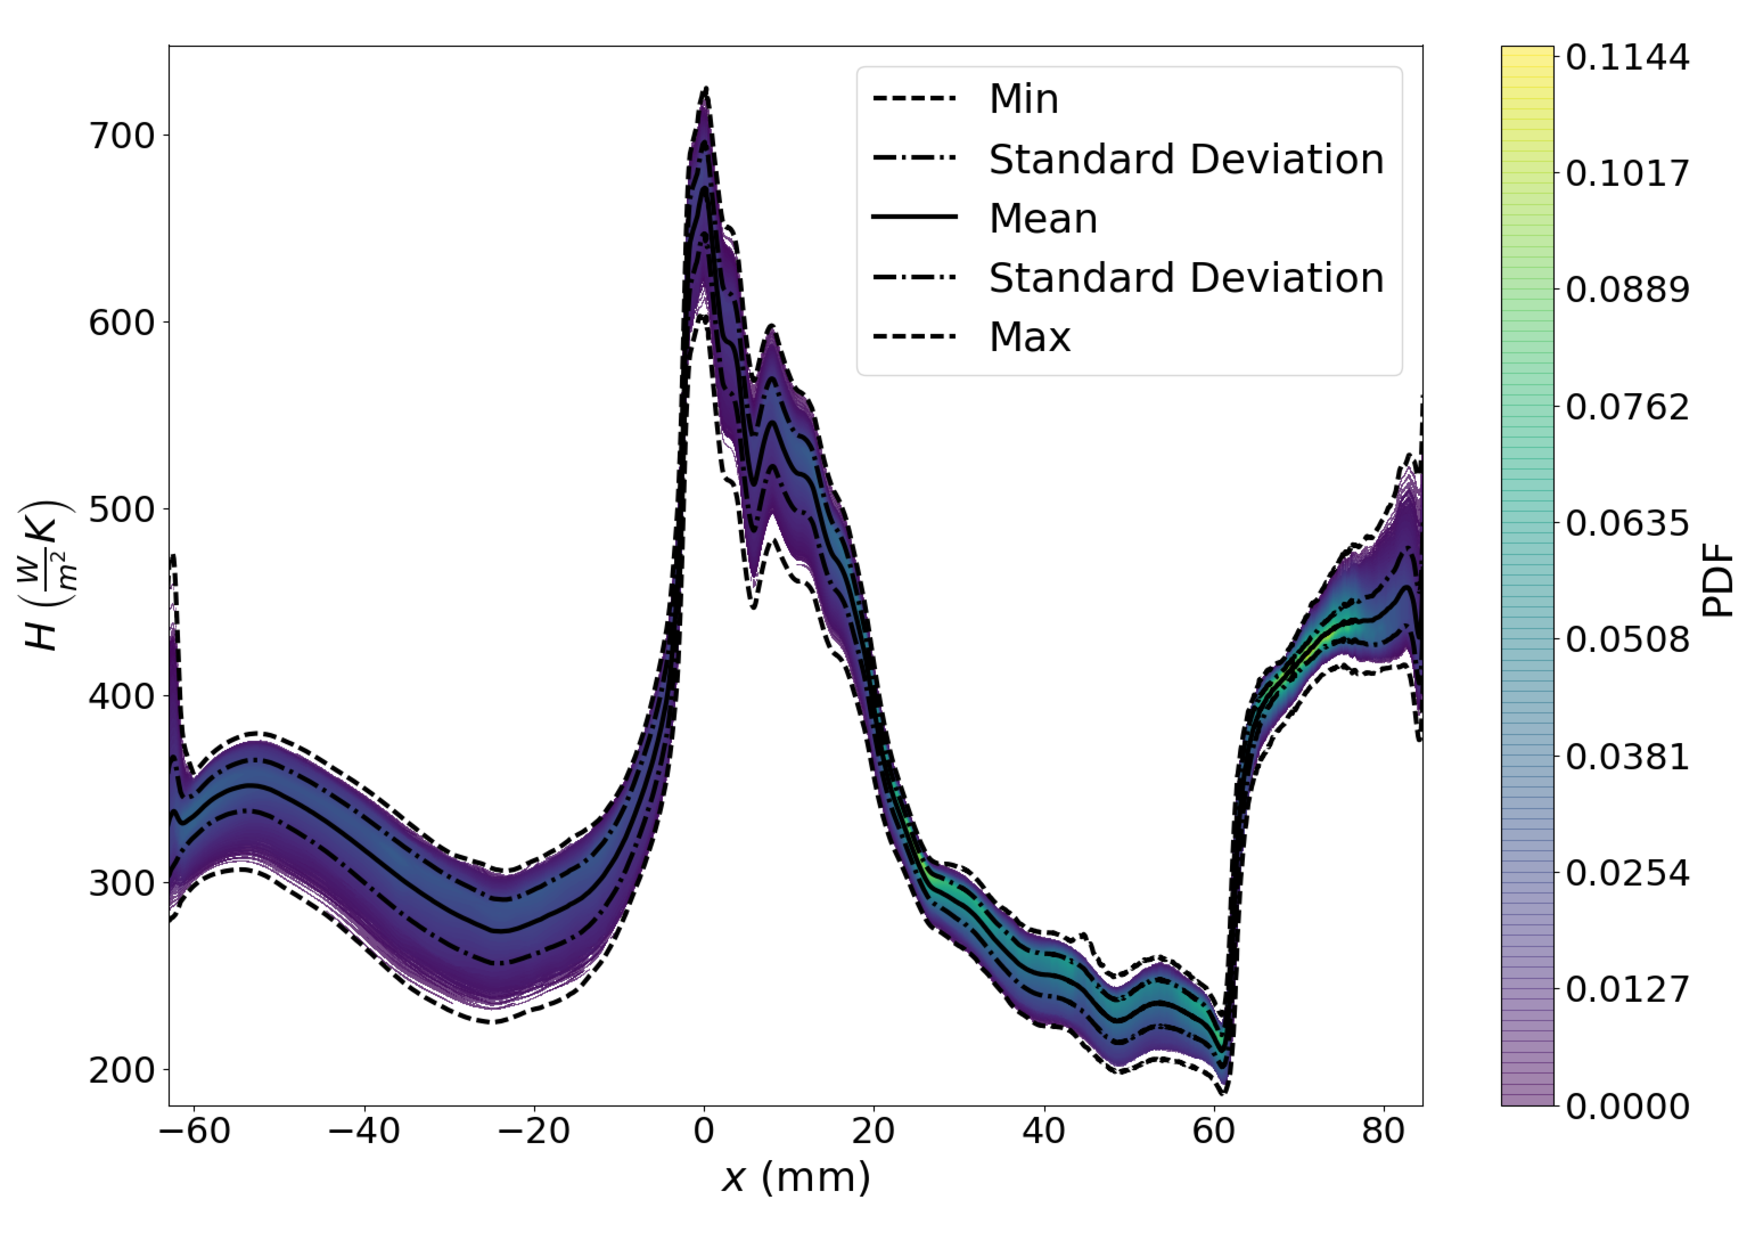
\includegraphics[width=0.7\linewidth]{fig/applications/ls89/13_2column_color-online-only_pdf-moments.pdf}
\caption{Probability Density Function and moments of the heat transfer coefficient along the chord line of the blade.}
\label{fig:ls89-propagation}
\end{figure*}

\begin{figure*}[h]
\centering
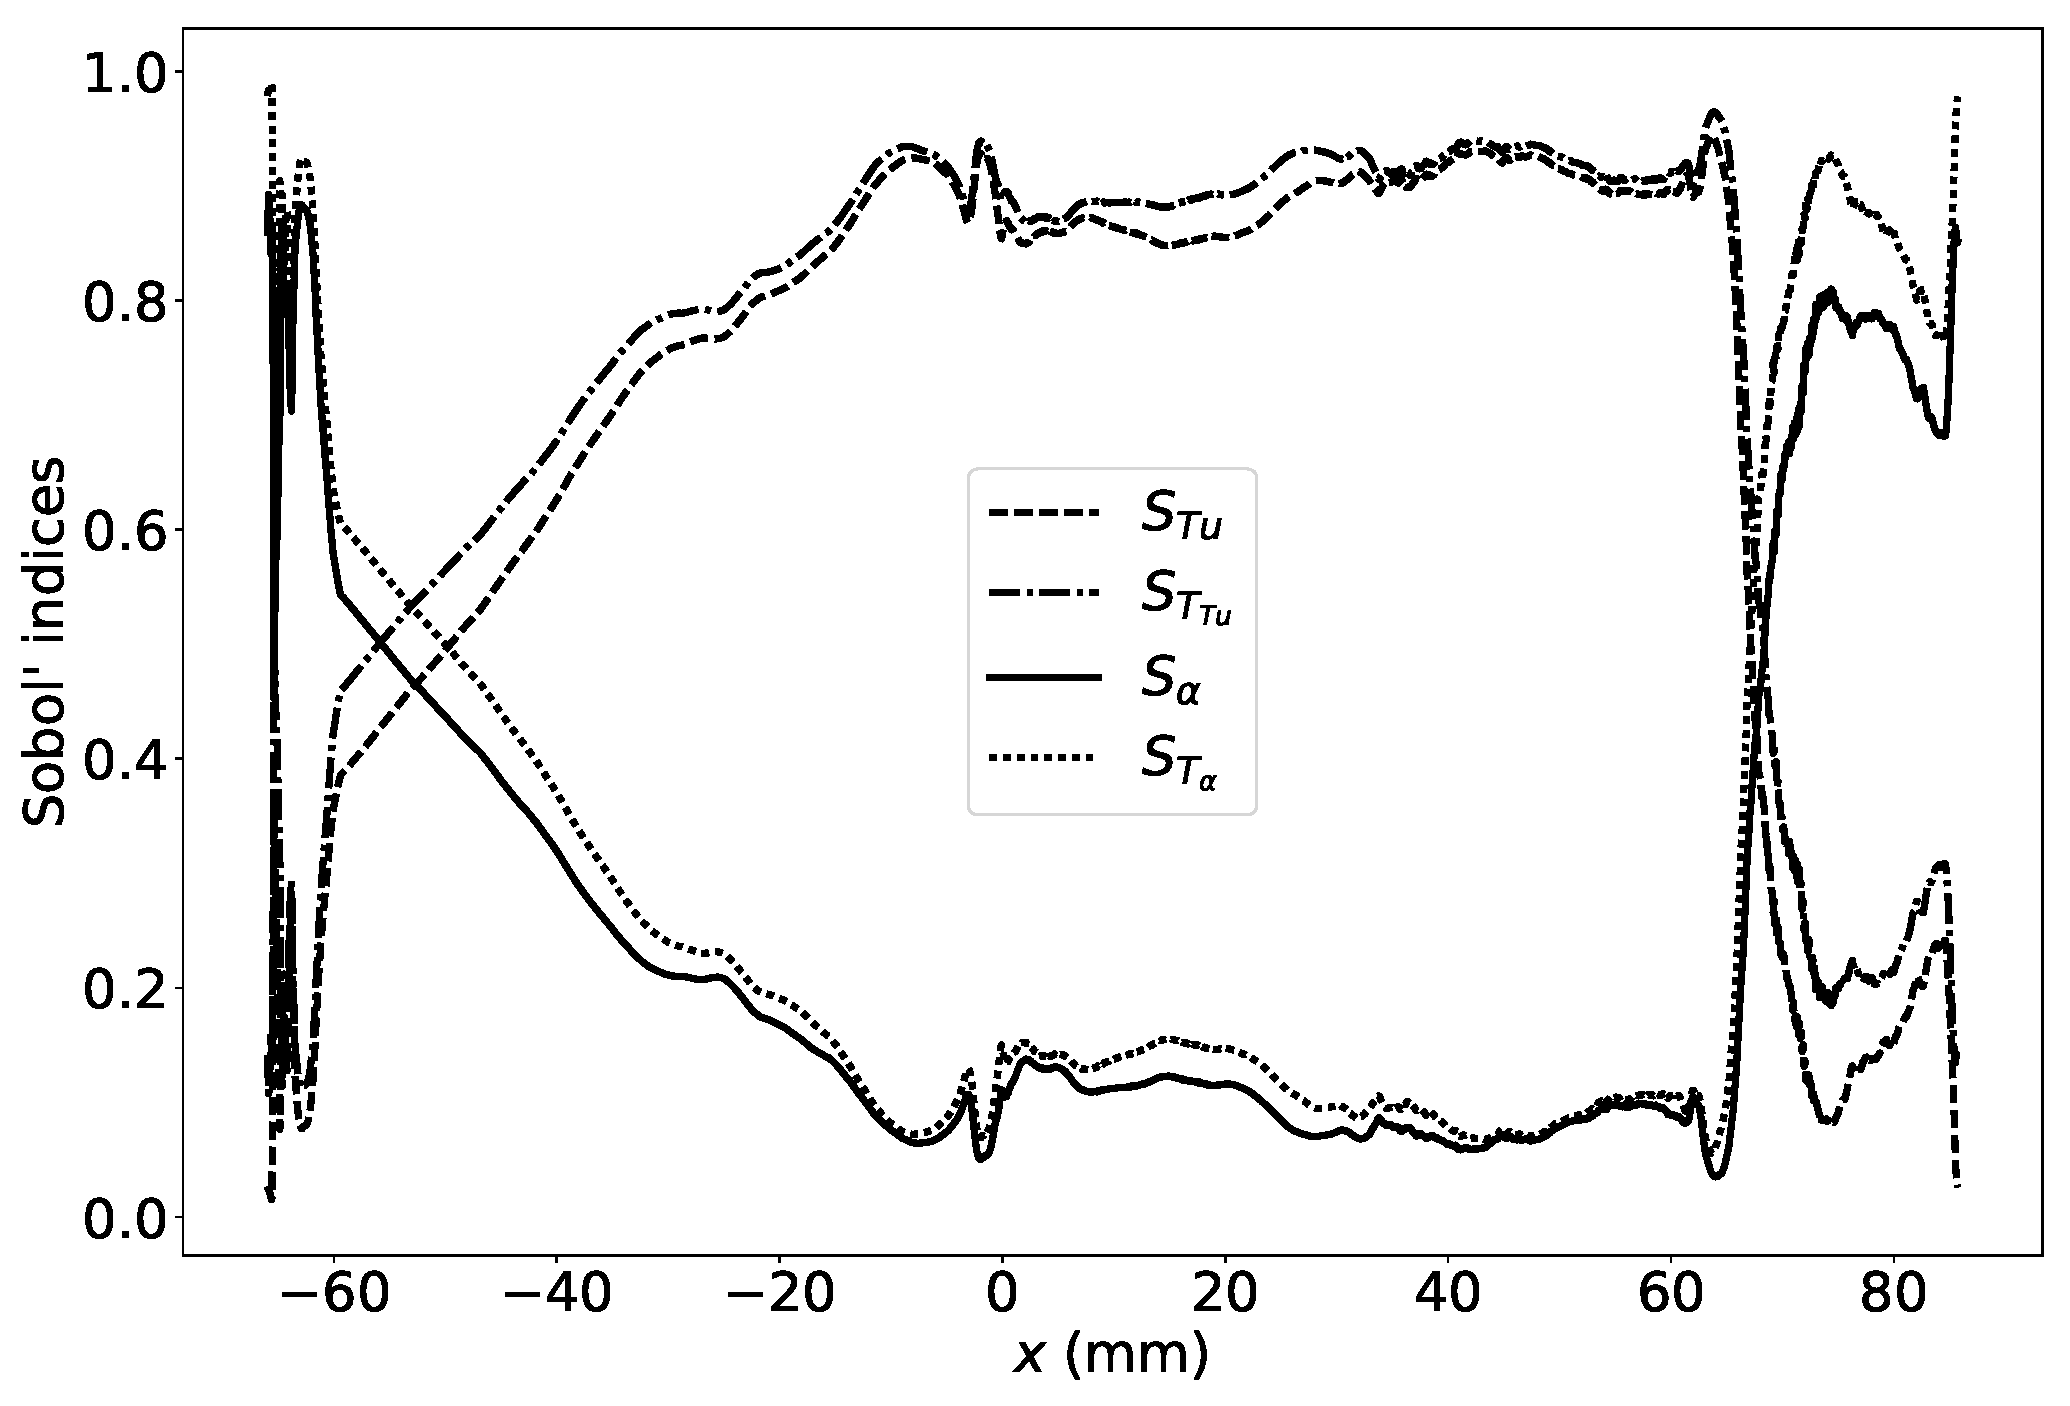
\includegraphics[width=0.7\linewidth]{fig/applications/ls89/14_2column_color-online-only_sensitivity_map.pdf}
\caption{First order and total order \textit{Sobol'} indices along the chord line.}
\label{fig:ls89-map}
\end{figure*}

Finally, the \textit{Sobol'} indices have been estimated using $\numprint{200000}$ predictions. As the response surface suggested, the heat transfer coefficient is mainly affected by the variation of the turbulence intensity. The spatial evolution of the indices in~\cref{fig:ls89-map} shows a spatial dependency. On the pressure side, the inflow angle has a higher influence as its contribution rises to become the most important parameter at the trailing edge. On the suction side, the turbulence intensity contribution is stable until the shock region. Reaching the trailing edge, the angle contribution increases. Finally, aggregated indices are reported in~\cref{fig:ls89-aggregated}. These indices confirm that the turbulence intensity is the most important parameter compared to the inflow angle when studying the heat transfer coefficient and for the range of angle variations retained. The turbulence intensity contributes to 70\% of the total variance of the QoI whereas the inflow angle contributes to 30\%. This behaviour was expected as downstream the shock, the incoming level of turbulence has little impact. The computation of the second order indices are not presented here because their values are negligible in comparison to the first order indices. This is in agreement with the small differences observed between the first and total order indices. There are no joint effects between the two parameters.


\section{Conclusion}\label{sec:ls89_ccl}

A first Uncertainty Quantification LES study of the \textit{LS89} is presented. The parameter space was comprised of the turbulence intensity and the inflow angle. In order to increase the quality of the surrogate model, the LOO-\textit{Sobol'} method was used to refine the parameter space. We showed that it performed better than continuing the sampling sequence. Apart from an analysis of the variance, the model was used to propagate uncertainties. This study reveals that although the turbulence intensity is the main factor impacting the heat transfer coefficient, there is spatial evolution of its contribution along the blade.


\chapter{Swirler}

\newcommand{\pdv}[2]{\frac{\partial{#1}}{\partial{#2}}}
\newcommand{\tilda}[1]{\tilde{#1}}

\section{Introduction}\label{sec:intro}

At the heart of a turbomachine is the combustion chamber, fed with fuel by injectors. Here, the combustion process releases the calorific capacity of the fuel mixture. This process is usually started using a spark which provides an energy deposit in the system. After the flame has been ignited, it needs a mechanism for it to stabilize within the chamber. Depending on the velocity of the laminar flame speed and on the power required, different devices are to be considered to stabilized a flame. Indeed, the output power being directly linked to the inlet velocity of the reactants, if a high power is required, the inlet velocity will be high. Thus, to stabilize the flame ones needs to equilibrate the consumption of the reactants accordingly to the flame speed. The flame stabilization is a major concern which can cause an extinction of the chamber or an oscillation of the flame.

 When considering small velocities, a backward facing step is sufficient---see~\cref{fig:sketch-step}. This geometry creates a recirculation zone that traps the fuel mixture downward. However, as the inlet velocity increases, the flame speed does not. The chemistry not being infinitely fast, comes a point were the flame cannot sustain. Swirled injectors have been designed to overcome this issue~\cite{Lilley1977}---see~\cref{fig:sketch-swirler}. By impinging a movement of rotation on the flow, a recirculation zone is created directly at the outlet of the injector. This ensures sufficient residence time for the fuel to be consumed. The design of swirled injectors is of prime importance when seeking to reduce fuel consumption and pollutant emissions. Indeed, this is usually achieved via lean combustion which may lead to combustion instabilities and reduced extinction margins. When considering environmental aspects, operability, efficiency, maintenance or even durability, the problem becomes a complex multiobjective optimization problem which remains a great challenge.

\begin{figure}[!h]
\centering
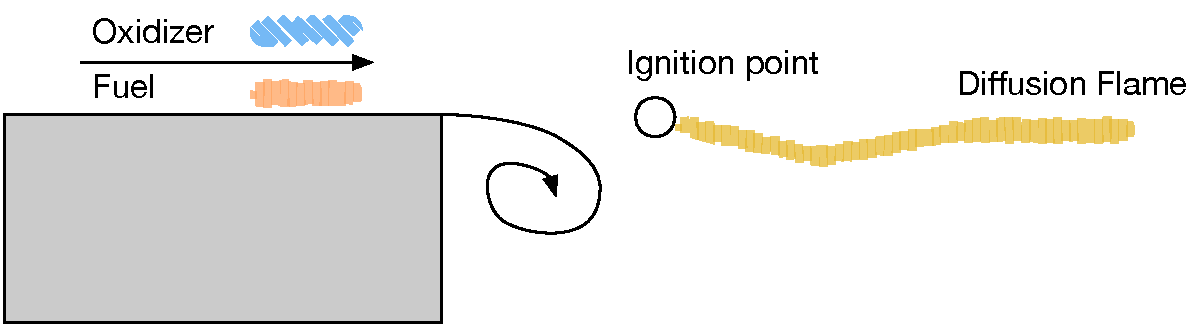
\includegraphics[width=\linewidth,keepaspectratio]{fig/applications/swirler/sketch_step.pdf}
\caption{Sketch of a backward facing step.}
\label{fig:sketch-step}
\end{figure}

\begin{figure}[!h]
\centering
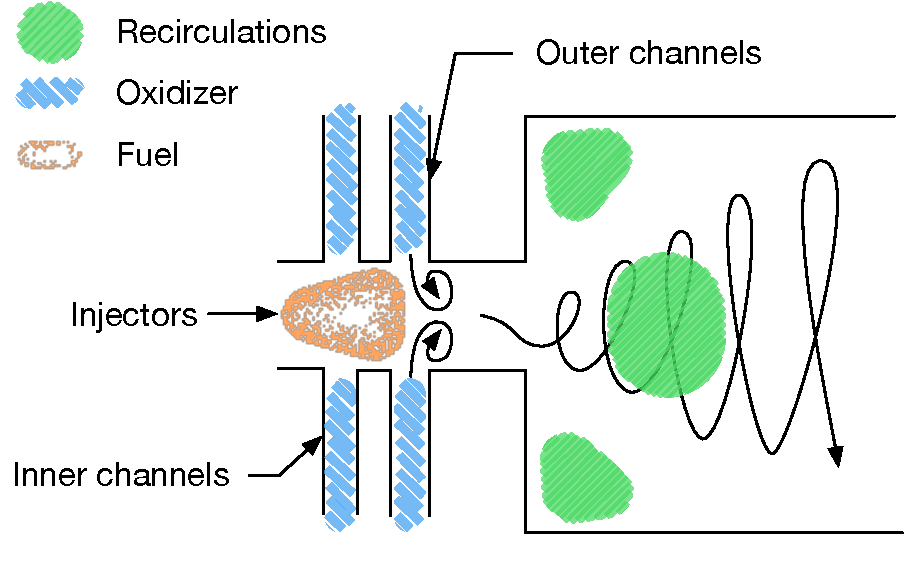
\includegraphics[width=\linewidth,keepaspectratio]{fig/applications/swirler/sketch_swirler.pdf}
\caption{Sketch of a swirler consisting of two contra-rotative sets of oxidizer channels.}
\label{fig:sketch-swirler}
\end{figure}

To help in the development of future engines, numerical simulations---and here Computational Fluid Dynamics (CFD) simulations---, have undoubtedly become reliable and essential design tools~\cite{Sacks1989,Forrester2009}. Recently, the use of Large Eddy Simulations (LES) coupled with a mesh adaptation strategy has demonstrated its capacity to identify the relevant physics of swirling flows \cite{Daviller2017}. % TODO Complete
From expert knowledge, the design of a swirler proceeds in three steps: (\emph{i})~an exploratory phase is first performed using Reynolds-averaged Navier-Stokes (RANS) computations; (\emph{ii})~the resulting possible geometries installed in the combustion chamber are simulated using LES of turbulent combustion; (\emph{iii}) prototypes are manufactured and tests are performed. The first step allows to explore a large range of possibilities in terms of geometrical modifications (angles, number of channels, etc.) to meet requirements such as the swirl number, effective surface and permeability. The second step is performed to assess the combustion stability and the combustor performances in various operating conditions. Finally experiments are conducted to finalize the design.

For this last step, metal Additive Manufacturing (AM)~\cite{Frazier2014,Sames2016} is now in use. The AM technology has gained a lot of attention as it does not impose any constraint from the design point of view without sacrificing mechanical properties~\cite{Lewandowski2016}. However, AM induces some uncertainties regarding the structural composition of the produced metallic systems, making this an active topic of research. In particular, geometrical uncertainties may result from the deposition method, the scanning method or even the powder size. Moreover, due to the complexity of some designs, it might not be possible to polish surfaces using standard mills. This may leave some defects which size depends on the quality of the whole process.

The present study aims to measure the effect of AM on the fluid motion. This is achieved through Uncertainty Quantification (UQ)~\cite{Iooss2015a} based on LES with varying geometry. A Principal Component Analysis (PCA) is first performed to build a reduced parameter space allowing to take into account all design variables. Then, uncertainties on the design variables are propagated in a series of 30 LES, providing summary statistics.

The chapter is organized as follows: \cref{sec:swirler} presents the studied configuration as well as the LES numerical setup. \Cref{sec:dim} details the methodology used to reduce the parameter space. Results of the UQ study are then presented and analyzed in  \cref{sec:res} and \cref{sec:disc}, respectively.

\section{Configuration and Numerical Setup}\label{sec:swirler}

\subsection{The Swirled Injector}

\Cref{fig:scheme-swirler} presents a sketch of the swirler studied in this work (also described in \cite{Daviller2017}) together with the computational domain. The swirler consists of two counter-rotating stages of 8 tangential vanes resulting in a rotational flow. A recirculation zone appears just downstream the swirler, which is paramount to combustion stability. In this study, no fuel is injected.

\begin{figure}[!ht]
\centering
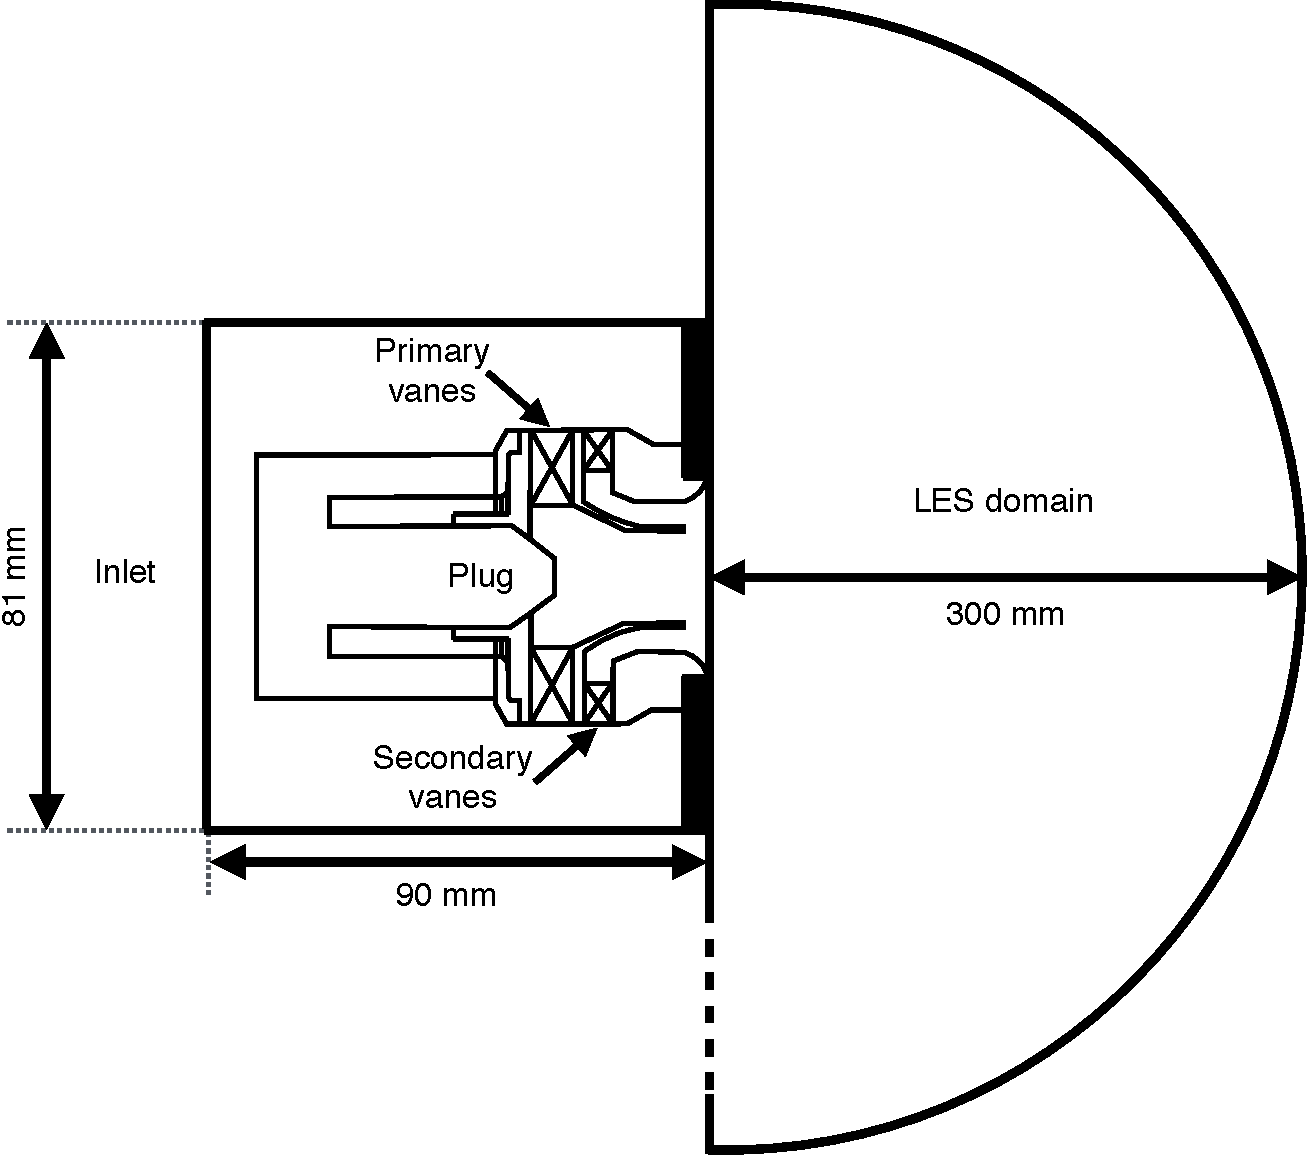
\includegraphics[width=0.8\textwidth,keepaspectratio]{fig/applications/swirler/swirler_UQ.pdf}
\caption{Schematic view of the configuration and the LES computational domain.}
\label{fig:scheme-swirler}
\end{figure}

\subsection{Numerical Setup} \label{sec:num_setup}

All simulations were performed using the compressible Navier-Stokes solver AVBP~\cite{sch1999steady}. The finite-element scheme TTGC~\cite{colin_JCP_2000} was used on a tetrahedral mesh and LES equations were closed using the $\sigma$-model~\cite{nicoud_PoF_23_2011}. At the inlet and outlet boundaries Navier-Stokes Characteristic Boundary Conditions (NSCBC) were applied~\cite{poinsot1992boundary}, imposing the mass flow rates and the pressure, respectively. All wall boundary conditions were specified as wall no-slip conditions without wall law models.

\subsubsection{Mesh Adaptation Strategy}
Due to the relative complexity of the geometry and the resulting mesh size, an Adaptive Mesh Refinement (AMR) strategy was used to reduce the CPU cost while preserving the quality of the solution, evaluated with the global pressure loss $\Delta P$. The AMR strategy used in this study is based on the methodology proposed in~\cite{Daviller2017}: from the result obtained on an initial arbitrary mesh, a metric based on the time-averaged viscous dissipation field $\mathrm{\overline{\Phi}}$ is computed as: 
\begin{equation}\label{eq:phi}
\mathrm{\overline{\Phi}} = \overline {( \mu + \mu_t) \left(\pdv{u_i}{x_j} + \pdv{u_j}{x_i}\right)^2 },
\end{equation}
where $\mu$ is the molecular viscosity and $\mu_t$ the turbulent viscosity.\\
Then the mesh of the computational domain is adapted using the MMG3D library~\cite{Dapogny2014358}(noted \emph{AD1}). This procedure is repeated with a second adaptation (noted \emph{AD2}), so that the experimental pressure loss $\Delta P$ is recovered (see~\cref{pressure_drop_evolution}). The computational details of one adaptation run are summarized in~\cref{tab:summary-mesh}. In the end, with two mesh adaptation steps, one run required $\unit{\numprint{25000}}{CPU\;hours}$ to simulate $\unit{\numprint{40}}{\milli\second}$ of physical time.

\begin{figure}[!h]
\centering
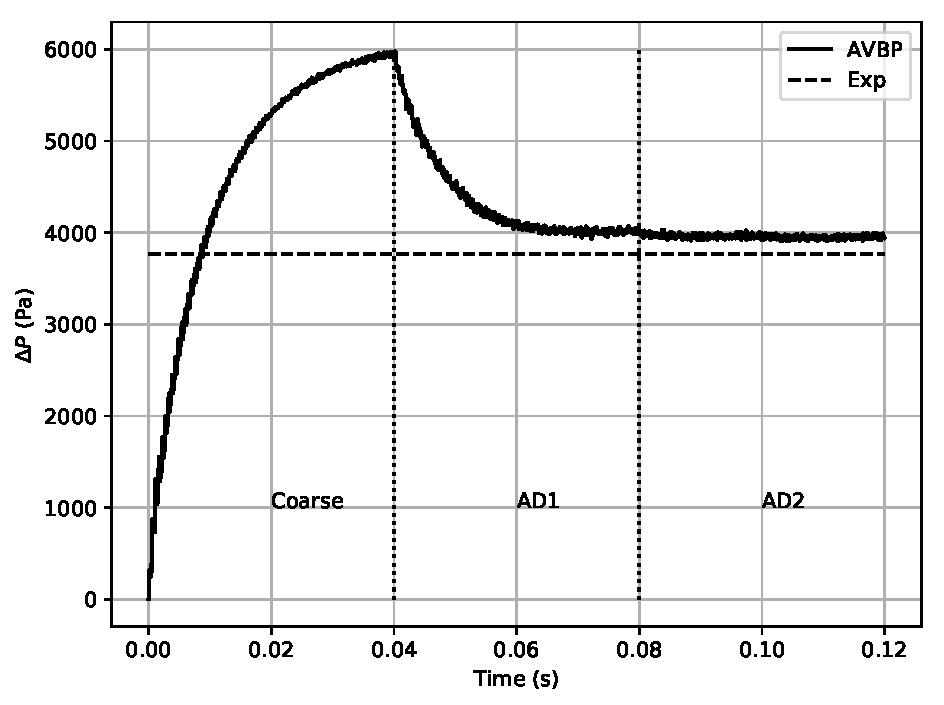
\includegraphics[width=\linewidth,keepaspectratio]{fig/applications/swirler/losses_swirler_base.pdf}
\caption{Evolution of the pressure loss computed with LES on the three different meshes successively with increasing resolution: \emph{Coarse}, \emph{AD1} and \emph{AD2}. The dash line represents the experimental value of $\Delta P$.}
\label{pressure_drop_evolution}
\end{figure}

% TODO définir epsilon et alpha

\begin{table}[!h]
\centering
\caption{Summary of mesh adaptation for one simulation. Physical simulation time is constant at $\unit{\numprint{40}}{\milli\second}$.}
\begin{tabular}{lccc}
\toprule
 & Coarse & AD1 & AD2  \\
\cmidrule{2-4}
%$\alpha$& - &50 & 30 \\
%$\epsilon$& - &0.3 & 0.4\\
number of cells ($\times10^6$) & 1.6 & 4.1 & 12.8 \\
time step ($\unit{\times10^{-7}}{\second}$) & 0.59 & 0.47 & 0.20\\
CPU hours & 5h30 & 2h20 & 9h30 \\
number of cores & 560 & 2800 & 2800 \\
$\Delta P$ relative error & $\unit{\numprint{57.8}}{\%}$ & $\unit{\numprint{6.5}}{\%}$ & $\unit{\numprint{4.8}}{\%}$\\
\bottomrule
\end{tabular}
\label{tab:summary-mesh}
\end{table}
% slurm-3106838.out | slurm-3154304.out | slurm-3156977.out

As shown in~\cite{Daviller2017}, this method converges and finally recovers the physics with a limited error on the pressure loss ($\sim 5$\%). This is obtained thanks to the choice of the viscous dissipation---which controls the irreversible losses---as the refinement metric. From~\cref{fig:mesh-AD-1-2} showing the evolution of the mesh, it appears that the mesh has mostly been refined around the plug tip and at the swirler exit. These zones indeed correspond to the zones where the dissipation is highest as seen in~\cref{fig:swirler_mod_phi}. This result also indicates that any geometrical deviation in these zones may result in a modified pressure loss. %Hence the ability of this mesh to correctly capture the fluid's features.

\begin{figure*}[!h]
\centering
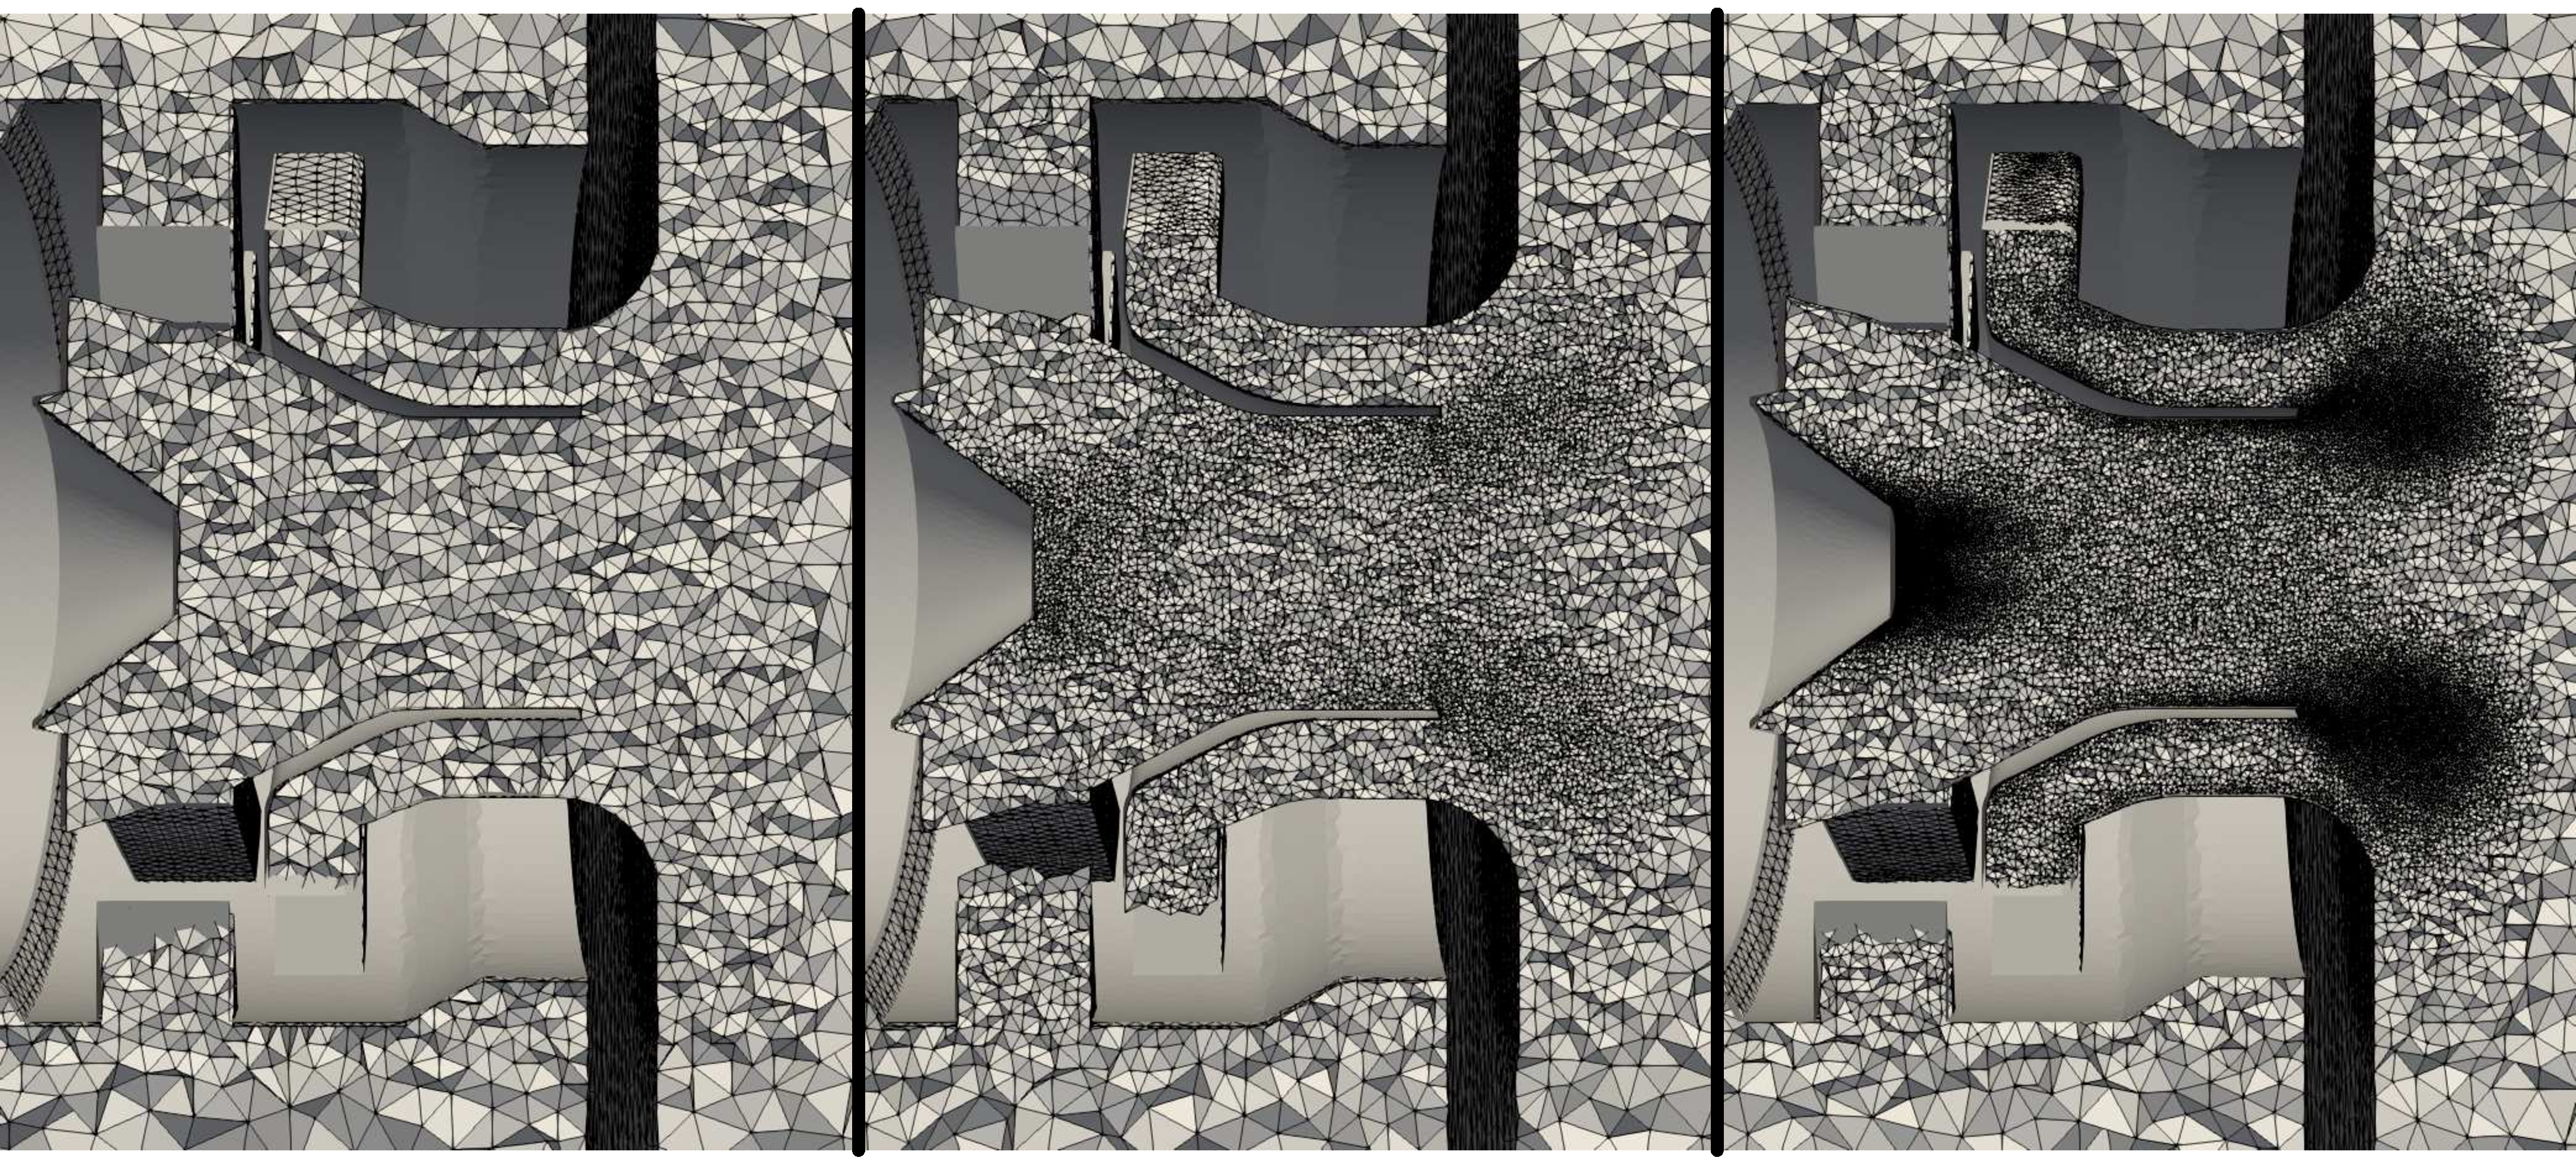
\includegraphics[width=\linewidth,keepaspectratio]{fig/applications/swirler/mesh_init-AD_1-2.pdf}
\caption{From left to right: coarse mesh, first adaptation \emph{AD1} and second adaptation \emph{AD2}.}
\label{fig:mesh-AD-1-2}
\end{figure*}


\subsubsection{Simulation Strategy for UQ}

In order to quantify the uncertainty on the flow physics, a sample of 30 LES was considered. The procedure used to generate this sample is detailed in~\cref{sec:dim}. For each simulation, a new geometry has been constructed with up to $2\%$ of variation in all channel dimensions---using the method presented in~\cref{sec:dim}. Then, the mesh was automatically adapted using the aforementioned methodology. This procedure ensures that the meshes are optimum for each configuration, with respect to the pressure loss. For the uncertainty analysis, results were averaged over $\unit{\numprint{40}}{\milli\second}$. The total computational cost for this UQ using LES is about $\unit{\numprint{1000000}}{CPU\;hours}$. Thanks to high performance computing resources, the return time was only 2 days, which is satisfactory in the context of an industrial design process.

Batman~\cref{chap:batman} was used to handle all simulations and perform the analysis.

\subsection{Geometrical Uncertainties of the Swirler}

Discrepancies in the size of the channels generated by AM have been measured. \Cref{fig:swirler_mod_phi,fig:swirler_mod_u} illustrate how a change of $\sim2$\% in all channel dimensions---due to manufacturing dispersion---impacts the flow and the pressure loss $\Delta P$. The two cases correspond to the maximum (case a) and minimum (case b) impact on the pressure loss. These results were obtained from LES and the numerical setup described in~\cref{sec:num_setup}.
\Cref{fig:swirler_mod_phi}~shows the difference in total dissipation field $\mathrm{\overline{\Phi}}$, which explains the difference in pressure drop.%, found here of $\sim5$\% between the two cases. 
Compared to the pressure drop in the reference geometry, the two cases show a difference of $7.83\%$ and $9.95\%$ respectively for~\cref{fig:swirler_mod_phi}(a) and~\cref{fig:swirler_mod_phi}(b). 
A closer look allows to identify the main region of difference at the tip of the plug, directly related to the flow difference in the first stage of the swirler, as seen in~\cref{fig:swirler_mod_u,fig:swirler_mod_u_3d}. Indeed, a small recirculation zone (at the tip of the plug) appears in the left case (a), which almost disappears in the right case (b).

\begin{figure}[!h]
\centering
        \subfloat[$\Delta P \sim \unit{\numprint{4020}}{\pascal}$]{
                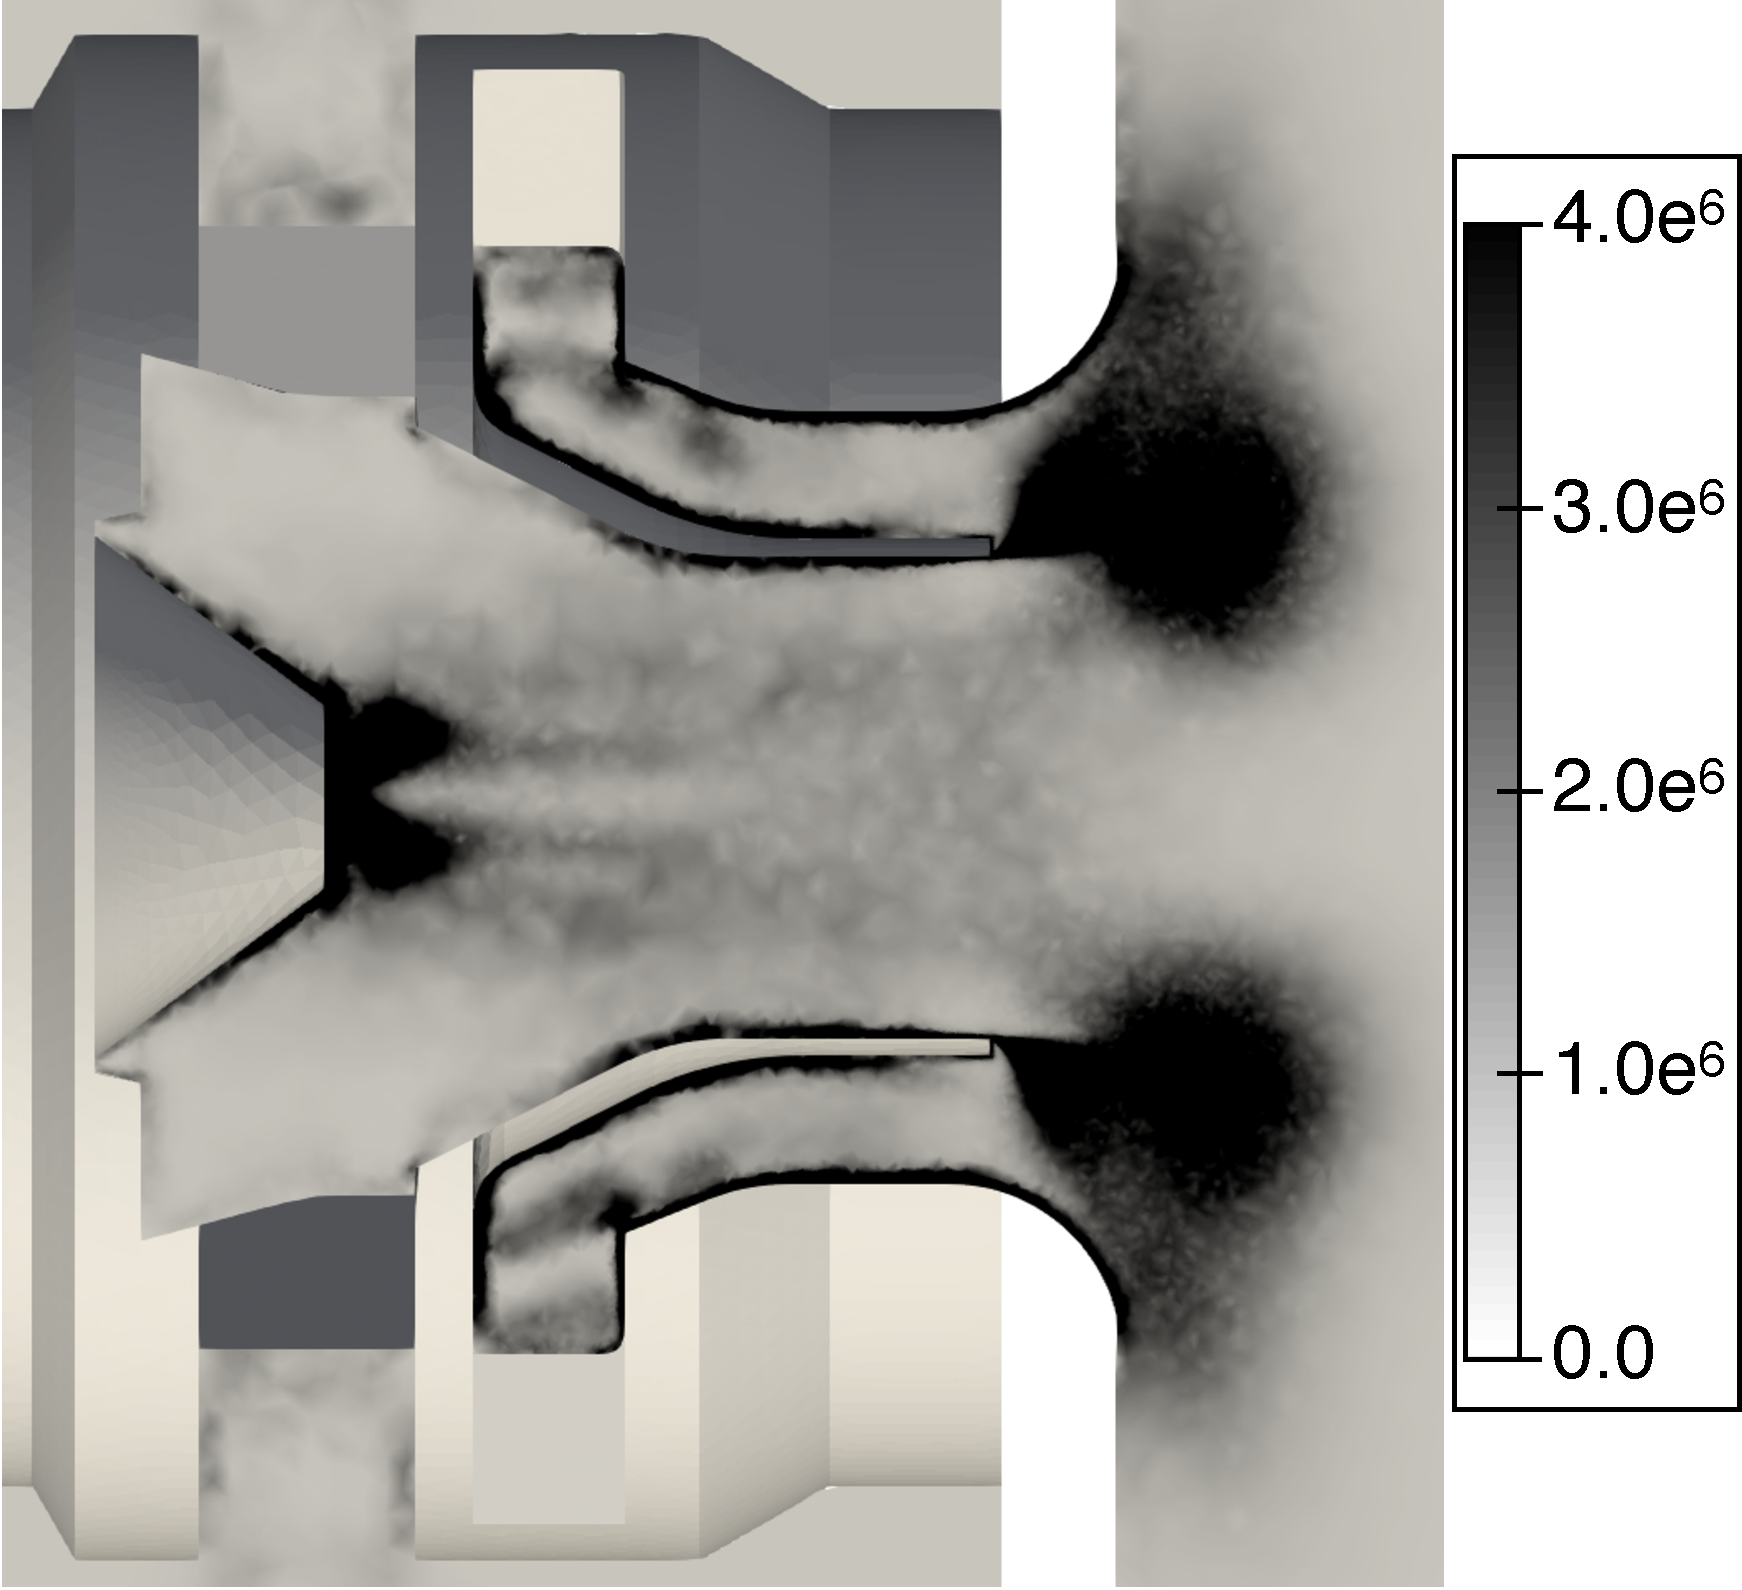
\includegraphics[width = 0.49\textwidth]{fig/applications/swirler/LikeMin}
        }
        \subfloat[$\Delta P \sim \unit{\numprint{4260}}{\pascal}$]{
                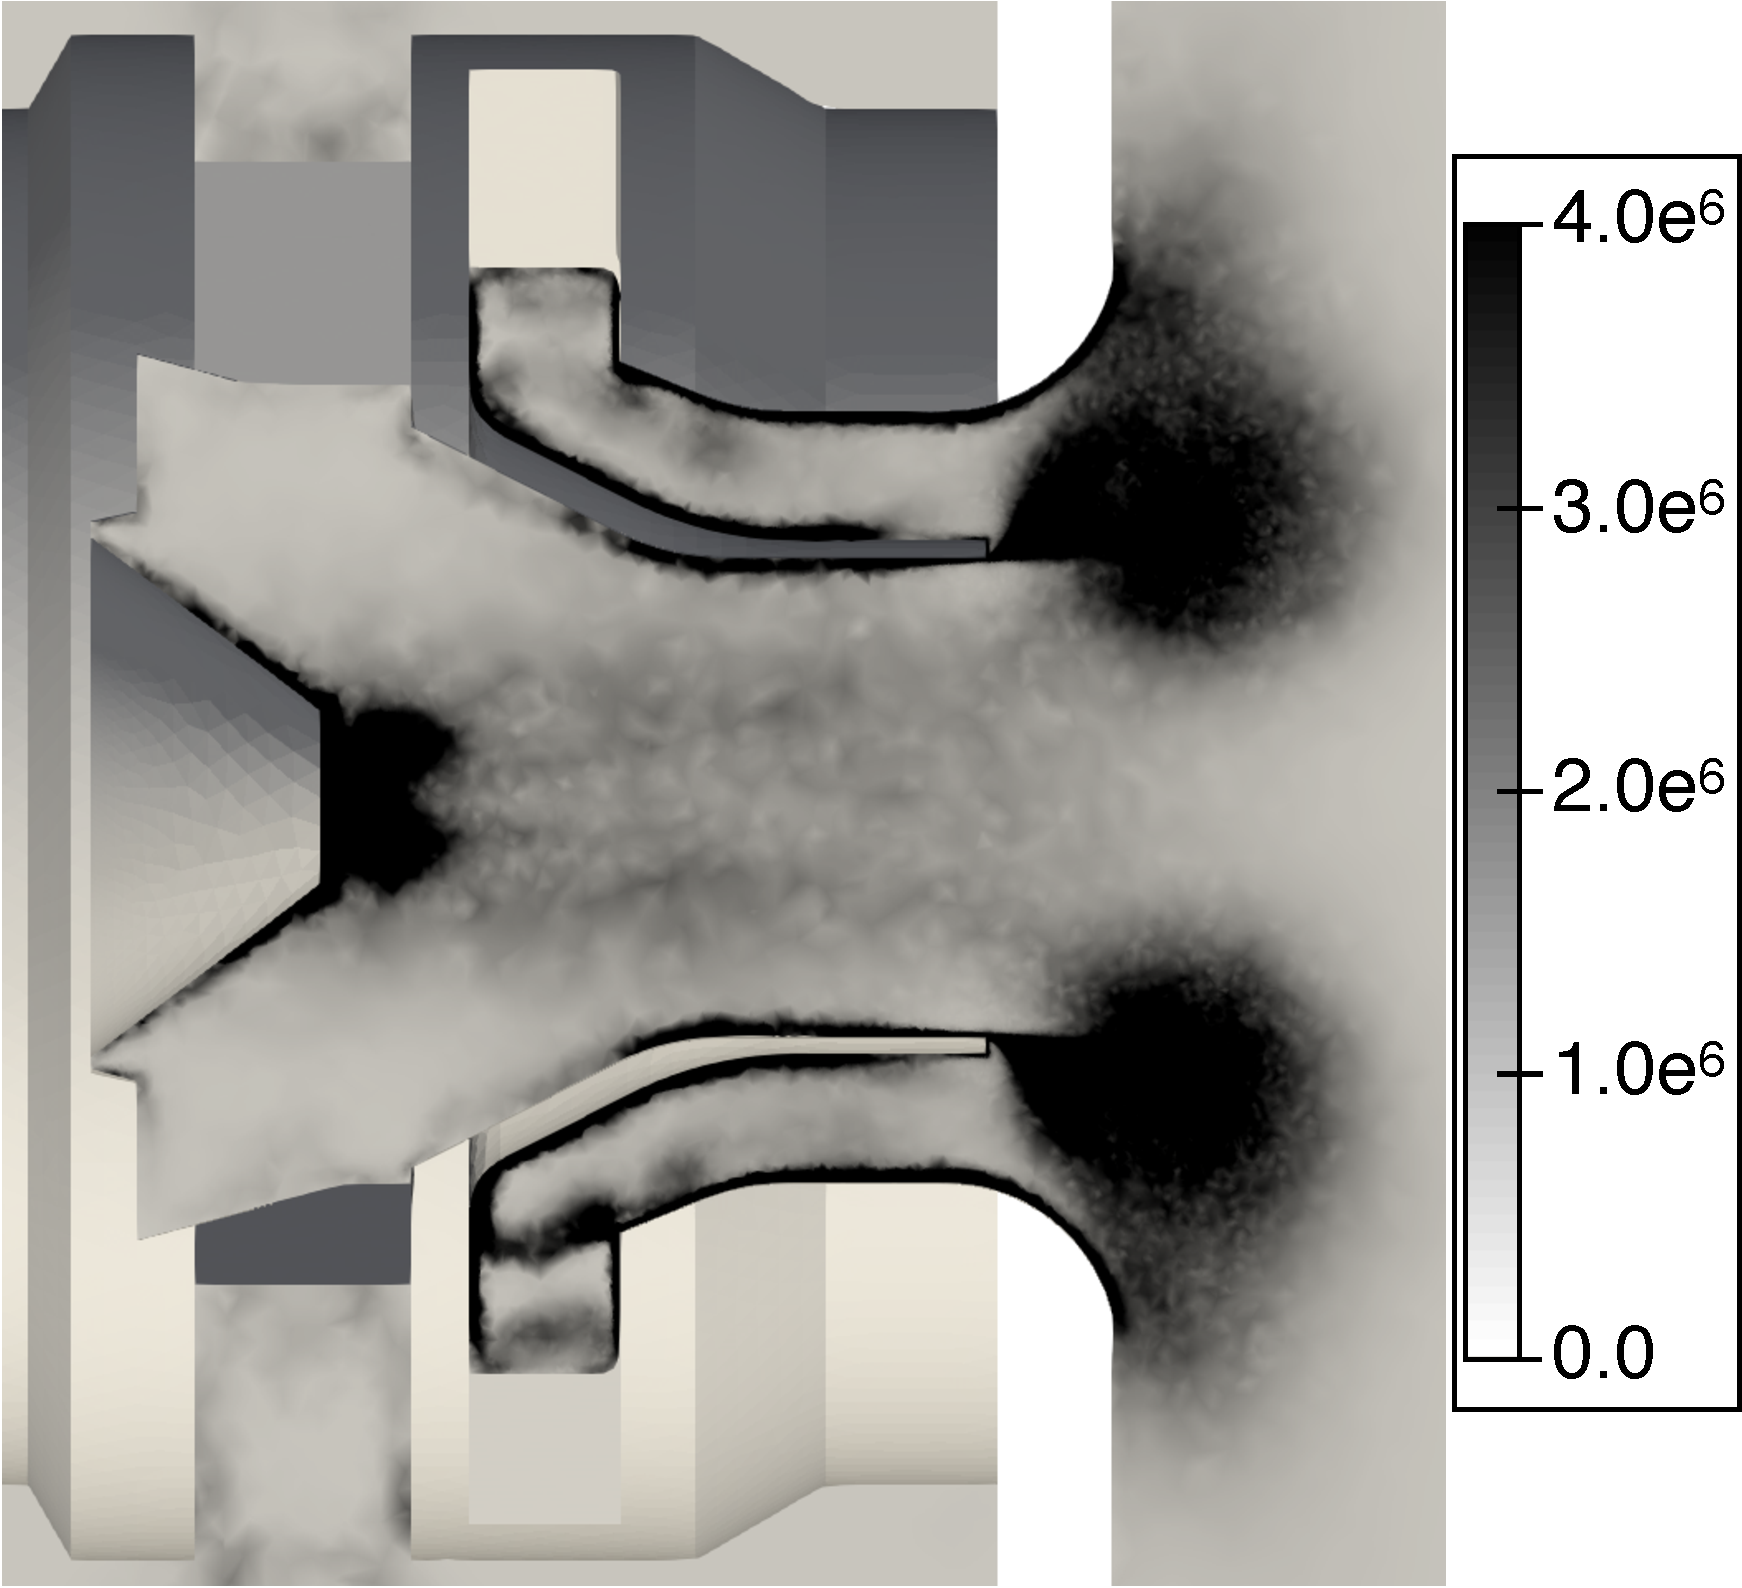
\includegraphics[width = 0.49\textwidth]{fig/applications/swirler/LikeMax}
        }
\caption{Fields of mean kinetic energy dissipation (${W\per\cubicmetre}$) for two geometries with $\sim2$\% channel size difference with the reference case.}
\label{fig:swirler_mod_phi}
\end{figure}

\begin{figure}[!h]
\centering
        \subfloat[$\Delta P \sim \unit{\numprint{4020}}{\pascal}$]{
                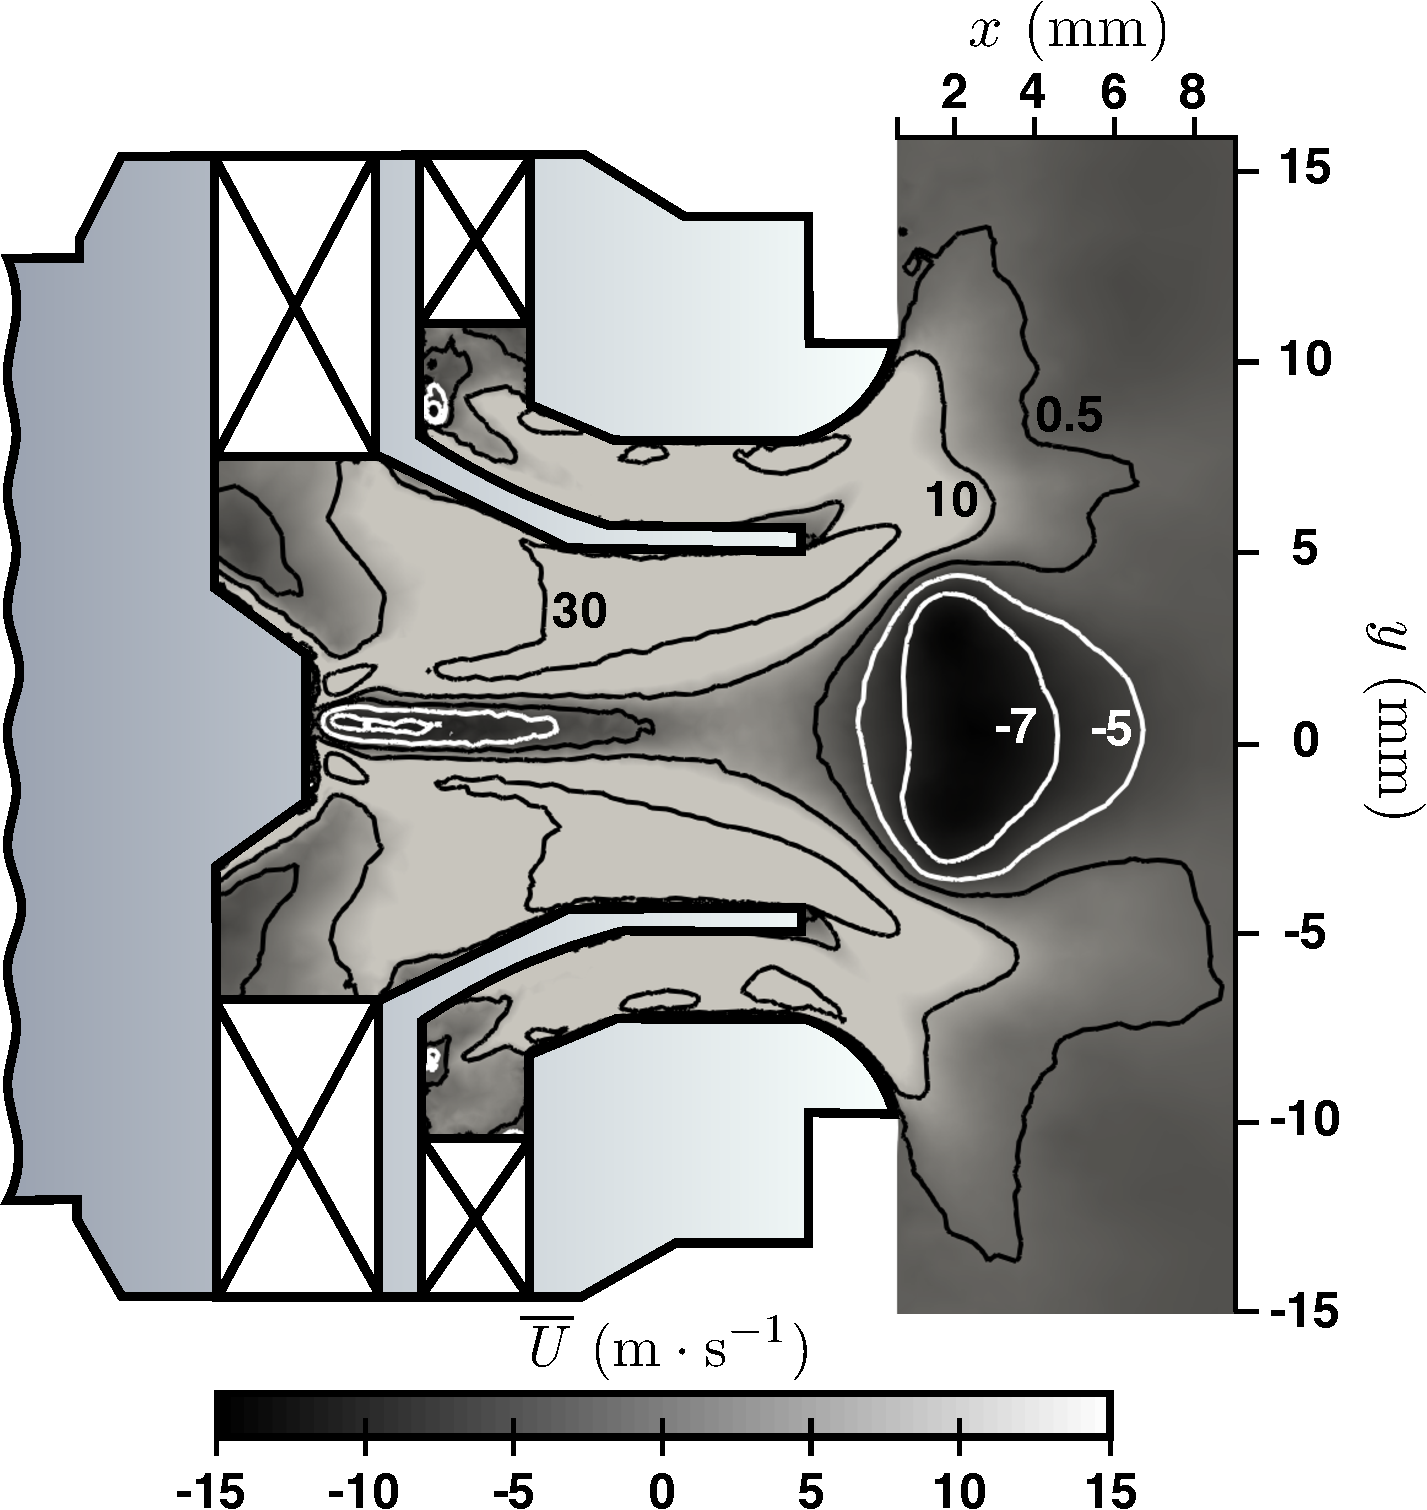
\includegraphics[width = 0.49\textwidth]{fig/applications/swirler/Umin}
        }
        \subfloat[$\Delta P \sim \unit{\numprint{4260}}{\pascal}$]{
                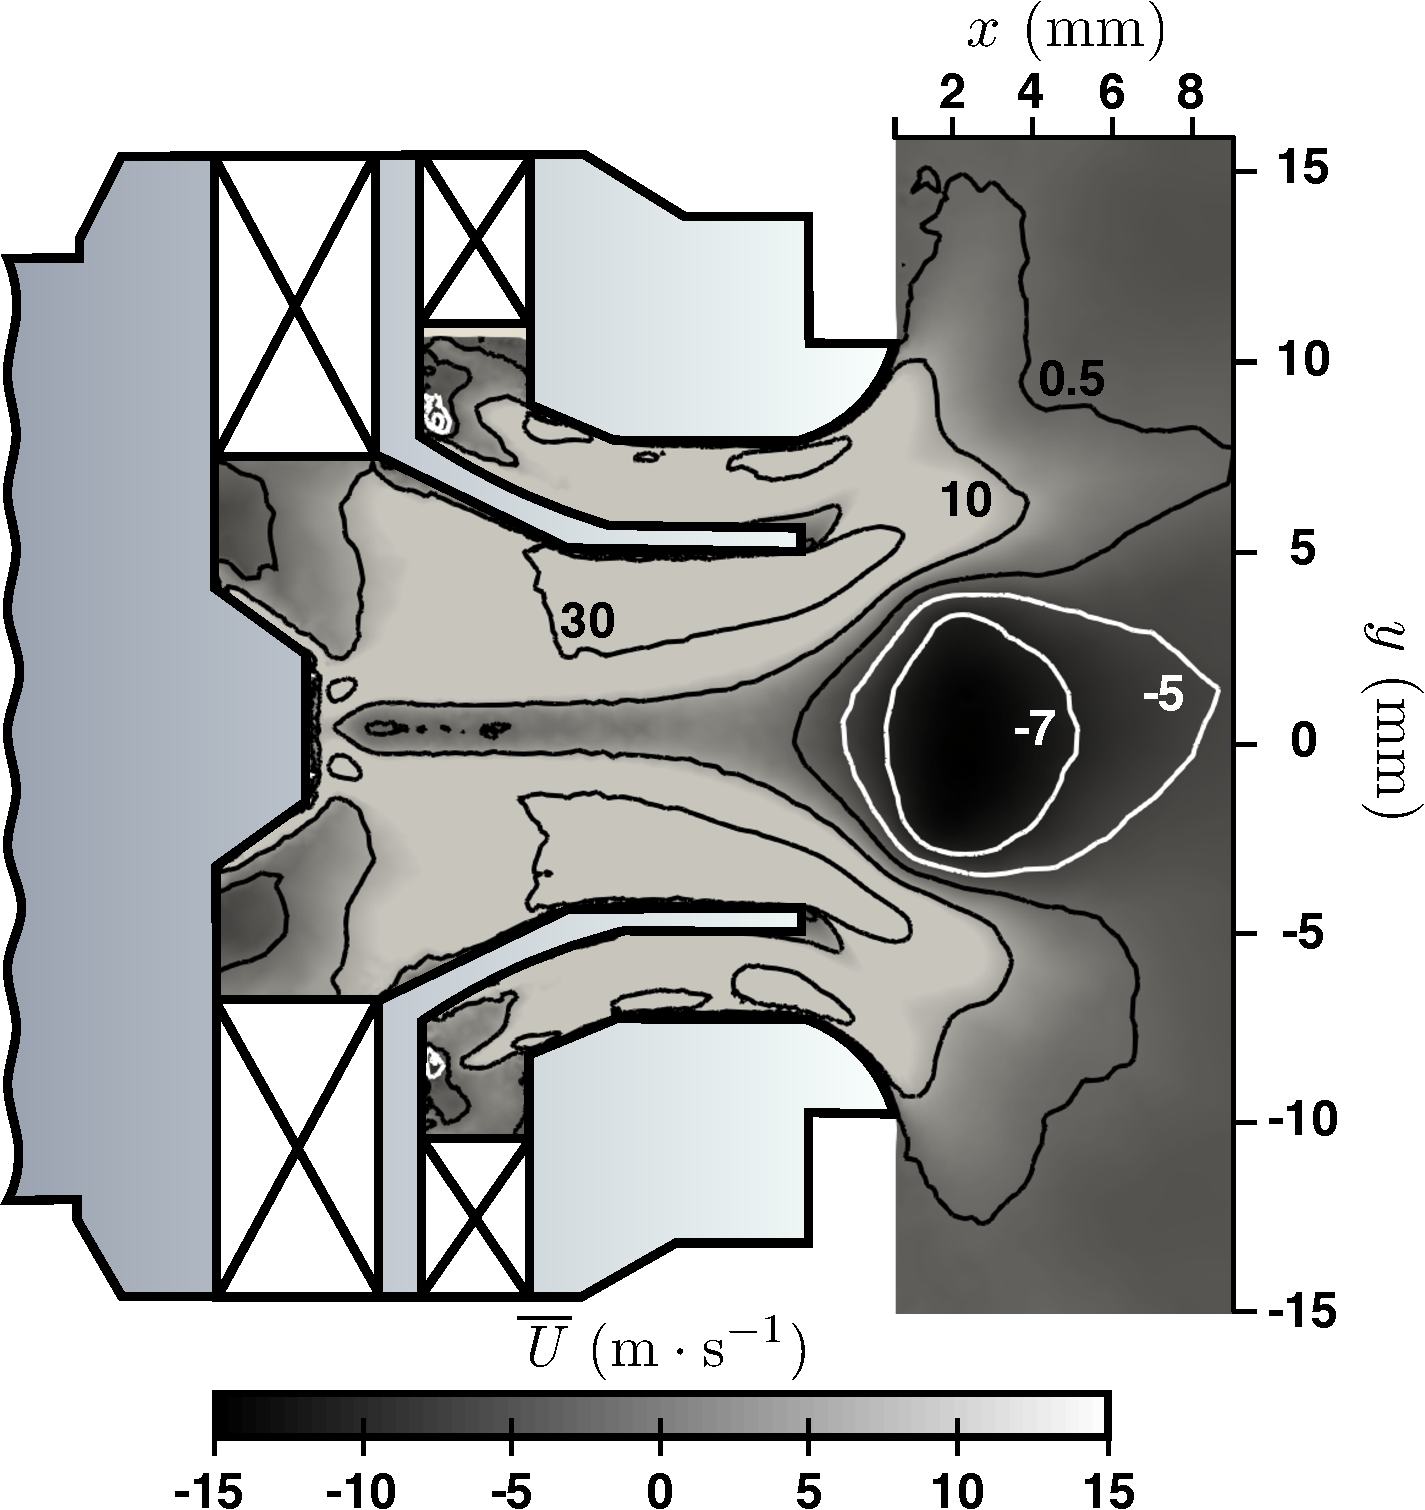
\includegraphics[width = 0.49\textwidth]{fig/applications/swirler/Umax}
        }
\caption{Field of mean axial velocity for two geometries with $\sim2$\% channel size difference with the reference case. \emph{Black} isocontours denote positive velocity, while \emph{white} isocontours denote negative velocity.}
\label{fig:swirler_mod_u}
\end{figure}

\begin{figure}[!h]
\centering
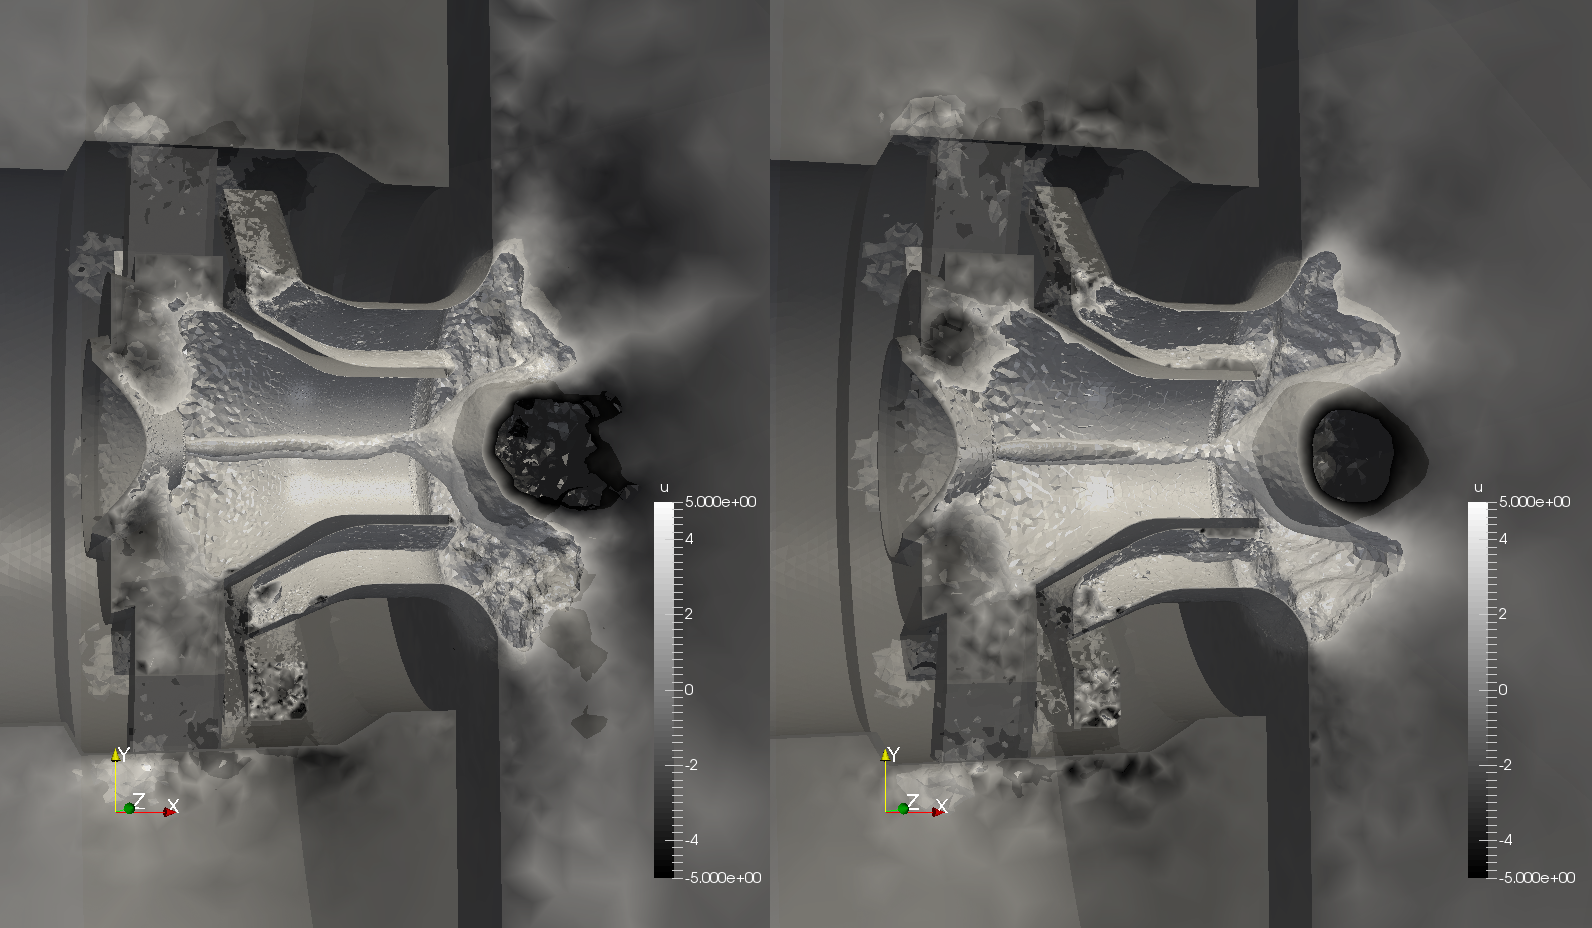
\includegraphics[width=\linewidth,keepaspectratio]{fig/applications/swirler/recirculation_base-mod.png}
\caption{\emph{Q}-criterion colored by mean axial velocity for two geometries with $\sim2$\% channel size difference with the reference case. \emph{Left} $\Delta P \sim \unit{\numprint{4020}}{\pascal}$, \emph{right} $\Delta P \sim \unit{\numprint{4260}}{\pascal}$.}
\label{fig:swirler_mod_u_3d}
\end{figure}

\section{Dimensionality Reduction and Statistical Analysis of Uncertain Parameters}\label{sec:dim}
Performing a UQ study requires a large number of numerical simulations in order to converge statistical moments. If the number of parameters is also large, an even larger number of samples is required. In the present case (\cref{sec:swirler}), the uncertain parameters are the dimensions of all 16 channels. For each channel, this parameter induces a modification of the cross section area. However the channel dimensions, resulting from AM, are not independent and the number of independent parameters can be reduced. Indeed, AM is a layer-by-layer process which precision relies on the ability of the machine to build up and polish these layers. All channels of one stage being built simultaneously, a systematic bias is introduced. 

A set of 5 various real swirler geometries issued from AM was obtained from an engine manufacturer. Thanks to the layering process, two groups of channels are considered to separate the two stages: (\emph{i}) the inner set (first stage) of channels is noted $s=in$, and (\emph{ii}) the outer set (second stage) of channels is noted $s=ou$. Data of each of these two groups is aggregated in the form of a function: $d_{s}(i)$ with $d$ the channel dimension, $i$ the channel number and the subscript $s$ standing for the inner or the outer set. 

The dataset is then represented as a matrix, each line containing the curve $d_{s}(i)$ corresponding to each channel geometry. In order to reveal the correlations in the data and reduce the number of parameters for the UQ study, this matrix is decomposed using a Principal Component Analysis (PCA)~\cite{AnindyaChatterjee2000}, which allows to represent data with a finite number of modes. This compression process turns the functional representation into a scalar representation in a reduced space. The retained variance from the initial data increases with the number of modes of the PCA. In this work, more than 90\% of the original dataset variance is retained with only three PCA components per stage, as shown in~\cref{fig:variance}. The 16 independent uncertain parameters are then reduced to 6 independent parameters (three for each stage), while still accounting for 90\% of the total variance of the original dataset. 

\begin{figure}[!h]
\centering
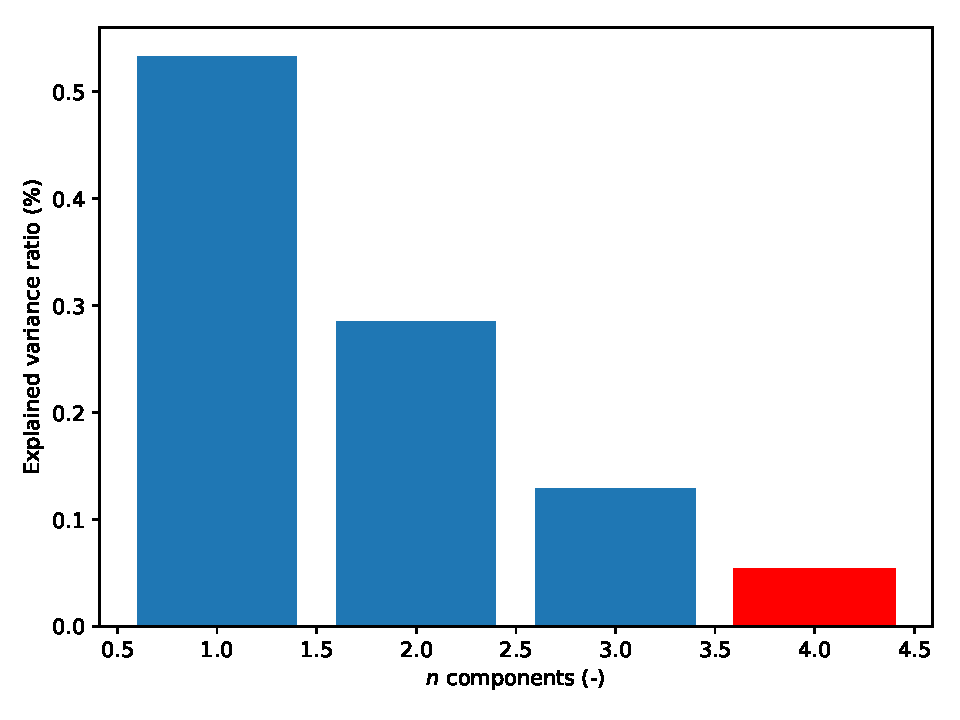
\includegraphics[width=0.7\linewidth,height=\textheight,keepaspectratio]{fig/applications/swirler/variance_ratio.pdf}
\caption{Contribution to the explained variance of the first four modes for the outer channels (similar results for inner channels are not shown). Summing the first three modes only (in blue) and ignoring the fourth mode (in red) corresponds to more than 90~\% of the variance of the original dataset.}
\label{fig:variance}
\end{figure}

Within the reduced space of PCA components noted $\mathbf{x_r}$, the Highest Density Region (HDR) boxplot method~\cite{Hyndman2009} is used to summarize the data statistics and infer new swirler geometries. To determine the HDR, the PDF $f(\mathbf{x_r})$ is built with a multivariate KDE (see~\cref{sec:up}). From this PDF estimator, the HDR reads:
\begin{align}
R_\alpha = \left\{ \mathbf{x_r}: \hat{f}(\mathbf{x_r}) \geq f_{\alpha} \right\}
\end{align}
\noindent with $f_{\alpha}$ such that $\int_{R_\alpha} \hat{f}(\mathbf{x_r}) d x_r = 1 - \alpha$. With this definition, the HDR corresponds to the region of highest PDF with a cumulative probability of $1-\alpha$. The 50\% and 90\% HDR are computed, corresponding respectively to $\alpha=0.5$ and $\alpha=0.1$. By construction  a HDR develops around the maximum PDF $\max \{\hat{f}(\mathbf{x_r})\}$ which identifies the most probable mode. Transposed using the inverse transform from the reduced space to the original space, this most probable mode corresponds to the "central curve"---also referred to as the median curve. To summarize, in the original space the median curve corresponds to the most probable set of values that defines a swirler geometry manufactured with AM, while the 50\% and 90\% HDR express the data dispersion.

The PDF estimator and the HDR allow to infer new realizations that are statistically relevant to the original dataset and can be used for the UQ analysis. This is done in the next section. 

\section{Generation of datasets }\label{sec:res}

In the 3 PCA-components space defined from the experimental database, a set of 30 points was sampled from a low discrepancy sequence of \emph{Sobol'} (scrambled)~\cite{Cavazzuti2013,Kucherenko2015} which ensures a good coverage of low-dimensional parameter spaces. The 30 points are plotted in \Cref{fig:samples-scatter}~in 2D cuts of the 3D parameter space of each swirler stage. The PDF estimators obtained for each PCA component are shown in the plots placed along the diagonal of the figure.  

\begin{figure*}[!h]
\centering
\subfloat[Inner channels]{
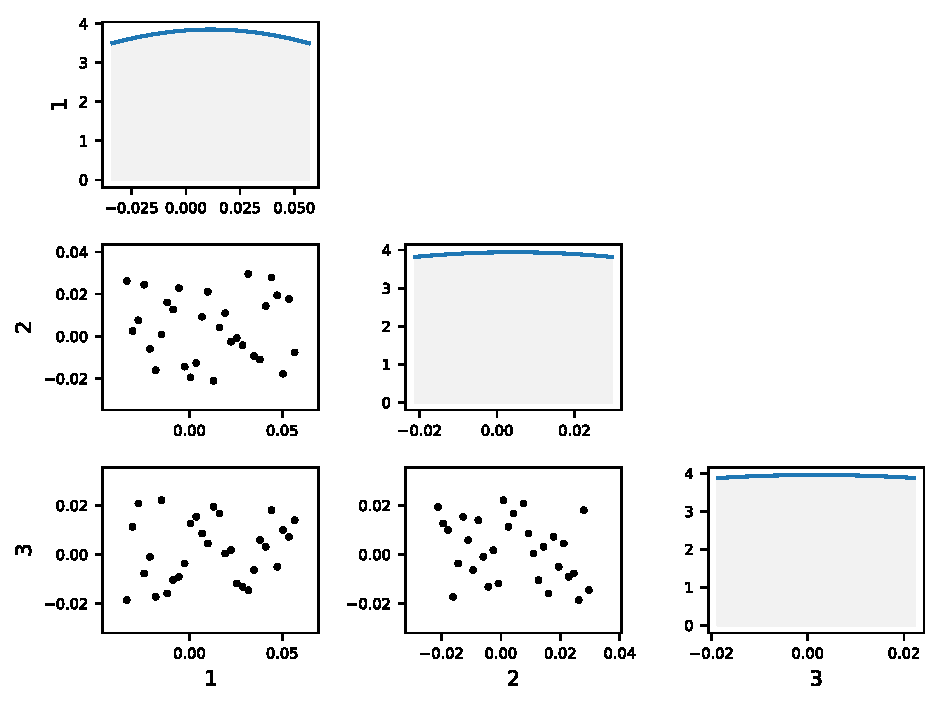
\includegraphics[width=0.49\textwidth,height=\textheight,keepaspectratio]{fig/applications/swirler/inner_samples_scatter.pdf}
}
\subfloat[Outer channels]{
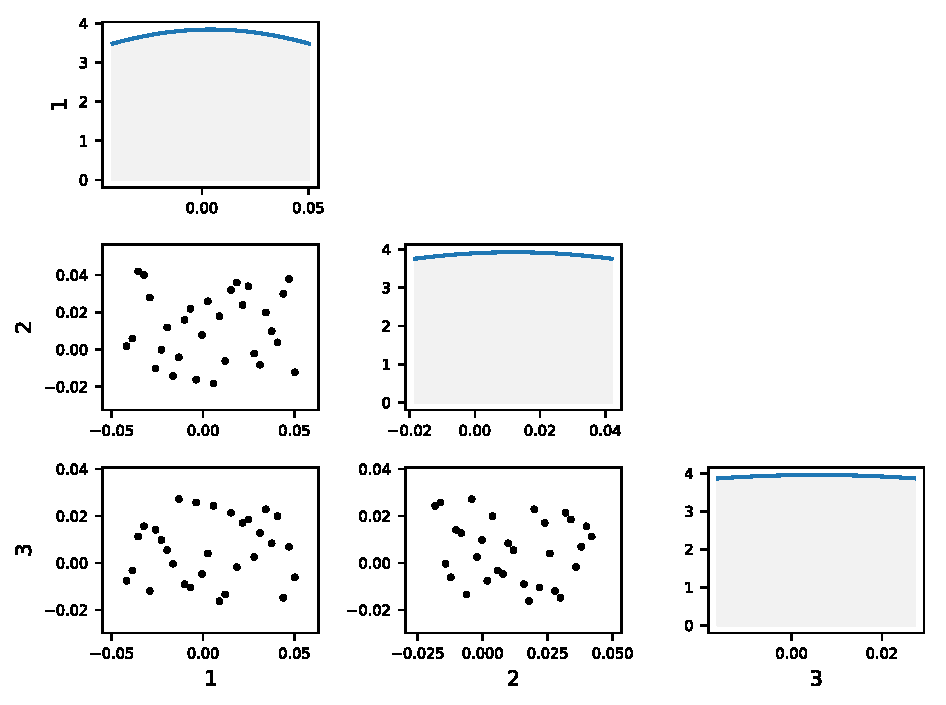
\includegraphics[width=0.49\textwidth,height=\textheight,keepaspectratio]{fig/applications/swirler/outer_samples_scatter.pdf}
}
\caption{Bivariate principal component score plots of the 30 generated samples in the reduced PCA parameter spaces of the inner and outer stages. Each point corresponds to a curve sample. Probability distributions for each component are shown in the diagonal plots: \emph{lines} represent the kernel PDF estimator and \emph{Shaded} areas are histograms (from which are based the scaling of the \emph{y-axis}).}
\label{fig:samples-scatter}
\end{figure*}

\begin{figure*}[!h]
\centering
\subfloat[Inner channels: $d_{in}(i)$]{
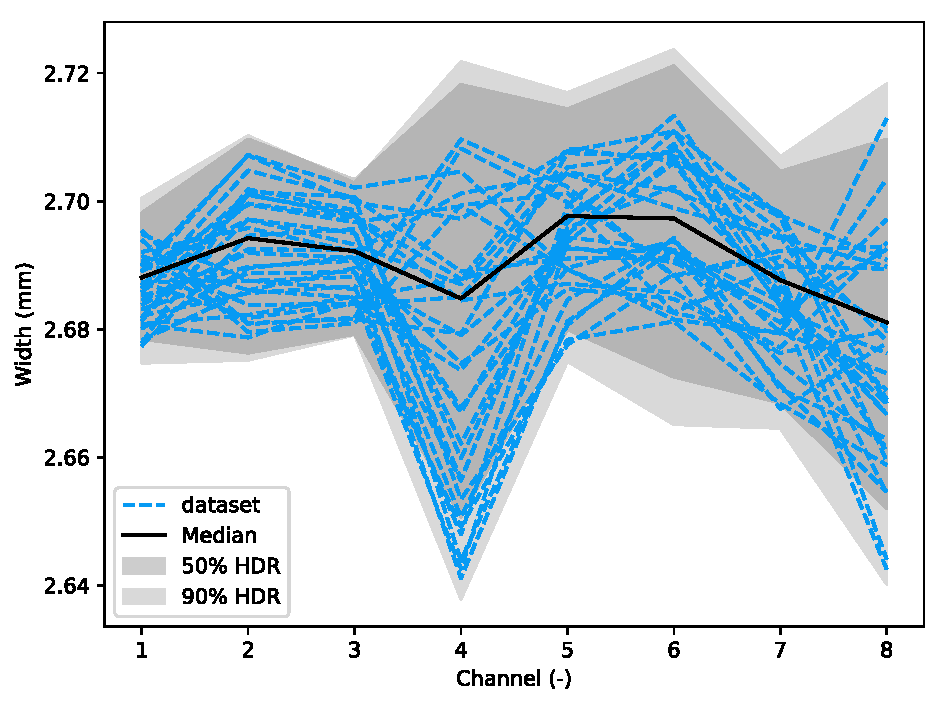
\includegraphics[width=0.49\textwidth,height=\textheight,keepaspectratio]{fig/applications/swirler/inner_samples.pdf}
}
\subfloat[Outer channels: $d_{ou}(i)$]{
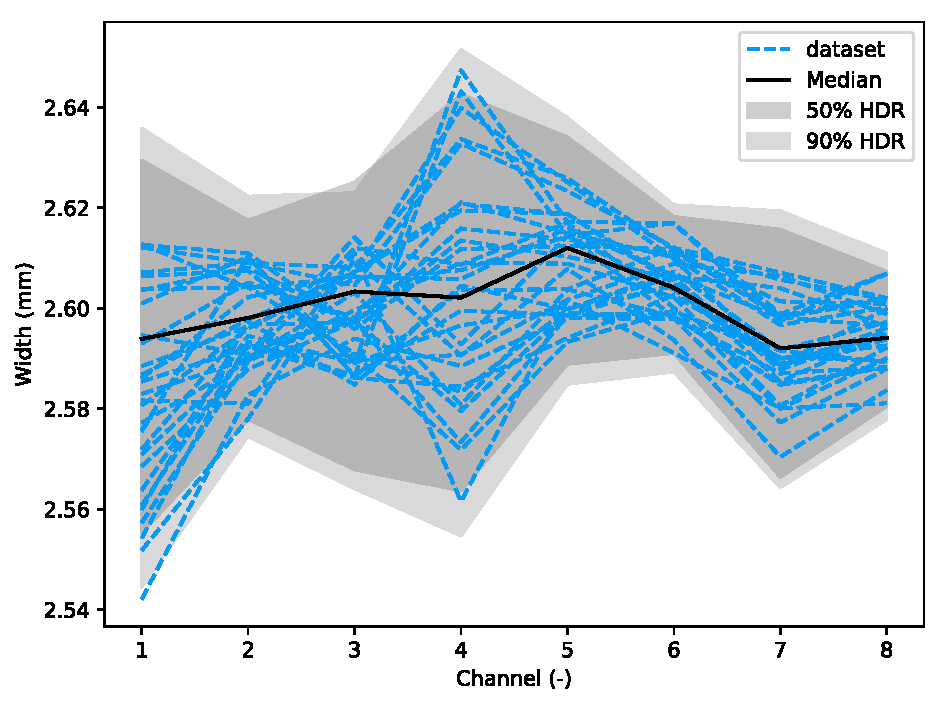
\includegraphics[width=0.49\textwidth,height=\textheight,keepaspectratio]{fig/applications/swirler/outer_samples.pdf}
}
\caption{Statistics of channel dimensions: median curve (\emph{bold solid} line) and 50\% and 90\% HDR (\emph{shaded} areas). Blue \emph{dashed} lines represent the 30 generated samples.}
\label{fig:samples}
\end{figure*}

\Cref{fig:samples}~shows the 30 curves in the initial parameter space (channel dimensions) corresponding to the inverse transform of the 30 generated datasets. It can be noted that 30 curves are well distributed around the median line, inside the 90\% HDR, confirming that the sampling is statistically relevant to the original dataset. Thus this method is able to reproduce statistically relevant scenarios of swirler geometries.

The number of samples was chosen to minimize the computational time (see ~\cref{sec:swirler}). From~\cite{Forrester2007}, it should be at least $10 n_{dim}$, with $n_{dim}$ the number of parameters, leading in our case to 60 samples. However, as we are interested in small variations in the parameter space the variation of the quantity of interest (pressure loss) is not expected to require as many samples and it can be said with confidence that 30 simulations are enough to describe it.

A larger initial database could reveal even more correlations between the parameters, allowing to further reduce the number of parameters. With the 5 datasets used here, a large dispersion of the different realizations is observed in~\cref{fig:samples} and there is no room for more reduction. Still, it is clear that the 16 initial  parameters of the 5 datasets are not independent, which is essential for the current study as keeping all 16 parameters independently would have required an enormous number of simulations.

\section{Results and Discussion}\label{sec:disc}

\begin{figure}[!ht]
\centering
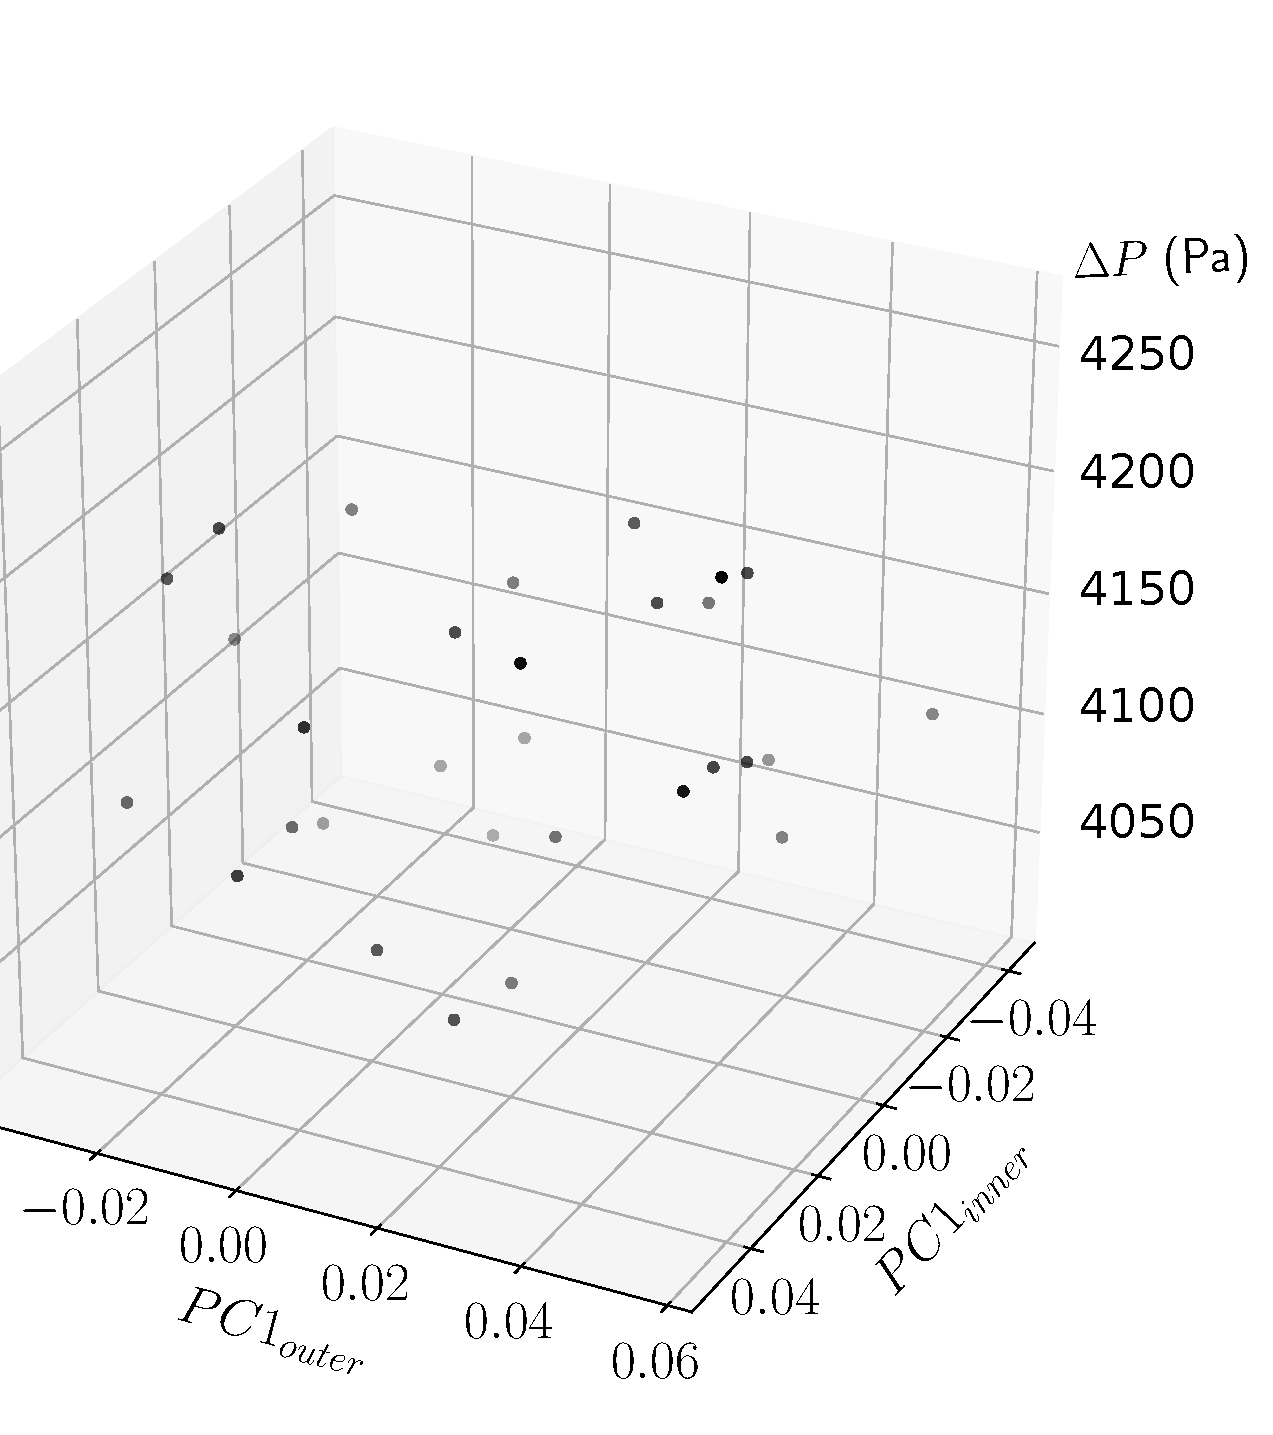
\includegraphics[width=0.6\linewidth,keepaspectratio]{fig/applications/swirler/scatter_3D.pdf}
\caption{Pressure loss function of the first components of the reduced space.}
\label{fig:scatter-dp}
\end{figure}

\Cref{fig:scatter-dp} shows the evolution of the pressure loss by varying the channel dimensions. As the design of experiments consists of 6 parameters, the response is presented in a 2-dimensional plot where the first modes of both inner and outer channels are used. Indeed the fitst modes contribute the most to the variance of the data. In \cref{fig:scatter-dp} no cluster of points appears at any particular level of pressure drop and the pressure loss distribution is relatively uniform among the samples. Summary statistics are presented in~\cref{tab:summary-stats} and the probability distribution of the ensemble is shown in~\cref{fig:pdf-dp}.  All these results indicate that the response of the system to these geometrical modifications is rather uniform: the geometrical uncertainties are transmitted through the system without amplification.

\begin{table}[!ht]
\centering
\caption{Summary statistics of the pressure drop of the 30 LES.}
\begin{tabular}{lccccc}
\toprule
& Mean & Median & Std & Min & Max\\
\cmidrule{2-6}
Pressure drop (Pa) & 4128 & 4133 & 65 & 4020 & 4260\\
\bottomrule
\end{tabular}
\label{tab:summary-stats}
\end{table}

\begin{figure}[!ht]
\centering
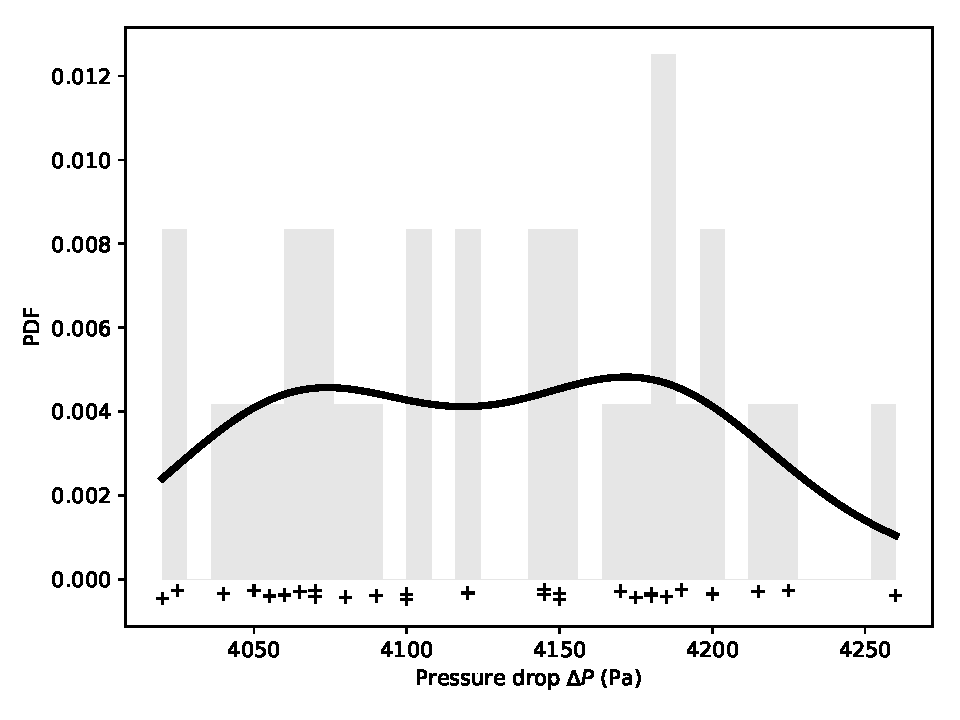
\includegraphics[width=0.6\linewidth,keepaspectratio]{fig/applications/swirler/pdf_dp_ensemble.pdf}
\caption{PDF of the pressure loss over the dataset (\emph{black} line) reconstructed using KDE. \emph{Crosses} represent the samples, and the \emph{shaded} area is a histogram view.}
\label{fig:pdf-dp}
\end{figure}

As a consequence of this uniformity with no clear structure, it is difficult to build a reduced model. Several surrogate model strategies available in BATMAN---see~\cref{sec:swirler}---such as Gaussian process, polynomial chaos and Radial Basis Functions were tested, but none of these methods were able to fit the data and infer a satisfactory result. The reported quality---assessed by Leave-one-out cross validation~\cite{Kohavi1995}---was negative, which implies that the tested surrogate models are worse than a simple constant guess.

To further analyse the results, \cref{fig:dp-surface} shows the variation of the pressure loss with the total channel section area for each simulation. Again no clear pattern is making out. The swirl numbers---definition from Merkle~\cite{Merkle2006}---for cases with maximum, minimum and middle value of pressure drop are summarized in~\cref{tab:swirl}. It is interesting to see that despite pressure drop variation, the swirl number which drives the characteristics of the flow stays within negligible variation close to the theoretical value of $S=0.76$ in all three cases. These observations are confirmed by the comparison of the mean axial velocity profiles downstream the nozzle exit compared with PIV measurement for the same three cases (\cref{fig:profile-u}). Details and discussion about PIV are given in Daviller \textit{et al.}~\cite{Daviller2017}. Very close curves are obtained for the three LES at the shown positions. This means that, in accordance with the unchanged swirl number, no significant change occurs in the flow field downstream the nozzle. This is confirmed by the PSD of mean axial velocity at the plug tip in~\cref{fig:psd-u}. Each simulation exhibit a $k^{-5/3}$ slope over a range of frequency $5\time10^3 \leq f (Hz) \leq 5\time10^4$, characteristic of the inertial range of turbulent flows.

All in all, it ensures that the flame will be stable even though there is a change in pressure loss.


\begin{table}[!ht]
\centering
\caption{Swirl numbers for three different geometries.}
\begin{tabular}{lccc}
\toprule
& $\Delta P_{middle} =\unit{\numprint{4145}}{\pascal}$& $\Delta P_{min} =\unit{\numprint{4020}}{\pascal}$& $\Delta P_{max} = \unit{\numprint{4260}}{\pascal}$\\
\cmidrule{2-4}
Swirl number & 0.7609 & 0.7582 & 0.7639\\
\bottomrule
\end{tabular}
\label{tab:swirl}
\end{table}

\begin{figure}[!ht]
\centering
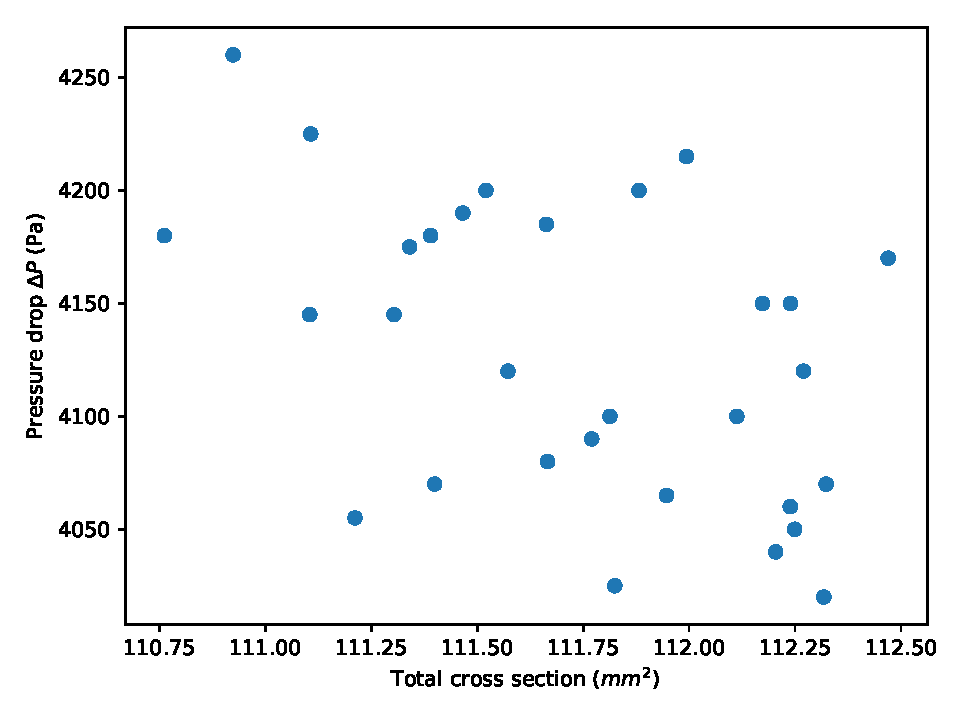
\includegraphics[width=0.6\linewidth,keepaspectratio]{fig/applications/swirler/dp_surface.pdf}
\caption{Pressure drop as a function of the total cross section channel area. Each point represents a sample.}
\label{fig:dp-surface}
\end{figure}

\begin{figure*}[!ht]
\centering
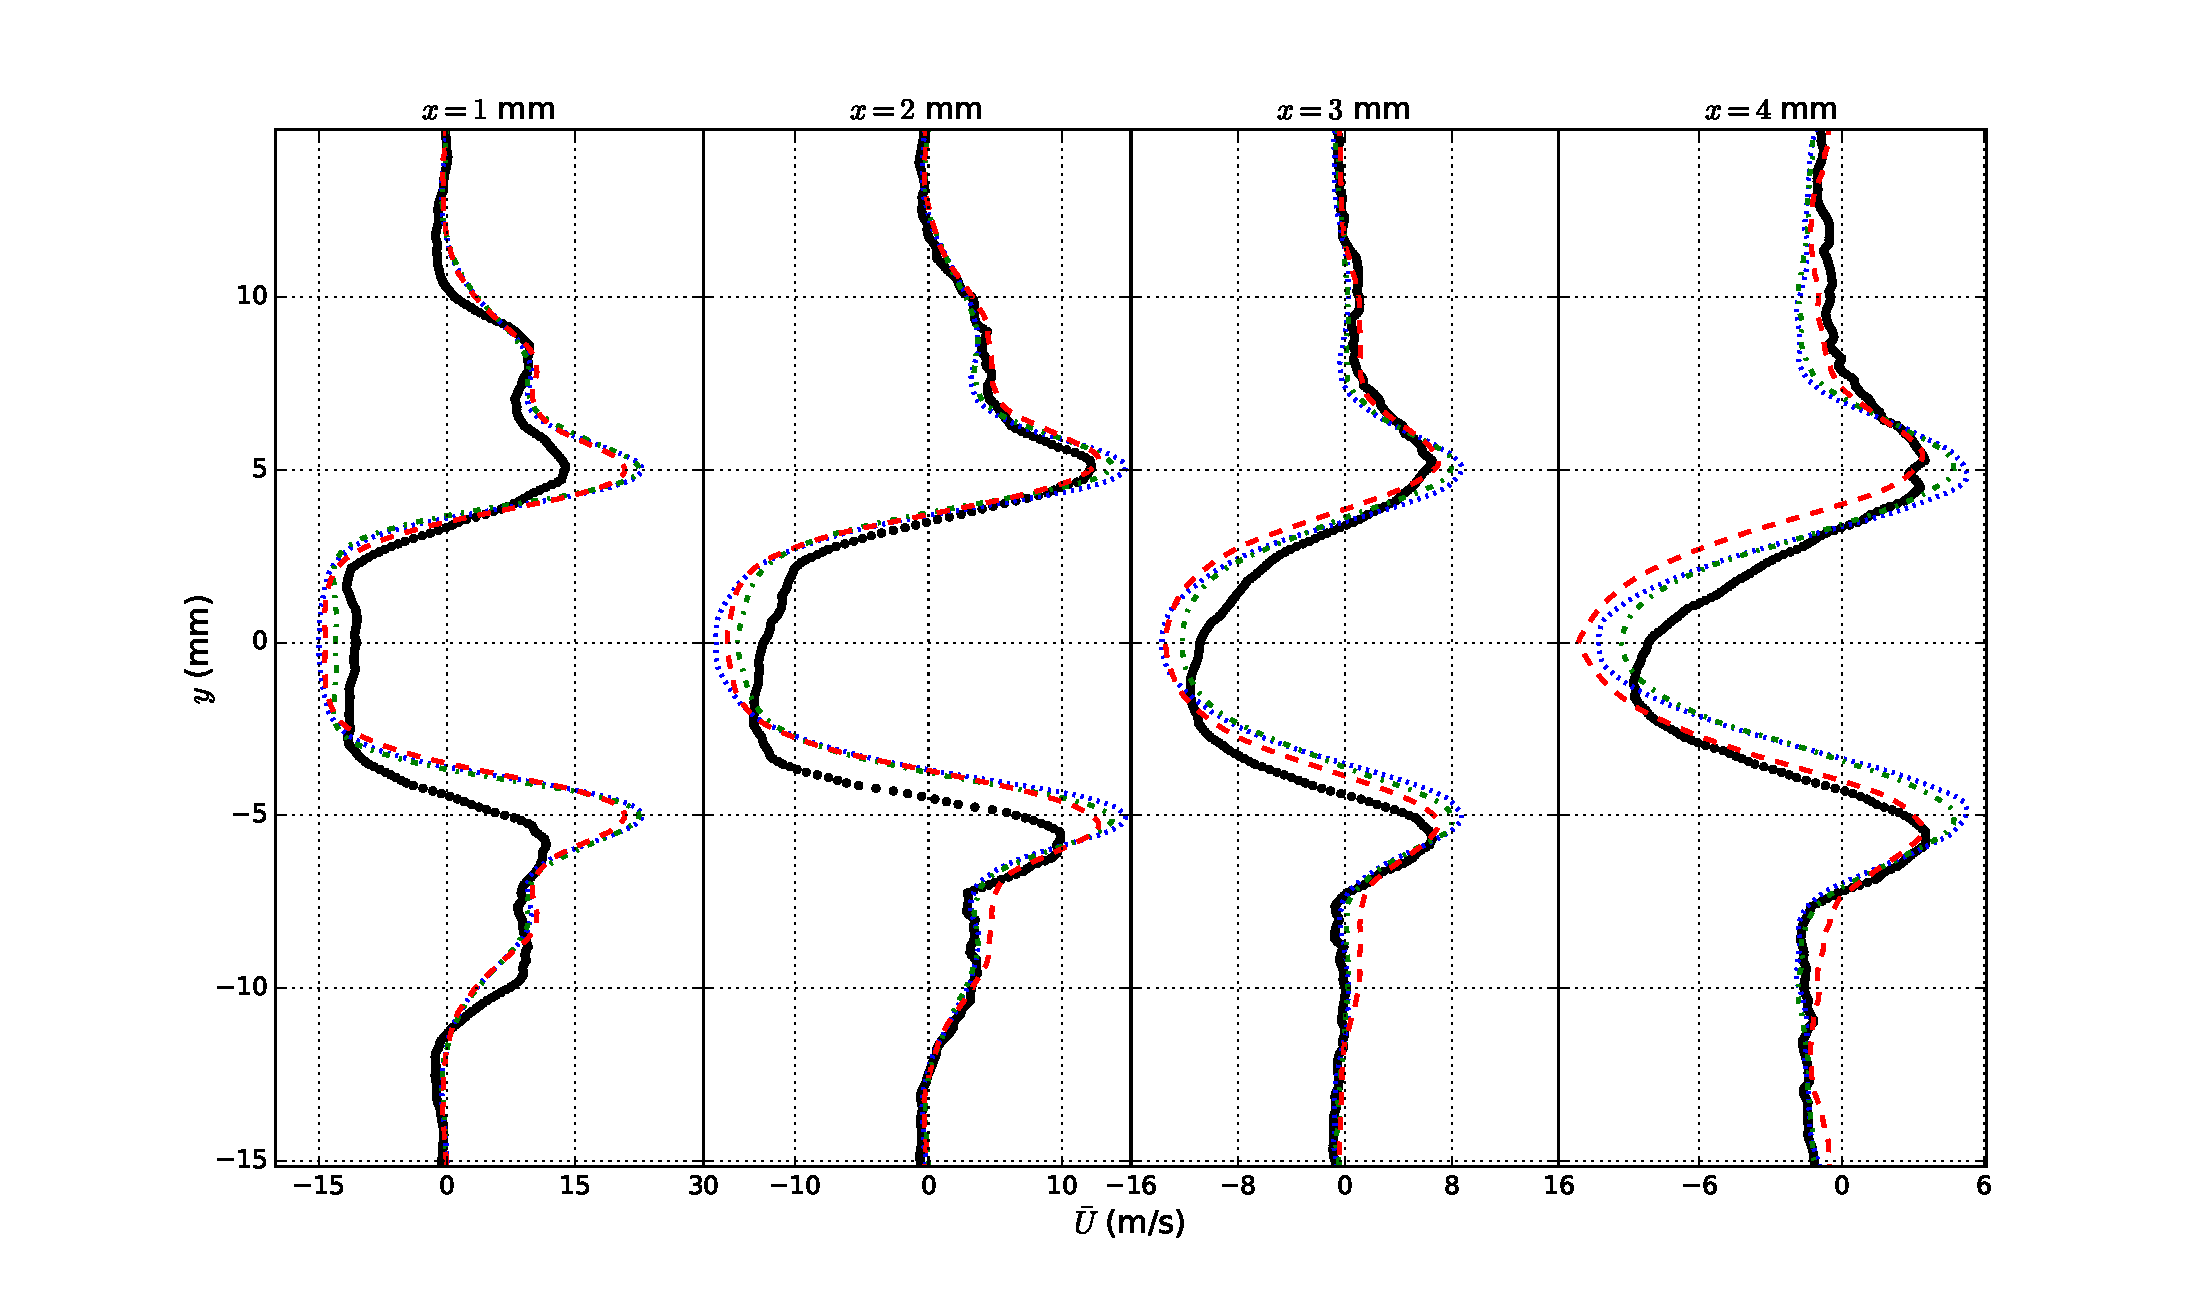
\includegraphics[width=\linewidth,keepaspectratio]{fig/applications/swirler/profile_u.pdf}
\caption{Mean axial velocity profiles at four axial locations (from left to right $x = \unit{1, 2, 3, 4}{\milli\metre}$) obtained with LES and in the experimental setup (black \emph{circles}). \emph{Dotted lines} $\Delta P_{middle} =\unit{\numprint{4145}}{\pascal} $, \emph{dashed-dotted lines}$\Delta P_{min} =\unit{\numprint{4020}}{\pascal} $, \emph{dashed lines} $\Delta P_{max} = \unit{\numprint{4260}}{\pascal}$.}
\label{fig:profile-u}
\end{figure*}

% PSD
\begin{figure*}[!ht]
\centering
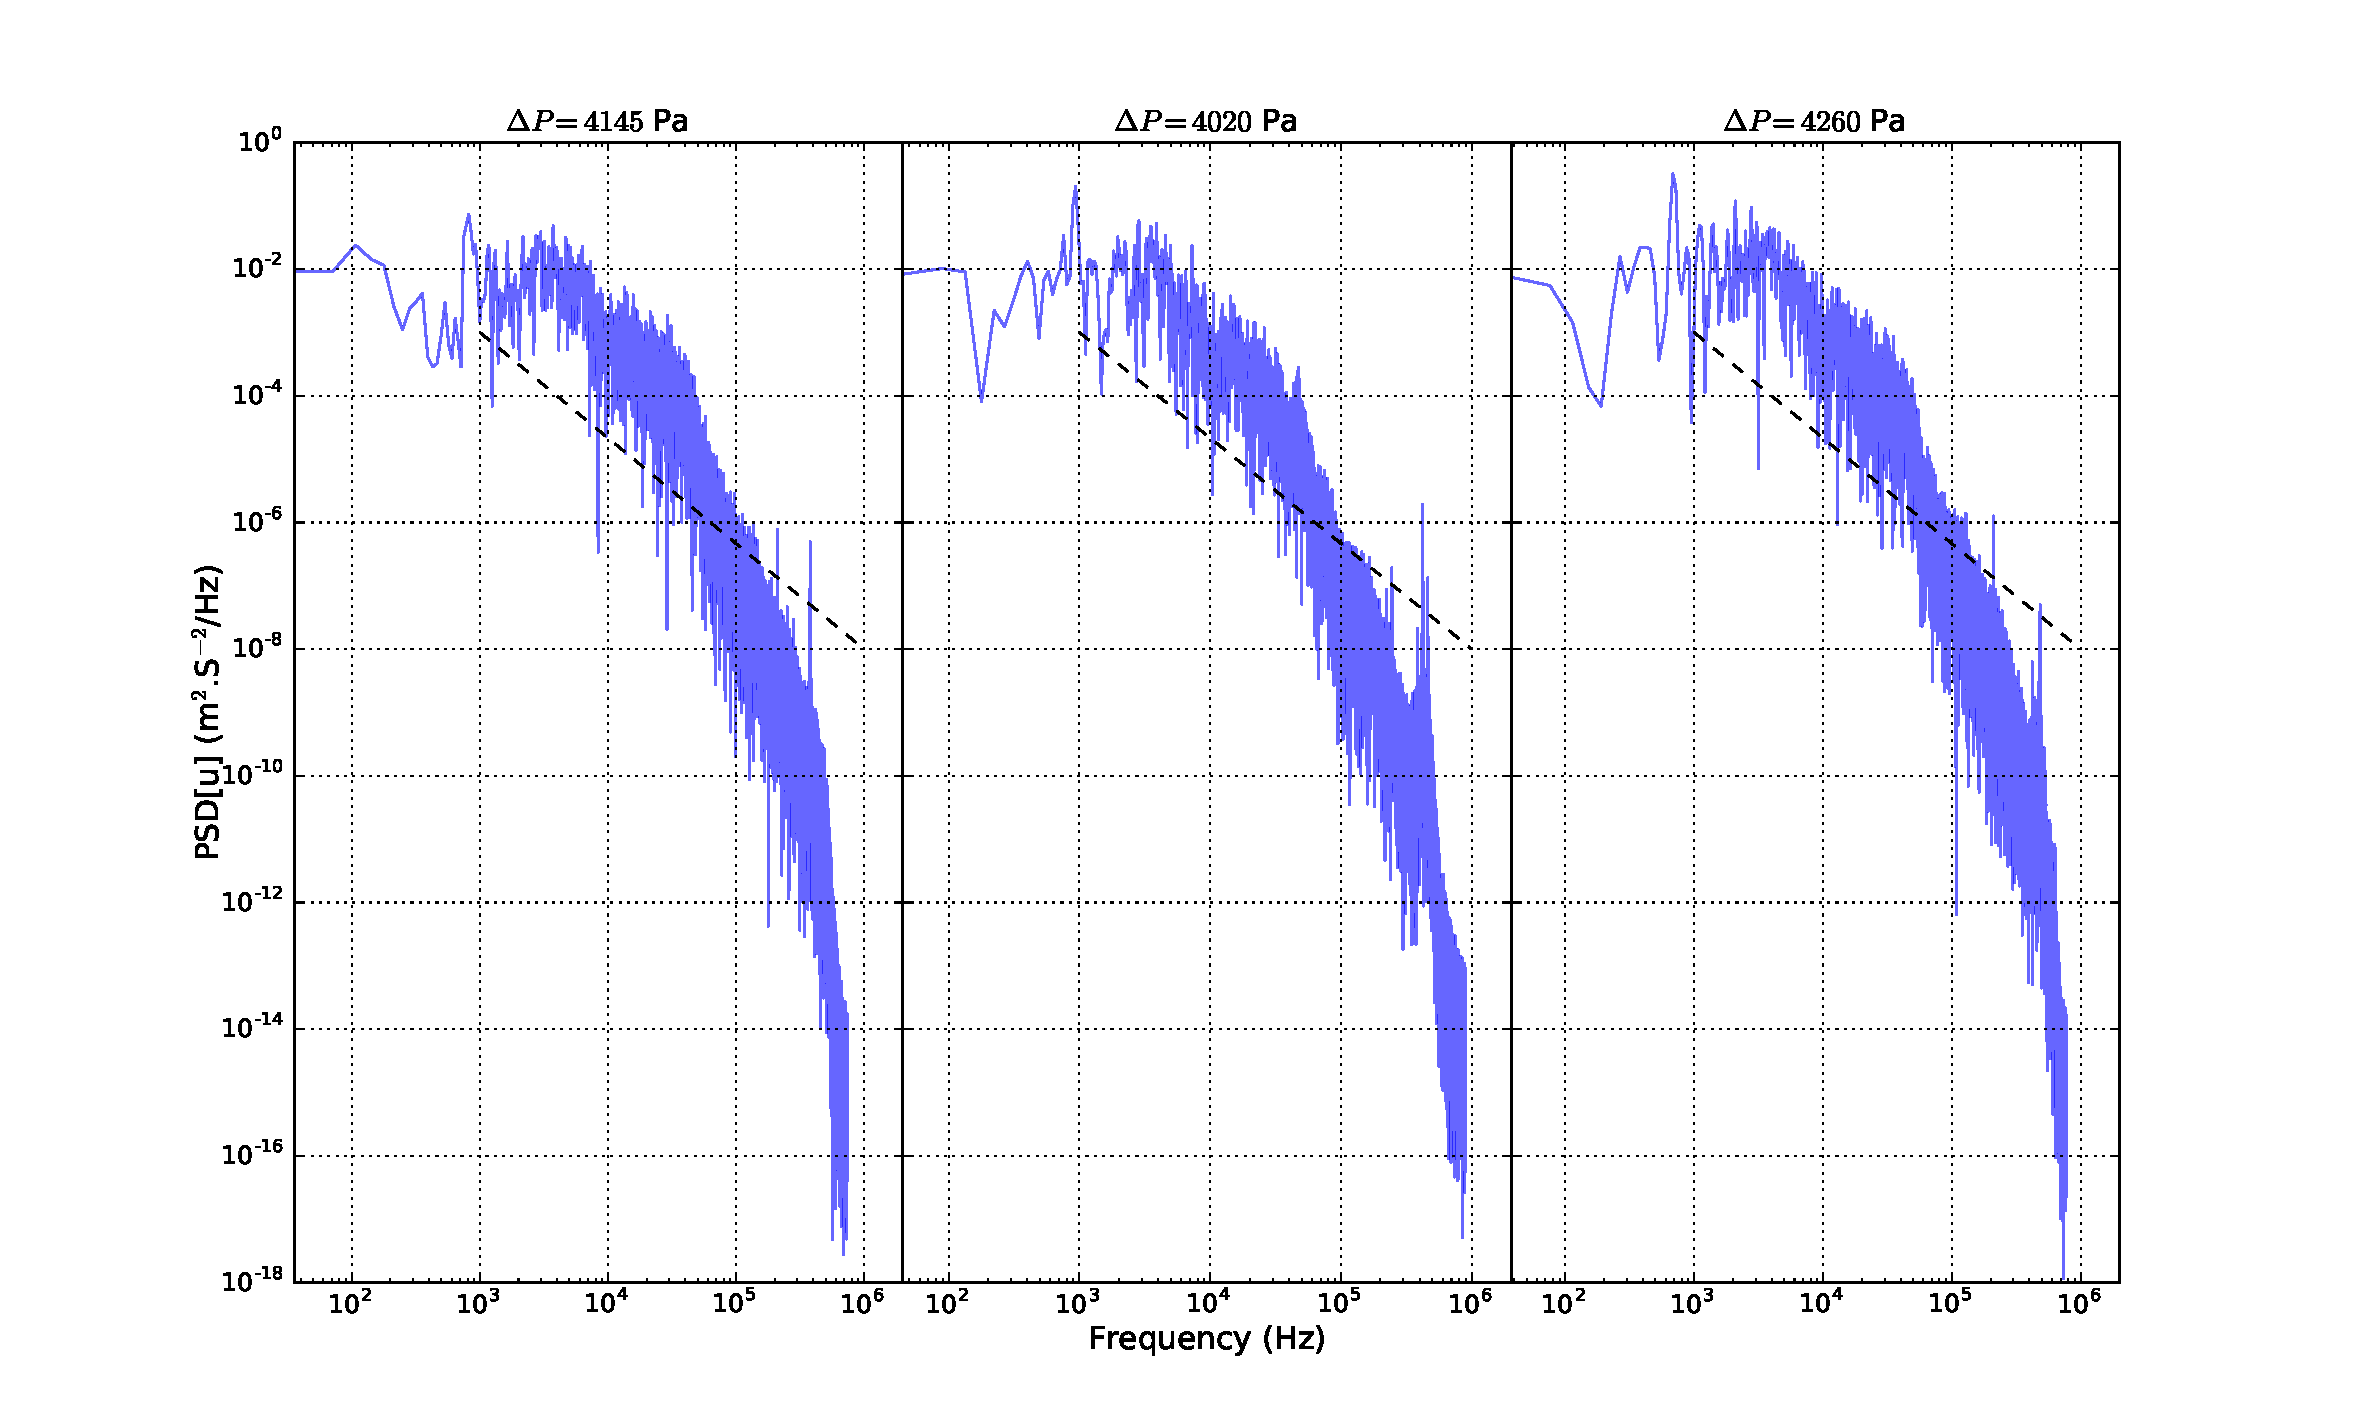
\includegraphics[width=\linewidth,keepaspectratio]{fig/applications/swirler/psd_u.pdf}
\caption{Power spectral density of axial velocity fluctuations for three different geometries at the plug tip.}
\label{fig:psd-u}
\end{figure*}


Although the construction of a surrogate model is not feasible in this case, the present uncertainty analysis highlights the intrinsic and chaotic variability of a self-compensation mechanism in the generated statistical data. This can be explained by: (\emph{i}) the nature of the geometrical modifications, where some channels are widened while others are tightened, limiting the overall impact on the pressure loss; and (\emph{ii}) the amplitude of these modifications which is very small compared to the width of the channels. Indeed, manufacturing defects were limited to a maximum 2\% of the cross section area of a channel, consistently with real observation of AM. Note that in such situation, the ability of the solver to respond with the correctly adapted physics is paramount. To check this, the relative numerical error on the pressure drop was estimated and found less than $1\%$ which is sufficient to capture with accuracy the pressure drop induced variation by geometrical modification of the order of $\simeq 5\%$. Thus, the solver accuracy is sufficient and the results are considered reliable.

\section{Conclusion}
The purpose of this work was to perform an Uncertainty Quantification (UQ) study of a swirler geometry. More precisely, this study focused on geometry deviations due to Additive Manufacturing (AM) and their effects on the pressure loss. As the number of parameters required to characterize the configuration was high, a Principal Component Analysis (PCA) was used, allowing to cut down the number of parameters from 16 to 6 independent variables. Statistic analysis based on Highest Density Region (HDR) highlighted the non-independence of the geometrical parameters and thus the impact of AM. Thanks to a mesh adaptation strategy, a set of 30 different statistically representative cases was accurately simulated with Large Eddy Simulations (LES). The uncertainty analysis then led to an overall view of the variation of the pressure drop induced by geometry changes. Results show that slight discrepancies in the swirler channel dimensions lead to slight differences in the pressure loss, without amplification or damping. This conclusion also holds for the flow, as shown by the comparison of the swirl numbers and velocity profiles. This is a critical information for engine manufacturers, as it means that AM will not affect the flow exiting the swirler and the stability of the flame developing downstream.

The analysis of the intrinsic variability of the system did not exhibit any noticeable pattern. As a consequence, no surrogate model could be built. This is explained by the nature of the modifications and most importantly by their amplitude. Augmenting the range of variability in the system, exploring for example other designs, would increase the impact on the pressure loss. %For the same reason, increasing the mass flow rate may have a stronger effect. Here the mass flow rate was taken as in the experiment~\cite{Daviller2017}, where it was restricted to low values. 

The UQ method used in this work, combining data reduction and high-fidelity LES, paves the way for systematic uncertainty studies in the design phase of industrial systems to take into account manufacturing defects. This may lead to the determination of optimized manufacturing tolerances, and finally to significant cost saving.

\chapter{Optimization of Helically Roughened Heat Exchanger}

\section{Introduction}

% Industrial context
Artificially increasing the roughness of heat exchanger inner surfaces is a passive and efficient method to improve the heat transfer efficiency, which has led to numerous internal designs. The choice of a specific roughness design depends on the flow regime, the fluid properties and might depend on the device application. This method however always induces an increase in pressure loss which is detrimental to the heat exchanger global efficiency and needs to be limited.\\

In this context, numerous experimental studies have investigated various turbulence promoter geometries, such as transverse ribs \cite{webb1971, aliaga1994} or helical ribs \cite{gee1980, VicenteGarciaViedma2004, cheng2006, Mayo2016}. More complex three-dimensional geometries were also investigated such as dimpled tubes \cite{VicenteGarciaViedma2002}. Garcia et al. \cite{GarciaSolanoVicenteEtAl2012} compared the behaviour of corrugated tubes, dimpled tubes and wire coils, concluding to a larger impact of the internal geometry on the pressure drop than on the heat transfer. They also highlighted that better efficiencies are reached with helically corrugated tubes and dimpled coils for Reynolds number greater than 2000, which are geometries comparable to helically continuous and discontinuous ribbed tubes respectively. This result motivates further investigation on the optimal discontinuous helical rib shape in the current work. Based on those studies, empirical correlations for the prediction of friction and heat transfer efficiency in roughened heat exchangers can be found in the literature. In particular, correlations for simple, 2D roughness geometries such as transverse ribs or helical ribs predict quite accurately the heat exchanger efficiencies in a specific range of operating conditions and fluid properties thanks to numerous experimental investigations. However, because of the very wide possible roughness shapes, operating conditions and fluid properties, empirical correlations are not reliable enough to give the best suited heat exchanger geometry given a specific industrial application, or might be non existent when considering complex 3D roughness shapes such as helically discontinuous ribs.\\

Numerical simulation of roughened heated tubes is a less expensive alternative for the investigation of heat exchanger efficiencies. Reynolds-Averaged Navier-Stokes (RANS) simulations are heavily used for this purpose, and various simulations of ribbed tubes can be found in the literature \cite{liou1993, shub1993, liu2001, ooi2002, iaccarino2002, liou2002, kim2004, kim_hm2004, ryu2007_a, ryu2007_b, kamali2008, eiamsaard2008, agra2011, ma2012}. Recently, Large Eddy Simulations (LES) have been introduced for the simulation of ribbed heat exchangers \cite{jordan2003, vijiapurapu2007, vijiapurapu2010, Zhu2015, campet2018}. Being more predictive than RANS, LES appears as a more reliable tool for the investigation of pressure loss and heat transfer in a heat exchanger.\\ 

% what is the issue addressed?
Because of the wide variety of possible roughness shapes, all geometries cannot be experimentally or numerically tested and optimal roughness shapes for heat exchangers remain unknown to this day. The objective of this paper is to find an optimal roughness shape for industrial heat exchangers applications. For the first time to the authors’ knowledge, series of LES are used in addition to Gaussian Process regression \cite{rasmussen2006} to construct a reliable surrogate model representative of the heat exchanger efficiency for various roughness shapes. This surrogate model lead to the prediction of an optimal design, which enables to understand the complex flow behaviour resulting in important heat transfer and limited pressure loss.\\

% paper structure
The chapter is tailored as follows; \cref{sec:optim_case} starts with a presentation of the numerical methodology used for the simulation of turbulent heated flow inside various internally ribbed heat exchanger. In particular, the tube inner surface geometry, the meshing method, the governing equations and the objective function to optimize are presented. \Cref{sec:optim_method} then describe the technique employed to optimize the geometry. After this methodological presentation, \cref{sec:optim_results} presents the results of the optimization procedure leading to a first optimal discontinuously ribbed tube geometry, and investigates more in detail the flow dynamics and the thermal behaviour inside it. \cref{sec:optim_discussion} investigates the influence of the rib shape on pressure loss and heat transfer. Smoother shapes representative of dimpled tube geometries are simulated and compared to the first optimal geometry studied in \cref{sec:optim_results}. Finally, \cref{sec:optim_ccl} put a closure to this paper by summarizing its contribution along with potential directions for future works or applications.

\section{Case Description}
\label{sec:optim_case}

\subsection{Geometrical and Meshing considerations}

Simulated reactors are tubular geometries, with a single-started helical rib added on the inner surface which constitutes the artificial roughness responsible for the heat transfer enhancement. \Cref{geometry} represents an example of simulated ribbed reactor geometry. For comparison purpose, all reactors have an identical diameter $D=38.1$~mm. The rib has a rounded shape, illustrated on~\cref{rib}, with a floor width $w$ equal to 3.2864 times the rib height $e$, so $w=3.2864 \times e$. The rib cross-section is then fully characterized only by its height $e$. In addition to $e$, an important geometrical parameter for the rib shape is the rib pitch $p$. Both $e$ and $p$ are uncertain geometrical parameters for the optimization process. Note that in this study the pitch-to-height ratio $p/e$ always remains larger than 8. All ribbed reactor geometries then belong to the K-type roughness ($p/e > 4$) following the classification introduced in~\cite{jimenez2004, nagano2004}. K-type roughness is known to greatly affect the bulk flow and enhance heat transfer. As stated by Perry \cite{perry1969}, K-type roughness opposes to D-type roughness ($p/e < 4$) for which the ribs are so closely spaced that the eddy shedding from the roughness element has little impact on the bulk flow, which decreases heat transfer. As highlighted by the experimental work of Ravigururajan et al.~\cite{ravigururajan1996}, the shape of the rib cross-section only has little influence on the heat transfer enhancement compared to its height and pitch, justifying a constant rounded shape in the current work. Discontinuities are included in the rib as a geometrical parameter to optimize. Size and positions of the rib discontinuities are fully characterized by the number of discontinuities per rib pitch $N_D$ and the length of the discontinuity relative to the length of the remaining rib, called the emptiness ratio $E_r$. $N_D$ and $E_r$ are also uncertain geometrical parameters to optimize, making the total number of input geometrical parameters to optimize equal to 4.\\

\begin{figure}[ht]
\centering
\includegraphics[width=0.8\linewidth]{fig/applications/optim/geometry.png}
\caption{Geometry of an helically ribbed tube reactor. 3 pitches are represented.}
\label{geometry}
\end{figure}

\begin{figure}[ht]
\centering
\includegraphics[width=6cm]{fig/applications/optim/rib_shape.pdf}
\caption{Illustration of the rounded rib cross-section.}
\label{rib}
\end{figure}

The computational domains consist in one pitch long periodic tubes, as periodic tubes have been used for long to study steady turbulent flows and proved to give accurate results \cite{rogallo1984,kim1987,JimenezMoin1991}, including for helically ribbed tubes \cite{campet2018}. Previous works on helically ribbed tubes using periodic conditions \cite{Zhu2015,campet2018} showed that the result does not depend on the number of periodic patterns that are computed, as turbulent structures are always found smaller than the rib pitch, even for smaller pitch-to-diameter ratios $p/D$ than studied in the current work. Following the numerical methodology validated by Campet et al. \cite{campet2018} for steady turbulent flows in similar geometries, the meshes are fully unstructured and constituted of tetrahedral cells. Because of the complex flow behaviour, in particular in the near-wall region, due to the presence of the rib, no wall law is applied. Consequently it has been chosen to systematically refine the grid in the near-wall region and in the rib vicinity, as shown on~\cref{mesh}. The influence of the distance to the wall for the first grid point on turbulent flow for this kind of geometry was first investigated by Zhu~\cite{Zhu2015}, demonstrating that a dimensionless wall resolution $y^+ = y u_{\tau} / \nu \approx 10$ gives good results and saves a lot of computational time when compared to finer grid resolutions ($y^+ \approx 1$). As all simulations are performed at similar Reynolds number, a wall distance of the first grid point away from the wall $y = 0.323$ mm is imposed between two ribs in all simulations, holding a wall resolution $y^+ \approx 10$, despite the numerous simulated geometries. Because of the expected flow acceleration of the fluid in the rib vicinity, the cell size is twice smaller on the rib surface to ensure the same resolution criterion. The cell size is progressively increased toward the centreline of each computational domain. Finally, the smallest cell volume is fixed to $2.0 \times 10^{-13}$ m$^3$ in all computational domains in order to control the computational time step. Depending on the simulated geometry, one mesh is constituted of 2 to 6 million nodes. Each simulation is first run for approximately 50 convective times $\tau_{conv} = \frac{p}{U_b}$ before the flow statistics are gathered in order to reach steady state and then the averaging of the flow is performed on approximately 100 more convective times $\tau_c$. The corresponding mean CPU time of one simulation is about $45,000$ hours.\\  

\begin{figure}[ht]
\centering
\includegraphics[width=\linewidth]{fig/applications/optim/mert_mesh2.pdf}
\caption{Example of a mesh cut in the Z-normal plane for (a) a full computational domain and (b) a detail of the near wall region.}
\label{mesh}
\end{figure}

\subsection{Numerical set-up}

As in~\cref{chap:ls89}, the simulations have been performed using the \emph{AVBP} solver. For comparison purpose, all geometries are computed for the same flow regime $Re = U_b D / \nu = 76800$, with $U_b$ the bulk velocity, $D$ the pipe diameter and $\nu$ the viscosity of the fluid. Bulk velocity $U_b$ and bulk temperature $T_b$ are set constant and similar in all geometries, ensuring similar viscosity and Reynolds number. A no-slip condition is imposed at the walls. Moreover, a spatially and temporally constant wall heat flux is imposed at the walls, providing heat to the fluid. In order to compare all geometries at similar operating conditions, all simulated heat exchangers receive the same amount of heat per meter, the imposed wall heat flux being scaled by the wall surface. The total heat provided to the fluid $\Phi_w$ is set equal to $9,576$ W/m in all geometries, which correspond to a wall heat flux of $80,000$ W/m$^2$ in a smooth tube of diameter D. The operating conditions and the fluid properties have been chosen to be representative of the thermal cracking process. They are summarized in Table~\ref{tab_opconditions}.\\

\begin{table}
\small
\centering
\begin{tabular}{c|c|c|c|c|c}
  Flow & $Re$ & $U_b$ & $T_b$ & $\nu$ & $\Phi_w$    \\
  parameter & [-]  & [m/s] & [K]   & [m$^2$/s] & [W/m] \\
  \hline
  Value & 76,800 & 110 & 1150 & 5.46 $\times 10^{-5}$ & 9,576 \\
\end{tabular}
\caption{Operating conditions common to all simulations.}
\label{tab_opconditions}
\end{table}

In these periodic configurations, an artificial source term $S_{qdm}$ is added to the momentum equation, together with its work counterpart $u \times S_{qdm}$ in the energy equation, to compensate the pressure loss and ensure a constant flow motion inside the domain. $S_{qdm}$ is uniformly imposed in the entire domain to avoid artificial perturbations and its value is dynamically adapted to the flow conditions in order to reach the targeted mass flow rate. Similarly, as a heat flux is imposed at the wall, an energy source term $S_e$ is added to the energy equation, which balances the heat provided to the wall to keep the bulk temperature constant.\\

\subsection{Optimization Problem}

The objective of this study being the geometrical optimization of the helical rib for heat exchanger applications, several geometrical parameters related to the rib are uncertain and constitute the optimization input parameters. All geometrical parameters to optimize are summarized in Table~\ref{tab_parameters}, with their corresponding minimum and maximum values investigated in this work. Maximal values for $p$ and $N_D$ were selected in order to keep the computational cost of the study to a reasonable value, the required simulation time increasing greatly with the increase of those parameters. The allowed range for $E_r$ is wide, as $E_r = 1$ correspond to the already extensively studied smooth tube geometry and $E_r = 0$ reduces to the case of a continuous rib, already investigated with $N_D = 0$.\\

\begin{table}
\small
\centering
\begin{tabular}{c|c|c}
  Geometrical & Minimal & Maximal \\
  Parameter & value & value \\
  \hline
  $e$ [mm] & 0.5 & 4.5 \\
  $p$ [mm] & 40 & 160 \\
  $N_D$ [-] & 0 & 5 \\
  $E_r$ [-] & 0.20 & 0.80 \\
\end{tabular}
\caption{Geometrical parameters to optimize and their minimal and maximal considered values.}
\label{tab_parameters}
\end{table}

The objective when designing a heat exchanger is to increase the heat transfer efficiency at the wall, while keeping to a minimum the pressure loss. The heat transfer efficiency of a system under forced convection being characterized by the heat transfer coefficient $h$, the optimization procedure should lead to a maximization of $h$ or of the dimensionless Nusselt number $Nu = hD/\lambda$. Similarly, pressure loss in a circular pipe flows are made dimensionless introducing the friction factor $f$, with the following relation:

\begin{equation}
f = \frac{\Delta P ~ D}{2 ~ \rho ~ L ~ U_b^2}
\label{friction_f}
\end{equation}

\noindent with $\Delta P$ the global pressure loss in the domain, $L$ the length of the considered geometry and $\rho$ the fluid density. Based on those considerations, the cost function to optimize is expected to depend on $Nu$ and $f$.\\

Webb and Eckert \cite{webb1972} developed equations for the estimation of heat exchanger performances, based on the comparison between the heat conductance $K$, which is the thermal power provided to the fluid, and the pumping power $P_{P}$ required to ensure the motion of the flow. In their work, they focus on the use of rough surfaces in order to maximize the heat exchange capacity for similar pressure drop and exchange surface, or to minimize the pressure drop given the heat exchange capacity and the exchange surface. The heat conductance of the tube is given by $K=hA$, with $h$ the heat transfer coefficient and $A$ the exchange surface. Equivalently, this relation leads to:

\begin{equation}
\frac{K}{K_s} = \frac{St}{St_s} \times \frac{A}{A_s} \times \frac{G}{G_s}
\label{heat_conduct}
\end{equation}

\noindent with $St$ the Stanton number, $G$ the mass flow per unit area and the subscript $s$ indicating values for a smooth tube geometry. Similarly, the pumping power $P_{P}$ can be expressed as a function of the mass flow $G$:

\begin{equation}
P_{P} = \frac{G}{\rho} \times S \times \Delta P\\
\label{pump_pow}
\end{equation}

Considering the global friction factor defined in Eq.~(\ref{friction_f}), the pumping power becomes:

\begin{equation}
\frac{P_{P}}{P_{Ps}} = \frac{f}{f_s} \times \frac{A}{A_s} \times \left( \frac{G}{G_s} \right)^3
\label{pump_pow_f}
\end{equation}

Finally, by eliminating $G/G_s$ between Eq.~(\ref{heat_conduct}) and (\ref{pump_pow_f}), Webb and Eckert obtained the following expression containing the heat conductance, the pumping power and the exchange area as functions of the Stanton number and the friction factor:

\begin{equation}
\frac{K/K_s}{(P_{P}/P_{Ps})^{1/3}(A/A_s)^{2/3}} = \frac{St/St_s}{(f/f_s)^{1/3}}
\label{webb_eckert}
\end{equation}

In the current work, a maximization of the heat conductance $K/K_s$ is targeted for a given pumping power, i.e.~$P_{P}/P_{Ps}=1$. It is important to note that in order to reach similar pumping power, the comparison between the smooth and the roughened tube should be done at different operating conditions. This is archived here considering similar exchange surface, i.e.~$A/A_s=1$, but different mass flow rates. The cost function to optimize therefore reduces to:

\begin{equation}
F_{cost} = K/K_s = \frac{St/St_s}{(f/f_s)^{1/3}}
\label{cost_function}
\end{equation}

\section{Optimization Method}
\label{sec:optim_method}

Among the numerous methods that can be used to do an optimization~\cite{Cavazzuti2013} are the one taking advantages of a surrogate model~\cite{Forrester2009}. When dealing with complex cases, the numerical cost is such that only a limited number of simulations can be performed. However, ensuring the convergence of an optimization requires a minimal number of such evaluations for both deterministic and stochastic methods. In this context, building a proxy of the simulation setup allows to overcome the computational cost. As this proxy is being used for optimizing the problem, its quality is paramount. At some point refining the space of parameters---leading to a quality improvement of the model---can improve the optimization.

In this study, the open-source \emph{BATMAN} tool~\cite{Roy2018} is used. BATMAN handles all the workflow from the design of experiments, to the creation of the surrogate and the optimization. Its workflow is presented in~\cref{alg:workflow}.

\begin{algorithm}
  \caption{Workflow using BATMAN}
  \label{alg:workflow}
  \begin{algorithmic}[1]
  \Require $N_{max}$, $N_s$
  \State Formulate the surrogate $\mathcal{M}$ on $N_s$' output
  \While{$N_s < N_{max}$}
    \State $\mathbf{x_{*}}$ $\gets$ optimization
    \State Compute a new sample at $\mathbf{x_{*}}$
    \State Update the surrogate $\mathcal{M}$
  \EndWhile
  \end{algorithmic}
\end{algorithm}

\Cref{sec:EGO} details the optimization strategy used in this work.


\subsection{Efficient Global Optimization}
\label{sec:EGO}

\emph{Efficient Global Optimization} (EGO)~\cite{jones1998} is a Bayesian optimization taking into account the variance of the model. The objective of the optimization is to improve the current solution $y_{\min}$. The improvement is computed as:

\begin{align}
I(x) \left\{\begin{array}{rcl} y_{\min} - \hat{y}(x) & \text{if } \hat{y}(x) < y_{\min} \\ 0   & \text{otherwise} \end{array}\right. .
\end{align}

Using the surrogate, the prediction is expressed as a random process with $Y\sim \mathbb{N}(\hat{y}, s^2)$. Thus, the objective is to get the maximal mean improvement. The expected improvement (EI) is computed as a tradeoff between the minimal value $f_{\min}$ and an expected value given by the standard error $s$ for a given prediction $\hat{y}$. It reads:

\begin{align}
\mathbb{E}[I(x)] = (f_{\min} - \hat{y})\Phi \left( \frac{f_{\min} - \hat{y}(x)}{s} \right) + s\phi \left( \frac{f_{\min} - \hat{y}(x)}{s} \right), 
\end{align}

\noindent with $\phi(.), \Phi(.)$, respectively, the Probability Density Function (PDF) and Cumulative Distribution Function (CDF) of the normal distribution. Selecting the point with the highest expected improvement is achieved either: \emph{(i)} by maximizing the difference between the minimal value and the predicted response; or \emph{(ii)} by increasing the standard deviation. Hence, the first component is said to \emph{exploit} the model while the other seeks to \emph{explore} it. These two phases are here automatically selected. In~\cite{schonlau1998}, they proposed with the \emph{Generalized Expected Improvement} a way to define a constant $g$ to adjust the degree of \emph{exploration vs exploitation}: $\mathbb{E}[I^g]$. The highest $g$ is, the more exploratory the strategy is. Indeed, the initial EI strategy tends to add too much effort at improving the current solution and only then consider other regions of the parameters space. But this raises another concern about the value of this constant.

Thus, in this work we used the classical expected improvement formulation in order to avoid the definition of an additional constant. Due to the computational cost of the simulations, this parameter was not characterized.

\section{Results}
\label{sec:optim_results}

\subsection{Continuous rib}
\label{sec:continuous_rib}

When considering a continuous rib, i.e.~$N_D=0$, the emptiness ratio parameter $E_r$ becomes irrelevant and the problem reduces to an optimization of 2 input parameters: $e$ and $p$. The response surface constructed with the Gaussian Process method is shown on~\cref{continuous_RS}. A total of 8 simulations were performed for heat exchangers with a continuous rib, indicated by symbols $\bullet$ on~\cref{continuous_RS}. Note that few simulations are performed for a continuous rib, geometries with a discontinuous rib being more promising for the cost function optimization.\\

\begin{figure}[h]
\centering
\includegraphics[width=0.7\linewidth,keepaspectratio]{fig/applications/optim/GP_continuous.pdf}
\caption{Response surface for a continuous rib.}
\label{continuous_RS}
\end{figure}

Two optimal regions for the maximization of the objective function appear on the response surface. A first optimal is found for high $e$ and low $p$, while a second optimal is found for high $e$ and high $p$. Based on this observation, it appears that low $e$ always lead to a poor efficiency of the heat exchanger and high $e$ ($e > 2.0$ mm) should be favoured. Note however that the objective function is always evaluated greater than $1.0$, assessing better thermal efficiencies than a simple smooth heat exchanger. In the low-pitch optimal region, it appears that the influence of the rib height on the cost function is of little importance, the cost function remaining quite constant in this zone. Indeed, the combination of small pitch and high height leads to very important pressure loss, which balances the advantage of higher heat transfer efficiency. The high-pitch optimal region seems even more promising than the previous optimal region, the simulation performed in this zone leading to the sample point with maximum cost function. The optimal predicted value of the objective function is found to be $F_{\text{cost}} = 1.374$ for $e = 3.16$ mm and $p = 150$ mm. Few observations are done in this zone due to the limited computational cost allocated to the optimization process and more promising reactor design with discontinuous ribs.\\

\Cref{sensitivity2D} shows the first and total order Sobol' indices for the two input parameters $p$ and $e$. Both input parameters have an important impact on the response surface, $e$ impacting slightly more as $S_p = 0.322$ and $S_e = 0.444$. The two parameters are however correlated since the Sobol' total order indices are found significantly higher than the Sobol' first order indices ($S_{Tp} = 0.538$ and $S_{Te} = 0.632$). Those remarks are in good agreement with the conclusions drawn from the response surface. 

\begin{figure}[h]
\centering
\includegraphics[width=0.6\linewidth,keepaspectratio]{fig/applications/optim/Sobol_continu.pdf}
\caption{First order and total order Sobol' indices for continuous rib optimization.}
\label{sensitivity2D}
\end{figure}

\subsection{Discontinuous rib}
\label{sec:discontinuous_rib}

\begin{figure}[h!]
\centering
\includegraphics[width=\linewidth,keepaspectratio]{fig/applications/optim/GP_1ND.pdf}
\caption{Examples of response surfaces for a rib with 1 discontinuity per pitch ($N_D=1$). $E_r=0.2$ (left), $E_r=0.5$ (middle), $E_r=0.8$ (right).}
\label{1D_RS}
\end{figure}

As previously stated, discontinuities are also introduced in the rib leading to a total of 4 geometrical parameters to optimize. \Cref{1D_RS} shows examples of response surfaces predicted for ribs including one discontinuity per rib pitch and for different values of $E_r$. The total number of simulations performed with discontinuous ribs is equal to $34$, the initial design of experiment consisting of $20$ simulations and $14$ simulations being added thanks to the EGO method.\\

Results show similarities between the continuous rib response surface given in Figure \ref{continuous_RS} and response surfaces obtained with one small discontinuity ($N_D=1$ and $E_r < 0.5$). In both cases maximum values of the cost function are found for large $e$, while the minimum values for $F_{cost}$ are encountered for small $e$ and large $p$. It should be noted however that for discontinuous ribs with $E_r < 0.5$, the region of main interest is found to be the high $e$ and small $p$ region, large $p$ reducing the thermal efficiency of the heat exchanger. On the other hand, a very different response surface is observed when dealing with a larger discontinuity, and $0.5 < E_r < 0.6$ constitutes a transition zone between two behaviours. With the discontinuity becoming larger than the rib itself, the optimal $p$ value suddenly shifts from $50$ mm to about $115$ mm. This has however few influence on the optimal rib height, and optimal value of $e$ remains around $4.0$ mm. When associated with large $E_r$, $p$ only has a significant influence on the cost function in the $e > 2.0$ mm region.\\

More discontinuities are included in the rib when increasing the value of $N_D$. Response surfaces are plotted for $N_D$ varying from $1$ to $5$, and some examples are displayed on Figure~\ref{total_RS}. For all investigated number of discontinuities, the response of the system to the input parameters is very similar and the same observations than for geometries with $N_D=1$ apply. In particular, the sudden transition in optimal roughness shape for $0.5 < E_r < 0.6$ is always observed. The main influence of the number of discontinuities is a slight increase of $F_{cost}$ in the large $E_r$ region when increasing $N_D$, which tends to favour a high number of discontinuities. This is explained by the lower pressure drop found with a larger number of discontinuities while increasing heat transfer enhancements. For $N_D > 1$, the global optimal design that maximizes the cost function clearly appears in the large $e$, large $E_r$ region and for moderate values of $p$. Based on those results, the best predicted geometry is shown on Figure~\ref{geom_optim}, and has the following geometrical parameters: $e=3.14$ mm, $p=105$ mm, $E_r=0.75$ and $N_D=5$. The corresponding value for the cost function is $F_{cost}=1.583$. The dynamic and thermal behaviour of the flow in the optimal predicted geometry is described in more details in the next section.\\

\begin{figure}[h!]
\centering
\includegraphics[width=\linewidth,keepaspectratio]{fig/applications/optim/GP_discontinu_red.pdf}
\caption{Examples of response surfaces for various $N_D$ and $E_r$.}
\label{total_RS}
\end{figure}

\begin{figure}[!h]
\centering
\includegraphics[width=0.8\linewidth,keepaspectratio]{fig/applications/optim/geom_opt.pdf}
\caption{Optimal predicted ribbed tube geometry for heat exchanger applications. Three pitches are represented. (a) Cut in the X-normal plane showing the inner surface and (b) view of the wall surface from the outside of the tube.}
\label{geom_optim}
\end{figure}

Figure~\ref{sensitivity} represents the first and total order Sobol' indices for each input parameter. For the optimization of a discontinuous ribbed heat exchanger, the parameters do not have a similar impact on the cost function. The rib height $e$ one of the most influential parameter, the first order Sobol' indices reaching a value of $S_e = 0.290$. The total order Sobol' indices for $e$ is even higher ($S_{Te} = 0.539$), traducing an influence that depends on the other parameters, and in particular on $E_r$. This is in good agreement with the observed response surfaces, high $e$ being always more favourable, especially when associated with high values of $E_r$. Input parameters $p$ and $E_r$ have small first order Sobol' indices ($S_p = 0.006$ and $S_{E_r} = 0.070$), but their total order indices are much higher ($S_{Tp} = 0.395$ and $S_{TE_r} = 0.620$), meaning non-negligible but complex influence of those parameters on the cost function. Indeed, the influence of $p$ appears to be coupled with both $e$ and $E_r$, as small $e$ and large $E_r$ always lead to a small impact of $p$ on the cost function, due to geometries having fewer impact on the bulk flow and with no swirling motion. On the contrary, large values of $e$ lead to a roughness greatly impacting the flow, and $p$ is highly coupled to $e$ then. Finally, $N_D$ is the least influential parameter on the cost function. In particular, $S_{N_D} = 0.023$ which is quite small. The total Sobol' index is however not completely negligible ($S_{TN_D} = 0.138$), assessing a small impact of $N_D$ on the cost function.\\

\begin{figure}[!h]
\centering
\includegraphics[width=0.6\linewidth,keepaspectratio]{fig/applications/optim/Sobol_discontinu.pdf}
\caption{First order and total order Sobol' indices for discontinuous rib optimization.}
\label{sensitivity}
\end{figure}

\subsection{Optimal discontinuously ribbed heat exchanger}
\label{sec:optimal}
\subsubsection{Flow dynamics}

Due to the presence of the discontinuous rib, the average flow parameters are considered as functions of both the radial and axial coordinates. The radial coordinate is normalized by the pipe radius $R$, ranging from $r/R=r^+=0$ at the pipe centre to $r^+=1$ at the pipe wall. The axial distance $X$ is normalized by the rib height, $X/e=X^+=0$ being the position just downstream the rib crossing the left periodic plane. Moreover, because of the rib discontinuities and the existing planes of symmetry, profiles are shown in two different longitudinal planes: the plane cutting the rib by its centre, called plane \circled{1}, and the plane being equidistant of two ribs called plane \circled{2}, as represented on Figure~\ref{planes}.\\

\begin{figure}[!h]
\centering
\includegraphics[width=0.6\linewidth,keepaspectratio]{fig/applications/optim/PlaneS.pdf}
\caption{Representation of the two symmetry planes of interest. Plane \textcircled{1} is the longitudinal plane cutting the centre of the rib, and plane \textcircled{2} is the longitudinal plane equidistant of the two ribs.}
\label{planes}
\end{figure}

The mean axial velocity profiles normalized by the bulk velocity in plane \circled{1} are represented in Figure~\ref{Ux_mean} (top) for positions $X^+=-1$ (rib top), $2.5$, $7.5$, $12.5$, $17.5$, $22.5$ and $27.5$. Mean axial velocity is strongly decelerated in the rib wake. The flow however fully establishes few rib heights farther and all axial velocity profiles are found almost similar from $X^+=7.5$ to $X^+=27.5$. Because of the rib shape, the recirculation zone is very small and does not appear in Figure~\ref{Ux_mean}, the first represented profile downstream the rib being at position $X^+=2.5$. The recirculation zone actually exhibits a very characteristic 'S' shape due to the rectangular rib shape, including two vertical planes slantwise to the flow direction inducing a flow detachment, as represented on Figure~\ref{recircul}. Mean axial velocity in plane \circled{2} are also displayed on Figure~\ref{Ux_mean} (bottom). In the path between two ribs, the axial velocity profiles are similar at every position, showing no impact of the rib roughness in those zones of the heat exchanger.\\

\begin{figure}[!h]
\centering
\includegraphics[width=0.7\linewidth,keepaspectratio]{fig/applications/optim/Axial_vel.pdf}
\caption{Mean axial normalized velocity profiles at various axial locations, both in plane \textcircled{1} (top) and in plane \textcircled{2} (bottom). Dashed line indicates a rib behind the considered plane.}
\label{Ux_mean}
\end{figure}

\begin{figure}[!h]
\centering
\includegraphics[width=0.7\linewidth,keepaspectratio]{fig/applications/optim/Radial_vel.pdf}
\caption{Mean radial normalized velocity profiles at various axial locations, both in plane \textcircled{1} (top) and in plane \textcircled{2} (bottom). Dashed line indicates a rib behind the considered plane.}
\label{Ur_mean}
\end{figure}

\begin{figure}[h!]
\centering
\includegraphics[width=0.7\linewidth,keepaspectratio]{fig/applications/optim/Azimuthal_vel.pdf}
\caption{Mean azimuthal normalized velocity profiles at various axial locations, both in plane \textcircled{1} (top) and in plane \textcircled{2} (bottom). Dashed line indicates a rib behind the considered plane.}
\label{Uw_mean}
\end{figure}

\begin{figure}[!h]
\centering
\includegraphics[width=\linewidth]{fig/applications/optim/Recircul.pdf}
\caption{Representation of the mean recirculation zone downstream the rib viewed from above the rib. The iso-surface of null axial velocity is used as the limits of the recirculation, and is coloured by the thickness of the recirculation zone.}
\label{recircul}
\end{figure}

Mean radial velocity is investigated in Figure~\ref{Ur_mean} in both planes \circled{1} and \circled{2}. Radial velocity remains very small in plane \circled{2}, assessing the low impact of the roughness in this plane. However, a strong negative radial velocity is found in the rib wake, reaching up to $0.10 \times U_b$, the mean flow going toward the wall downstream the recirculation zone. The radial velocity is slightly positive upstream the rib, as the flow goes toward the pipe centre to bypass the obstacle.\\

Mean azimuthal velocity profiles are displayed on Figure~\ref{Uw_mean}. Similarly to the radial flow motion, the main azimuthal motion is located in the rib wake. Note that at this location, mean azimuthal velocity is negative, meaning a mean flow motion swirling in the opposite direction than the rib helix. This is due to the shape of the rib, and in particular to the flow impacting rib walls oriented perpendicularly to the helix direction in the near wall region. Upstream the rib, a positive mean azimuthal velocity is found in the near wall region, also due to the rib shape orienting the flow. In the rest of the domain, azimuthal motion remains very low, the large discontinuities between the ribs preventing the development of the swirling motion. Indeed, the disappearing of the swirling motion occurs for $E_r > 0.6$, the rib length becoming shorter than the rib width leading to a different orientation of the flow. This also explains the sudden change in the shape of the cost function when dealing with larger $E_r$, the swirling motion being detrimental to the heat transfer efficiency. Figure~\ref{streamlines} shows streamlines of the mean flow in the rib vicinity. The flow impacting the rib appears to bypass the roughness by both sides, explaining the azimuthal velocity profiles.\\

\begin{figure}[!h]
\centering
\includegraphics[width=\linewidth]{fig/applications/optim/Streamlines.png}
\caption{Flow streamlines impacting the rib, coloured by velocity magnitude.}
\label{streamlines}
\end{figure}

Finally, integrating the steady momentum equation with periodic conditions gives:
\begin{equation}
0 = \overbrace{- \oint_{\Omega} P ~ \vec{n}_x ~ d\vec{S}}^{\text{pressure drag}} + \overbrace{\oint_{\Omega} \vec{\tau}_x ~ d\vec{S}}^{\text{friction drag}} + \overbrace{\int_V S_{qdm_x} dV}^{\text{pressure loss}}
\label{momentum_eq}
\end{equation}

\noindent where $\Omega$ and $V$ are respectively the surface and volume of the computational domain, and $n_x$ and $\tau_x$ are respectively the axial component of the (inward) wall-normal vector and the axial component of the stress vector defined in Eq.~(\ref{stress_vec}) using the summation convention:
\begin{equation}
\vec{\tau} = \overline{\overline{\tau}} ~ \cdot ~ \vec{n} = \begin{pmatrix} \tau_{xj} ~ n_j \\ \tau_{yj} ~ n_j \\ \tau_{zj} ~ n_j \end{pmatrix} = \begin{pmatrix} \vec{\tau}_x \\ \vec{\tau}_y \\ \vec{\tau}_z \end{pmatrix}
\label{stress_vec}
\end{equation}

While in a smooth tube only the friction drag contributes to the pressure loss, in a ribbed tube the pressure loss is due to both the pressure drag and the friction drag. The relative contributions of the pressure drag and the friction drag in the optimal geometry are given in Table~\ref{tab_drags}, based on the integration of the drags over the surface. It appears that pressure drag is more important than the friction drag, due to the flow directly impacting the rib. Pressure drag is responsible for $63 \%$ of the total pressure losses in the optimal geometry. The friction drag is less important than in a smooth tube, because of the recirculation zone reducing the axial velocity in the near wall region. Table~\ref{tab_pressureloss} compares the total pressure losses in the ribbed tube compared to the pressure losses in a smooth tube of the same diameter according to the Petukhov correlation \cite{PetukhovPopov1963} (Eq.~(\ref{petukhov})). Pressure losses are found more than 2 times larger in the ribbed tube.

\begin{equation}
f_s = \frac{1}{(1.58 ~ ln(Re) - 3.28)^2}
\label{petukhov}
\end{equation}\\

\begin{table}
\small
\centering
\begin{tabular}{c|ccc}
   & Friction & Pressure & Total \\
  Case & drag  & drag & drag \\
   & ($\times 10^{-3}$) & ($\times 10^{-3}$) & ($\times 10^{-3}$) \\
  \hline
  Optimal & 3.57 & 6.06 & 9.63 \\
  geometry & (78.3 \%) & (133 \%) & (211 \%) \\
   & & & \\
  Smooth & 4.56 & 0 & 4.56 \\
  tube (Eq.~(\ref{petukhov})) & (100 \%) & (0 \%) & (100 \%) \\
  \hline
\end{tabular}
\caption{Integrated drag contributions normalized by ($0.5 ~ \rho_b ~ U_b^2$) for the optimal geometry and a smooth tube with the same diameter. Percentages represent the contribution relative to the total drag in a smooth tube according to Eq.~(\ref{petukhov}).}
\label{tab_drags}
\end{table}

\begin{table}
\small
\centering
\begin{tabular}{cc}
  Case & $\Delta P$ [Pa/m] \\
  \hline
  Optimal geometry & 6210 \\
  Smooth tube (Eq.~(\ref{petukhov})) & 2308 \\
  \hline
\end{tabular}
\caption{Global pressure loss for in the optimal heat exchanger geometry and in a smooth tube according to Eq.~(\ref{petukhov}).}
\label{tab_pressureloss}
\end{table}

\subsubsection{Heat Transfer}

Wall temperature on the coil inner surface is represented on Figure~\ref{Twall}. Wall temperature strongly decreases in the recirculation zone and downstream the rib, because of the important radial mixing at this location. This induces large cool zones in the wake of the ribs. Skin temperature is also low on the rib surface, thanks to the flow acceleration on the rib top inducing important heat transfer. In opposition, because of the lack of swirling motion in the near wall region, the skin temperature is more important in plane \circled{2}. Quantitative results are given on Figure~\ref{Twall_curves}, showing skin temperature in both plane \circled{1} and plane \circled{2}. In plane \circled{2}, skin temperature remains approximately constant to 1230 K, as all velocity profiles are similar at every axial location, and no swirl motion is responsible for azimuthal mixing of the temperature. In plane \circled{1}, skin temperature is slightly lower on the rib surface, reaching approximately 1210 K, thanks to the flow acceleration of the rib top. Downstream the rib, skin temperature decreases to 1203 K, as the radial motion brings cooler flow from the central region of the pipe in the near wall region. Moreover, the flow recirculation and the azimuthal motion in the rib wake increase the flow turbulence in this region, increasing the heat transfer. Skin temperature progressively increases downstream until reaching the maximum skin temperature of 1232 K at location $X^+=25$.\\

\begin{figure}[!h]
\centering
\includegraphics[width=\linewidth]{fig/applications/optim/Twall.pdf}
\caption{Mean skin temperature in the optimal geometry.}
\label{Twall}
\end{figure}

\begin{figure}[h!]
\begin{minipage}[c]{1.0\linewidth}
\centering
\includegraphics[width=0.5\linewidth,keepaspectratio]{fig/applications/optim/Twall_curves.pdf}
\caption{Profiles of mean skin temperature, in plane \textcircled{1} (top) and in plane \textcircled{2} (bottom). Dashed line indicates a rib behind the considered plane.}
\label{Twall_curves}
\end{minipage}

\begin{minipage}[c]{1.0\linewidth}
\centering
\includegraphics[width=0.5\linewidth,keepaspectratio]{fig/applications/optim/Nusselt.pdf}
\caption{Profiles of mean local Nusselt number, in plane \textcircled{1} (top) and in plane \textcircled{2} (bottom). Dashed line indicates a rib behind the considered plane.}
\label{Nusselt}
\end{minipage}
\end{figure}

The global Nusselt number is found equal to 389 in the optimal heat exchanger geometry. In a smooth tube, the Nusselt number is evaluated from the Dittus-Boelter correlation \cite{DittusBoelter1930} (Eq.~(\ref{dittus-boelter})), and is found equal to 189 for similar operating conditions. This represents an increase of + 105 \% due to the shape of the artificial roughness and to better mixing, assessing better heat transfer efficiency and important reduction of the wall temperature. Spatial distribution of the Nusselt number is displayed on Figure~\ref{Nusselt}. In plane \circled{2}, the Nusselt number is approximately constant, which is a consequence of the constant skin temperature. Despite the absence of swirling motion in this plane, the heat transfer efficiency remains much higher than a smooth tube, probably due to the flow acceleration in the near wall region caused by the narrowing of the tube section at the passage of the rib and the small radial mixing. In plane \circled{1} however, the Nusselt number appears much higher on the rib surface and in the recirculation zone, reaching up to 563. This is due to the flow acceleration on the rib top and to the complex recirculation zone enhancing turbulence in the rib wake and increasing the heat transfer at those locations. In the light of those results, suppressing the swirl motion in the near wall region of the heat exchanger thanks to large discontinuities seems to increase heat transfer efficiency thanks to an acceleration of the flow in each rib vicinity while conserving important radial mixing.\\

\begin{equation}
Nu_s = 0.023 \times Re^{0.8} \times Pr^{0.4}
\label{dittus-boelter}
\end{equation}\\

\section{Extension to dimpled heat exchangers}
\label{sec:optim_discussion}

\subsection{Flow dynamics}
\label{sec:transition_shape}

The current optimization process considers continuous and discontinuous ribbed tubes as possible heat exchanger geometries. In order to limit the number of geometrical parameters to optimize and save computational cost, discontinuities introduced in the rib always produce abrupt transitions in the rib shape. This makes easy the definition of the length of the discontinuities compared to the length of the ribs. In industry however, it is common to consider smoother, rounded transitions between ribs and discontinuities. Tubes with rounded discontinuous ribs and smooth transitions are also commonly called dimpled tubes. In order to compare the impact of an abrupt and a smoother transition between ribs and discontinuities, additional simulations of dimpled heat exchangers with geometries similar to the optimal discontinuously ribbed heat exchanger found during the optimization process are performed, i.e. $e=3.14$ mm, $p=105.5$ mm, $N_D=5$ and $E_r \approx 0.75$. Because no exact similarity in terms of $E_r$ can be defined between geometries with abrupt and smooth transitions, two different additional geometries are simulated: one with the maximal rib length on the wall surface equal to the abrupt rib length (called the Long Smooth Rib (LSR) geometry), and one with the minimal rib length on the wall surface equal to the abrupt rib length (called the Small Smooth Rib (SSR) geometry), as represented on Figure~\ref{rib_shapes}. Both geometries are compared to the geometry presented in the previous section.\\

\begin{figure*}[h]
\centering
\includegraphics[width=14cm]{fig/applications/optim/rib_shapes.pdf}
\caption{Representation of the optimal discontinuous rib shape and of the two studied rib shapes with smooth transitions. Left: optimal discontinuous rib shape. Middle: Small Smooth Rib (SSR) shape. Right: Long Smooth Rib (LSR) shape. Distance $l$ is equal to the rib length in the optimal discontinuous rib case.}
\label{rib_shapes}
\end{figure*}

Axial velocity profiles for the three geometries are presented on Figure~\ref{axial_vel_compare}. It can be seen that in plane \circled{1}, all axial velocity profiles are similar except just downstream the rib, at location $X^+=2.5$. This is due to the different shape of the recirculation zones induces by different rib shapes. Figure~\ref{recircul_zones} shows the mean recirculation zones downstream the three different ribs. It appears that the recirculation zone induced by the optimal discontinuous rib is wider, as the flow does not bypass the rib easily due to vertical surfaces slantwise to the flow direction. The recirculation zone is much smaller with the LSR shape, with a recirculation zone only visible downstream the lower part of the rib, indicating a different flow behaviour in this case. As a consequence, mean axial velocity is higher in the near wall region with the LSR shape and lower with the discontinuous rib, as shown on Figure~\ref{axial_vel_compare}. In plane \circled{2}, mean axial velocity profiles are similar between the discontinuous rib shape and the SSR shape. With the LSR shape however, axial velocity in the near wall region is different and depends on the axial location $X^+$. Axial velocity is slightly lower in the near wall region between two ribs ($X^+=-2.5$) and downstream the rib, up to $X^+ \approx 5$. From this position to $X^+ \approx 22.5$, axial velocity in the near wall region is slightly higher with LSR shapes. Those results confirm a different flow behaviour when dealing with larger ribs.\\

Mean radial and azimuthal velocity profiles are shown on Figures~\ref{radial_vel_compare} and \ref{azimuthal_vel_compare} respectively. Both in plane \circled{1} and \circled{2}, azimuthal velocity profiles are very similar between the discontinuous rib shape and the SSR shape, with an almost zero azimuthal velocity everywhere except in the rib vicinity (slightly positive upstream the rib and negative downstream the rib). The only difference lies just downstream the rib, where azimuthal motion is more important with the discontinuous rib shape, the rib surfaces orienting more abruptly the flow. With the LSR shape however, mean azimuthal flow in the near wall region is much more important, being negative on the rib top and above the recirculation zone, and positive everywhere else. Azimuthal motion induced by the rib is then strong enough to be seen in plane \circled{2}, especially in the rib vicinity. This is due to the more important length of the rib, which is longer than the rib width and long enough to induce a persistent swirling motion in the near wall region. This also impacts the radial motion. In plane \circled{2}, mean radial velocity in the near wall region is much higher with the LSR shape : the flow is driven toward the wall at position $X^+=-2.5$, i.e. between the ribs, and toward the tube centre from position $X^+=12.5$ to $X^+=17.5$. In plane \circled{1}, radial motion goes in the opposite direction, with a strong radial motion toward the pipe centre on top of the rib and just downstream the rib. Figure~\ref{streamlines_compare} shows streamlines of the mean flow upstream and downstream the rib for the three considered rib shapes. The difference in flow motion appears very clearly, in particular the much more important swirling motion found with the LSR shape and the smaller recirculation zone.\\

\begin{figure}[p]

\begin{minipage}[c][11.5cm][t]{1.0\linewidth}
\centering
\includegraphics[width=8cm]{fig/applications/optim/Axial_vel_compare.pdf}
\caption{Mean axial normalized velocity profiles in the three studied geometries at various axial locations, in plane \textcircled{1} (top) and in plane \textcircled{2} (bottom). Dashed line indicates a rib behind the considered plane.}
\label{axial_vel_compare}
\end{minipage}

\begin{minipage}[c][11.5cm][b]{1.0\linewidth}
\centering
\includegraphics[width=8cm]{fig/applications/optim/Radial_vel_compare.pdf}
\caption{Mean radial normalized velocity profiles in the three studied geometries at various axial locations, in plane \textcircled{1} (top) and in plane \textcircled{2} (bottom). Dashed line indicates a rib behind the considered plane.}
\label{radial_vel_compare}
\end{minipage}

\end{figure}

\begin{figure}[p]

\begin{minipage}[c][11.5cm][t]{1.0\linewidth}
\centering
\includegraphics[width=8cm]{fig/applications/optim/Azimuthal_vel_compare.pdf}
\caption{Mean azimuthal normalized velocity profiles in the three studied geometries at various axial locations, in plane \textcircled{1} (top) and in plane \textcircled{2} (bottom). Dashed line indicates a rib behind the considered plane.}
\label{azimuthal_vel_compare}
\end{minipage}

\begin{minipage}[c][11.5cm][c]{1.0\linewidth}
\centering
\includegraphics[width=8cm]{fig/applications/optim/Streamlines_compare.pdf}
\caption{Flow streamlines impacting the rib, coloured by velocity magnitude. Top: optimal discontinuous rib shape. Centre: Small Smooth Rib (SSR) shape. Bottom: Long Smooth Rib (LSR) shape.}
\label{streamlines_compare}
\end{minipage}

\end{figure}

\begin{figure*}[h]
\centering
\includegraphics[width=18cm]{fig/applications/optim/Recircul_zones2.pdf}
\caption{Representation of the mean recirculation zone downstream the ribs, viewed from above the rib. The iso-surface of null axial velocity is used as the limits of the recirculation, and is coloured by the thickness of the recirculation zone. Left: optimal discontinuous rib shape. Middle: Small Smooth Rib (SSR) shape. Right: Long Smooth Rib (LSR) shape.}
\label{recircul_zones}
\end{figure*}

Contribution to the total drag for both SSR and LSR heat exchanger design are summarized in Table~\ref{tab_drags_compare}. All ribbed geometries induce similar friction drags, which are found about $25 \%$ smaller than in a smooth tube according to Eq.~(\ref{petukhov}). This is due to similar axial velocity profiles encountered in all geometries, leading to similar axial components of wall shear stress. However, due to the rib shape, the integrated value of the pressure drag is very different from one geometry to another. Abrupt rib transitions lead to higher pressure drag, as the flow impacts directly the abrupt wall faces, inducing important pressure gradients at those locations. Smoother rib transition reduces significantly the pressure drag, in particular when minimizing the rib surface. With the SSR shape, pressure drag reduces to less than half the friction drag encountered in a smooth tube ($46.1 \%$), and total drag is only slightly higher than in a completely smooth tube. LSR shape leads to slightly lower total drag than abruptly discontinuous ribs. Total pressure losses for all considered geometries are summarized in Table~\ref{tab_pressureloss_compare}, leading to the same conclusions as the total drag analysis.\\

\begin{table}
\small
\centering
\begin{tabular}{cccc}
   Rib & Friction & Pressure & Total \\
   shape & drag  & drag & drag \\
         & ($\times 10^{-3}$) & ($\times 10^{-3}$) & ($\times 10^{-3}$) \\
  \hline
  SSR & 3.36 & 2.10 & 5.46 \\
      & (73.8 \%) & (46.1 \%) & (120 \%) \\
  \\
  LSR & 3.54 & 4.71 & 8.25 \\
      & (77.5 \%) & (103 \%) & (181 \%) \\
  \hline
\end{tabular}
\caption{Integrated drag contributions normalized by ($0.5 ~ \rho_b ~ U_b^2$) for the both the SSR and LSR heat exchanger geometries. Percentages represent the contribution relative to the total drag in a smooth tube according to Eq.~(\ref{petukhov}).}
\label{tab_drags_compare}
\end{table}

\begin{table}
\small
\centering
\begin{tabular}{cc}
  Case & $\Delta P$ [Pa/m] \\
  \hline
  Optimal discontinuous rib & 6210 \\
  SSR & 4810 \\
  LSR & 5720 \\
  Smooth tube (Eq.~(\ref{petukhov})) & 2308 \\
  \hline
\end{tabular}
\caption{Global pressure loss for the three considered rib shapes and for the smooth tube correlation (Eq.~(\ref{petukhov})).}
\label{tab_pressureloss_compare}
\end{table}

\subsection{Impact of the Rib Shape on Heat Transfer}
\label{sec:swirl_impact}

Figure~\ref{Twall_compare} shows the mean wall temperature on the SSR and LSR heat exchanger geometries, together with the mean wall temperature on the surface of the discontinuously ribbed geometry for comparison. It appears that the temperature distribution is very similar between the discontinuous rib and the SSR shapes. In both cases, lower wall temperatures are encountered on the rib top and downstream the rib. In the absence of swirling motion, slightly hotter flow is observed in longitudinal planes between the ribs. Note that due to the smaller recirculation zone in the SSR geometry, the low temperature region downstream the rib is slightly smaller. With the LSR shape, a lower wall temperature also appears on the rib top and downstream the rib. Due to the swirling motion however, the coolest zone progressively shifts downstream the rib in the azimuthal direction, following an helix pattern. The flow in the near-wall region does not bypass the rib easily, because of the more important 'azimuthal blockage ratio' of the rib. As a consequence, the flow tends to bypass the rib toward the rib top, resulting in more important radial motion in the rib vicinity but much lower axial velocity at the same location. This leads to globally lower heat transfer efficiency.\\

\begin{figure}[h]
\centering
\includegraphics[width=\linewidth]{fig/applications/optim/Twall_compare.pdf}
\caption{Mean skin temperature for all considered geometries.}
\label{Twall_compare}
\end{figure}

Mean wall temperature profiles in planes \circled{1} and \circled{2} are shown on Figure~\ref{Twall_profile_compare}. In plane \circled{1}, wall temperature on the rib is similar with all considered geometries. Just downstream the rib, i.e. $0<X^+<8$, the mean wall temperature is more important with the SSR shape than with the optimal discontinuous rib shape, because of the smaller recirculation zone. Except just downstream the rib, mean wall temperature is found quite similar with the SSR shape and with the optimal discontinuous rib shape, assessing similar heat transfer. With the LSR shape however, if the wall temperature is similar to the optimal discontinuous rib shape immediately downstream the rib ($X^+<2$), it quickly increases from $X^+=2$ to $X^+=15$, to reach $1250$ K. It increases more slowly until $X^+=23$, reaching a maximum value of $1259$ K, before sharply decreasing just upstream the rib. This is due to the azimuthal blockage ratio, which decreases the heat transfer efficiency in the tube. In plane \circled{2}, both the SSR and the discontinuous rib shapes lead to constant wall temperature. Wall temperature is however slightly higher with the SSR shape. With the LSR shape, the wall temperature on the rib top and downstream the rib (from $X^+=0$ to $X^+ \approx 10$) are similar to the one observed with the optimal discontinuous rib. Unlike with the discontinuous rib shape, the swirling motion induces an azimuthal averaging of the flow, and the wall temperature progressively increases from $X^+=10$ to the next rib position ($X^+=28$). Maximal mean wall temperature observed in plane \circled{2} is close to the maximal wall temperature in plane \circled{1} and equal to $1262$ K.\\

Finally, local Nusselt number representative of the heat transfer efficiency at the wall is displayed in Figure~\ref{Nusselt_compare}, both in plane \circled{1} and \circled{2}. In plane \circled{1}, heat transfer efficiency is similar with the SSR shape and with the optimal discontinuous rib shape, resulting in a similar Nusselt number everywhere except immediately downstream the rib and on top of the rib. With the SSR shape, maximal Nusselt number is found equal to $527$ on the rib top. It then progressively decreases, and is similar to the Nusselt number in the optimal discontinuously ribbed geometry from $X^+=10$ to the next rib position. As previously stated, heat transfer is less important with the LSR shape, resulting in a lower Nusselt number, except on the top of the rib and in the recirculation zone. In plane \circled{2}, the local Nusselt number is found constant at every axial position with the SSR shape because of constant wall temperature. It can be noted that the heat transfer efficiency in plane \circled{2} is also slightly lower than with the discontinuous rib shape, a shift of about 20 being found. Compared to the discontinuous rib shape, the LSR shape leads to lower Nusselt number from $X^+=15$ to the rib top position consistently with what is observed in plane \circled{1}, because of the azimuthal mixing. Integrating the local Nusselt number over the wall surface leads to global Nusselt numbers equal to 354 with the SSR shape, and equal to 332 with the LSR shape. This result assesses a global heat transfer efficiency less important when using smooth rib transitions when compared to abrupt discontinuous rib shape of similar size. This is because of the flow being more smoothly directed around the rib, resulting in smaller recirculation zone and less important radial mixing, resulting in hotter flow downstream the rib. Moreover, it appears clearly from this study that the swirling motion induced by some rib shape such as the LSR shape is detrimental to the heat transfer efficiency, due to the more important azimuthal blockage ratio leading to a hotter flow in the near wall region, in particular upstream the rib. Thanks to important recirculation zones and to the flow bypassing almost symmetrically the rib, inducing no swirling motion, the discontinuous rib shape gives the best heat transfer efficiency.\\

It can be noted that, if the optimal discontinuous rib shape given by the optimization process leads to higher heat transfer efficiency, looking for an optimization of the objective function $F_{cost}$, which also takes into account the pressure losses, leads to a different conclusion. Indeed, thanks to much lower pressure loss than the discontinuous rib shape, and despite slightly lower heat transfer efficiency, the SSR shape leads to a final result of $F_{cost} = 1.51$, i.e. slightly higher than the optimal discontinuous rib shape ($F_{cost} = 1.496$). If an almost similar global efficiency is obtained with both geometries, dimpled tube might constitute an advantage over discontinuously ribbed tube depending on the application, in particular if one wants to decrease the pressure losses. On the other hand, the LSR geometry is a much less promising design ($F_{cost}=1.227$), mostly because of the poor heat transfer efficiency when compared to other roughness geometries.\\

\begin{figure}[h]
\begin{minipage}[c]{1.0\linewidth}
\centering
\includegraphics[width=\linewidth]{fig/applications/optim/Twall_profile_compare.pdf}
\caption{Profiles of mean skin temperature for all considered geometries, in plane \textcircled{1} (top) and in plane \textcircled{2} (bottom). Dashed line indicates a rib behind the considered plane.}
\label{Twall_profile_compare}
\end{minipage}

\begin{minipage}[c]{1.0\linewidth}
\centering
\includegraphics[width=\linewidth]{fig/applications/optim/Nusselt_compare.pdf}
\caption{Profiles of mean local Nusselt number for all considered geometries, in plane \textcircled{1} (top) and in plane \textcircled{2} (bottom). Dashed line indicates a rib behind the considered plane.}
\label{Nusselt_compare}
\end{minipage}
\end{figure}

\section{Conclusion}\label{sec:optim_ccl}
In this work, a methodology for the simulation and optimization of turbulent flows in heat exchangers has been proposed. It relies on a series of wall resolved LES, using periodic domains. Four geometrical parameters are considered for the optimization, leading to a wide variety of continuous and discontinuous single-started internal roughness geometries. The objective function aims at maximizing the heat transfer efficiency while limiting the pressure loss, as proposed by Webb and Eckert~\cite{webb1972}. To avoid running a high number of LES, a surrogate model is built using Gaussian processes. The optimization leads to a heat exchanger geometry which increases the wall heat transfer efficiency by a factor 2.1 compared to a smooth tube, while increasing the pressure loss only by a factor 2.7 for the considered operating conditions, thanks to a roughness with low azimuthal blockage ratio. The introduction of large discontinuities in the rib is responsible for this important increase of heat transfer, because it suppresses the swirling motion, accelerating the flow in the rib vicinity and preserving important radial mixing. Changing the discontinuous rib shape with smoother edges is found to significantly decrease the pressure loss, but also the heat transfer efficiency in the rib wake, leading to a similar value of the objective function. The investigation of the optimum roughness for heat exchangers might be extended to more geometrical parameters, such as the radius of curvature of the smooth edges for dimpled tubes. The swirling motion being detrimental to the heat transfer efficiency, transverse roughness elements might also be considered instead of helical ones, along with more complex forms.\\

To summarize, the proposed methodology is found well adapted for geometrical optimization based on few parameters and was successfully applied, leading to innovative geometrical designs for heat exchangers. These heat exchangers may be used for industrial application requiring important heat transfer and limited pressure loss in comparable operating conditions. The optimization methodology may be used in the future with other objective functions for specific industrial applications, such as thermal cracking.\\ 

\chapter{Volumetric Particle-based Solar Receivers}

At present, most common concentrated solar power (CSP) plants convert the incident radiation into thermal energy by means of surface-based collectors~\citep{Ho2014-A}.
In this class of devices, the energy absorbed is transferred to the working fluid downstream of the collection point via heat exchangers, generally resulting in significant conversion losses at high temperatures.
Conversely, volumetric, particle-based solar receivers~\citep{Ho2017-A} transfer the energy directly to the operating fluid as radiation absorbing particles are advected through a transparent cavity illuminated by concentrated solar rays.
This technology, hence, is expected to enhance the efficiency of CSP systems by removing the heat-exchanging stages from the energy conversion process.

As illustrated in Fig.~\ref{fig:irradiated_particle_laden_turbulent_flow}, four main physical processes govern irradiated, particle-laden turbulence in wall-bounded flows: (\emph{i}) preferential concentration, (\emph{ii}) turbulence modulation, (\emph{iii}) turbophoresis and (\emph{iv}) radiative heat transfer.
Preferential concentration, or turbulence clustering, is the process by which heavy particles are expelled from intense vortical structures and concentrate in regions of the flow dominated by strain~\citep{Balachandar2010-A}.
Turbulence modulation corresponds to the modification of fluid flow characteristics in the near-field region of particle clusters as a result of two-way coupling effects.
The presence of no-slip boundaries results in particle inhomogeneity due to turbophoresis~\citep{Caporaloni1975-A}, i.e., tendency of particles to migrate towards regions of decreasing turbulence intensity.
In addition to particle-flow coupling, the particle-gas mixture is also subject to thermal processes as energy is transferred from the particles to the fluid by means of radiation absorption.
The physical mechanisms governing this type of flow, and their complex interactions, are not fully characterized, and therefore are still subject to intense research, e.g.,~\citep{Zamansky2014-A,Frankel2016-A,Pouransari2017-A}.

\begin{figure}[!h]
  \centering
  \includegraphics[width=0.9\textwidth]{fig/applications/psaap/irradiated_particle_laden_turbulence_duct}  
  \caption{Irradiated particle-laden turbulent flow in a square duct (instantaneous, streamwise $x$-$y$ plane snapshot)~\citep{Jofre2017-A}. The quantity represented is the normalized temperature increment ($T_{0}=300$ K) of particles. It is interesting to note (\emph{i}) the presence of elongated particle clusters resulting from preferential concentration, (\emph{ii}) the accumulation of particles at the walls by turbophoretic effects, (\emph{iii}) the absorption of radiation by particles (illuminated from below), and (\emph{iv}) the transfer of energy from the particles to the fluid and the subsequent thermal mixing enhanced by turbulence.}      \label{fig:irradiated_particle_laden_turbulent_flow}
\end{figure}

Physics-based modelling of irradiated, particle-laden turbulent flow, and its numerical investigation, are difficult tasks that intrinsically require several model assumptions, selection of coefficient and parameter values, and characterization of initial and boundary conditions~\citep{Jofre2017-A}.
These steps, even if performed carefully, result in potential sources of uncertainty that can impact the QoI.
Some examples encompass the incomplete description of particle diameters~\citep{Rahmani2018-A} and thermal radiative properties~\citep{Frankel2017-A}, variability of the incident radiation and its complex interaction with boundaries, and model-form incertitude~\citep{Jofre2018-A}.
As a result, the number of uncertainties involved in the study of irradiated, particle-laden turbulent flow is typically large, ${\cal O}$(10), due to (\emph{i}) the modelling assumptions required to mathematically describe the different physics and their couplings, i.e., epistemic uncertainty, and (\emph{ii}) the aleatoric incertitude resulting, for instance, from the lack of detailed evidence regarding the initial and boundary conditions.
Therefore, numerical analyses based on a single deterministic realization for a particular set of input parameters cannot be deemed predictive~\citep{Roache1997-A}.
A solution to this problem is to consider the system's output random and analyse the relation between input and output probability distributions by means of efficient statistical methods.
In this regard, the field of UQ applied to computational sciences and engineering has remarkably grown over the last decades~\citep{Najm2009-A,Chernatynskiy2013-A,Beran2017-A}, and it is now extensively accepted that the potential of estimating and minimizing uncertainties, in combination with numerical verification and physics validation (V\&V), is crucial for augmenting the confidence in the numerical predictions.

In addition, accurate representation of the underlying physical phenomena mandates the utilization of expensive high-fidelity (HF) numerical simulations based on point particle direct numerical simulations (PP-DNS)~\citep{Subramaniam2013-A}.
As a representative example~\citep{Jofre2017-A}, the total cost (transient + collection of statistics) of a medium-scale HF calculation of this problem ---\thinspace approximately $100$M flow control volumes, $30$M Lagrangian particles and $7$M discrete ordinates method gridpoints with 350 discrete angles/element \thinspace--- requires in the order of $500$k core-hours per realization on the Argonne Leadership Computing Facility~\citep{Mira-O} utilizing scalable solvers~\citep{Esmaily2018-A}.
Hence, characterization of the stochastic output by means of naively running hundreds, or thousands, of HF realizations with different input values easily exceeds the resources of the largest computing facilities available.

In this regard, efficient DoE strategies that reduce the number of samples required, are paramount for accelerating the calculation of these type of studies within a feasible computing budget. The method presented in~\cref{chap:doe} is currently being used for this project.


